%\documentclass{Classe/PhDCITCEA_print}
\documentclass{Classe/PhDCITCEA_web}

\pdfinfo {/Aggregated flexibility services for distribution network operation)
	/Creator (\'Ingrid Munn\'e Collado)
	/Producer (\'Ingrid Munn\'e Collado)
	/Author (ingrid.munne@citcea.upc.edu)
	/CreationDate (D:20200512170400)  %format D:YYYYMMDDhhmmss
	/ModDate (D:20200512170400)
	/Subject (Aggregated flexibility services for distribution network operation)
	/Keywords (Smart Grids, local markets, distributed energy resources, )}
	\pdfcatalog { /PageMode (/UseOutlines)
	/OpenAction (fitbh) }

\university{Universitat Polit\`ecnica de Catalunya}
\department{Departament d'Enginyeria El\`ectrica}
\logouniversity{
\includegraphics[width=80mm]{logotips/logo_oficial_ca.pdf}}
\logodepartment{
\includegraphics[width=80mm]{logotips/logo_citcea_h_ca.pdf}}

\subject{PhD Thesis}
% \title{Control de convertidors estatics per a l’operacio electrica renovable de sistemes de generacio en presencia de pertorbacions de xarxa}
%\title{Local Electricity Markets in distribution power systems with distributed energy resources}
%{\large Wind turbine generator control, DC/DC converter control for DC collection, MMC converter control, MT-VSC-HVDC converter control}}
\title{Flexibility services for distribution network operation}
\author{\'Ingrid Munn\'e Collado}
\advisorone{Prof. Andreas Sumper} % Comenta la linia si nomes hi ha un director
\advisortwo{Dr. M\'onica Arag\"u\'es Pe\~{n}alba}
\affone{(UPC, Spain)}
\afftwo{(UPC, Spain)}
\affthree{(UPC, Spain)}
\afffour{(NTNU, Norway)}
\afffive{(UdG, Spain)}
\affsix{(KUL, Belgium)}
\affseven{(Fraunhofer-ISE, Germany)}
\place{Barcelona}
\date{June 2021}
%%Commitee
\examinerone{Dr. Daniel Montesinos Miracle} 
\examinertwo{Dr. Hossein Farahmand}
\examinerthree{Dr. Joaquim Mel\'{e}ndez Frigola}
\reviewerone{Dr. Hussain Kazmi}
\reviewertwo{Dr. Matthias Resch}

% Pagina de darrere el titol
\uppertitleback{
Universitat Polit\`ecnica de Catalunya \par
Departament d'Enginyeria El\`ectrica \par
Centre d'Innovaci\'o Tecnol\`ogica en Convertidors Est\`atics i Accionaments \par
Av. Diagonal, 647. Pl. 2 \par
08028, Barcelona \par
%\vspace{3mm}
%Copyright \textcopyright \hspace{1mm} \'Ingrid Munn\'e Collado, 2020 \par
\vspace{3mm}
% Impr\`es a Barcelona per CPDA, S.L. \par
%Cover design: Marta Bell\'es Petit \par
First printing, June 2021  \par
\vspace{3mm}
This work is licensed under a Creative Commons license: "Attribution-NonCommercial-ShareAlike 4.0 International".
To view a copy of this license, please visit \url{https://creativecommons.org/licenses/by-nc-sa}.

\vspace*{3mm}


\includegraphics[width=40mm]{logotips/Cc-by-nc-sa_icon.png}

% ISBN:
}

\pagestyle{headings}
%\usepackage{fancyhdr}
%\pagestyle{fancy}
\usepackage{amssymb,booktabs,lscape,rotating}
\usepackage{subfigure}
\usepackage{graphicx}
%\usepackage{url}
\usepackage{amsmath}
%\usepackage{showframe} %to show the book frame
\usepackage{setspace}
\usepackage{amsfonts}
\usepackage{amssymb}
\usepackage{mdwmath}
\usepackage{mdwtab}
\usepackage{wasysym}
\usepackage{upgreek}
%\usepackage{txfonts} %doesn't work
%\usepackage{endfloat} %posar figures al final
\usepackage{tabulary}


\usepackage[linesnumbered,ruled,vlined]{algorithm2e}
\DontPrintSemicolon
\usepackage{algorithmic}

\usepackage{dblfloatfix}
\usepackage{float}
\usepackage{multirow}

\usepackage{textcomp}
\usepackage{pdfpages}
\usepackage{gensymb}
\usepackage{epstopdf}

\usepackage{psfrag}
\usepackage{makecell}
%\usepackage{subfig}
%\usepackege{tabularx}

\usepackage{color}
\usepackage{soul}
%\usepackage{caption}
\usepackage[figurename=Fig.]{caption}
\usepackage{rotating}


\usepackage{textcomp}
\usepackage{verbatim}
%\usepackage{lscape}
%\usepackage{subfig}
%\usepackage[caption=false,font=footnotesize]{subfig}
%\usepackage{fixltx2e}

\usepackage{array,booktabs}

% Bibbiography style
\usepackage{cite} % enables sort and compress for citation, e.g. [1-6]
\bibliographystyle{IEEEtran}

% Change chapter style
%\usepackage[Lenny]{sty/fncychap} % choose from seven different chapter styles
\newcolumntype{P}[1]{>{\centering\arraybackslash}p{#1}}

%Enable url-break 
\usepackage{hyperref}
\usepackage{breakurl}

%Figures
\usepackage{wrapfig}

\usepackage{tikz}
\newcommand*\circled[1]{\tikz[baseline=(char.base)]{
		\node[shape=circle,draw,inner sep=2pt] (char) {#1};}}

%\usepackage{tikz}
%\newcommand*\circled[1]{\tikz[baseline=(char.base)]{
 %           \node[shape=circle,draw,inner sep=2pt] (char) {#1};}}

%Per fer citacions literals a text en bloc \enquote{text} \blockquote{text}:
\usepackage[autostyle]{csquotes}


%per evitar cites de figures
\usepackage{notoccite}

%\usepackage[noadjust]{cite}

\usepackage{xspace}
\newcommand{\eq}[1]{(\ref{#1})}
\newcommand{\fig}[1]{Fig.~\ref{#1}}
\newcommand{\tab}[1]{Table~\ref{#1}}
\newcommand{\ie}{{\it i.e.}\xspace}
\newcommand{\eg}{{\it e.g.}\xspace}
%\renewcommand{\thesubfigure}{\alph{subfigure})}% (a) -> a)

\makeatletter
\renewcommand{\thesubfigure}{\alph{subfigure}}% (a) -> a
\renewcommand{\@thesubfigure}{\thesubfigure)\hskip\subfiglabelskip}% a -> a)
\makeatother

%\babelhyphenation[english]{Ca-ta-lu-nya, Sum-per, Ra-m\'{i}-rez}
\hyphenation{Gir-bau Ca-ta-lu-nya non-discri-mi-na-to-ry Jay-aprakash o-por-tu-ni-tat}

%Nomenclature
\usepackage[english,noprefix,intoc]{package/nomencl}
\usepackage{etoolbox} %to change the nomenclature grouping

\makenomenclature
\renewcommand{\nomname}{Nomenclature}
\renewcommand{\nompreamble}{\markboth{\nomname}{\nomname}}
%% This code creates the groups
% -----------------------------------------

%\renewcommand{\nompreamble}{\vspace{0in}}
%\renewcommand\nomgroup[1]{%
%	%	\item[\bfseries
%	\ifstrequal{#1}{I}{\vspace{10pt} \item[\textbf{Indices and Sets}]}{%
%		\ifstrequal{#1}{P}{\vspace{10pt} \item[\textbf{Optimization parameters}]}{%
%			\ifstrequal{#1}{Q}{\vspace{10pt} \item[\textbf{Parameters ADMM}]}{
%				\ifstrequal{#1}{V}{\vspace{10pt} \item[\textbf{Optimization variables}]}{
%					\ifstrequal{#1}{A}{\item[\textbf{Abbreviations}]}}{}}
%		}%
%	}
%}
\renewcommand\nomgroup[1]{%
	%	\item[\bfseries
	\ifstrequal{#1}{I}{\vspace{10pt} \item[\textbf{Sets and Indices}]}{%
		\ifstrequal{#1}{P}{\vspace{10pt} \item[\textbf{Parameters}]}{%
			\ifstrequal{#1}{V}{\vspace{10pt} \item[\textbf{Variables}]}{
					\ifstrequal{#1}{A}{\item[\textbf{Abbreviations}]}}{}}
		}
}
%\setlength{\nomitemsep}{-\parsep}
%\RequirePackage{ifthen}

\begin{document}

%\includepdf{PortadaMatias/Front_web.pdf} %auskommentieren für print version
\cleardoubleemptypage

\selectlanguage{english}

\maketitle
%\includegraphics[width=1\textwidth]{actaqualificaciotesi2.pdf}

\cleardoubleemptypage

\pagenumbering{roman}
%\include{Dedicatoria/Dedicatoria}

\clearpage
$ $
\\$ $
\\$ $
\\$ $
\\$ $
\\$ $
\\$ $
\\$ $
\\$ $
\\$ $
\\$ $
\\$ $
\\$ $

\begin{Large}
{\raggedleft
\textit{"Oh, how much is left to learn"\\ ~ \\ Ziggy Alberts\\}}
\vspace{2cm}
{\raggedleft
\textit{"Hvis man aldrig er bange,\\ hvordan kan man s{\aa} v{\ae}re modig?"\\ ~ \\Mumifar og havet\\}}
\vspace{2cm}

%{\raggedleft
%\textit{"Camina lluny,\\ Camina com qui vol saber-ho tot \\ Camina fins a trencar-te \\ Camina"\\}}
%\vspace{2cm}


\end{Large}
\clearpage
%$~$
%$~$
%\clearpage
%$ $
%\\$ $
%\\$ $
%\\$ $
%\\$ $
%\\$ $
%\\$ $
%\\$ $
%\\$ $
%\\$ $
%\\$ $
%\\$ $
%\\$ $
%\\$ $
%\\$ $
%\begin{Large}
%	{\raggedleft
%		\textit{To S\'ilvia,\\ Joan and J\`essica.\\}
%		}
%\end{Large}

%\pagenumbering{roman}

\renewcommand{\abstractname}{Acknowledgements}
\begin{abstract}
	
Andi, Monica
CITCEA-UPC 
Toni, Sam, 
Maria Marin 

Dani Montesinos, Adria Bove, Roberto, 

Fabio 

jordi giral 
lluis monjo
Sara, Anna, Francesc, Pau Lloret, gent energia, dani H 

Marc, Alberto, Pau Plana

alumnes capuee

hatersillos: Enric, Ricard, Pol, Joan Sau, 

Cristian 

Carme Rabella i Joaquim

Nuria psico

Eva
Ona
trolls: mar, jordi, victor, teresa, marc, clara

marta
ironhack: pau, eva, claudia, chao, Onur

amics de la uni: Vero, Mireia, Carmen, Albert
Carles
Carme
Gloria 

DTU: Pierre, Jalal, Spyros, Linde, Elea, Li, Anubhav, Tiago, Amandine, Jochen, Liyang


Soeren
Camille
Prash
Cristina

Papa, Jess, mama


	
\newpage

The research presented in this thesis has been involved in the following R\&D projects and entities:
\begin{itemize}
\item EMPOWER Local electricity retail markets for prosumer smart grid power services project. This project received funding from the European Union's Horizon 2020 Research and Innovation programme under Grant Agreement No 646476. 
\item INVADE Smart system of renewable energy storage based on integrated EVs and batteries to empower mobile, distributed and centralised energy storage in the distribution grid, under Grant Agreement No 731148. 
\item BD4OPEM "Big Data for Open Innovation Energy Marketplace" under Grant Agreement no. 872525.
\item Danish Technical University (DTU), Denmark. 
\end{itemize}

Finally, the thesis has been financially supported by the Universitat Polit\`{e}cnica de Catalunya, as well as the following entities and grants:  
\begin{itemize}
\item FI-AGAUR 2017 Ag\`{e}ncia de Gesti\'{o} d'Ajuts Universitaris i de Recerca
\item The European Institute of Innovation \& Technology (EIT) InnoEnergy Ph.D. School
\item The European Institute of Innovation \& Technology (EIT) InnoEnergy Master Program and Teachers Excellence Awards
\end{itemize}

\end{abstract}
%%%%%%%%%%%%%%%%%%%%%%%%%%%%%%%%%%%%%%%%%%%%%%%%%%%%%%%%%%%%%%%%%%%%%%%%%%%%%%%%%%%%%%%%%%%%%%%%%%%
% Resum de la tesi																																								%
%%%%%%%%%%%%%%%%%%%%%%%%%%%%%%%%%%%%%%%%%%%%%%%%%%%%%%%%%%%%%%%%%%%%%%%%%%%%%%%%%%%%%%%%%%%%%%%%%%%
\begin{otherlanguage}{English}
\renewcommand{\abstractname}{Abstract}
\begin{abstract}	

On the way towards a low carbon electricity system, flexibility has become one of the main sources for achieving it. Flexibility can be understood as the ability of a power system to cope with the variability and uncertainty of demand and supply. Both the generation-side and the demand-side can provide it. This research is focused on the role of the demand-side flexibility for providing a service to the distribution system operator, who manages the medium and low-voltage network. By activating this flexibility from the demand-side to the distribution network operator, the latter can avoid or mitigate congestions in the network and prevent grid reinforcement. 

This thesis starts with analyzing the current state of the art in the field of local electricity markets, setting the baseline for flexibility products in power systems. As a result of the previous analysis, the definition of flexibility is developed more specifically, considering the flexible assets to be controlled, the final client using this flexibility and the time horizon for this flexibility provision. 

Following the previous step, an aggregated flexibility forecast model is developed, considering a flexibility portfolio based on different controllable assets such as electric vehicles, water boilers, and electric space heaters. The signal is then modeled under a system-oriented approach for providing a service to the distribution network operator under the operation timeline on a day-ahead basis. The flexibility required by the distribution network operator is then calculated through an optimization problem, considering the flexibility activation costs and the network power flow constraints. 

Finally, since this scenario aims to lower the environmental impacts of the power system, its sustainability is assessed with the life-cycle assessment, considering the entire life cycle and evaluating it in terms of greenhouse gas emissions. This approach enhances the analysis of the potential role of flexibility in the power system, quantifying whether, in all cases, there is a reduction of emissions when shifting the consumption from peak hours to non-peak hours. 


\end{abstract}
\end{otherlanguage}

\begin{otherlanguage}{Catalan}
\renewcommand{\abstractname}{Resum}
\begin{abstract}
En el cam\'i cap a un sistema el\`{e}ctric amb baixes emissions de carboni, la flexibilitat s'ha convertit en una de les principals fonts per aconseguir-ho. La flexibilitat es pot entendre com la capacitat d'un sistema de reaccionar davant la variabilitat i la incertesa provocades per la demanda i la generaci\'o. Tant la part de la generaci\'o com el costat de la demanda tenen actius per a poder proporcionar-ho. La recerca presentada est\`{a} enfocada en el paper de la flexibilitat de la demanda, per a proporcionar un servei a l'operador del sistema de distribuci\'o, que gestiona les xarxes de mitja i baixa tensi\'o. Gr\`{a}cies a l'activaci\'o de la  flexibilitat de la demanda, l'operador de les xarxes de distribuci\'o pot evitar o mitigar la congesti\'o de la xarxa i evitar-ne les inversions per a refor\c{c}ar-la, aix\'i com el seu impacte ambiental. 

Aquesta tesi comen\c{c}a amb l'an\`{a}lisi de l'estat de l'art en el camp dels mercats d'electricitat locals, establint-ne la l\'inia base per a la definici\'o dels productes de flexibilitat en els sistemes el\`{e}ctrics. Com a resultat de l'estudi anterior, la definici\'o de flexibilitat es desenvolupa m\'{e}s espec\'{i}ficament, considerant els actius flexibles que han de controlar-se, el client final que utilitza aquesta flexibilitat i l'horitz\'o temporal per a aquesta disposici\'o de flexibilitat.
A continuaci\'o es desenvolupa un model de predicci\'o de la flexibilitat agregada, considerant una cartera de flexibilitat basada en diferents actius flexibles, com ara vehicles el\`{e}ctrics, calderes d'aigua i escalfadors el\`{e}ctrics, gestionats per la figura de l'agregador. El senyal es modela sota un enfocament orientat al sistema per proporcionar un servei a l'operador de la xarxa de distribuci\'o, per un horitz\'o temporal corresponent a l'operaci\'o de la xarxa de mitja i baixa tensi\'o.  El resultat \'{e}s un model de la flexibilitat que pot oferir l'agregador. 

Una vegada desenvolupat el model de flexibilitat pel costat de l'agregador, la tesi s'enfoca al c\`{a}lcul de la flexibilitat  requerida per l'operador de la xarxa de distribuci\'o. Aix\`{o} es desenvolupa mitjan\c{c}ant un problema d'optimitzaci\'o, tenint en compte els costos d'activaci\'o de la flexibilitat, la localitzaci\'o dels punts on s'injectar\`{a} la flexibilitat i les restriccions de flux de pot\`{e}ncia de la xarxa de distribuci\'o. Finalment, s'avalua la sostenibilitat del sistema el\`{e}ctric considerant-ne tot el cicle de vida, utilitzant  les emissions de gasos d'efecte d'hivernacle com a indicador. L'\'{u}s d'aquest enfocament millora l'an\`{a}lisi del potencial paper de la  flexibilitat en el sistema el\`{e}ctric, quantificant si, en tots els casos, hi ha una reducci\'o de les emissions traslladant el consum de les hores punta a hores vall.

\end{abstract}
\end{otherlanguage}

%In this case, the local markets can provide two main services: energy and flexibility, and two approaches are considered: the peer-to-platform or centralised approach, and the peer-to-peer approach. This literature review provides a clear definition for all the agents involved, emphasizing the role of the aggregator, being the key agent in this PhD research as the agent managing the flexibility from the demand-side and providing it to the distribution network operator. 
%As a result of the previous analysis, the definition of flexibility is developed in a more specific way, considering the flexible assets to be controlled, the final client using this flexibility as well as the time horizon for this flexibility provision. This exercise leads to the definition of the final flexibility signal considered in this research to be modelled and estimated. In this PhD research, the flexibility is collected by a set of end-users or prosumers, with a varied portfolio of flexible assets covering from electric vehicles, water boilers and electric space heaters. The signal is then modelled under a system-oriented approach, for providing a service to the distribution network operator under the operation timeline, in a day-ahead basis. 
%This approach is then implemented under a hierarchical framework, for forecasting the available flexibility in a two-level hierarchy. The first level determines whether there is flexibility available in the portfolio, whereas the second level determine its value under the cases where there is availability of the product. This is done using a probabilistic forecast method by means of recursive maximum likelihood kernel density estimation. 


% \textbf{Storytelling PhD}
% \begin{itemize}
% \item What is the current situation?
% \begin{itemize}
%	\item  Energy Transition - Clean Energy Package
%	\item Increase on electricity consumption
%	\item decomissioning of nuclear power plants
%	\item Importance on society awareness on sustainability, as well as prices in some countries for access to electricity - What is our current carbon footprint?
%  \end{itemize}
%  
% \item What are the problems that we identify?
%	\begin{itemize}
%	\item some of the solutions for the energy transition can lead to congestion in distribution networks, due to the placement of DERs in MV and LV networks. 
%	\item Are we sure that DERs are completely sustainable? Are we really sure that smart grids are completely sustainable, in each and every country? 
%	\end{itemize}	 
% 
% \item Possible solutions
% \begin{itemize}
% \item Enhance the development of carbon-free technologies by implementing sustainable solutions - Assessment of the environmental impact of electricity production by means of LCA to help in the development of energy policies and planning, as well as including LCA in end-user optimization for achieving lower carbon footprints. 
% \item Deployment of demand-side flexibility services by means of end-users flexible assets. 
% \end{itemize}
% \item Thesis contributions
% \begin{itemize}
% 	\item Assessment tool for evaluating the environmental impact of electricity markets using hourly LCA, by means of Life Cycle Assessment
% 	\item Definition of Flexibility: Characterization, modeling, implementation and evaluation
% 	\item Possible use cases of demand-side flexibility: Flexibility services for DSOs. 
% \end{itemize}
% \end{itemize}


\tableofcontents
\cleardoublepage
\phantomsection

\listoffigures
\phantomsection
\cleardoublepage

\phantomsection
\listoftables
\cleardoublepage
\markboth{\nomname}{\nomname}

\phantomsection
\printnomenclature[2cm]
\cleardoublepage 

%%%%%%%%%%%%%%%%%%%%%%%%%%%%%%%%%%%%%%%%%%%%%%%%%%%%%%%%%%%%%%%%%%%%%%%%%%%%%%%%%%%%%%%%%%%%%%%%%%%
% Nomenclatura																																										%
%%%%%%%%%%%%%%%%%%%%%%%%%%%%%%%%%%%%%%%%%%%%%%%%%%%%%%%%%%%%%%%%%%%%%%%%%%%%%%%%%%%%%%%%%%%%%%%%%%%

% Entrades de la nomenclatura
%%%%%%%%%%%%%%%%%%%%%%%%

%\makeindex
% Wichtig !!!!!Wichtig !!!!!Wichtig !!!!!Wichtig !!!!!Wichtig !!!!!Wichtig !!!!!Wichtig 
% Go to directory where tex is save, or in TexMaker go to "eines/Obre un Terminal"
% in Shell/Terminal: makeindex PhD_In.nlo -s nomencl.ist -o PhD_In.nls 

%Possible groups for classification: A abbreviations, I sets and indices, P parameters, V variables 

% AC-OPF FOR DSOs
%Sets
\nomenclature[I]{$\mathcal{I}$}{Set of network nodes, indexed by $i$}
\nomenclature[I]{$\mathcal{T}$}{Set of periods/time slots in the operation horizon, indexed by $t$}
\nomenclature[I]{$\mathcal{L}$}{Set of network lines, indexed by $l$}
\nomenclature[I]{$\mathcal{G}$}{Set of generators, indexed by \textit{g}}
\nomenclature[I]{$\mathcal{D}$}{Set of demands, indexed by \textit{g}}
\nomenclature[I]{$\mathcal{B}^{bat}$}{Set of storage units, indexed by \textit{b}}


% ONLINE KDE-RML 
\nomenclature[V]{$\overline{p}_{m,t}$}{Probability of having flexibility available in a time period $t$ and month $m$ [-]}


%\nomenclature[P]{$CR_t$}{DSO capacity limitation request per period \textit{t} as the maximum consumption for all charging points [kWh]}
%\nomenclature[P]{$Q_v^{CPMin}$}{Minimum power of charging point \textit{v} without desconnecting it [kW]}
%\nomenclature[P]{$Q_v^{CPMax}$}{Maximum power of charging point \textit{v} [kW]}
%\nomenclature[V]{$\upsilon_m$}{Voltage module of node \textit{m} [p.u.]}
%\nomenclature[V]{$\alpha_m$}{Voltage angle of node \textit{m} [p.u.]}
%\nomenclature[V]{$P^{pw}_m$}{Active power leaving node \textit{m} [p.u.]}
%\nomenclature[V]{$Q^{pw}_m$}{Reactive power leaving node \textit{m} [p.u.]}
%\nomenclature[V]{$E^{mL}$}{Fraction of the energy consumption of each block matched [p.u.]}
%\nomenclature[V]{$E^{mG}$}{Fraction of the energy generation of each block matched [p.u.]}
%\nomenclature[V]{$\sigma^{reac}_{i,t}$}{Battery reactive power in time step \textit{t} in site \textit{i} [p.u.]}
%\nomenclature[V]{$P^{mat}_{o,t}$}{Matched power to exchange with the main grid [p.u.]}
%\nomenclature[V]{$Dv^{abs}_{o,t}$}{Absolute value of deviation in site \textit{o} in period \textit{t} [p.u.]}

\nomenclature[V]{$V_{i,t}$}{voltage {[}V{]}}





% Abbreviations
\nomenclature[A]{FR}{Flexibility request}
\nomenclature[A]{PV}{Photovoltaic}
\nomenclature[A]{BRP}{Balance responsible party}
\nomenclature[A]{DSO}{Distribution system operator}
\nomenclature[A]{TSO}{Transmission system operator}
\nomenclature[A]{FD}{Flexibility device}
\nomenclature[A]{SOC}{State-of-charge}
\nomenclature[A]{LEM}{Local energy market}
\nomenclature[A]{$\mu$M}{Micro-market}
\nomenclature[A]{LFM}{Local flexibibility market}
\nomenclature[A]{HEMS}{Home energy management system}
\nomenclature[A]{P2P}{Peer-to-peer}
\nomenclature[A]{CS}{Charging station}
\nomenclature[A]{LV}{Low-voltage}
\nomenclature[A]{MV}{Medium-voltage}
\nomenclature[A]{ICT}{Information and communication technologies}
\nomenclature[A]{DER}{Distributed energy resource}
\nomenclature[A]{DG}{Distributed generation}
\nomenclature[A]{EIT}{European Institute of Innovation and Technology}
\nomenclature[A]{VPP}{Virtual power plant}
\nomenclature[A]{DAM}{Day-ahead market}
\nomenclature[A]{PDF}{Probability distribution function}
\nomenclature[A]{VRE}{Variable renewable energy}
\nomenclature[A]{AS}{Ancillary services}
\nomenclature[A]{TLC}{Traffic light concept}
\nomenclature[A]{USEF}{Universal Smart Energy Framework}
\nomenclature[A]{TE}{Transactive energy}
\nomenclature[A]{SGAM}{Smart grid architecture model}
\nomenclature[A]{SW}{Social welfare}
\nomenclature[A]{RML}{Recursive Maximum Likelihood}
\nomenclature[A]{KDE}{Kernel Density Estimation}
\nomenclature[A]{RMSE}{Root Mean Squared Error}
\nomenclature[A]{BS}{Brier Score}
\nomenclature[A]{LS}{Log-likelihood score}
\nomenclature[A]{LCA}{Life Cycle Assessment}
\nomenclature[A]{A-LCA}{Atributional Life Cycle Assessment}
\nomenclature[A]{HD-LCA}{Hourly-defined Life Cycle Assessment}
\nomenclature[A]{PH-LCA}{Peak-Hourly Life Cycle Assessment}
\nomenclature[A]{LCIA}{Life Cycle Impact Assessment}
\nomenclature[A]{LCI}{Life Cycle Inventory}
\nomenclature[A]{GWP}{Global Warming Potential}
\nomenclature[A]{TP}{Transparency Platform}
\nomenclature[A]{$CO_{2}$}{Carbon dioxide}
\nomenclature[A]{GED}{Global Energy Demand}
\nomenclature[A]{EU}{European Union}
\nomenclature[A]{DR}{Demand Response}
\nomenclature[A]{DSM}{Demand-Side Management}
\nomenclature[A]{RES}{Renewable Energy Sources}
\nomenclature[A]{PH}{Peak Hours}
\nomenclature[A]{GHG}{Greenhouse gas}
\nomenclature[A]{ENTSO-E}{European Network of Transmission System Operators for Electricity}
\nomenclature[A]{ESCO}{Energy services company}
\nomenclature[A]{BAU}{Business as usual}
\nomenclature[A]{PHS}{Hydro pumped storage}
\nomenclature[A]{CHP}{Combined heat-power plant}
\nomenclature[A]{EV}{Electric Vehicle}
\nomenclature[A]{O\{&}M}{Operations and Maintenance}
\nomenclature[A]{NILM}{Non-Intrusive Load Metering}
\nomenclature[A]{GDPR}{General Data Protection Regulation}
\nomenclature[A]{IRENA}{International Renewable Energy Agency}
\nomenclature[A]{EWB}{Electric Water Boiler}
\nomenclature[A]{SH}{Space heater}
\nomenclature[A]{MAE}{Mean Average Error}
\nomenclature[A]{GMM}{Gaussian Mixture Model}








%\pagenumbering{roman}
\pagenumbering{arabic}
\renewcommand\labelenumi{(\roman{enumi})}
\renewcommand\theenumi\labelenumi

\chapter{Introduction}
\label{chapterIntro}
\chaptermark{Introduction}

Current society is facing a challenge to mitigate the effects of climate change. To keep global temperature rise below 2 degrees Celsius as stated in the Paris Agreement \cite{UnitedNations2015}, the whole energy system is called to an action: transform a mainly fossil-based electricity generation scenario to one that is carbon-neutral, mainly based on renewables energy sources (RES). The challenge is even greater, since it is expected that the electricity consumption will increase from a 20\% to 40\% by 2050, according to \cite{IRENA2018}. This can be observed in Figure \ref{fig:scenarios}, where the scenario by 2050 expects the 85\% of the electricity supply to be covered by renewables. This chapter aims to provide an overview of the current state of the electricity system and their agents, so as to highlight the main shortcomings, challenges and opportunities for the implementation of the energy transition roadmap. The following pages cover the regulation related to DSOs and smart grids, the technical aspects of DERs and ICT technologies, the role of demand-side and end-user's awareness, and lastly the role of new business agents and services that can help DSOs to become key agents in the development of smart grids and achievement of the decarbonization objectives for 2050. 


\begin{figure}[h]
	\centering 
	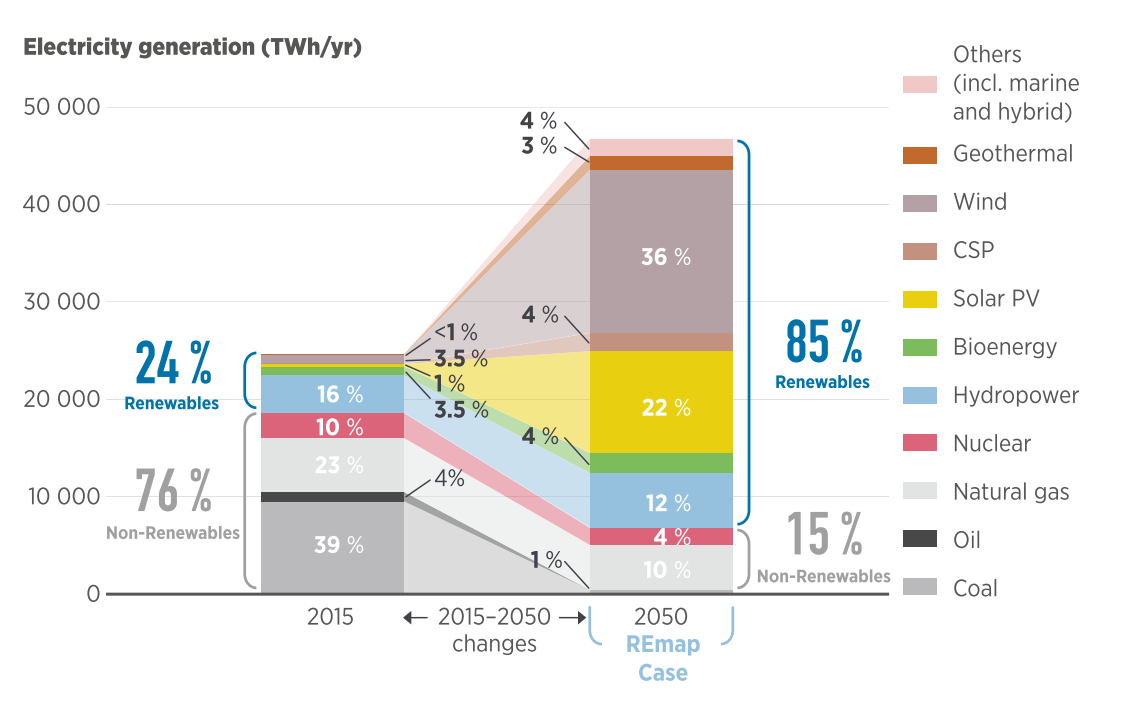
\includegraphics[width=1\columnwidth ]{ChapterIntro/Figures/irena_scenarios.png}
	   %\vspace*{-8cm}
		\caption{Renewable Energy Sources penetration scenario. Extracted from \cite{IRENA2018}}  
		\label{fig:scenarios}
\end{figure}


\section{Smart Grids. The evolution of the electrical network}

%\subsection{Electricity network}
The physical infrastructure of the electricity network is composed by generators, transmission network, distribution network and end-users or consumers, as shown in Figure \ref{fig:ree}. 

\begin{figure}[h]
	\centering 
	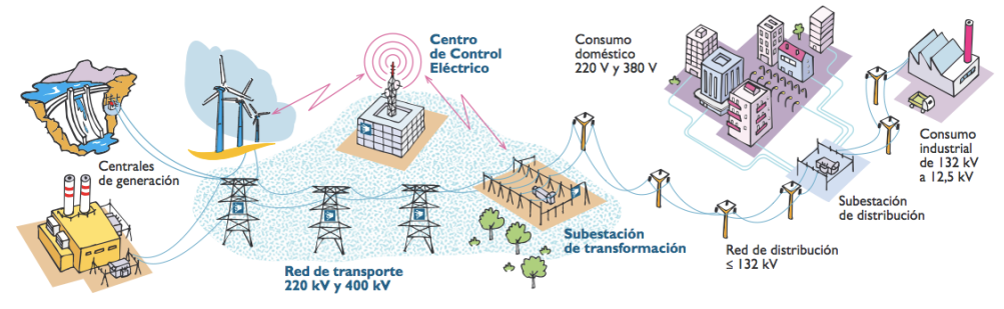
\includegraphics[width=1\columnwidth ]{ChapterIntro/Figures/ree.png}
	   %\vspace*{-8cm}
		\caption{Electricity network scheme. Extracted from \cite{RedElectricadeEspana}}  
		\label{fig:ree}
\end{figure}

Generators are the main agents feeding the grid downstream. Large generators can produce a range from 6 kV to 20 kV \cite{Gomez-Exposito2008}, to then increase the voltage up to 200 kV in order to connect to the high voltage (HV) tramission lines. The transmission network is the responsible for the electricity transportation over long distances, and it is done at HV level. By doing this, the transmission losses are lower while using a cheaper infrastructure. The tranmission network voltage level usually ranges from 200 kV to 1000 kV \cite{Erbach2016}, and both generators and HV-MV transformers are the main elements connected to it. Due to their critical position in the system, connecting generation and consumption sides, transmission grids are meshed to avoid collapsing when there is any failure in on of the lines. On top of that, this layout allows the distribution of the loads through different tramission lines with the objective of reducing losses and avoiding congestions. Transmission networks are operated by the so-called Transmission System Operators (TSO). Similarly, distribution networks are responsible for the energy distribution and transportation for shorter distances. One could consider a distribution grid when its voltage levels are either medium-voltage (MV) and low-voltage (LV). By definition, the voltage levels considered for distribution networks are: 132 kV, 66 kV, 45 kV, 30 kV, 20 kV, 10 kV, 6 kV, 3 kV, 1 kV, 400 V and 230 V \cite{Gomez-Exposito2008, Erbach2016}. 

Differently as seen in the transmission system, the assets connected at distribution level are mainly loads ranging from industrial loads, connected at MV, to residential loads, most usually connected at the LV level. However, generation units can also be connected  at the distribution level, usually only considering renewable sources. The configuration layout of distribution networks is commonly not redundant, meaning that they do not usually use meshed configurations. As a result, these networks are not as redundant as the transmission system. Hence, this could lead to problems when DERs are connected to MV or LV connection points, leading to congestions  in distribution networks that were not expected when the network was implemented. Distribution networks are managed by Distribution System Operators (DSO), who connect consumers, install electricity meters and communicate the end-user consumption to energy suppliers or retailers \cite{Erbach2016}. An overview of the previously mentioned elements is shown in Figure \ref{fig:networkscheme}. 


\begin{figure}[h]
	\centering 
	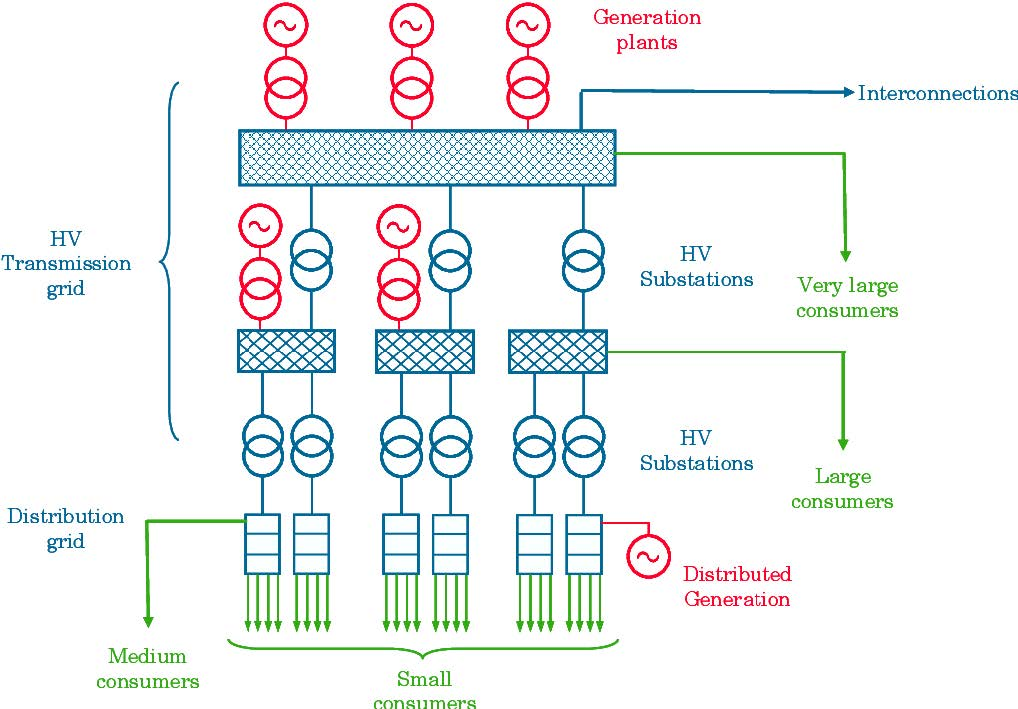
\includegraphics[width=0.8\columnwidth ]{ChapterIntro/Figures/ELECTRICITY_SYSTEM.jpg}
	   %\vspace*{-8cm}
		\caption{Electricity network scheme. Extracted from \cite{Erbach2016}}  
		\label{fig:networkscheme}
\end{figure}

%\subsection{Smart Grids}

Despite the scenarios where renewables are the main source for electricity production, it is a fact that geographical, economical and social-cultural barriers are still slowing down the implementation of renewable energy projects in some locations in the landfield \cite{ASANTE2020111479, barriers2020}, leading to newer technologies to allocate renewable sources in places where a larger power output can be obtained, and generally less concern by end-users in terms of environmental and visual impact of them, such as off-shore wind turbines \cite{Kaldellis2016, KPMG2019}, connected to the transmission network. At the same time, as electricity demand on grids increased due to the electrification of appliances, distribution system operators (DSOs) started to face congestions in their networks, and hence utilities started to find solutions for managing these peak loads, usually located in specific time periods.  This combined to the implementation of smart meters so utilities could encourage customers to switch consumption from peak to non-peak hours, and the need for monitoring and controlling the operation of the distribution network enhanced the development of smart grids. Traditionally, electric power systems have been centralizsed structures organized into generation, transmission and distribution, placing end-users and the endpoint of the supply chain. This was an unidirectional structure where electricity generated by large power plants was transported by means of transmission and distribution networks, to be delivered to end-users. 

Furthermore, the emergence of the social awareness of the environmental impact of the end-users consumption, the increase of the electricity prices, as well as the emergence of the so-called distributed energy resources (DERs), such as small-scale PV installations (mainly rooftop), storage systems, electric vehicles (EVs) and smart home appliances are transforming the end-users into active participants in the power system. The increasing penetration of these decentralized resources, as well as the emergence of new market agents like prosumers, aggregators and active consumers, are pushing the electricity system to include innovation in their business models, creating the paradigm of smart grids (Figure \ref{fig:IRENA-DSO}). According to \cite{EuropeanParliamentSG}, smart grids can be defined as:

\begin{figure}[h]
	\centering 
	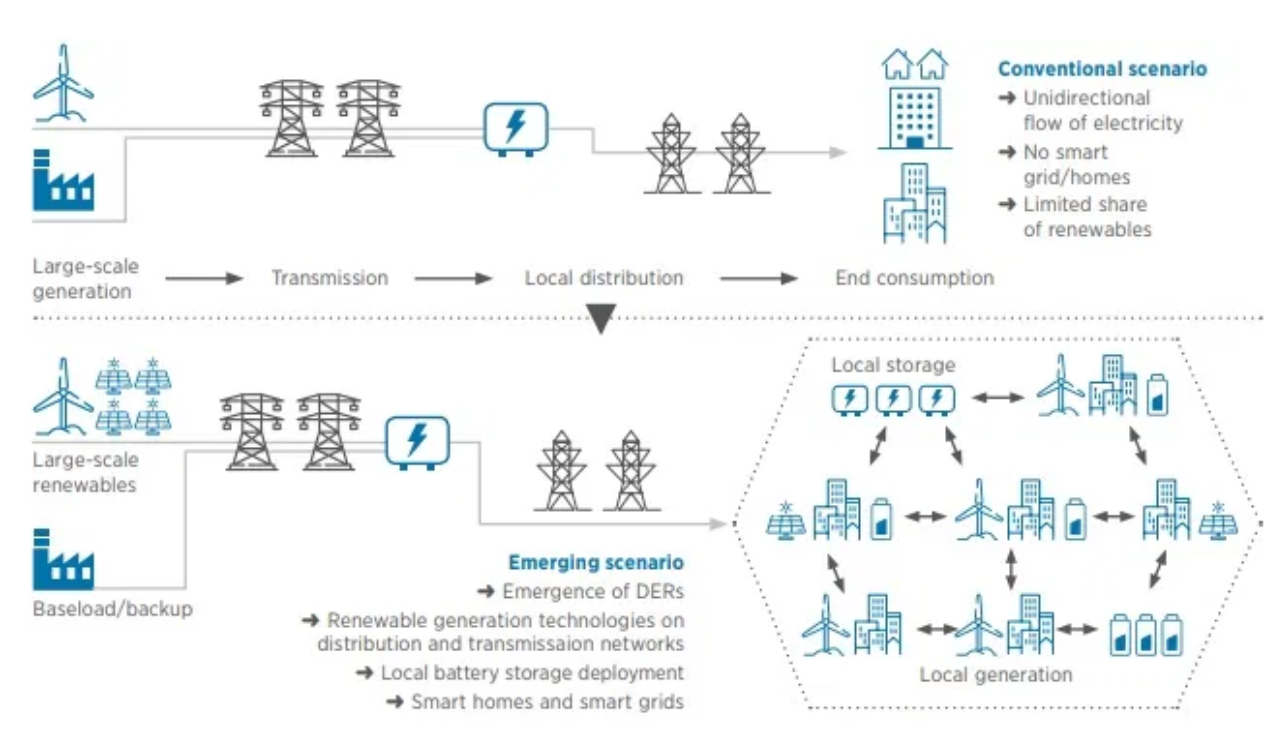
\includegraphics[width=0.9\columnwidth ]{ChapterIntro/Figures/Irena-DSO-1.png}
	   %\vspace*{-8cm}
		\caption{Conventional scenario vs Smart Grids. Extracted from \cite{IRENA2018}}  
		\label{fig:IRENA-DSO}
\end{figure}




\begin{tcolorbox}
\textit{"an electricity network that can integrate in a cost efficient manner the behaviour and actions of all users connected to it, including generators, consumers and those that both generate and consume, in order to ensure an economically efficient and sustainable power system with low losses and high levels of quality, security of supply and safety".} 
\end{tcolorbox}

However, it is not only in terms of technological innovation to fulfill the electricity transition roadmap. Changing the regulatory framework mainly for DSOs to adapt the current regulation for the operation of the distribution network to the new challenges placed by DERs is a key factor for the success of the energy transition.

With the liberalisation of the electricity markets all over Europe, due to the promotion of directives such as the ones in the First, Second and Third Energy packages \cite{EuropeanCommission2003, EuropeanCommission2009} to create a more robust internal market \cite{Hancher2017, EUPHEMIA2016, antonopoulos2020nodal}, grid planning faced problems related to generation forecast. Because at that point the generation at the HV side of the grid was not 100$\%$ planned anymore. However, the network overcame the problem establishing rules where these new agents must inform of their operations a centralised organisation in order to maintain the balance of the system, and creating a markets-system where TSOs upload their needs and generators their offers. 

Nowadays the EU is promoting another change in the structure of the electricity market, imposed by the need to decarbonise the energy sector by 2050 and the willingness to empower the citizen changing its role from pure consumer to a new agent in the market \cite{Hancher2017}. This is mainly going to be done by promoting the integration of DERs in the distribution grid which supposes an entirely new approach to the grid management. Challenges like reverse power flows and an increase of voltages near the point of coupling, among others, will arise. This structural change of the electricity system has been changing habits in the sector for some years now, and with these new ways to proceed challenges have arisen, from \cite{Bollen2011} the main changes can be classified as:

\begin{enumerate}
\item With the liberalization of the generation, system operators are less capable of limiting
connections of new generation assets which can drive the grid, at some locations, to its
limits.
\item Formerly traditional PGMs location was determined considering the interests of the system
operator and the constraints related to the construction of such large power plants.
Nowadays, the location of new RES power plants is instead related to energy source availability.
\item RES generation tends to connect at distribution level instead of transmission level where
all the main PGMs were connected.
\item Democratization of generation assets which, other than the new cases stated above, can
transform traditional passive-customers to active customers and thus increase the variability
of the demand.

\end{enumerate}

These four changes in the power system structure can and will be an improvement in terms of clean generation, increased energy efficiency, customer empowerment, and grid reliability, among others. However, the truth is that nowadays most of the European grids are far from being ready to face such challenging opportunities and these new approaches are also making arise new problematic, and not-so-new ones, that can be divided into two main groups: 
\begin{enumerate}
\item Generation and load balancing: If there is no balance between generation and demand, the frequency of the system starts to deviate from the nominal value; this may be a problem for some electric/electronic loads. However, the main concern arises when large generators are synchronous machines. In an intense frequency deviation event some generators may trip from the grid, causing even a harder frequency deviation. This domino-like problematic is called cascade tripping and can lead to a local or even "global" system blackout. This problematic has been a concern for the system since its beginnings because the load forecast is not always accurate. However, large PGMs can be mandatorily disconnected from the grid for safety purposes \cite{Bollen2011}. Then, the challenge increased with the liberalization of the generation market. Nowadays, with the introduction of DERs and the empowerment of the user via demand-modulation strategies, the future forecast of generation and demand is expected to be more challenging than ever.

\item Distribution grid congestion: Grid congestion, mainly at TSO level but also at DSO level,has always existed. However, due to the traditional operation of the grid, the fit-and forget approach consisting of investing in expanding the infrastructure was the most costefficient approach at the distribution level. With the uncontrolled connection, in terms of number but also location and characteristics, of new DER assets to medium and low voltage grids, a new grid structure may be needed from the fit-and-forget perspective. However, this does not seem either rational nor cost-effective viable, and instead, these new congestion challenges will need to be addressed from an active (real-time) management approach.
\end{enumerate}


\section{Regulation framework and new agents in the energy transition}
For the last 15 years global warming awareness and a more rational approach to production and consumption of goods and habits have been an increasing concern for societies with a firmly established welfare state. Related to this new approach, electricity markets have been the target of criticism due to their massive contribution to the emission of greenhouse effect gases \cite{Hancher2017}. Within the European energy policy context, the chosen way to carry out this reduction of emissions by the energy sector is enhancing a higher penetration of DERs (particularly RESs) in distribution networks. This positioning, while has multiple potential benefits for the grid and its agents, also sets out new challenges to be faced.
All the perks and disadvantages of a higher share of DERs need to be adequately regulated in order to keep secure the functioning and operation of the grid. It also has to be noted that inside the EU energy policies, the environmental concern is nowadaysone of the main drivers. However, there are also other key objectives to achieve, which in some cases will present synergies, but in other cases, could collide among them. 

The creation of the Winter Package the year 2016, also known as Clean Energy Package for all Europeans \cite{validzic2017clean}, started after the European Commission had evaluated the performance of the Third Energy Package established in 2009.  After assessing the outcomes of the previous energy packages, the objectives starting back then could be grouped in three, as follows: 
\begin{enumerate}
\item Adapting to the decentralization of the power system. 
\item Empowering customers and citizens. 
\item Ensuring the internal market level playing field. 
\end{enumerate}

About the CEP itself, first it has to be knownthat it is a set of regulations and directives published in June 2019 to promote the energy transition started with the Third Energy Package back in 2009. Among the CEP regulations and directives, the ones that address the electric sector are the e-Directive (EC 2019/944; \cite{Directive2019944}) and the e-Regulation (EC 2019/943; \cite{Directive2019943}), whose subject matter and scope is centred in \textit{"setting the basis for an efficient achievement of the objectives of the Energy Union and in particular the climate and energy framework for 2030"} (e-Regulation), \textit{"via the creation of common rules for all the assets connected to the power system, with a view to creating truly integrated, competitive, consumer-centred, flexible, fair and transparent electricity markets in the Union"} (e-Directive). The e-Directive and e-Regulation are mainly focused towards the creation of market models to
promote the energy transition. In terms of market design there is a group of markets, local energy and flexibility markets, that can be crucial to promote the widespread of new agents and technologies \cite{Xu2019}.


\section{Flexibility as a service for the energy transition}
Power system flexibility will play a key role in the energy transition and the next generation electric grid, and some of the main outcomes of implementing flexibility are the possibility to replace fossil fuel generators with clean and renewable energy sources; increase reliability and resilience against disruptive events; improve performance and reduce cost of new and existing assets and achieve the scenario where a low carbon economy is possible. 

In general terms, flexibility can be defined as follows, according to the International Smart Grid Action Network (ISGAN)\cite{Hillberg2019}.

\begin{tcolorbox}
\textit{"The ability of a power system to reliably and cost-effectively manage the variability and uncertainty of demand and supply accross all relevant timescales."}
\end{tcolorbox} 

Traditionally, these variations from the demand side have been overcome by means of fuel-based flexible large generators such as carbon and gas turbine; and pumped hydro power plants, which were forces to be able to provide flexibility. Those changes in the demand-side where mainly from changes in the load consumption based on consumer behavior.
Some of these requirements for large generators are still considered in the new regulation under the Clean Energy Package and Grid Codes \cite{validzic2017clean}. However, most of the requisites are not mandatory for smaller generator units, and with the new paradigm where there is a reduction in the number of synchronous generators and more difficulties to forecast demand and generation, the remanining generator units might not be able to handle the flexibility required to keep the grid consumption and generation balance. This will suppose an increased need for flexibility \cite{Xu2019}. Besides, the increasing penetration of DERs into the MV and LV grid will suppose some challenges in terms of network operation, which will need to be addressed by the DSOs by means of active management and flexibility activation to avoid grid reinforcement. For these reasons, flexibility markets are being recognized in the e-Directive \cite{Directive2019944} as a key element to support a safer and more efficient use of the already existing grids.
According to the same institution, flexibility will enable all stakeholder and elements of the grid considering generators, consumers/end-users, storage and infrastructure to be active participants in the energy system, also enabling the cost-efficient development of RES and more resilient power systems \cite{Hillberg2019}.  

\begin{figure}[h]
	\centering 
	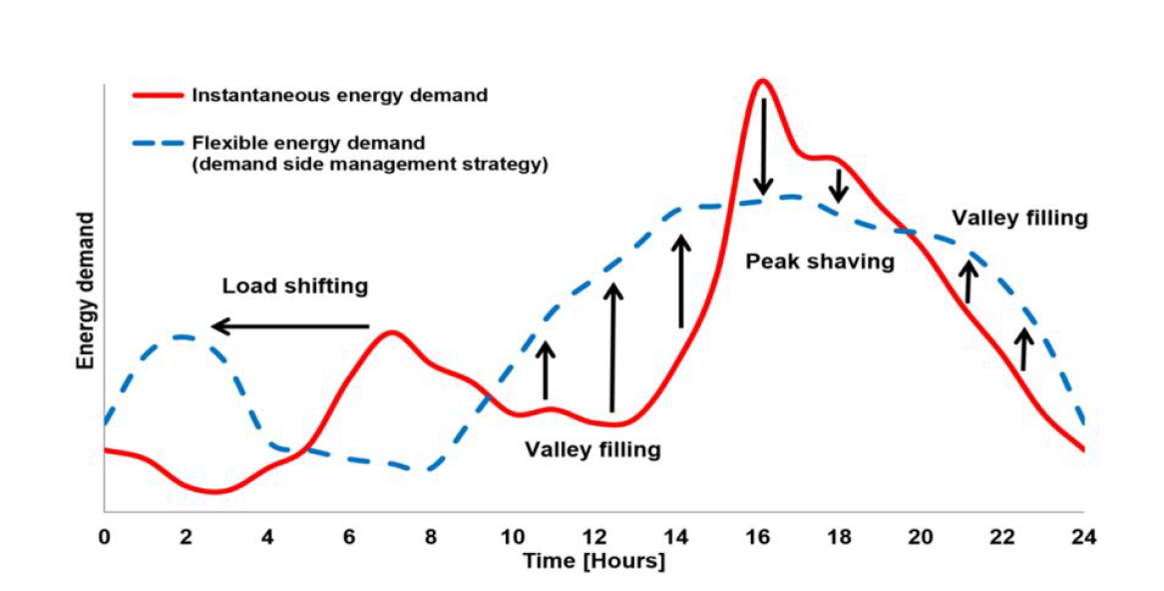
\includegraphics[width=1\columnwidth ]{ChapterIntro/Figures/flex_load_shifting.png}
	   %\vspace*{-8cm}
		\caption{Flexibility effects on electricity consumption. Extracted from \cite{Hillberg2019}}  
		\label{fig:load_shifting}
\end{figure}


Due to the increase of electricity consumption and DERs integration in the last 10 years, the consumer behavior patterns have been broadly studied \cite{ZHOU201773,TORRITI2014265}, showing that the electricity consumption is focused at specific time periods, such as noon and in the evening. With the implementation of DERs and the increase of the electricity consumption, there is a possibility to include flexibility in power systems by achieving the paradigm where consumption follows the generation curve only partially. That could lead to implement flexibility in the demand-side by shifting the consumption of some assets or the production of some small scale generators or storage systems to other time periods, as seen in Figure \ref{fig:load_shifting}. Demand-side flexibility can be defined as follows, accordint to \cite{EuropeanSmartGridsTaskForceExpertGroup32019}.  

\begin{tcolorbox}
\textit{"The ability of a customer or prosumer to deviate from its normal electricity consumption or production profile, in response wo price signals or market incentives"} 
\end{tcolorbox}

Demand-side flexibility is based on load, demand-side generation and demand-side storage. The Universal Smart Energy Framework (USEF) defined a wide range of services that could be provided to network operators, retailers, balancing parties thanks to demand-side flexibility under demand-side management. An overview of the flexibility products can be seen in Figure \ref{fig:DSF}. 

\begin{figure}[h]
	\centering 
	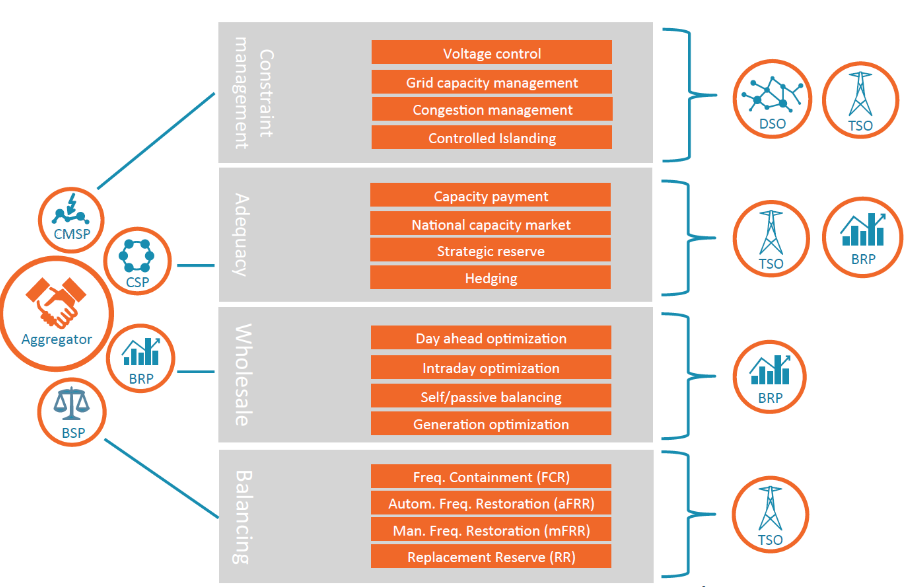
\includegraphics[width=1\columnwidth ]{ChapterIntro/Figures/USEF_DSF.png}
	   %\vspace*{-8cm}
		\caption{Products and services available from the demand-side. Extracted from \cite{USEFFoundation2015a}}  
		\label{fig:DSF}
\end{figure}


\section{Sustainability of smart grids and DERs}
Sustainability can be understood as a progress model that considers not only economic, but also environmental and society needs in order to develop an economic model that maintains an ecological balance. The 2030 Agenda for Sustainable Development, agreed by all United Nations Member States, defined 17 goals calling for action by all countries with the objective to achieve a sustainable and prosper future \cite{SDGOALS2015}. Many of the goals are aligned with the energy transition roadmap, and with the implementation of demand-side activities for encouraging end-users as market participants. Objectives 7, 11, 12 and 13 of the Sustainable Development Goals for 2030 (Figure \ref{fig:sdg}) are related to the previous statement, encouraging all Member States to include sustainability when planning the electricity system and market of the near-future.  

\begin{figure}[h]
	\centering 
	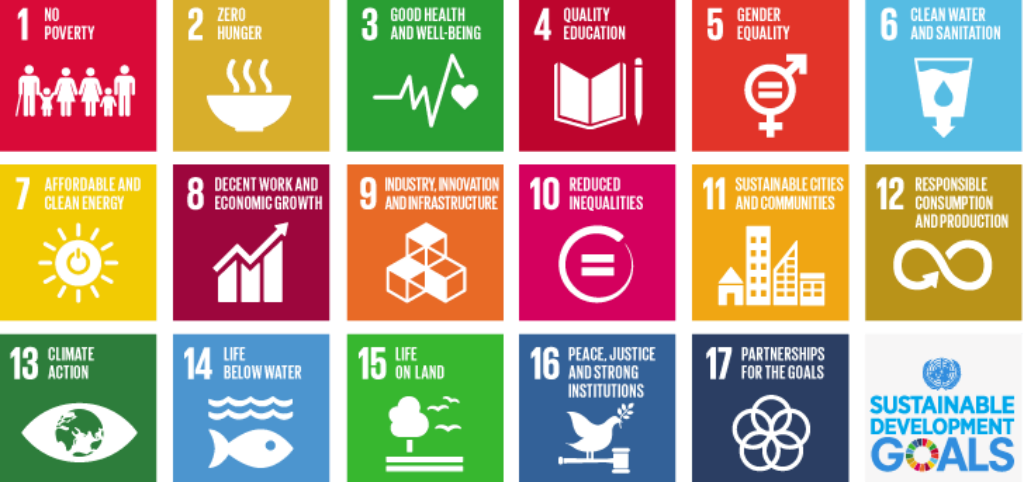
\includegraphics[width=1\columnwidth ]{ChapterIntro/Figures/SDG.png}
	   %\vspace*{-8cm}
		\caption{Sustainable Development Goals defined by the United Nations.}  
		\label{fig:sdg}
\end{figure}    

The increase of renewable generation has provided and is providing many benefits in the road towards a decarbonized power system. However, in the past years, social concerns about the environmental impact of renewable technologies have arisen \cite{Temper2020}, with more than 3000 environmental conflicts based on renewable energy-related projects. These problems are based on the fact that these projects do not take into consideration neither the acceptance of the population living close to the renewable energy plant location, nor the consequences of having the power plant, such as the reduction of agriculture fields or the impact on the land prices. 


The decentralization of the renewable generation with the appearance of DERs has a large potential to succeed in the energy transition roadmap. However, sustainability must be taken into consideration in each and every step, even in local energy communities and DERs \cite{AMPONSAH2014461}.
% It can be seen as the intersection of the previously mentioned three concepts, as outlined in Figure \ref{fig:sust}.

Some of the current methodologies for calculating the environmental impact of renewable energy technologies assume that the carbon footprint of renewable sources is zero, because they only consider the $CO_2$ emission factor under the operation phase \cite{IRENA2020}. Renewable energy technologies, Electric vehicles and storage systems can be carbon neutral under the operation phase, but they are not zero, and their contribute negatively to other environmental indicators when considering the entire life cycle. There is a non-negligible carbon footprint or other environmental impacts such as water usage and polution and ozone contribution that must be considered \cite{en12214214, Moro2017, Jiang2018}. Furthermore, when developing smart grids and renewable energy sources and energy transition policies, a previous analysis should be performed in order to understand the current installed capacity in the country, in order to lower the environmental impact by implementing such technologies \cite{Treyer2014}.
%
%\begin{figure}[h]
%	\centering 
%	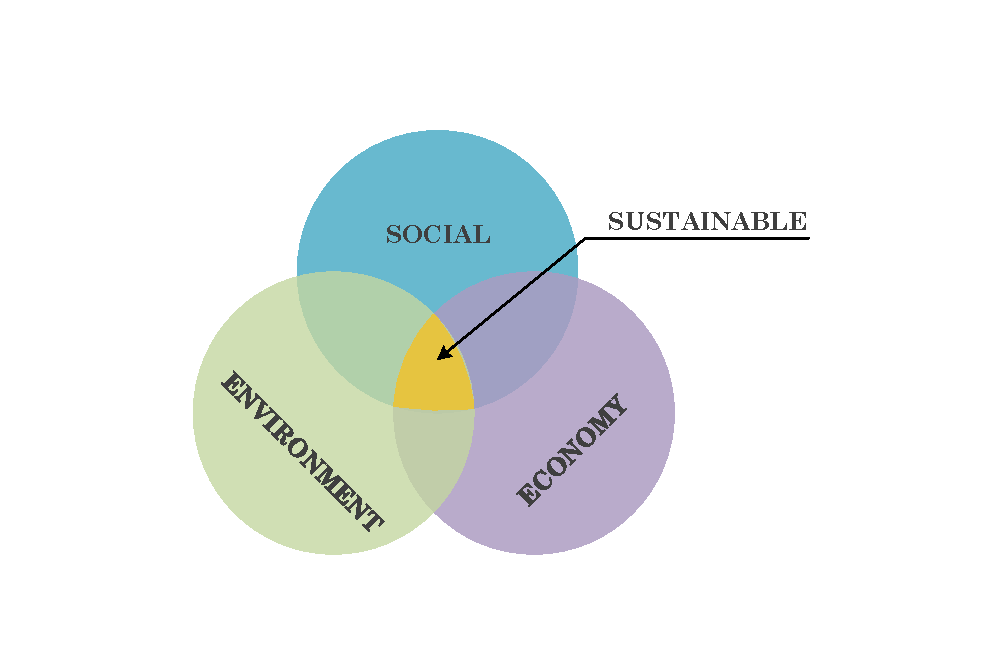
\includegraphics[width=0.7\columnwidth ]{ChapterIntro/Figures/SUSTAINABILITY.pdf}
%	   %\vspace*{-8cm}
%		\caption{Definition of sustainability.}  
%		\label{fig:sust}
%\end{figure}

Technologies and methodologies such as circular economy, second-life options for storage systems, and life-cycle assessment (LCA) are key to check the viability of renewable energy projects and smart grids implementation. More specifically, LCA is a powerful a tool for assessing environmental impacts of renewable energy sources, so as to assess the environmental impact based on indicators of renewable energy technologies and smart grids throughout the entire lifecyle. 



\newpage 
\section{Objectives and scope}
Several past and recent works in the literature have dealt with the development of smart grids and defining local electricity markets for enhancing the energy transition. The majority of these studies are based on DERs integration, optimization at household level and forecast of indivual assets. The majority of these studies consider flexibility as a known signal, assuming a perfect forecast and a direct control of the flexible assets, as a way of simplifying the operation of the local flexibility markets. Furthermore, they assume that both the aggregator and the DSO share information regarding the flexible assets or the network layout, or can even control the flexible assets or the network. The fact is that, in reality, and according to the current regulation, they must be different entities, and as a result they might differ in the business model. Furthemore, even though there is a significant amount of data being collected at different points of the power system thanks to smart meters rolling out and more information and communication technologies (ICT) installed, there is still a difficulty to get access to this data. As a result, the access to data is still a challenge for smart grids agents to develop innovative algorithms and solution for the energy transition era. Combining the previous facts and challenges, the main research question that this thesis aims to answer is the following one:

\begin{tcolorbox}
What are the possibilities to develop and activate flexibility in distribution networks, by engaging demand-side and ensuring that the sustainability goals are taken into consideration, considering data-driven approaches and challenges? 
\end{tcolorbox}

This can be considered a broad question, and hence the knowledge barriers should be found in order to establish the baseline for the PhD research. This manuscript aims to answer this question focusing on the role of the demand side and their flexible assets and what the benefits and consequences would be for distribution networks, managed by DSOs. Figure \ref{fig:objectives} provides an overview of the system under study, considering the demand-side by means of prosumers and flexible assets; the aggregator as the entity that collects all the available flexibility and provides this service to the DSO by controlling the end-user's assets; the DSO as the main client of this flexibility; the electricity market to understand which role plays the flexibility in a market-environment; and lastly the environment, to assess the global warming potential and other environmental impacts that flexibility could reduce or increase. Based on the previous discussion, more specific objectives can be outlined in order to set the basis for the research developed in this thesis. The research questions that led to the objectives of the thesis are outlined below: 

\begin{tcolorbox}
\begin{enumerate}
\item What are the possible market schemes to integrate DERs and demand-side management, while at the same time ensuring that network operators can benefit from these services?  
\item How can flexibility be defined and modeled, based on the final users providing and using this flexibility, as well as the time horizon purposes? 
\item How can flexibility be forecast, from the aggregator point of view, with very limited amount of data available, in a fast and reliable approach so as to know in advance the flexibility available in the portfolio, in order to provide flexibility to DSOs for operation purposes?
\item How can this flexibility help DSOs to mitigate or avoid congestions in MV networks, and how can this flexibility request be calculated so as to be economically better than investing in network expansion or hosting capacity?
\item How this scenario of flexibility provision can be environmentally assessed, so as to know if these approaches can be included in each and every country? Should the current installed capacity and generation portfolio be taken into account before the deployment of flexibility services in smart grids?
\end{enumerate}
\end{tcolorbox}

A conceptual overview of the different objectives outlined above is shown in Figure \ref{fig:objectives}, which can be also understood and the steps taken in this thesis. Each of the questions and objectives can be detailed and related to each of the chapters of this manuscript, as follows: 

\begin{enumerate}
\item \textbf{Analysis of the market schemes for energy and flexibility for the development of smart grids.} The first step of the thesis has the objective of defining the framework where new products and services can be implemented, with the purpose of providing smart grids stakeholders such as retailers, network operators and end-users a set of benefits. Special focus is set in energy and flexibility services for balancing agents and distribution network operators, with the creation of new market agents like the aggregator and the local market operators. Different market mechanisms for providing these services are analyzed, considering peer-to-peer and peer-to-platform approaches. 
\item \textbf{Definition of flexibility based on the main stakeholder, time horizon and business objective.} As a result of the previous state-of-the-art analysis, the research is focused on flexibility for the distribution network operator. The main research gap to address here is that distribution network operators require flexibility for the network operation, however current research still lacks a common definition for flexibility, and how can this flexibility be formulated based on the final user and the final approach of this flexibility. There are several differences to be considered if this flexibility is implemented for operation purposes or planning purposes. In this case, the role of the aggregator, the information exchange between these two agents as well as the regulation behind them are key for the development of successful flexibility services for the DSO.  
\item \textbf{Modeling and forecasting flexibility of an aggregator's portfolio based on statistical techniques.} Based on the result of the previous objective, a modeling and forecasting approach is developed under this objective of the PhD research. This methodology is based on a bottom up approach for collecting the flexible assets' submetering data, and later a hierarchical approach is performed with the approach to estimate the available flexibility in a two-level hierarchy. The underlying forecasting technique is based on statistical learning, considering several approaches. The benchmark model is defined by means of a particular case of the moving average, known as climatology model; and also considers the simple exponential smoothing. The more complex methodologies for forecasting the flexibility value is based on a conditional approach, and implementing probabilistic forecast by means of kernel density estimation and recursive maximum likelihood. This methodology is later implemented to a case study of an aggregator's portfolio to assess the goodness of fit. 
\item \textbf{Development of an optimization algorithm for the distribution network operation under congestion management scenarios.} Once the flexibility has been forecast by the aggregator, this service can be provided to the DSO for the correct operation of the distribution network. The research performed under this objective aims to provide DSOs with a tool to calculate the flexibility required for avoiding a congestion in the distribution network. This is implemented by means of an AC-OPF algorithm, with the main objective function of minimizing the flexibility activation costs that the aggregator should pay for it. The final purpose of activating flexibility in distribution networks is for DSOs to avoid the reinforcement of the network and activate flexibility instead. 
\item \textbf{Analysis of the environmental impact of the current electricity market generation scheme and evaluation of environmental savings by implementing flexibility.} The final step of the research aims to assess the whole idea and approach by evaluating potential savings in terms of $CO_2$ emissions in the generation profiles, based on a cradle-to-gate life cycle assessment methododology. This study defines a peak hourly LCA approach to highlight those time periods where flexibility could be activated and evaluate the environmental impact of these time periods. This methodology is implemented in five case studies in Europe to assess whether there are environmental savings or not. This approach can help policy makers to implement smart grids and energy transition initiatives not focusing only on the technical development, but also in terms of sustainability. 
\end{enumerate} 

\begin{figure}[h]
	\centering 
	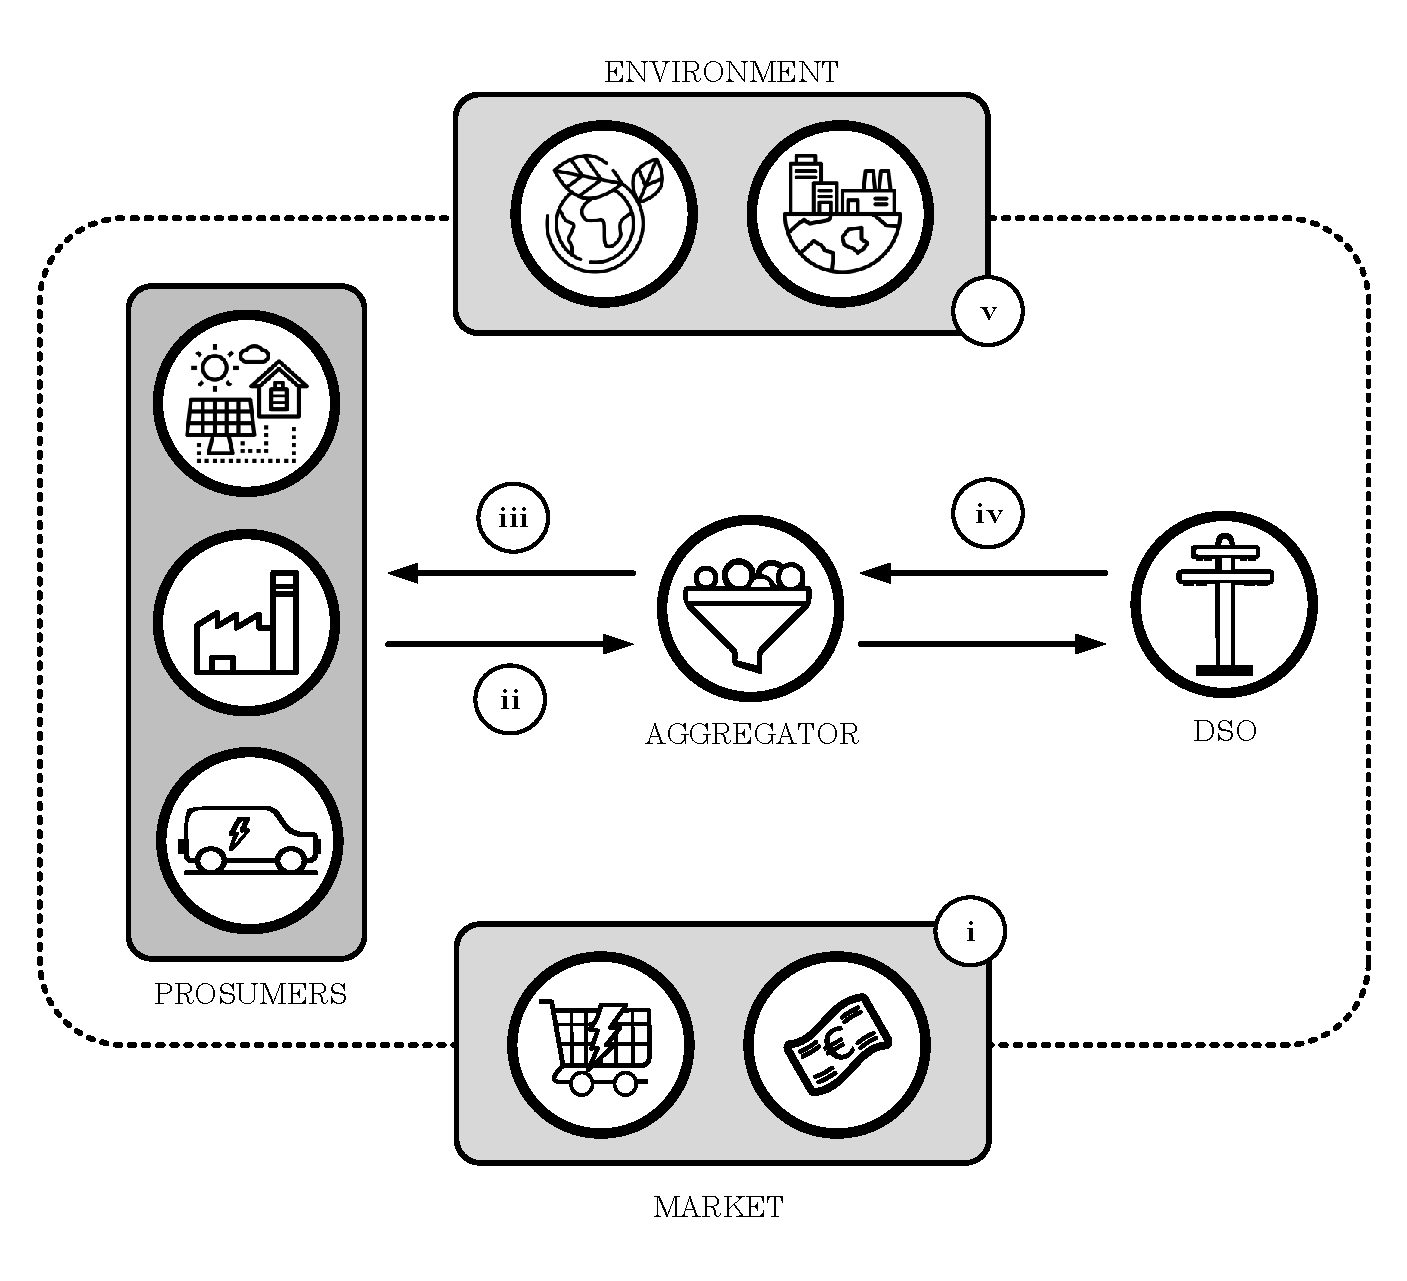
\includegraphics[width=0.75\columnwidth ]{ChapterIntro/Figures/objectives_figure_2.pdf}
	   %\vspace*{-8cm}
		\caption{Overview of the thesis objectives}  
		\label{fig:objectives}
\end{figure}



\newpage 
\section{Thesis related work and activities}
This section provides a summary of the work and the relevant activities that the author has participated in during the developlment of the thesis presented in this manuscpript. 
 	
Doctoral activities started in June 2017 with the collaboration on behalf of the EMPOWER \textit{Local electricity retail markets for prosumer smart grid power services } Project (Grant Agreement No. 646476). This work consisted on a review of the current state of the art in terms of Life Cycle Assessment Methodology in the field of smart grids, the understanding of how this methodology can be implemented in power systems and renewable energy technologies and the assessment of the environmental impact of the pilot-sites implemented throughout the project. This research resulted in a presentation in the General Assembly of the H2020 Project [P-C1] and the technical report [TR-2]. The research on the environmental assessment of ICT and Smart grids continued in the H2020 Project INVADE \textit{Integrated electric vehicles and batteries to empower distributed and centralised storage in distribution grids} (Grant Agreement No. 731148), in years  2018 and 2019, with the assessment of the environmental impact of electricity generation and the possibility of including flexibility to lower the environmental impact of electricity production in the INVADE pilot-sites. This research was performed in collaboration with the Finnish research center VTT, NTNU, Elaad and eSmart resulted in the journal publication [J1], a conference proceeding [C2], and technical reports [TR3], [TR5]. Dissemination events for the exploitation of the results took place in years 2019 and 2020, [P-C5] and [P-C11]. 

Since the main objective of the thesis is how new local markets and new service can help the deployment of smart grids, a thorough review of the state-of-the-art on local electricity market was done as a starting point of the doctoral research in 2018. This research was mainly focused on describing the basics on power systems and market mechanisms, as well as a literature review on local and micro-markets. As a result of that, a technical report was developed [TR1], and two book chapters were published by Wiley ([BC1],[BC2]).  The evolution of this state-of-the-art review, combined with the collaboration with colleagues at CITCEA-UPC and other research centers and companies such as EYPESA and Smart Innovation Norway or on behalf the INVADE Project led to several outcomes covering from technical reports [TR4], journal articles [J4] adnd [J5]; conference papers [C1], [C3] and [C4]; and presentations in local and international events [P-C3] and [P-C4].  

The evolution and implementation of smart grids based on data-driven approaches has been of interest of the author, and combined with collaboration with other universities as KU Leuven, DTU and KTH Stockholm on behalf of EIT InnoEnergy, resulted in [P-C6], [P-C10] and [P-C14]. 

%Escriure BD4OPEM aquí 
Year 2020 started with the kick-off the BD4OPEM H2020 Project \textit{Big Data for Open Innovation Energy Marketplace} (Grant Agreement No. 872525), with the participation of 12 partners from 8 different countries, and 5 pilot-sites. The research consisted on the development of algorithms for flexibility forecast and distribution network congestion management based on optimization techniques and flexibility provision. This work was combined with the Technical University of Denmark (DTU) under the external stay of the author, and in collaboration with other research centers and companies such as JSI and ICOM. This work resulted in a technical report [TR6], two dissemination events [PC-12], [PC-15], and three journal publications under review or preparation [J2], [J3] and [J6].  

The international placement took place from March 2020 until April 2021, at the Electricity Markets (ELMA), DTU, Kongens Lyngby, Denmark. The topic was aggregated flexibility forecast based on probabilistic forecast techniques. It resulted in a journal paper [J2], and the database publication [DB1]. During this period, the author has collaborated with KU Leuven in the core of the Data Science Working Group, with the aim of improving the knowledge of undergraduate students in the field of data science in the energy sector. This resulted in the publications [J7] and [J8]. 

Since the author and the research center where the thesis was involved has a flair for knowledge transfer and higher and professional education, the author has collaborated with other entities and other researchers, resulting in the respective outcomes, which are not included in the thesis manuscript. This is the case of the collaboration with EIT InnoEnergy. This European institution has as a main core activity the connection and collaboration between industry, universities and research centers with the objective of reducing the gap betwen research and the market. In years 2018, 2019 and 2020 the author has been the lead teacher of the course on Control and Automation for the Efficient Use of Energy, developing the open-source learning material and developing a course based on project-based learning and flipped classroom approach. This resulted in several activities, such as [E1] being the learning material, and dissemination of the results in different local conferences [P-C2], [P-C7] and [P-C8]. The project Learning Analytics started in September 2018, with the objective of monitoring students' performance to assess their engagement in the course, in collaboration with the Data Collection company DataLemon. This collaboration led to dissemination event [P-C9] and [P-C13], as well as an ongoing journal paper to be submitted in the near future. Other collaborations within the Electrical Engineering Department led to two outcomes: a MOOC courses for wearable technology [E2], and a publication in a local journal [C5]. 


%\newpage 
\section{Thesis outline}
The content of the thesis is organized in the following chapters as follows:
\begin{itemize}
\item \textbf{Chapter 2} presents the overall state-of-the-art in terms of local energy markets, in order to define the role of flexibility in a local market and to which extent this service can help energy transition, and more specifically, DSOs. This work correspond to the first objective of the thesis \textit{(i)}. 
\item \textbf{Chapter 3} outlines how flexibility can be formulated, defined and modelled according to different approaches in terms of end-user, approach and time-horizon, covering the second objective of the thesis, providing different formulations for modeling flexibility \textit{(ii)}. 
\item \textbf{Chapter 4} presents the aggregated flexibility forecast for estimating the available flexibility within an aggregator's portfolio, with limited amount of information, for operation purposes and trading in a market or a bilateral contract. This chapter aims to fulfill the thirds approach of the thesis \textit{(iii)}. This formulation is implemented under a case study covering a portfolio of flexible assets such as Electric Vehicles, Space heaters and electric water boilers.  
\item \textbf{Chapter 5} outlines the AC-OPF formulation for calculating the flexibility requests needed by DSOs to solve congestions in MV networks by means of flexibility activation. This chapter corresponds to the fourth objective of the thesis research \textit{(iv)}.  
\item \textbf{Chapter 6} extends the scope of the previous research assessing the potential role of flexibility in different countries, in terms of sustainability. This chapter calculates the peak-hour environmental impact measured in $CO_2$ emissions, so as to establish a baseline for countries to understand where DERs and flexibility could be implemented and leading to a lower carbon footprint. This chapter focuses on the last objective of the research \textit{(v)}. 
\item \textbf{Appendix A} enumerates the publication and research outcomes both related and non-related to the thesis manuscript. 
\end{itemize}



\renewcommand\labelenumi{(\roman{enumi})}
\renewcommand\theenumi\labelenumi

\chapter{Providing Flexibility in a local markets}
\label{chapterMarkets}

\chaptermark{Local Markets}
\section{Introduction}
There are many concepts in the field of power markets that are being formulated at the current time: local electricity markets, local markets, local power markets, smart city marketplaces, micro markets, microgrid energy markets, etc.. There is a need to set up the basis of these concepts, to build up the technology that enhances the transition towards a smart grid based on the distribution of locally generated energy instead of big power plants.
This chapter aims to provide the reader with a standardized theoretical background of local and micro power markets so he or she can understand all the agents involved in the energy transition, and thus further research in this field might be performed. Several references are included to prove that right now this topic is of broad and current interest, with many ongoing projects involved.
To start with, the reader will start by asking himself or herself whether there is a need to develop local and micro power markets.
In this chapter, the concepts of local and micro power markets are reviewed and then defined to establish a common reference for their development. The literature review aims to provide an overview of the current status of local and micro power markets. The differences between local and micro power markets are highlighted, based on the literature reviews regarding market design, services, and approach.

\begin{figure}[]
	\centering
	\includegraphics[width=0.7\columnwidth ]{ChapterMarkets/Figures/intro_figure_i.pdf}
	   %\vspace*{-8cm}
		\caption{Chapter objective based on the PhD scope}
	\label{fig:chapter_obj}  
\end{figure}

\section{Why Local and Micro?} \label{sec:why}
The road to local and micro markets comes after years of a centralized market and a rigid structure of the electric power system. Despite this, at present society is facing a globalization movement, where the objective is to simplify entities and structures, and achieve a more homogeneous behaviour of the markets, developing a model that is more predictable, more standardized, and more transparent \cite{Mallet2014}. Besides the energy transition,there is a challenge for distribution system operators (DSO): to connect more than 90% of customers and ever-growing numbers of DERs in a rapidly changing, ever more decentralized, and digital energy world. One
example of this behaviour is the project EUPHEMIA \cite{EUPHEMIA2016}, where the aim is to develop a single price-coupling algorithm, used to calculate energy allocation and electricity prices across Europe, maximizing the overall welfare and increasing the transparency of the prices and flows computations. So why is there a need to go local and micro in terms of energy markets? What advantages does this approach have? The objective of this chapter is to answer the questions faced in \cite{DesignElectricityMarketRossetoo2017}:

\begin{tcolorbox}
To what extent do these concepts offer something new? Aren't these services already offered by suppliers, who can exchange flexibility and energy with consumers, and help them in home automation? Don't current regulation, market arrangements and commercial
practices already allow all this? How can the proposed solutions be made compatible with the natural monopoly of the grid, and deal with the likely conflicts of interest? In activities that present significant economies of scale, thanks to the power of digital devices, what is the advantage of being local and small scale?
\end{tcolorbox}

One of the advantages of being local and small scale is to fulfil the preferences of consumers, as is stated in \cite{faber2014micro}. For instance, some consumers are willing to pay more for the energy they consume if the energy they receive meets their environmental preferences, such being carbon-free, pollution-free, exclusively renewable and locally generated \cite{lane2013costing}. The fact is that the structure and roles of transmission and distribution systems are changing significantly due to the integration of renewable energy sources (RES), in a distributed way, in both transmission and distribution grids. The integration of these DERs along the distribution grid creates local variations that can affect the optimal operation of transmission and distribution networks.

Despite this, local supply variation can be matched with local demand variation, resulting in a local way to solve the problem \cite{mengelkamp2018designing} and producing a potential business model to increase the hosting capacity of the distribution grid without investing in it. This could be the basic idea of a local or micro power market. At present, the existing electricity markets (e.g. wholesale market, balancing market, futures market, and bilateral trading) do not provide to end users the scenarios needed to share their excess of energy or to purchase the surplus of  energy generated locally by the prosumers near that end-user. Local and micro markets are needed to provide new tools to prosumers to empower them to become pro-active and game-changers in the energy (r)evolution that is currently being faced. 

To combine these characteristics in one local market design, there is an additional requirement besides technological development: consumer engagement. The success of local markets would only happen if there is consumer engagement to deal with the energy transition. Due to the energy transition that the power system has faced in the last few years, society has become a key player in this game. Society is prepared right now to face this challenge. Small consumers, producers, and prosumers are becoming more and more active in the way they consume energy. Kalkbrenner and Roosen \cite{kalkbrenner2016citizens} state that citizen participation can be an important means for energy transition at the local level. In this research, a detailed analysis is done to assess whether or not community identity feeling, social norms, and environmental concern can help the implementation of local markets. Also in \cite{kalkbrenner2016citizens}, the promotion of community identity and contacts at local neighbourhood level can facilitate a community feeling, which is key to integrating these new services into smart grids. A local energy community (LEC) can also be based on prosumers who are willing to collaborate with each other and hence to share their investments \cite{sousa2018peer}. In addition, the main aims of prosumers participating in this type of market approach are (i) to reduce costs in their energy bill, (ii) to develop a more transparent energy trading scenario by being able to choose the type of energy source, and (iii) to invest in local and renewable energy production among the community.

The power system was designed based on a top-down approach, which provides reliability and security of supply. Since the integration of DERs along the electrical grid and its natural intermittent behaviour, along with the increase in demand, there has been a change in the way energy is supplied. There is a need to integrate methods of electricity supply \cite{peng2017electricity}, by facilitating the development of LECs, while also maintaining the reliance of the top-down power system, which needs infrastructure investments. In that sense, microgrids can become the main actor to enable the creation of local and micro power markets. 

\section{The evolution of Power Systems} \label{sec:evolution}

Electrical power systems are evolving due to changes in the way electrical energy is produced, transmitted, and distributed. At generation level, the generating plants, predominantly fuel-based in the past, are being replaced by large-scale renewable power plants, for example wind and solar. Furthermore, electrical power generation is nowadays not only concentrated in large centralized power plants connected at high voltage levels but also performed from DERs connected at medium and low voltage levels \cite{Vittal2012}. At transmission level, the traditional system, which was mainly based on high-voltage alternating current (HVAC) lines and cables, is now being extended through high-voltage direct current (HVDC) links that permit bulk power transmission through long distances and the interconnection of asynchronous systems \cite{van2016hvdc}. At the distribution level, DERs are being installed to promote local generation close to consumption sites, leading to bidirectional power flow \cite{series2009microgrids}. All these transformations show how the electrical power system is being reshaped in its generation, transmission, and distribution domains, leading to challenges in its design, operation, and control \cite{miller2015status, farrokhabadi2018microgrid}. 

Focusing on changes affecting the distribution level, small generating and storage units typically in the range from 3 kW to 50 MW, the so-called DERs, are being installed, enabling not only the promotion of RES and local generation, but also the rise of new players in electrical power exchanges. One such is the prosumer, a consequence of the change in the role and behaviour of the consumer, who not only has the ability to consume power but also to deliver it. Currently, new concepts are required for the expansion of active distribution networks, where one of the most promising solutions is based on microgrids \cite{series2009microgrids}.

There is not a single definition regarding the microgrid concept, and its standardization is still missing. Nevertheless, several authors and organizations agree that a microgrid is an electrical network that integrates loads and DERs, and acts as a single entity from both the grid and the market perspective \cite{hatziargyriou2007microgrids, ton2012us}. This book will adopt the microgrid definition of the US Department of Energy (DOE) and reproduced here. A microgrid is 'a group of interconnected loads and distributed energy resources within clearly defined
electrical boundaries that acts as a single controllable entity concerning the grid. A microgrid can connect and disconnect from the grid to enable it to operate in both grid-connected or island-mode' \cite{ton2012us}.

\section{Local and Micro Power Market Concepts} \label{sec:localmicroconcepts}
This section reviews the definition of local and micro power markets, which are nowadays dragged into the spotlight, being discussed, defined, and characterized to help in the integration of DERs into distribution grids. This review collects, classifies, and summarizes the main definitions regarding local and micro power markets,as well as their characteristics or market design and their main approaches. First, definitions of local and micro markets are suggested, and are compared to the previous work done in literature.

The European Commission proposed a new electricity market model in 2016 \cite{validzic2017clean}, defined as 'decentralized,smart and interconnected', which is needed to achieve the sustainability objectives for the decarbonization of the power sector in Europe \cite{peng2017electricity}. Also in this document, the Commission aims to empower consumers by reforming the energy market, to enable them to be more in control of their choices. As a result, more competitiveness between agents will be introduced as will more and better information for end-users, who will be able to manage their energy costs more efficiently and thus become active agents in the electricity market.
Hence, micro markets can be seen as an energy management system (EMS) but using a management algorithm based on market rules. Micro markets are therefore a trading arena for energy products within a microgrid. Micro markets exist because there are microgrids with different owners and a micro market is a way to establish market rules to maximize the social welfare of the microgrid.
Local power markets, hereinafter LMs, are placed in neighbourhoods, called LECs. LECs are an emergent trend with the aim of engaging end-users in a sustainable energy future. There is not an agreed LEC definition in the literature because they can be organized in different ways. Recently European regulatory bodies included LECs in Article 16 of the proposal for a directive on common rules for the internal market in electricity \cite{validzic2017clean} and considered them to be an efficient way to manage energy at community level. 
As stated in \cite{sajn2016electricity}, LECs are citizen-led renewable energy cooperatives, housing associations, foundations, and charities that are not commercial actors but produce energy meant for self-consumption, mainly by solar photovoltaic (PV) panels and wind turbines. Additionally, \cite{van2015power} analysed LECs in the Netherlands and their common characteristic is their intention to prioritize community benefits. However, it is not clear if a LEC should be under the same DSO or within the same balance responsible party (BRP) portfolio in all cases. Either way, end-user aggregation would constitute an opportunity to create energy and flexibility exchanges regardless of the LEC characteristics. LECs are based on local market players, which are the local DSO, prosumers, consumers, storage owners, distributed generators, and other entities allowed to participate in the local market \cite{faber2014micro}. All market agents are described in Section \ref{sec:agents}.

Local power markets can provide two different but related services: energy and flexibility. As a result, two local markets can be considered, local energy markets (LEMs) and local flexibility markets (LFMs), and these can be based on a centralized approach or a peer-to-peer (P2P) approach. Both the services and the approach are described in more detail in Sections \ref{sec:marketapproach} and \ref{sec:services}. The LM ambition is to develop a local market place to encourage local generation and active participation of prosumers to exploit the flexibility that it creates, for the benefit of all connected to the local grid. Thus, the LM objectives are listed as follows:

\begin{enumerate}
\item To support a business model whereby locally produced energy is primarily targeted towards local
consumers.
\begin{itemize}
\item To offer a competitive marketplace.
\item To facilitate local trade.
\end{itemize}
\item To promote the installation of distributed renewable generators.
\begin{itemize}
\item To create an attractive and competitive marketplace that forges incentives to buy energy from local
and renewable resources.
\item To cater for increased investment in distributed renewable resources.
\end{itemize}
\item To support trade of end-user flexibility for the benefit of the DSO and its operations.
\begin{itemize}
\item By managing grid bottlenecks.
\item By providing power curtailments under request.
\end{itemize}
\item To support power system balancing in wholesale markets.
\begin{itemize}
\item In intraday markets.
\item In balancing markets such as the transmission system operator (TSO) tertiary reserve market.
\end{itemize}
\end{enumerate}

Prior to the increase in the micro and local markets concept, virtual power plants (VPPs) were seen as a novel mechanism for smart grid development and prosumer engagement. VPPs were defined first as an aggregation of different types of DERs which may be dispersed at different points of a medium voltage distribution network. They are a cluster of spread generator units, controllable loads, and storage units that are aggregated to be seen as a unique operating power plant. An EMS is responsible for coordinating the power flows from all the involved agents. The main difference between VPPs and LMs is the approach that each mechanism considers. LMs aim to deal with DERs located within an LEC, focusing on a local area, whereas DERs are close to each other. The main difference between VPPs and LECs is that in VPPs the location of the source is not considered (whether far or near) and in LECs the energy sources must be local, inside this community. Current literature focuses on trading energy and flexibility by boosting new market agent participation and new market mechanisms, as will be detailed in Section \ref{sec:servicesreview}.

To conclude this section, the proposed definitions for micro market and local market are given.

\begin{tcolorbox}
\textbf{Micro power market ($\mu$M)}: An energy management system (EMS) based on market rules used to
manage the DERs located within a microgrid, mainly providing energy services, although flexibility service
might also be considered. These services permit the maximization of the time of use of the DERs located in
the microgrid. In this case, the local grid ownership is private. That means that there is a microgrid operator
(central operator).\\
\newline
\textbf{Local power market (LM)}: A trading arena located within an LEC, operated in a public grid to provide
two different services: energy and flexibility. These services are aggregated in a portfolio that is provided to
a smart grid agent. LMs may interact with the wholesale market.
In a local market, the local grid is public and the DSO operates it.
\end{tcolorbox}

\section{Comparative Analysis} \label{sec:comparative}
Once the definitions of micro power market and local power market have been settled, a comparative analysis can be developed. Several definitions regarding local and micro power markets have been presented in the literature and several differences may arise between them. The comparative analysis that is presented below presents the differences between each definition and the definitions presented above to clarify which of them can be associated with micro power markets and which with local power markets. In Tables \ref{tab:22localmarket1}, \ref{tab:22localmarket2} and \ref{tab:22localmarket3} the concept name and the definition are presented, sorted by year of publication. Each definition is grouped under the concept of local power market or micro power market, according to the definition outlined before. In some cases, clarifications are written in italic alongside the literature definition to facilitate the reader's comprehension.

% Please add the following required packages to your document preamble:
% \usepackage{booktabs}
% \usepackage{graphicx}
\begin{table}[]
\centering
\caption{Local market definitions }
\label{tab:22localmarket1}
\resizebox{\textwidth}{!}{%
\begin{tabular}{@{}lll@{}}
\toprule
Ref. & Year & Concept                                                                                                                                                                                                                                                                                                                                                                                                                                                                                                                                                                                                                    \\ \midrule
\cite{lamparter2010agent}   & 2010 & \begin{tabular}[c]{@{}l@{}}\textbf{Local energy market:} Highly flexible market platform to coordinate self-interested\\ energy agents representing power suppliers, customers, and prosumers. The energy\\ agents implement a generic bidding strategy that can be governed by bidding policies.\end{tabular}                                                                                                                                                                                                                                                                                                                      \\
\cite{vytelingum2010trading}   & 2010 & \begin{tabular}[c]{@{}l@{}}\textbf{Trading agent for smart grids:} New electricity market mechanism for self-interested\\ agents to create a decentralized autonomous system. The aim is to manage the self-\\ interested actions of the participants while guaranteeing a high level of surplus and\\ ensuring that transmission lines are never overloaded\end{tabular}                                                                                                                                                                                                                                                           \\
\cite{nguyen2010pool}   & 2011 & \begin{tabular}[c]{@{}l@{}}\textbf{Demand response exchange (DRX):} Competitive trading platform used to sell/buy\\ demand response as a commodity between buyers and sellers\end{tabular}                                                                                                                                                                                                                                                                                                                                                                                                                                          \\
\cite{karnouskos2011demand}   & 2011 & \begin{tabular}[c]{@{}l@{}}\textbf{Smart city energy marketplace:} Neighbourhood or district-wide marketplaces within\\ a smart grid where prosumers may interact portions of their prosumed energy.\end{tabular}                                                                                                                                                                                                                                                                                                                                                                                                                   \\
\cite{nordentoft2013development}   & 2012 & \begin{tabular}[c]{@{}l@{}}\textbf{DSO-market on flexibility services (FLECH):} Marketplace where the flexible DER of\\ the consumers can be mobilized by aggregators for providing flexibility products to \\ the DSO or TSO.\end{tabular}                                                                                                                                                                                                                                                                                                                                                                                         \\
\cite{ilic2012energy}   & 2012 & \begin{tabular}[c]{@{}l@{}}\textbf{Local energy market:} Energy market at smart neighbourhood district level with the\\ primary goal of facilitating and managing electricity trading between the citizens of\\ this smart neighbourhood. Additionally, the implied aim is also to use it for market-\\ driven demand response.\end{tabular}                                                                                                                                                                                                                                                                                        \\
\cite{smartgrids2012smartgrids}   & 2012 & \begin{tabular}[c]{@{}l@{}}\textbf{Consumer-driven market (local market):} Wholesale market structures where\\ consumers have access to these markets. Energy marketplace to enhance small \\ consumer and local generation participation in the distribution constrained power\\ network.\end{tabular}                                                                                                                                                                                                                                                                                                                             \\
\cite{rosen2013auction}   & 2013 & \begin{tabular}[c]{@{}l@{}}\textbf{Local reserve energy market:} Auction mechanism that aims to enable regionally or\\ virtually restricted trading of ancillary services.\end{tabular}                                                                                                                                                                                                                                                                                                                                                                                                                                             \\
\cite{ampatzis2014local}   & 2014 & \begin{tabular}[c]{@{}l@{}}\textbf{Local electricity market:} Geographic area where consumption and production can\\ be metered, there is no transmission capacity restriction between the market \\ balanced areas, and for which there is one BRP and thus one price for the imbalance.\end{tabular}                                                                                                                                                                                                                                                                                                                              \\
\cite{menniti2014local}   & 2014 & \textbf{Local market:} Energy exchange market that manages network congestions locally.                                                                                                                                                                                                                                                                                                                                                                                                                                                                                                                                             \\
\cite{EuropeanNetworkofTransmissionSystemOperatorsforElectricityENTSO-E2015}   & 2015 & \begin{tabular}[c]{@{}l@{}}\textbf{Local electricity market:} Type of market area where there is no transmission capacity\\ restriction between the market balanced areas.\end{tabular}                                                                                                                                                                                                                                                                                                                                                                                                                                             \\
\cite{mustafa2016local}   & 2016 & \begin{tabular}[c]{@{}l@{}}\textbf{Local electricity trading market:} Trading area which allows not only local users but\\ also suppliers to trade excess electricity generated by RESs. In addition, a set of \\ functional requirements and potential interactions among different entities are provided.\end{tabular}                                                                                                                                                                                                                                                                                                            \\
\cite{ramos2016realizing}   & 2016 & \begin{tabular}[c]{@{}l@{}}\textbf{Local flexibility market:} Long- or short-term trading actions for flexibility in a specific\\ geographical location, voltage level, and system operator (DSO and TSO), given by grid\\ condition or balancing needs, where participants in a relevant market can be aggregated to\\ provide flexibility services.\end{tabular}                                                                                                                                                                                                                                                                  \\
\cite{ilieva2016design}   & 2016 & \begin{tabular}[c]{@{}l@{}}\textbf{Local power market:} Trading area grounded on a local community and including\\ different types of prosumers, consumers, producers, and storage facilities. It engages\\ community members and those sharing the interest of the community in an array of\\ commercial activities that serve to create a better and more sustainable energy experience\\ for all parties involved. It supports energy-related exchanges. The local power market can\\ be seen as an amalgamation of the local energy market, the local flexibility market, and a\\ local market for other services.\end{tabular} \\
\cite{ilieva2016design} & 2016 & \begin{tabular}[c]{@{}l@{}}Local energy market: Trading platform which aims to schedule the local resources at\\ minimum cost to get an optimal balancing between local demand, local supply, and grid\\ exchange.\end{tabular}                                                                                                                                                                                                                                                                                                                                                                                            \\
\cite{ilieva2016design}   & 2016 & \begin{tabular}[c]{@{}l@{}}\textbf{Local flexibility market:} Trading platform to adjust the energy resources to correct\\ forecasting errors or to increase the participants' profits in balancing markets.\end{tabular}                                                                                                                                                                                                                                                                                                                                                                                                           \\
\cite{ilieva2016design}   & 2016 & \begin{tabular}[c]{@{}l@{}}\textbf{Local market for other services:} Trading platform for other services such as\\ maintenance, failure detection, and technical user support.\end{tabular}                                                                                                                                                                                                                                                                                                                                                                                                                                         \\ \bottomrule
\end{tabular}%
}
\end{table}



% Please add the following required packages to your document preamble:
% \usepackage{booktabs}
% \usepackage{graphicx}
\begin{table}[]
\centering
\caption{Local market definitions. Part II}
\label{tab:22localmarket2}
\resizebox{\textwidth}{!}{%
\begin{tabular}{@{}lll@{}}
\toprule
Ref. & Year & Concept                                                                                                                                                                                                                                                                                                                                                                                                                                                                                                                  \\ \midrule
\cite{leclercq2019network}   & 2016 & \begin{tabular}[c]{@{}l@{}}\textbf{Local AS market:} Real-time energy market to consider the activation of balancing\\ and congestion management services in both transmission and distribution ancillary \\ services. The DSO operates a local market to solve distribution grid problems and \\ then aggregates and offers the remaining flexibility bids to the TSO markets.\\ Market for ancillary servicesfor DSO and TSO.\end{tabular}                                                                                      \\
\cite{leclercq2019network}     & 2016 & \begin{tabular}[c]{@{}l@{}}\textbf{Common TSO-DSO AS market model:} Real-time energy market to consider the\\ activation of balancing and congestion management services in both transmission \\ and distribution ancillary services. The TSO and DSO have the common objective \\ of minimizing the total costs needed to satisfy their respective services (AS for \\ TSO and local services for DSO) by using a decentralized architecture, but with\\ dynamic integration of a local market operated by the DSO.\end{tabular} \\
\cite{torbaghan2016local}  & 2016 & \begin{tabular}[c]{@{}l@{}}\textbf{Local flexibility market:} Decentralized implicit interaction framework for trading\\ flexibility from prosumers. Consists of one market operator, one DSO, and a number\\ of energy suppliers, aggregators, and BRPs, which aim to exploit the flexibility that \\ is available on the demand side. Two mechanisms: ahead planning via markets and\\ real-time dispatching.\end{tabular}                                                                                                      \\
\cite{pavlovic2016sgam}   & 2016 & \begin{tabular}[c]{@{}l@{}}\textbf{Local flexibility market:} Marketplace which aims to solve low-voltage grid \\ violations with regional flexibility.\end{tabular}                                                                                                                                                                                                                                                                                                                                                              \\
\cite{validzic2017clean}   & 2017 & \begin{tabular}[c]{@{}l@{}}\textbf{Local energy market:} Marketplace in which prosumers and consumers are able to \\ trade electricity directly with each other at variable prices. The aim is to facilitate a\\ local balance of energy supply and demand in a decentralized approach.\end{tabular}                                                                                                                                                                                                                              \\
\cite{staudt2017analysis}  & 2017 & \begin{tabular}[c]{@{}l@{}}\textbf{Local electricity market:} Market set up to create economic incentives for the expansion\\ of generation capacity close to load centres. The objective is to solve redispatch locally.\end{tabular}                                                                                                                                                                                                                                                                                            \\
\cite{mengelkamp2018blockchain}   & 2017 & \begin{tabular}[c]{@{}l@{}}\textbf{Local energy market:} Geographically constrained market mechanisms with distinct\\ pricing mechanisms between interconnected agents i (i.e. producers, prosumers, and\\ consumers). The agents have an energy generation and demand  per time slot t. The\\ market mechanism allows for trading energy between the agents.\end{tabular}                                                                                                                                                        \\
\cite{Olivella2018}   & 2018 & \begin{tabular}[c]{@{}l@{}}\textbf{Local flexibility market:} Electricity trading platform to sell and buy flexibility in the\\ LEC. In order to run this market, local traders need the SESP platform. It acts as the \\ local market facilitator for the LEC and as an aggregator for wholesale market agents.\end{tabular}                                                                                                                                                                                                     \\
\cite{horta2017novel}   & 2018 & \begin{tabular}[c]{@{}l@{}}\textbf{Local renewable energy balancing market:} Auction mechanism in charge of the\\ efficient matching of households offers to buy and sell renewable energy based\\ on a blockchain transactive platform.\end{tabular}                                                                                                                                                                                                                                                                             \\
\cite{edso2018flexibility}   & 2018 & \begin{tabular}[c]{@{}l@{}}\textbf{Local market parties:} Small parties considered as aggregators or flexibility services\\ providers to DSOs and TSOs.\end{tabular}                                                                                                                                                                                                                                                                                                                                                              \\
\cite{olivella2018optimization}   & 2018 & \begin{tabular}[c]{@{}l@{}}\textbf{Local flexibility market:} Electricity trading platform to sell and buy flexibility in\\ geographically limited areas like neighbourhoods and small towns. The SESP is the local\\ market platform provider and community aggregator (AGR). At the same time, the SESP is\\ a BRP from the regulatory point of view because it bids in wholesale markets.\end{tabular}                                                                                                                         \\
\cite{moret2018energy}   & 2018 & \begin{tabular}[c]{@{}l@{}}\textbf{Energy collectives:} Community of prosumers that operates in a collaborative manner,\\ optimizing usage of resources. A market framework in which collective members can \\ trade their lack or excess of energy. All prosumers are in charge of optimizing their assets\\ individually. Optimality is achieved as prosumers are coordinated by a non-profit virtual\\ node, the community manager.\end{tabular}                                                                               \\
\cite{sousa2018peer}    & 2018 & \begin{tabular}[c]{@{}l@{}}\textbf{Full P2P market:} Decentralized electricity market that implies that each agent (i.e.\\ producers, consumers, and prosumers) directly interacts with the other agents without\\ intermediary entities like a retailer or market operator.\end{tabular}                                                                                                                                                                                                                                         \\
\cite{sousa2018peer}     & 2018 & \begin{tabular}[c]{@{}l@{}}\textbf{Community-based market:} Decentralized electricity market structured with a third\\ entity (community manager) to manage transactions among agents within the \\ community. This third entity can act as an intermediary between the community and \\ other communities or existing markets.\end{tabular}                                                                                                                                                                                      \\
\cite{sousa2018peer}     & 2018 & \begin{tabular}[c]{@{}l@{}}\textbf{Hybrid P2P market:} Combination of a full P2P market and a community-based market,\\ ending up with different layers for trading energy. In each layer communities and single\\ agents may interact directly with each other.\end{tabular}
\\ \bottomrule                                                                                                                                                                                                                                                    
\end{tabular}%
}
\end{table}

% Please add the following required packages to your document preamble:
% \usepackage{booktabs}
% \usepackage{graphicx}
\begin{table}[]
\centering
\caption{Micro-markets definitions}
\label{tab:22localmarket3}
\resizebox{\textwidth}{!}{%
\begin{tabular}{@{}lll@{}}
\toprule
Ref. & Year & Concept                                                                                                                                                                                                                                                                                                                                                                                                                                              \\ \midrule
\cite{block2008market}  & 2008 & \begin{tabular}[c]{@{}l@{}}\textbf{Micro market:} Decentralized market mechanism that facilitates the efficient matching of\\ energy (electricity and heat) demand and supply in micro energy grids.\end{tabular}                                                                                                                                                                                                                                             \\
\cite{cox2011energy}   & 2011 & \begin{tabular}[c]{@{}l@{}}\textbf{Micro market:} Energy market that is relatively simple and scalable. It has requirements\\ consistent with all markets, including market clearing, converging algorithms, mechanisms\\ for non-repudiation, and clear rules. It is a means to balance energy supply and demand\\ within a microgrid.\end{tabular}                                                                                                          \\
\cite{sikdar2013microgrid}  & 2013 & \begin{tabular}[c]{@{}l@{}}\textbf{Microgrid level competitive market:} Market mechanism located within a microgrid to\\ provide competitiveness at the microgrid level by means of dynamic matching mechanisms.\end{tabular}                                                                                                                                                                                                                                 \\
\cite{faber2014micro,lane2013costing}  & 2013 & \begin{tabular}[c]{@{}l@{}}\textbf{Micro energy market:} Energy network architecture, pricing methodology, and\\ mathematical template included within a microgrid to meet consumer preferences,\\ minimize economic inefficiencies, and encourage DER integration.\end{tabular}                                                                                                                                                                              \\
\cite{kriukov2014applying}   & 2014 & \textbf{Micro market:} Type of energy management system that facilitates the integration of EV.                                                                                                                                                                                                                                                                                                                                                               \\
\cite{menniti2014future}   & 2014 & \begin{tabular}[c]{@{}l@{}}\textbf{New market platform} to coordinate energy exchanges among several micro smart grids in a\\ smart city context. It considers the presence of a city energy provider that converses with a\\ city DSO.\end{tabular}                                                                                                                                                                                                          \\
\cite{cui2014electricity}   & 2014 & \begin{tabular}[c]{@{}l@{}}\textbf{Electricity trade model for microgrid communities:} Closed economy group that\\ decides the optimal power generation in terms of time to maximize the total welfare and\\ meet the local demand in the neighbourhood. The interaction between microgrids within a\\ marketplace is allowed.\end{tabular}                                                                                                                   \\
\cite{densmore2015energy}   & 2015 & \begin{tabular}[c]{@{}l@{}}\textbf{Micro market:} Internal energy market for islanded microgrids, with three primary\\ objectives: to reduce investors' risk by dynamically adjusting pricing to encourage demand\\ when loads are less than expected, then increasing revenues, to invite local entrepreneurs to\\ provide capacity to the grid, and by regulating demand via pricing to reduce loads when grid\\ capacity becomes constrained.\end{tabular} \\
\cite{shamsi2015economic}   & 2015 & \begin{tabular}[c]{@{}l@{}}\textbf{Local energy market:} ED performed by microgrid agents. Each agent is capable of\\ trading electricity with other agents through this market.\end{tabular}                                                                                                                                                                                                                                                                 \\
\cite{Olivella2016ENERGYCON}  & 2016 & \begin{tabular}[c]{@{}l@{}}\textbf{Micro market:} An environment which allows all participants, consumers, producers, and\\ prosumers, to share their energy in a regime of competition on a distribution network level.\\ In this marketplace generators send offers, and consumers send bids, which are matched\\ according to the clearing auction algorithm that also determines the energy prices.\end{tabular}                                          \\
\cite{Kounelis2017Fostering} & 2017 & \begin{tabular}[c]{@{}l@{}}\textbf{Energy micro-generation market:} Solar energy production and distribution\\ architecture using smart contracts (blockchain, Ethereum) to support automatic energy\\ exchanges and auctions, enabling a new energy micro-generation market. A local grid is\\ assumed where energy is produced and consumed in a limited geographical area, such as a\\ local neighbourhood.\end{tabular}                                   \\
\cite{Heidari2018}   & 2018 & \begin{tabular}[c]{@{}l@{}}\textbf{Microgrid electricity market:} Electricity market for optimal DER management within a\\ microgrid. Energy market based on a multi-agent modelling approach.\end{tabular}                                                                                                                                                                                                                                                   
\\ \bottomrule
\end{tabular}%
}
\end{table}


The local markets concept has been more frequently used than the micro market concept, and there is an evolution of the local market definition. At the beginning, the local market concept proposed was mainly based on an approach close to a VPP, where energy agent represents power suppliers, customers, and prosumers \cite{lamparter2010agent, vytelingum2010trading}, without taking into account that DERs should be located within an LEC, close to each other. Later on, some researchers started developing and defining local markets for flexibility services but energy services were still implemented most often in local markets \cite{nguyen2010pool, zhang2014flech, menniti2014local}. In 2016, flexibility services came back into research and
so literature \cite{ramos2016realizing, pavlovic2016sgam}. Flexibility services are mostly applied to provide ancillary services to TSOs and DSOs and are managed by aggregators. New business models can be developed due to flexibility services. The figure of the aggregator is one of them and it is widely represented in literature \cite{rosen2013auction, menniti2014local, EuropeanNetworkofTransmissionSystemOperatorsforElectricityENTSO-E2015, moret2018energy}. Recently, blockchain has become a key agent in local markets, evolving LEMs from a centralized approach to a P2P approach \cite{sousa2018peer, horta2017novel}.
In general terms, most references that describe the trading arena as a micro market are considering a trading arena for microgrid DERs and exchanges between agents located within the microgrid, mainly providing energy services \cite{faber2014micro, lane2013costing, block2008market, cox2011energy, sikdar2013microgrid, cui2014electricity, densmore2015energy, Heidari2018}. In \cite{shamsi2015economic}, despite considering the term LEM, the authors diverge from the one proposed here. There, the market is set up to perform an economic dispatch by microgrid agents. Micro markets are totally based on energy service provision, managing the DERs located within the microgrid. However, in some cases, micro markets have been defined as trading places for energy exchanges between microgrids \cite{menniti2014future}. Recently, novel market mechanisms technologies as blockchain and multi-agent based micro markets have been considered, moving from a centralized approach to a P2P approach also in microgrid energy markets \cite{Kounelis2017Fostering}. To provide services of energy and flexibility, different market designs have been introduced. Some of these designs are only focused on energy or flexibility trading, while others coordinate their resources to combine energy and flexibility services provision \cite{vytelingum2010trading, sikdar2013microgrid, Bayram2014}. For instance, in \cite{ampatzis2014local} the local market design is analysed and defined to integrate PV generation and energy storage at neighbourhood level. In this case, the market design is based on a continuous double auction with a trading horizon of 15 minutes, taking into account that unmatched bids and offers are served by the grid. As a conclusion of this work \cite{ampatzis2014local}, local trade is more attractive than trading with external agents or the central market, thanks to the community feeling \cite{Pinson2017}. 

\section{Local Market Design} \label{sec:design}
The development of local markets is based on the evidence that new market models have to be detailed to enhance DER integration and deal with the intermittency of these sources. Market design rules have to be applied to characterize local markets to clarify their objective and audience. In this section, four characteristics are detailed: involved agents and stakeholders, services, and approach.

\subsection{Involved agents and stakeholders} \label{sec:agents}
Local electricity markets have several benefits that help them achieve renewable energy targets. Several stakeholders can be involved in this new energy trend. Each of them has an interest in the evolution from the traditional grid model to the smart one. A total of eight involved agents and stakeholders are defined below, detailing their role and responsibilities within an LEM. \newline


\begin{wrapfigure}{l}{1.4cm}
\centering
%\caption{A wrapped figure going nicely inside the text.}\label{wrap-fig:1}
	
\includegraphics[width=0.1\columnwidth ]{ChapterIntro/Figures/TSO.jpg}
\end{wrapfigure} 

The transmission system operator (TSO) is responsible for the operation of the transmission system and its stability \cite{VILLAR2018Flexibility}, and this agent has the final responsibility for maintaining instantaneous generation and consumption balance. With the increase of DER and renewable energy, TSOs are playing a more active role due to the intermittent and variable character of these sources. However, even though power flows are changing more frequently, the TSO must ensure grid stability. To do so, the TSO relies on ancillary services (ASs) markets and capacity provided by large generation units, which usually are non-renewable and expensive. As there is an increase in renewable sources in the energy mix, there is also an increase in the need for flexibility and capacity. Hence, flexibility services provided by end-users and the LEC can help to achieve a cheaper operation of the TSO's activities, leading to economic savings for the TSO.

\begin{wrapfigure}{l}{1.4cm}
	\centering
	
\includegraphics[width=0.1\columnwidth ]{ChapterIntro/Figures/DSO.jpg}
	   %\vspace*{-8cm}
	\label{DSO}  
\end{wrapfigure}


The distribution system operator (DSO) is a natural or legal entity that is responsible for the operation of the distribution system, power delivery to customers, and grid maintenance. The most apparent change that distribution networks are facing today is the introduction of smart meters, enabling tariff differentiation and providing insights to end-users \cite{USEFFoundation2015a}.
In this transition towards smart grids, distribution networks are facing several challenges due to the increase in DER integration along the distribution grid. Hence, locally generated electricity provided by LECs and flexibility services provided by demand-response (DR) activities can avoid huge grid capacity investments. Avoiding grid capacity investments can be translated into economic savings for the DSO by changing its role to a more active one for managing all the resources located along its network.\\

\begin{wrapfigure}{l}{1.4cm}
	\centering
	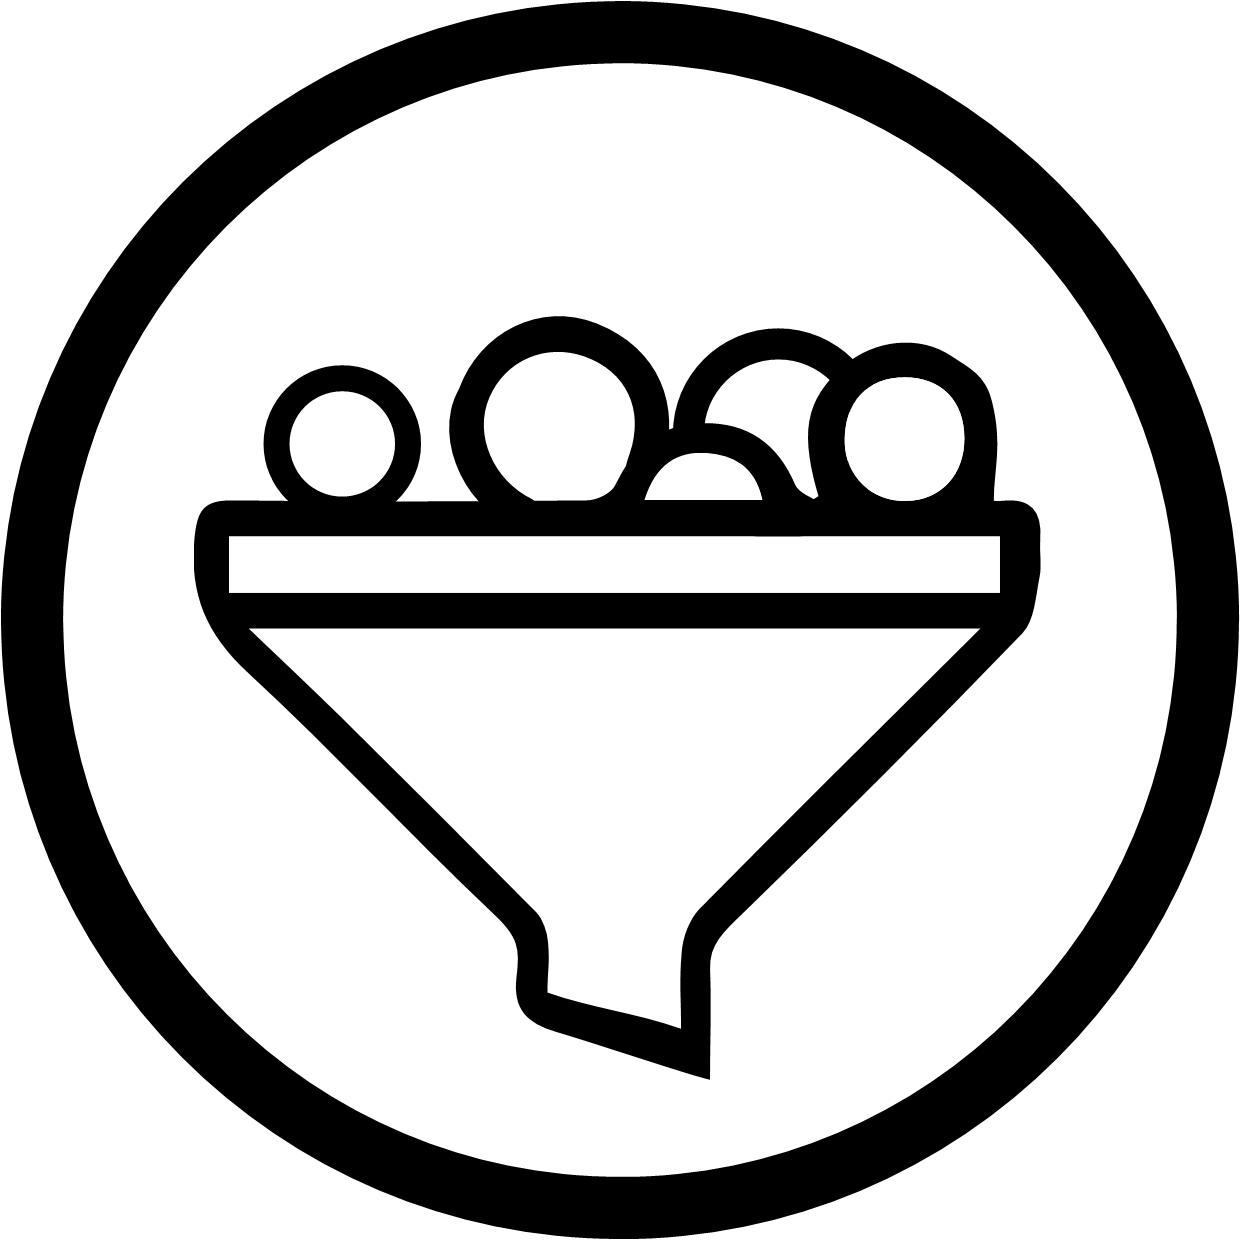
\includegraphics[width=0.1\columnwidth ]{ChapterIntro/Figures/Aggregator.jpg}
	\label{Aggregator}  
\end{wrapfigure}

An aggregator or energy service company (esco) can act as an intermediary between smaller entities (such as consumers) and the market. This is a new role introduced after the deregulation of the electricity market. Aggregators can be seen as local market operators regarding energy and flexibility \cite{Olivella2018}. In terms of flexibility, usually under the concept of a flexibility operator, the aggregator gathers the flexibility provided by DR activities performed by end-users. It can then provide a portfolio based on flexibility services to the TSO, the DSO, and the BRP. An aggregator can also be its BRP, being responsible for its imbalances \cite{VILLAR2018Flexibility}. As a result of this collection and management of DERs, they receive economic incentives. Aggregators are nowadays seen as key actors in the smart grids concept for energy management and therefore flexibility services \cite{Carreiro2017}.\\

\begin{wrapfigure}{l}{1.4cm}
	\centering
	
\includegraphics[width=0.1\columnwidth ]{ChapterIntro/Figures/bill.jpg}
	\label{retailer}  
\end{wrapfigure}


Retailers are existing commercial entities that buy electrical energy from their associated BRP or directly from the market for their customers, assuming BRP responsibilities \cite{VILLAR2018Flexibility}. Within a local electricity market, retailers can broaden their portfolio by including demand-side management (DSM), allowing end-users to receive an incentive for changing their consumption pattern. Retailers can then find a way to compensate for the intermittency of DERs. Furthermore, they can reduce their balancing costs by optimizing their portfolio. \\

\begin{wrapfigure}{l}{1.4cm}
	\centering
	
\includegraphics[width=0.1\columnwidth ]{ChapterIntro/Figures/BRP.jpg}
	\label{BRP}  
\end{wrapfigure}

A balance responsible party (BRP) is a market entity (wholesale supplier, retailer, etc.) that takes up the responsibility to maintain a continuous balance between the energy demand of its customers and the energy bought in the wholesale market or produced directly \cite{mandatova2014flexibility}. A BRP assumes this role by creating a portfolio based on generation and consumption that can be self-provided or exchanged with other BRPs. The goal of BRPs is to minimize the costs of power imbalances whereas aggregators and consumers seek profit maximization \cite{torbaghan2016local}. In addition, they are responsible for balancing demand and supply for a certain metering point. They have to pay penalties for the deviation from their energy forecasting after the energy has been delivered to end consumers. By participating in local and micro markets by providing energy and flexibility services, they can achieve economic savings due to their interaction with aggregators and therefore prosumers. The physical process of generating and consuming electricity is still managed by generators and consumers \cite{KULEnergyInstitute2015}, respectively, and the final responsibility lies with the TSO. Hence, they can be considered administrative entities that are needed within an energy market to ensure this balance.\\


\begin{wrapfigure}{l}{1.4cm}
	\centering
	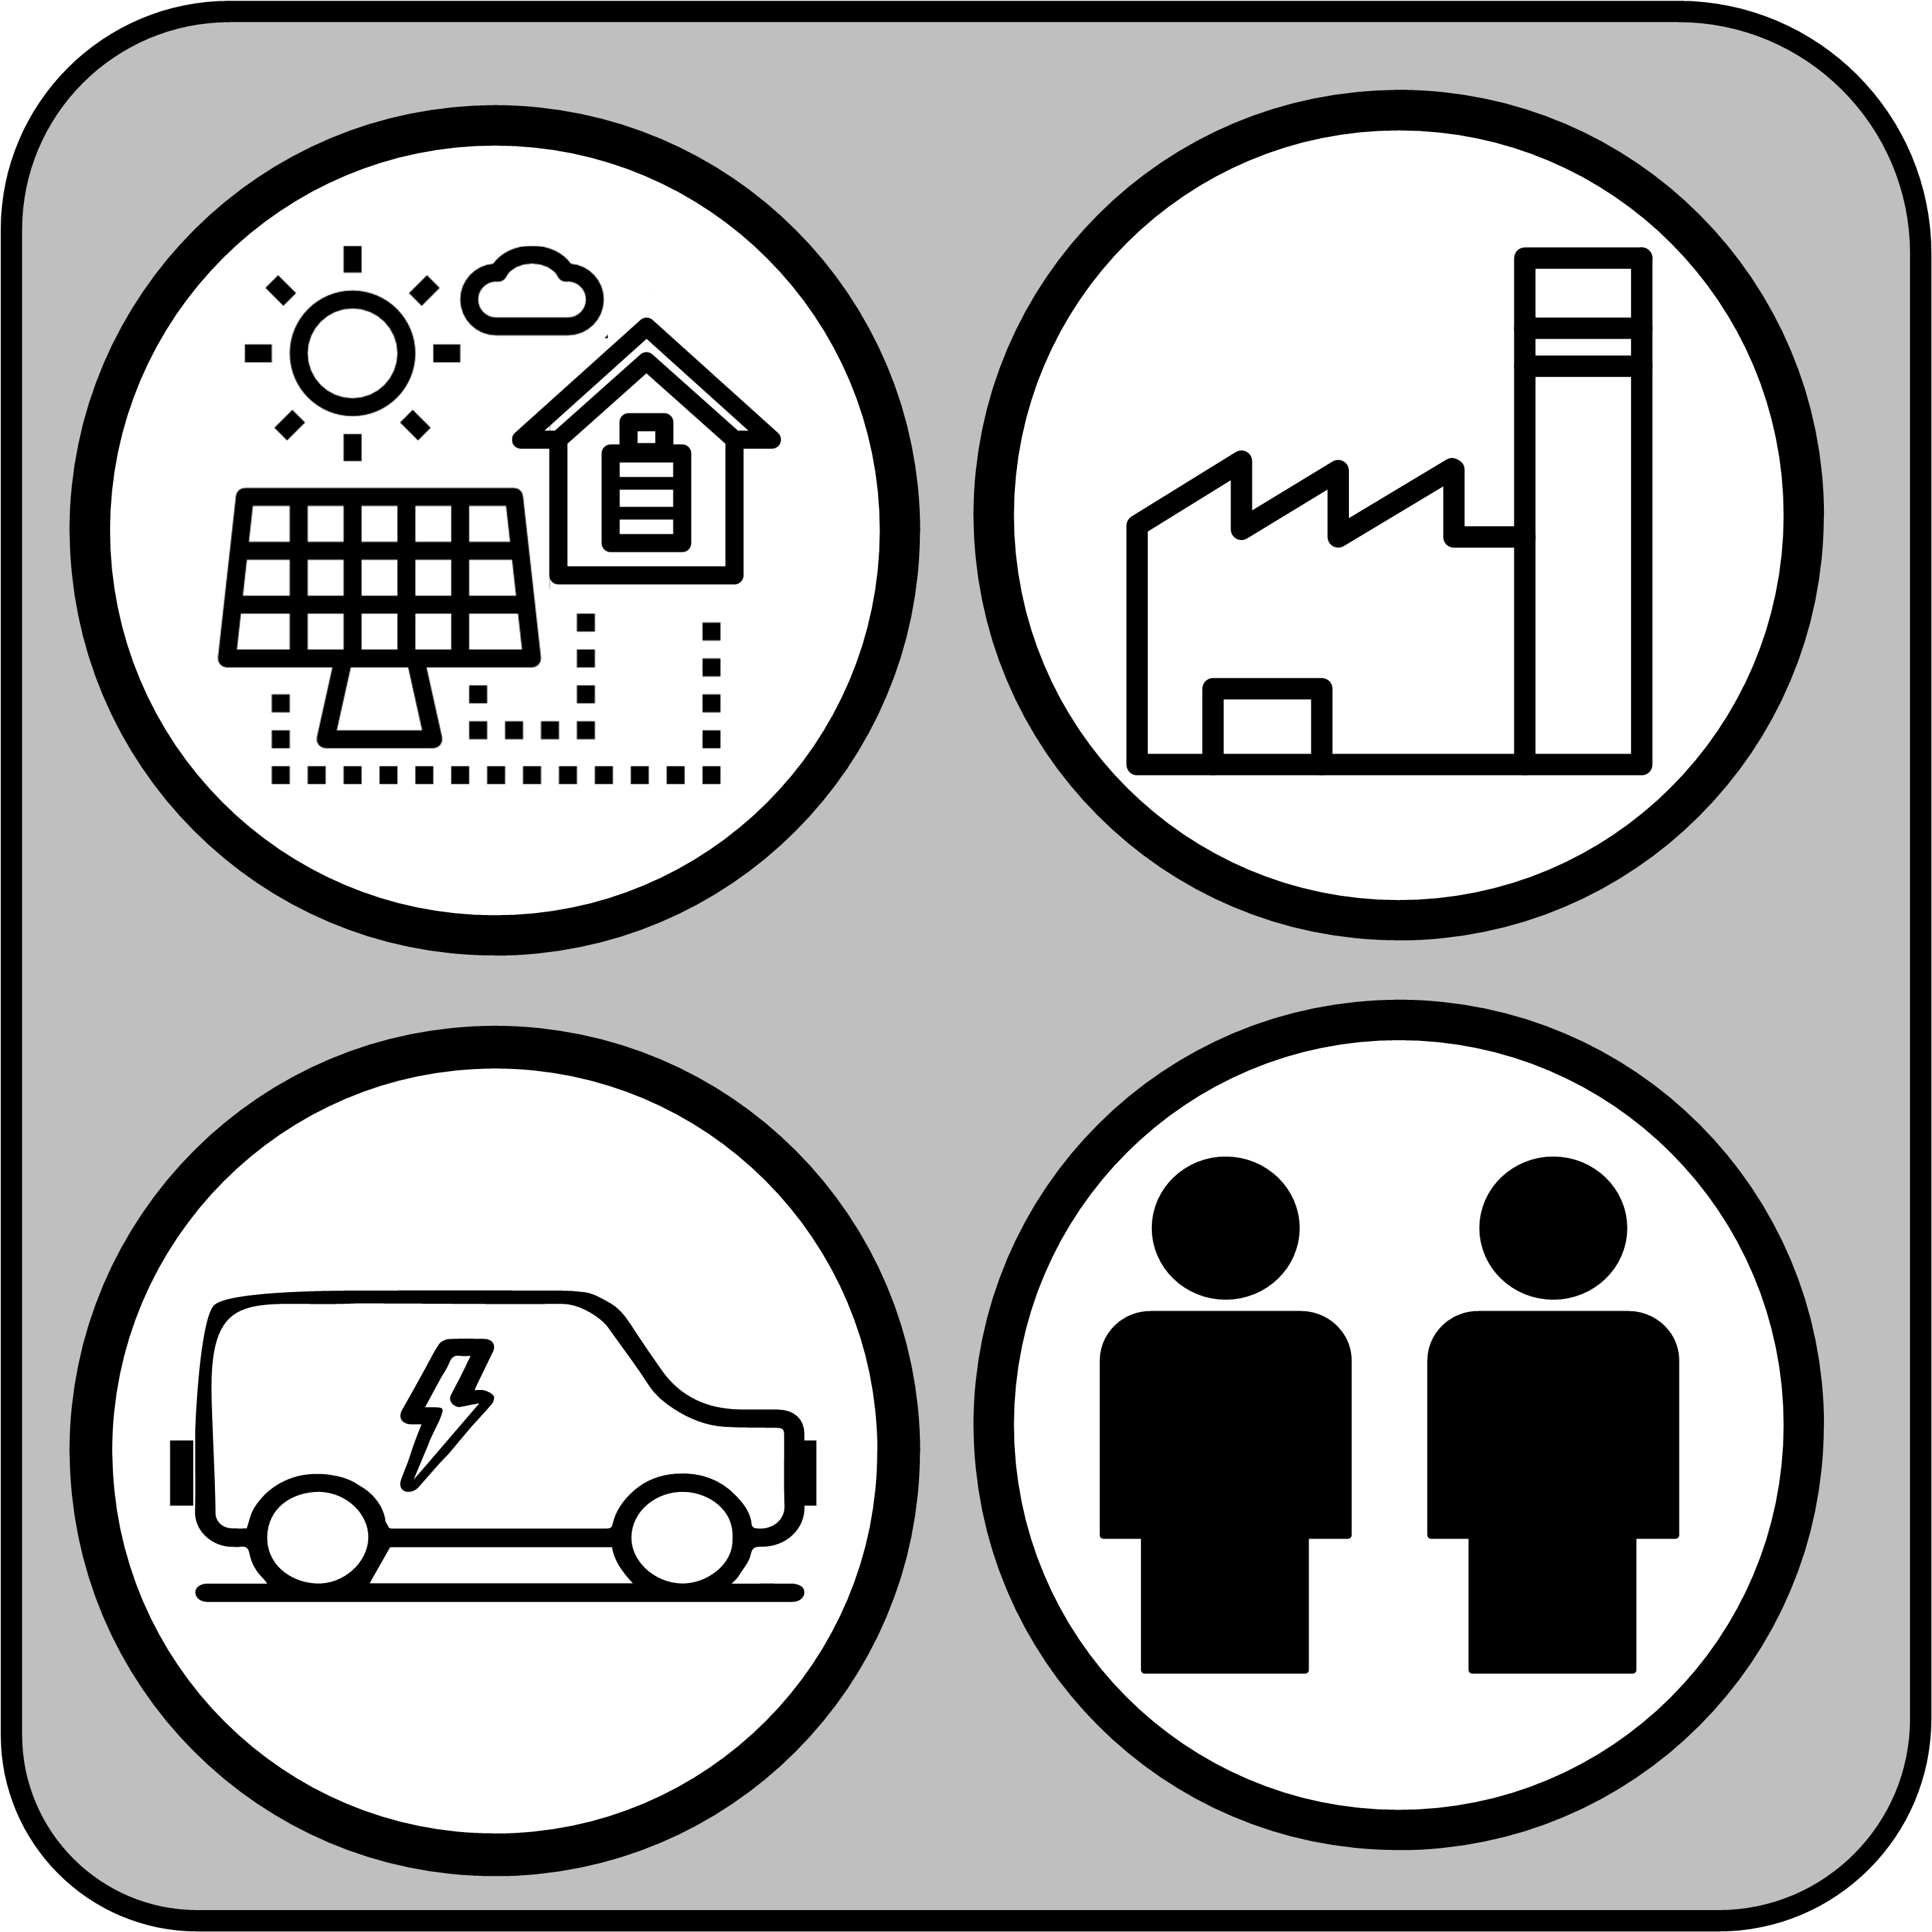
\includegraphics[width=0.1\columnwidth ]{ChapterIntro/Figures/Prosumer.jpg}
	\label{Prosumer}  
\end{wrapfigure}

Prosumers are considered to be active energy consumers that both consume and produce electricity. According to [24], there are four types of prosumers: residential prosumers, citizen-led energy cooperatives, commercial prosumers, and public entities. They consume part of the electricity they have produced by means of the DERs they own and sell the excess to the grid, but they have the capability to buy power from the grid when they require it. They participate actively in energy transition by investing in PV panels or community distributed storage, and so they are evolving from a passive role to a more active role, taking care also of their energy consumption. They are the main energy and flexibility services providers by means of the aggregator figure. As a result, they get incomes for these activities. As stated in \cite{USEFFoundation2015a}, end-users are unaware of the current market structure and have no interest in the market model limitations. However, the current market structure and electricity grid structure present several difficulties for allowing prosumers to buy and sell energy from anyone in the system. Regulatory changes are needed to empower prosumers by creating new services for them. Regarding prosumers and consumers, the concept of active consumers is implanted within the local electricity market terminology. Active consumers are considered to be a group of jointly acting customers who consume, store or sell electricity generated on their premises, including through aggregators, or participate in DSM, DR or energy-efficiency schemes provided that these activities do not constitute their primary activity.\\

\begin{wrapfigure}{l}{1.4cm}
	\centering
	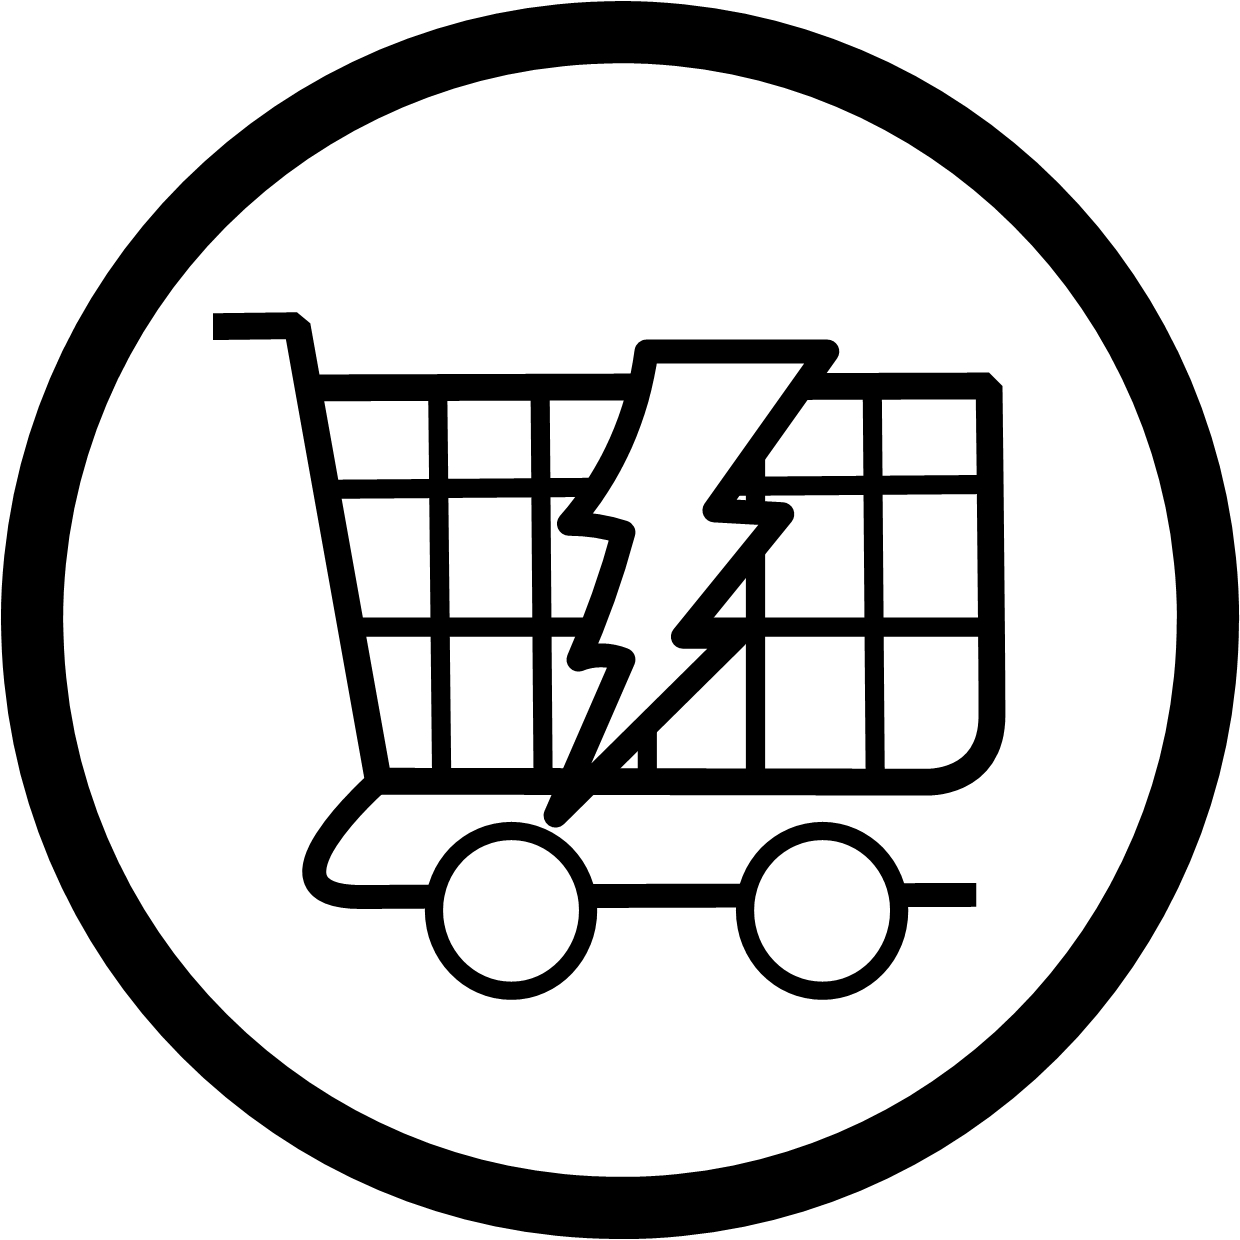
\includegraphics[width=0.1\columnwidth ]{ChapterIntro/Figures/ElectricityMarket.jpg}
	\label{Electricity Market}  
\end{wrapfigure}


Electricity markets are trading places where energy is sold and bought. They are based on two approaches: over-the-counter or bilateral contracts and a pool-based mechanism, which matches the offers and bids and clears the market. Electricity markets are managed by the market operator, which can be different depending on the electricity market itself (day-ahead market [DAM], intraday, forwards, etc.).\\


\begin{wrapfigure}{l}{1.4cm}
	\centering
	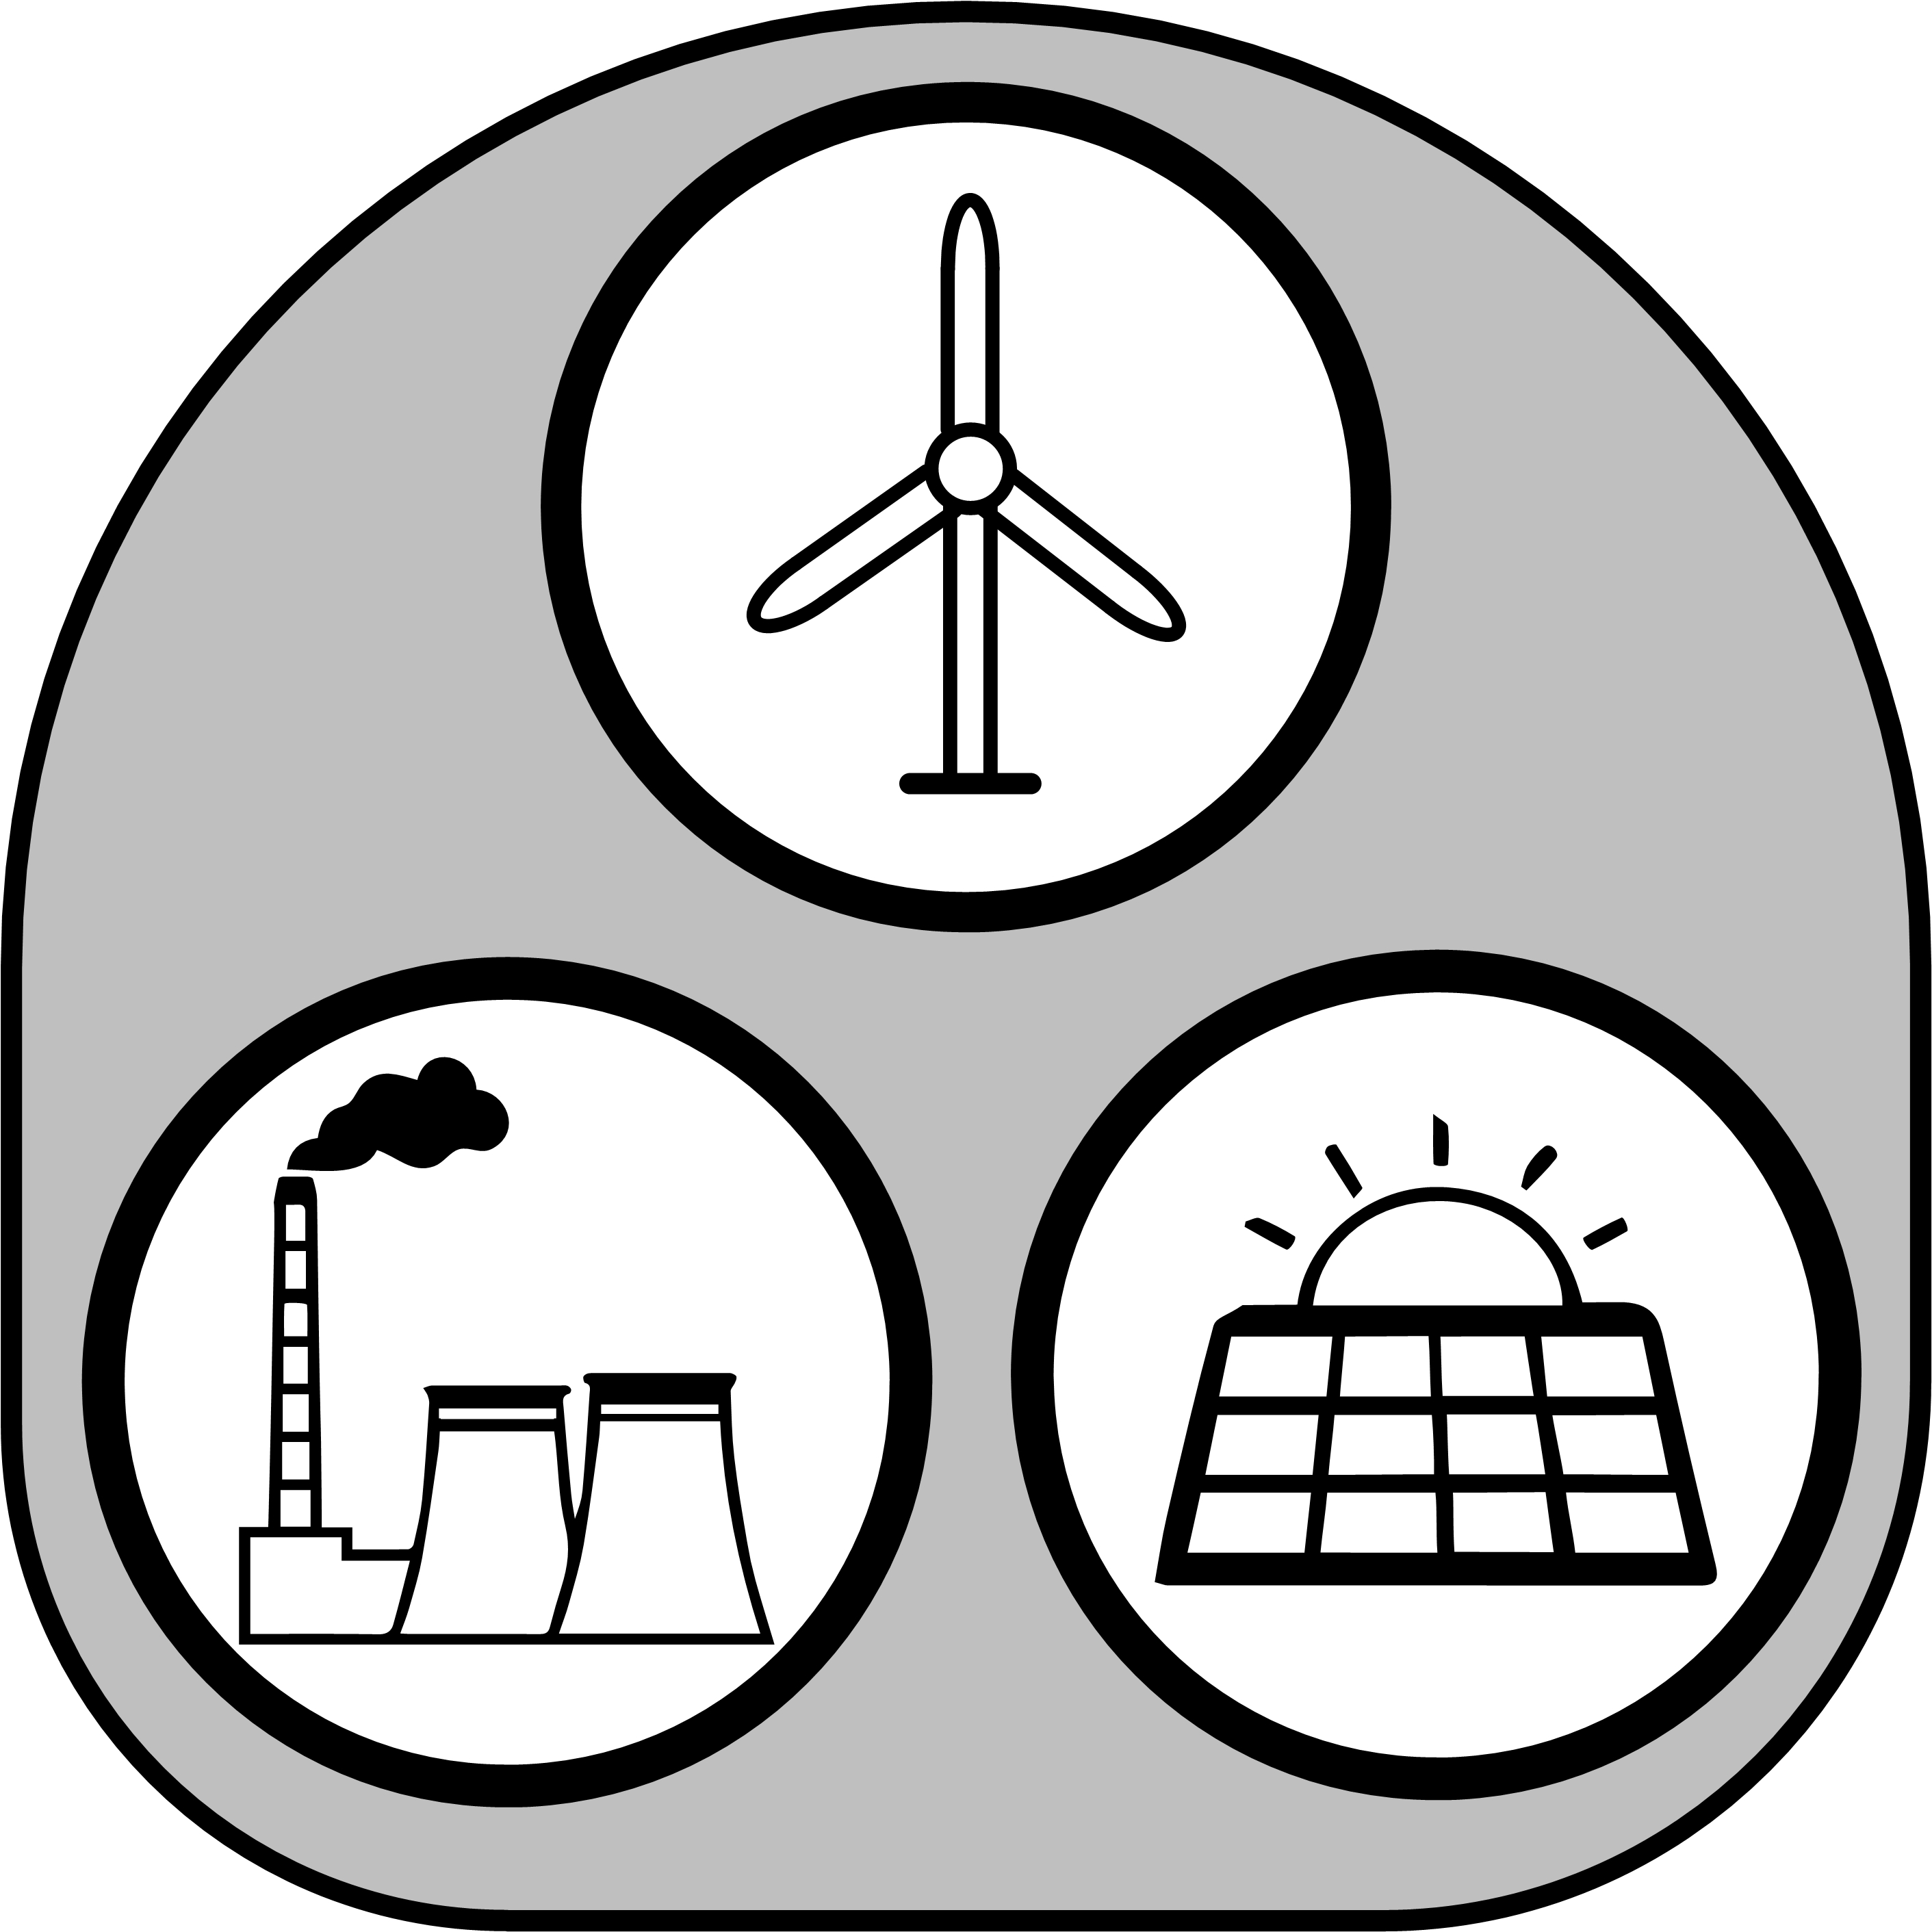
\includegraphics[width=0.1\columnwidth ]{ChapterIntro/Figures/Gencos.jpg}
	\label{gencos}  
\end{wrapfigure}


Generating companies, the so-called gencos or producers, are entities that produce and sell electrical energy \cite{Kirschen2004}. They inject the produced energy into the electrical grid, but also they play a key role in energy supply security \cite{USEFFoundation2015a}. At present, by increasing DERs along the electrical grid, more variability and intermittency has been introduced to the system. However, gencos should guarantee the security of supply regardless of the generation technology.

Once all involved agents have been described, the main benefits for each of them in local market participation can be highlighted.
Table \ref{tab:23} details the main advantages that local market participation can bring to each local market stakeholder. It can be seen that all benefits can be translated into economic value, becoming an incentive or a saving, depending on each local market agent.

% Please add the following required packages to your document preamble:
% \usepackage{booktabs}
% \usepackage{graphicx}
\begin{table}[]
\centering
\caption{Local market stakeholders and main benefit of their interaction}
\label{tab:23}
\resizebox{\textwidth}{!}{%
\begin{tabular}{@{}ll@{}}
\toprule
\textbf{Stakeholder} & \textbf{Main benefits of Local Market Participation}                      \\ \midrule
Prosumer &
  \begin{tabular}[c]{@{}l@{}}Economic incentives for providing energy and flexibility\\ Reduction of energy consumption from the main grid\end{tabular} \\
Aggregator           & Economic incentives for collecting and managing DERs from the demand-side \\
BRP                  & Economic savings due to imbalances penalties reduction                    \\
DSO &
  \begin{tabular}[c]{@{}l@{}}Economic savings by reducing grid investments \\ Operational benefits by avoiding/mitigating distribution network congestions\end{tabular} \\
TSO                  & Operational benefits by providing frequency restoration services          \\ \bottomrule
\end{tabular}%
}
\end{table}

\subsection{Market Approach} \label{sec:marketapproach}

In Section \ref{sec:comparative} the literature review of local and micro power market definitions demonstrated two different
approaches for energy and flexibility exchanges between the involved agents: centralized or pool-based and P2P. Both approaches require the implementation of information and communication technology (ICT) tools as a key factor for local and micro market development and success. This section defines and details the centralized approach and the P2P approach and highlights the main services provided. To start with, Figure \ref{fig:POOL_P2P} represents a schematic view of each trading mechanism, providing an overview of the agents involved in each one. In this section, the main benefits of each approach will be described to give to the reader not only the broad view of each methodology but also the tools and knowledge to research more detailed literature if required. The two approaches are consumer-centric within the LEC and have three main principles \cite{sousa2018peer}:

\begin{enumerate}
\item Agents are willing to share their resources among each other.
\item The grid operation is performed locally instead of being centralized.
\item There is a willingness to self-organize.
\end{enumerate}

The user should notice that, depending on the market design in terms of approach, a different form of offering and clearing algorithm will be applied \cite{Pinson2017}. These two approaches can be seen as extreme approaches. As well as using centralized and P2P approaches in electricity products trading, other end-user focused approaches, such as prosumer-to-interconnected microgrids or prosumer-to-islanded microgrids, as stated in \cite{parag2016electricity}, can also be used. However, these other local and micro market approaches are out of the scope of this chapter.

\subsubsection{Centralized (Pool-Based) Approach}
In a centralized approach, all local market participants need to have a contract with the platform entity who manages the local market services, the so-called local market operator. In this case, direct negotiations or bilateral contracts between traders are not allowed \cite{DesignElectricityMarketRossetoo2017}. Local market or micro market participants in a pool-based approach do not interact with each other directly. The centralized approach offers a unified structure for participant interactions, and it is mainly based on auctions \cite{vytelingum2010trading}. As shown in Figure \ref{fig:POOL_P2P}, the interaction between agents is based on a local market facilitator entity or clearing house, which manages the local resources and coordinates the agents involved in this local market. In a centralized or pool-based approach, there will be a single price for electricity, which means that electricity is a non-differentiable product \cite{Pinson2017}.

In the literature, the centralized approach has been applied to local electricity markets. In \cite{ilieva2016design}, the local market operator is called a smart energy services provider (SESP), which is a platform for energy trading, flexibility trading, information exchange, and actions scheduling. Regarding the technological development of this role, the SESP is usually based on cloud platforms for electricity-related services, such as energy and flexibility. Similar to this approach are the network markets, detailed in \cite{parker2016platform}, where new platforms permit the interaction of new agents within a community. Menniti et al. \cite{menniti2014future} have developed a local market in which a platform facilitator (the city energy provider [CEP]) aims to coordinate the energy exchanges between micro smart grids. 


\begin{figure}[h]
	\centering
	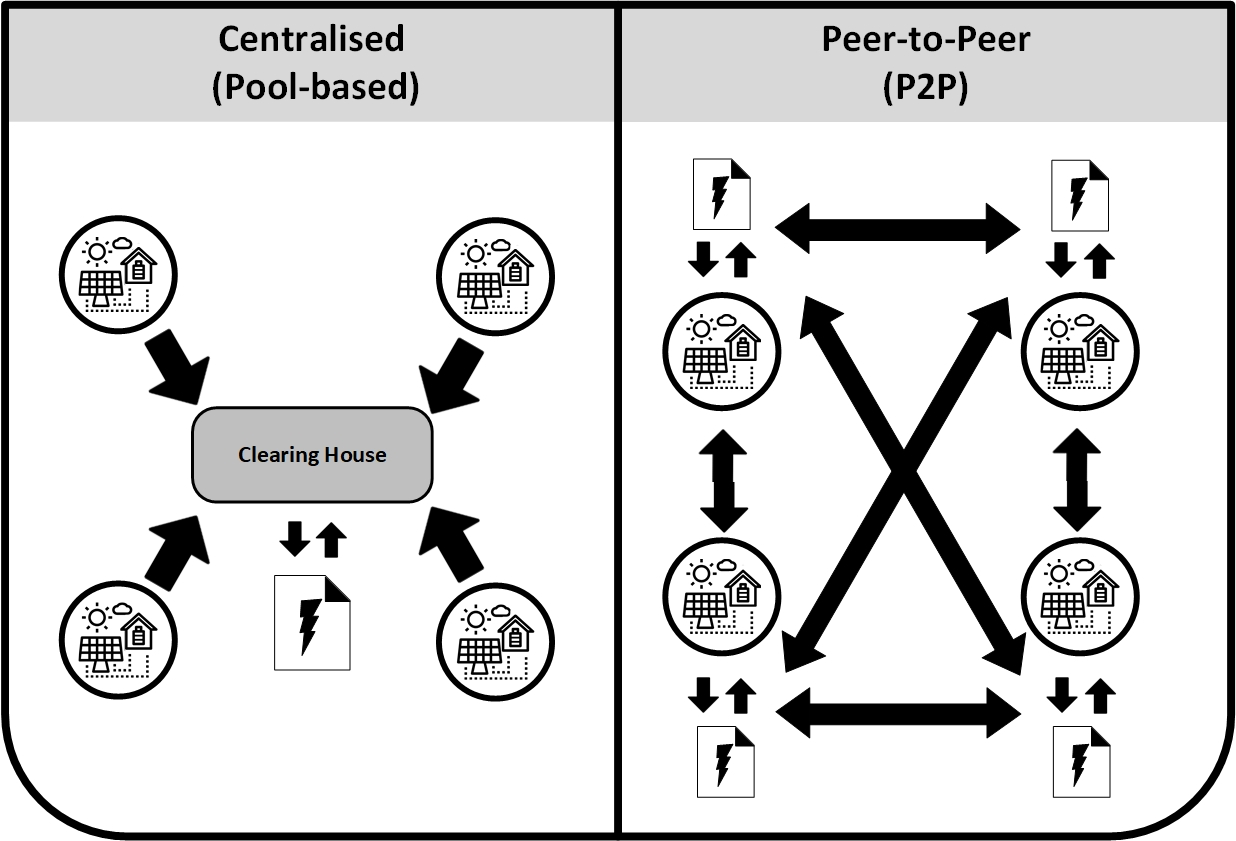
\includegraphics[width=0.7\columnwidth ]{ChapterIntro/Figures/CENTRALISED_P2P.jpg}
	   %\vspace*{-8cm}
		\caption{Centralized vs P2P market approach}
	\label{fig:POOL_P2P}  
\end{figure}

LEMs between prosumers and the DSO can also be developed based on a centralized approach \cite{faqiry2017distributed}. Here, a bilevel iterative auction is proposed and the DSO is the main stakeholder of the market, with aggregators as intermediate agents competing for energy. Nguyen et al. \cite{nguyen2010pool} proposed a new poolbased market platform for flexibility services. The LFM operator is called the DR exchange operator (DRXO), who collects offers and bids and is responsible for the market clearing procedure. In \cite{paschalidis2012demand}, a market-based mechanism was developed based on a centralized approach. The platform operator is the smart microgrid operator (SMO), and it offers regulation service reserves covering the commands issued by the wholesale market independent system operator, which is responsible for energy provision and reserves purchasing. The main participants in an LM operating under a centralized approach are the aggregators, central platforms, the DSO and the group of consumers-producers-prosumers, that is, the LEC members. The LEC members in the LM are recruited from the neighbourhood and organized by the central entity or platform. In that sense, it is important to state that participation in this initiative is purely voluntary. Once the LMs have been broadly implemented in different neighbourhoods, members of the same neighbourhood are able to
choose a different central entity.

Related to the LM participants who are located within the LEC, all members with DERs and flexible loads need to have local control functionalities that can be included in either the smart meter or a local controller to receive command signals from the central entity. This entity also includes communication tools to receive and send control signals and messages between LEC members and the SESP platform, and also to interact with the wholesale market, as will be further detailed in Section \ref{sec:interaction}.

To guarantee a proper development and operation of the LM, each LEC member who participates in the LM is responsible for fulfilling the contract that has been established previously. In that sense, direct negotiations between traders are not allowed. This central entity has a set of roles that should be taken into account to understand the centralized approach. It works as a local market operator, by organizing energy exchange, scheduling local resources, and operating the trading platform. The local market represents the community members when it interacts with the wholesale market. Also, it ensures that all the energy that has been purchased on the wholesale market is consumed by community members and all energy sold must be produced by the LEC. Furthermore, this balance must be constant during all periods, otherwise the central entity will pay deviation penalties. The SESP is responsible for collecting all contracts and offering to their members a brokering, clearing, and price settlement service. The presence of a supervisory node or agent simplifies market regulation and the interface between the local or micro market and the system operator and wholesale market \cite{moret2018energy}.

\subsubsection{Peer-to-peer}
The idea of direct interaction and direct trading between agents in power systems was discussed 20 years ago, in \cite{wu1999coordinated}, where the concept of multilateral bilateral trading was first stated. This is what is now known as peer-to-peer (P2P) electricity trading.

In the P2P approach, prosumers and consumers trade between each other individually and in a randomized order on a pay-as-bid basis \cite{mengelkamp2018blockchain}. In this case, different prices for each trade are possible, since P2P trade involves one-to-one transactions. The P2P approach in energy markets is based on blockchain technology. Blockchain originated in 2008 with Satoshi Nakamoto. Related to blockchain, bitcoin was created in 2009, becoming the first decentralized currency, now known as cryptocurrency. Blockchain can be defined as a distributed and digital transaction technology that allows secure storage of data and execution of smart contracts in P2P networks \cite{swan2015blockchain}. It is a distributed ledger system that instead of having a central entity responsible for coordinating, settling, and archiving, decentralizes this task and relies on a number of entities that work in parallel with a specific ledger copy \cite{Pinson2017}.
In addition, blockchain contains a continuously growing list of data records, which are called blocks. These blocks are time-stamped, shared, unalterable, and connected to preceding blocks. Blockchain blocks can contain data, programs, batches of individual transactions, and executables.

In terms of P2P energy markets, \cite{blouin2001decentralized} proposed a new decentralized market in which there is no auctioneer and transactions take place via pairwise meetings of agents. It could be understood as the first definition of a P2P approach in energy markets. P2P markets rely on a consumer-centric bottom-up approach by giving prosumers the opportunity to choose the energy source they want, based on expressed preferences \cite{sousa2018peer}. The first application of blockchain in electricity markets was developed in 2014 by \cite{mihaylov2014nrgcoin}. These authors proposed a new virtual currency (NRGcoin) for renewable energy trading, which is produced locally. NRGcoins are quite similar to bitcoins. The mechanism converts locally produced renewable energy directly to NRGcoins, independent of their value on the market. Consumption is measured and billed in near real-time, achieving a model that is closed to the current operation of the grid.

Regarding this market approach, few implementations have been developed in the field of energy markets. In \cite{al2015bitcoin}, a new decentralized market for carbon emissions trading based on bitcoin is detailed. Sikorski et al. \cite{sikorski2017blockchain} developed a proof-of-concept to enhance the machine-to-machine electricity market in the chemical industry, also based on blockchain. Related to this market approach, a pilot site based on blockchain as the main ICT was developed in the Brooklyn Microgrid Project \cite{mengelkamp2018designing}. A new architecture for microgrids is presented in \cite{munsing2017blockchains}, where the blockchain P2P approach is applied instead of a microgrid aggregator to manage the DERs within the microgrid. In \cite{mengelkamp2018blockchain}, a double-sided market based on the P2P blockchain approach is detailed. It does not use bitcoin protocol but instead applies the Ethereum protocol. Mannaro et al. \cite{mannaro2017crypto} analysed a blockchainbased software platform for P2P energy trading to enhance renewable energy integration and trading within the Sardinia region. Recently, a project called Enerchain \cite{Enerchain} has been set up to work on P2P energy trading in the wholesale market using blockchain technology. Using this approach for energy trading, the wholesale market operator is no longer needed. This project is comprises energy trading firms that take part in the wholesale market at the present time. The evolution of the power system leads to new market design, business models, and market approaches, and the path leads towards a fully decentralized power system, with different scenarios still opened. To that extent, and based on P2P electricity trading, in theory the power system could be based on consumers being able to choose directly the type of electricity source they want to buy and LECs that provide flexibility services to the system operator or to be traded within the same community. On the other hand, a power system based on LECs could provide a community feeling among the agents involved and trade on energy and flexibility as their main purpose or the energy could also be exchanged with external agents (other microgrids or consumers not located inside the LEC) or with the system operator, for example the DSO. There is a need to define the rules of each smart grid agent to avoid any conflict with the existing top-down power system structure, wholesale market, and additional electricity markets.


\subsection{Services} \label{sec:services}
The main aim of local electricity markets is to facilitate the transition towards a smart energy grid by connecting new or redefined smart grid agents thanks to new services provision. In this chapter, the literature review has introduced two different services that can be provided by a local market: energy trading and flexibility services exchange. These services can be provided separately or together between local market agents 

\subsubsection{Energy}
Most of the literature references we have found defined LEM for energy trading. According to \cite{ilieva2016design}, the objective of the energy service is to schedule local resources at minimum cost during the day ahead, achieving an equilibrium point between local demand, local supply, and grid exchange. First, an energy service is a way to sell and/or buy energy for customer purposes. The main concept to take from the local market for energy services is trading energy locally (from local resources inside the LEC) to reduce electricity consumption from the main grid.

Two LEM approaches are detailed in \cite{mengelkamp2018blockchain}: the P2P market and the closed order book market, with the aim of trading electricity directly within their community and concluding that the P2P LEM approach is the most advantageous, with the lowest energy prices. Later, in \cite{mengelkamp2017role}, a LEM case study based on P2P trading and bitcoin, without the need of central intermediaries, was developed. In this work a framework is also described, with seven market components for its efficient performance. Energy trading within a microgrid based on a P2P approach was developed in \cite{luo2014autonomous} to minimize the microgrid operation cost by increasing the integration of renewable DERs. In \cite{menniti2014future}, a new market platform was created to coordinate energy exchanges between micro-smart grids aggregated in a virtual energy district (VED). It is based on a centralized approach and the local market operator, the CEP, handles the supply and demand of prosumers within the VED. In \cite{Menniti2015}, the integration of distributed energy storage within the VED is analysed to improve the performance of the LEM.
Cui et al. \cite{cui2014electricity} considered a microgrid as a closed economy group and detail two market-based approaches. The first model deals with the optimal power generation per hour within the microgrid. The second model allows energy trading between microgrids for local welfare maximization.

Interactions and power exchanges between microgrids can also be considered as microgrid energy markets or micro markets. In \cite{Lee2015, Gregoratti2015}, market-based mechanisms are studied to schedule and exchange power flows between microgrids, to minimize the global operation cost. In \cite{ferruzzi2016optimal}, a prosumer acts as an aggregator within the microgrid and buys or sells the energy in the DAM. This paper considers the uncertainty provided by the DERs located within the microgrid. Cintuglu et al. \cite{cintuglu2015real} implemented a multiagent-based game theory auction market model that combines conventional and renewable DERs to schedule the microgrid resources. Staudt et al. \cite{staudt2017analysis} defined an LEM as a market set up to solve redispatch locally by providing economic incentives for the expansion of local capacity generation.
Prosumer clustering is a topic that is currently being addressed in the literature \cite{doulamis2017virtual, vergados2016prosumer, da2013impact}. This approach can enhance prosumer participation in local and micro energy markets. Prosumer clustering is an aggregation of prosumers through ICT platforms.
At a higher level, coordination of micro and local markets can also be considered as a local market \cite{menniti2014future}.

This new market aims to coordinate the energy exchanges between local and micro power markets. In \cite{zachar2016microgrid}, microgrid interaction with the macrogrid or distribution network is defined in a market-based approach. 
Storage and community energy storage (CES) are key elements in local and micro energy markets to achieve the optimal operation of the energy market and DERs located within the LEC \cite{Olivella2016ENERGYCON, Bayram2014, mengelkamp2017role, Menniti2015, menniti2014management, mediwaththe2017competitive}. Storage can be understood as units that are controlled by the local market operator to maximize the social welfare of the LEC \cite{Olivella2016ENERGYCON}. Results in \cite{mengelkamp2017role} indicate that LECs with CES have greater local market efficiency. 

The scheme in Figure \ref{fig:marketinteraction} exemplifies how an LEM can work. The LEC is represented by the grouping of different prosumers. This LEC can trade locally by means of an LEM operated by a local market operator or the aggregator. The LEM schedules the local resources depending on their market time horizon, usually the day-ahead. Then, if there is a surplus or a lack of energy resources based on the LEC's resources, the LEM can interact with the day-ahead wholesale market or intraday market to trade the energy needs.


\begin{figure}[]
	\centering
	\includegraphics[width=1\columnwidth ]{ChapterIntro/Figures/Figure2.8.jpg}
	   %\vspace*{-8cm}
		\caption{Local energy market interaction}  
	\label{fig:marketinteraction}
\end{figure}


\subsubsection{Flexibility}
Flexibility can be understood as DR or DSM activities, the so-called demand-side participation. As DERs are installed along the distribution grid, there is a need for end-user flexibility to maximize DER integration and their profitability. In addition, high flexibility is required to deal with the uncertainty of renewable generation and variability on the demand-side. An electric flexibility service can be defined as a power adjustment sustained at a given moment for a given duration from a specific location within the network \cite{Lee2015}. Flexibility activities reflect the possibility of modifying generation and/or consumption patterns in reaction to an external signal (price or activation) to contribute to the power system stability cost-effectively \cite{VILLAR2018Flexibility}. DR is considered to be the tool that will be used to achieve energy efficiency and intermittent RES goals, and where customers will play a crucial role. Thus, according to the previous definition, there are three types of DR actions, according to Albadi and El-Saldani \cite{albadi2008summary}:

\begin{itemize}
\item Electricity reduction. End-users reduce their electricity usage during critical peak periods when prices are
high, but they do not change their consumption pattern. This leads to temporary comfort losses. 
\item Load shifting. Consumers shift their consumption activities from peak demand periods to off-peak periods to respond to high electricity prices. To exemplify this, end-users shift their household activities (dishwashers, washing machines, electric vehicle (EV) charging) to lower-priced periods. In this case, there is no or little reduction of comfort. 
\item On-site generation. Consumers who generate their power by using DERs can follow their consumption profile without changing their behaviour, but by just swapping the origin of the electricity generation. In this case, they experience no or little change in their load profile but, from the utility point of view, a reduction of energy consumption will be noticed.
\end{itemize}

To sum up the characteristics of DSM and DR, Figure \ref{fig:2.9} collects the different tools under the ideas of DSM and DR. Here, DR is considered to be a type of DSM where a temporary reduction or increase in energy consumption is performed by the end-user. Energy efficiency is also grouped under DSM. In this case, energy efficiency covers all the measures or investments performed to achieve lower energy consumption.

\begin{figure}[]
	\centering
	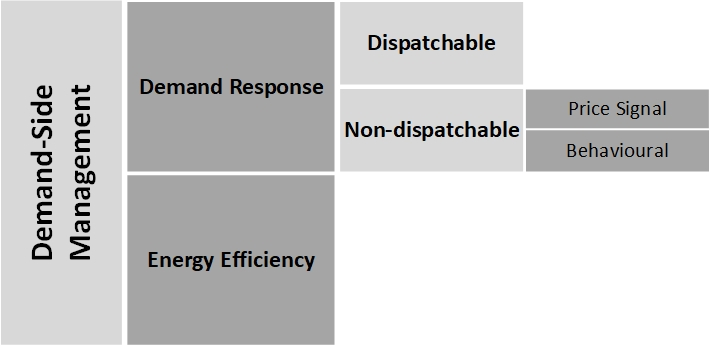
\includegraphics[width=0.8\columnwidth ]{ChapterIntro/Figures/DRDSM_BW.jpg}
	   %\vspace*{-8cm}
		\caption{Demand-Response and Demand-Side Management activities classification} 
	\label{fig:2.9}
\end{figure}

There are two types of DR: dispatchable and non-dispatchable. According to \cite{DNVGLEnergy2014}, dispatchable DR (DDR) refers to \textit{"planned changes in consumption that the customer agrees to make in response to a requirement from someone other than the customer. It includes direct load control of customer appliances and a variety of wholesale programs offered by RTOs/ISOs that compensate participants who reduce demand when directed for either reliability or economic reasons"}. For that reason, DDR can be considered as the participant giving the control of the loads to the utility, who is in charge of its management depending on the needs. Hence, dispatchable DR can be understood as direct control classical incentive-based programs in the DR classification defined in \cite{albadi2008summary}.

In non-dispatchable DR, participants choose if they want to change their behaviour. The utility sends information to the participant and it is the end-user who decides whether or not they follow the signal. Here, the participant remains the master of his loads and consumption. Two programs are included under nondispatchable DR: price-signal and behavioural. Price-signal is structured in the same way as time of use in a price-based program, where electricity price rates per unit consumption are defined. Behavioural DR is the
most innovative type of DR. ICT tools permitted the creation of this type of DR. Usually, participants in this program receive their energy consumption tracking (behaviour) thanks to smart meters, monitoring, and ICT tools. By using these tools, the participant can predict their energy use, reduce cost and also provide flexibility service to the utility, thanks to energy consumption tracking.
DR has a key role to play in helping to increase electricity system flexibility \cite{Cooke2011}. As a result, it will improve the efficiency of the power system, but also the efficiency of the electricity market and the power system security. A higher penetration of flexibility by DR programs will also help the integration of DERs, as DR can help to cover DER intermittency, achieving the goal of carbon footprint reduction (see Figure \ref{fig:2.9}).

The participation of consumers in DR activities can set up a proper market design to integrate flexibility services and increase market competition \cite{MarketDesignENTSOE}. Local flexibility services for the DSO and ancillary services for the TSO at local level can be provided on account of DER integration \cite{Roques2017}.

As a result of DSM and, more specifically, DR activities, flexibility comes into play. Flexibility can be used to adjust the demand profiles during peak periods, to adjust them to peaks of renewable generation, and, related to that, to the available capacity in the distribution grid.

A new framework to create markets for flexibility services has been defined in \cite{Ulbig2015,USEFFoundation2015a}: 'Demand response through load shifting and the storage and management of locally generated energy provides new means to unlock flexibility in the energy system'. In order to provide services to the power system operators, for instance the TSO or DSO, flexible resources and DERs are considered a group, facilitating their operability for flexibility services providing. The aggregator is then a key agent to add value to flexibility. It is responsible for aggregating the prosumers' flexibility, creating a flexibility portfolio and offering it to different stakeholders by means of diverse markets. The aggregator can then also offer services as a supplier and assume BRP responsibilities \cite{MarketDesignENTSOE}. Eurelectric states in \cite{mandatova2014flexibility} that there is a need for a new agent in the system, the flexibility operator and flexibility platform, which aggregates and coordinates the activation of flexible loads located along the distribution network. This market platform should facilitate coordination between the TSO and DSO, and minimize the cost of flexibility market participation. However, the impact of flexibility load participation in the market has to be analysed because it can lead to congestion in the distribution grid \cite{esterl2016impact}. The role of aggregators in DR programs is relevant in involving end-users in smart grid transition and providing ancillary services to system operators, both the TSO and the DSO \cite{Carreiro2017}.

Also in \cite{USEFFoundation2015a}, four potential customers are identified (Figure \ref{figure210}): the prosumer, the BRP, the DSO, and the TSO, managed by the aggregator as a central entity. Up to now, local markets for flexibility services have been mainly based on a centralized approach (Table \ref{tab:23}).

\begin{figure}[h]
	\centering
	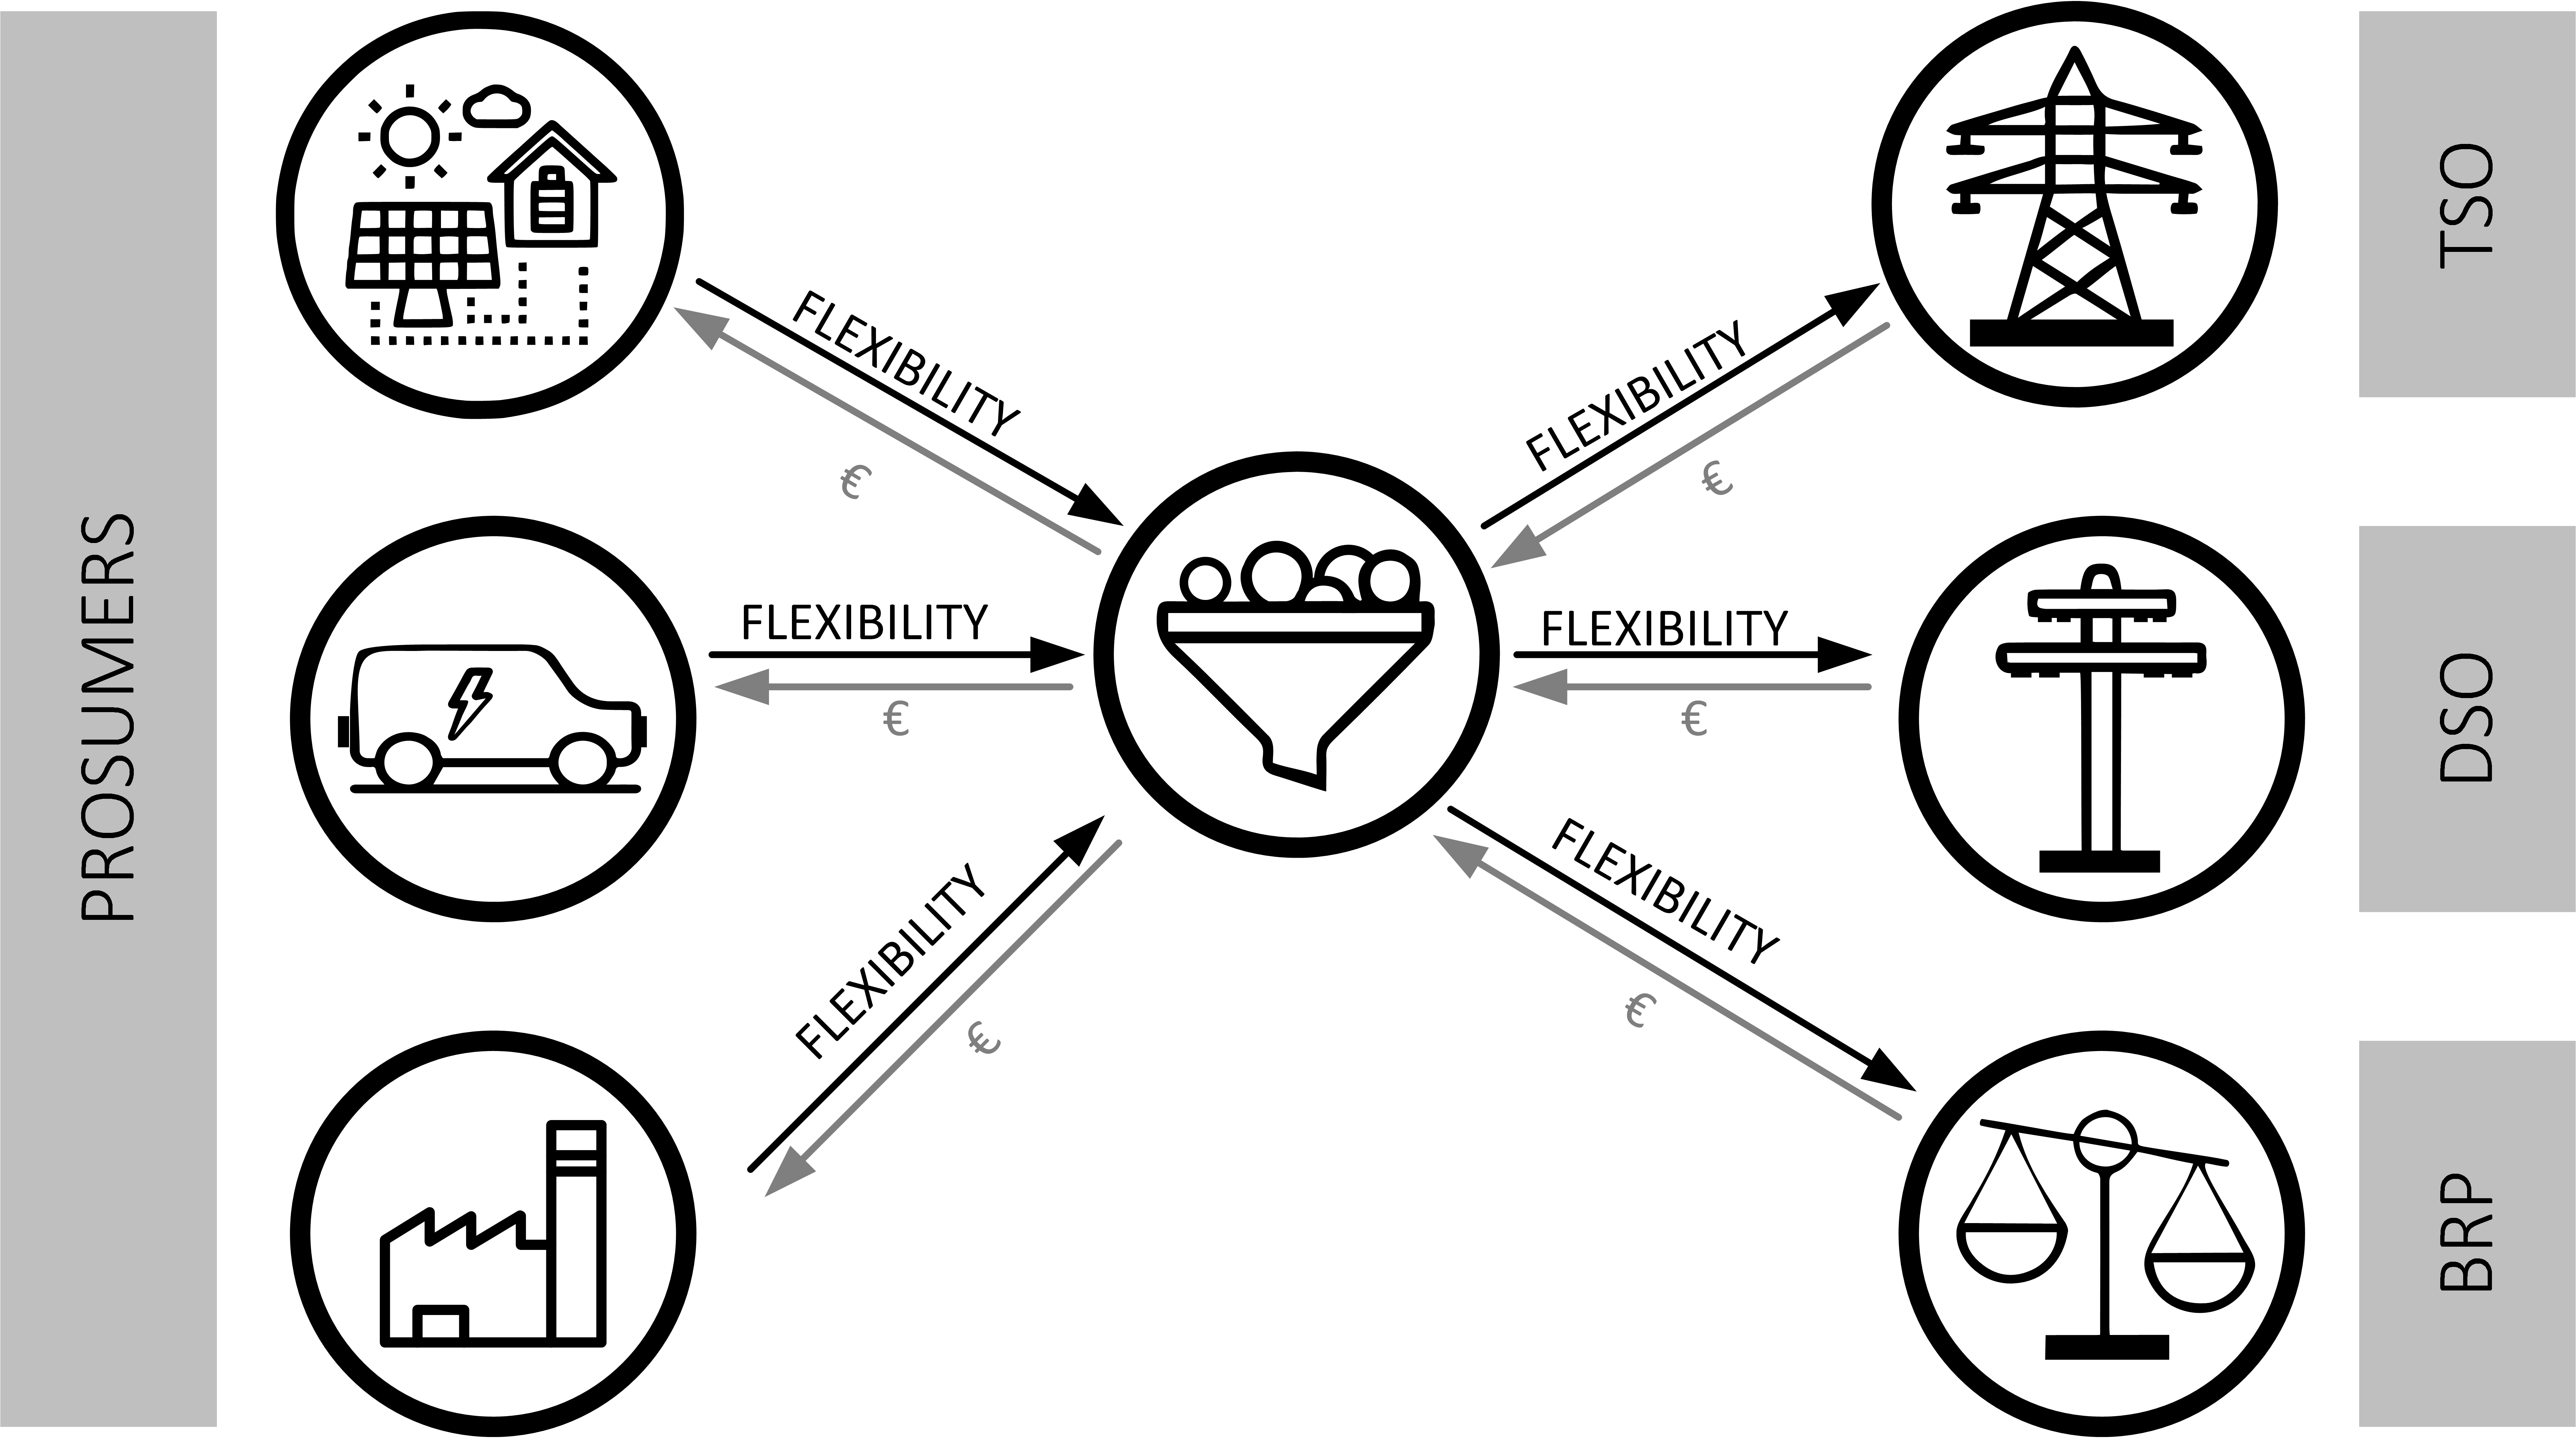
\includegraphics[width=0.9\columnwidth ]{ChapterIntro/Figures/Figure2.10.jpg}
	   %\vspace*{-8cm}
		\caption{Flexibility services and main stakeholders. Figure based on \cite{USEFFoundation2015a} }  
	\label{figure210}
\end{figure}

The market models proposed in \cite{USEFFoundation2015a, MarketDesignENTSOE} do not have an effect on the energy supply chain. They respect the European liberalized energy market model, but change the roles of the involved agents (Section \ref{sec:agents}) for these new services to be provided. The aggregator establishes a smart contract with the prosumer, optimizing the flexibility value in its portfolio and selling this flexibility to the stakeholder with the highest need for this service who is also willing to pay the highest price for it. It should be taken into account that here the role of the aggregator can be developed by a supplier or by an independent aggregator. In any case, they can take BRP responsibility or not.

Recently, several associations, such as Eurelectric, Groupement Europ\'{e}en des entreprises et Organismes de Distribution d'Energie (GEODE), the European Distribution System Operators Association for Smart Grids (EDSO for Smart Grids), and the European Federation of Local Energy Companies (CEDEC), have produced a report focused on the development of flexibility services for the DSO \cite{edso2018flexibility}. This report highlights the need for an improved regulatory framework that rewards the use of flexibility and also takes into account the evolving role of the DSO as an active system operator and neutral market facilitator. DSOs should be able to decide on the best solution to face challenges, either by activating flexibility services or by network reinforcement.

Figure \ref{fig:211} shows the entire supply chain with flexibility services integrated. At the top of the figure, the top line represents the energy flow from the generation plant to the transmission network, the distribution network and arriving at the consumers. Prosumers can also inject their small-scale generated power into the distribution network if regulation allows them to do that. As can be seen in the figure, the energy supply chain remains unalterable with the integration of flexibility services.

\begin{figure}[h]
	\centering
	\includegraphics[width=0.9\columnwidth ]{ChapterIntro/Figures/Figure2.11.jpg}
	   %\vspace*{-8cm}
		\caption{Flexibility services in a local flexibility market. Scheme and interaction}  
	\label{fig:211}
\end{figure}

The ticker line in the middle represents the flexibility flow. The aggregator settles a smart contract with the prosumer. This contract states the terms and conditions of the contracted flexibility services. Hence, the aggregator collects all the smart contracts, optimizes the flexibility assets portfolio, and then offers this flexibility to different stakeholders: the DSO, the BRP, and the TSO by means of the BRP. 

Lastly, the line at the bottom of the figure represents the economic flow between the different agents of the smart grid that combine energy and flexibility flows. The economical flow takes into account that the energy is sold and bought on electricity markets. The BRP is the entity responsible for the imbalances that are paid after the actual delivery. As a result, retailers, by means of the energy bill, are paid for the energy delivery to end-users. Furthermore, the BRP applies the imbalance payment to the final bill that the end-user is disbursing.

Current literature proposes different services offered by LFMs or local markets for flexibility services. Olivella-Rosell et al. \cite{Olivella2018} developed an LFM. In this the local market operator controls the LEC flexible resources (thermal loads, EVs, storage, etc.) during specific time periods and rewards the participants accordingly on their smart contracts. On the contrary, LFM can be understood as a trading platform to adjust the energy resources to correct forecasting errors or to increase the participant's profits in balancing markets \cite{ilieva2016design}. In \cite{diekerhof2017hierarchical}, an aggregator collects and optimizes the day-ahead and intraday scheduling of electro-thermal heating units within a city district to provide flexibility services to the DSO and BRPs. Ramos et al. \cite{ramos2016realizing} described three different local market designs for local flexibility services for DSO: participating in the existing wholesale market, creating an LFM, and contracting flexibility as a system reserve. Bilateral contracts for flexibility services based on thermal loads from residential DR are defined in \cite{boscan2016flexibility}. The optimization model is also detailed and presented in \cite{boscan2016flexibility}, taking into account consumer preferences so that end-users can select their own contract based on them. Specific topics directly related to flexibility services are currently addressed in the literature, such as aggregating flexible loads \cite{nayyar2013aggregate, pandvzic2013offering} and thermostatic loads \cite{alahaivala2017control}.

In \cite{leclercq2019network}, flexibility market-based schemes are defined for TSO-DSO coordination. Two LEMs are detailed: a local AS real-time market and a common TSO-DSO AS market model. The local AS real-time market considers balancing and congestion management services for the DSO and the TSO. The DSO operates the local market to solve distribution grid problems and then aggregates the remaining flexibility offers to the TSO markets. 

The TSO-DSO AS market model is also based on real-time dispatching. It is based in a local market operated by the DSO, but satisfies the needs for both the TSO and the DSO. The LFM can be established to provide flexibility services to the TSO. Teotia and Bhakar \cite{teotia2016local} defined the local electricity market concept as an ancillary services provider for the DSO and TSO by creating a new local market operator, an aggregator, and a local grid controller (LGC). The LGC is responsible for the management of the local grid resources, such as energy storage, combined heat and power, residential flexible loads, and DERs. In \cite{rosen2013auction}, an auction-based LEM for TSO ancillary services trading is detailed based on BRP enhancement. Also related to ancillary services, \cite{martinez2013active} developed a secondary market for ancillary services offered by active demand participation (prosumers) to minimize grid operation costs. Regarding ancillary services, \cite{menniti2014future} considers them as a possible service that the LEM could provide to the TSO and DSO.

Different projects and market designs for electric flexibility trading are reviewed in \cite{eid2016market}. First, the Power Matching City project developed a local market operator, Powermatcher, which is in charge of controlling the operation of household appliances located in the Netherlands by means of direct and semi-direct control. 
The flexibility services are offered by prosumers to the DSO and retailers. The Energy Frontrunners project developed a flexibility aggregator that acts as an intermediary between the flexible loads, the BRP, and the DSO. In this project, the aim of the flexibility trading is to reduce the PV panels' peak and so the peak load in the distribution network during the evening period. In Germany a local integrated utility is at the same time the retailer, the owner of the distribution network, and also acts as a flexibility operator. It is responsible for trading flexibility between the TSO and the utility that controls the flexible loads. Here there is no participation of the DSO, the retailer, and the prosumers; the local integrated utility controls the operation of these flexible
loads and also of the grid.

A P2P approach can also be used in LFM, but it is not widely applied. Chen et al. \cite{chen2017integrated} proposed a new market mechanism for EV parking lots to participate in real-time markets, based on smart contracts and a P2P approach. These flexible loads can adjust their demand and consumption behaviour according to DSO requirements and incentives. The Your Energy Moment project \cite{eid2016market}, also developed in the Netherlands, is based on dynamic pricing signals that consumers receive thanks to in-home applications. Both the DSO and the retailer are able to submit their price to the participant.

\section{Local Market Services and Approach Review} \label{sec:servicesreview}
As a summary of the literature review detailed before, Table \ref{table24} shows the published papers in terms of the services provided, the main stakeholder, and the market approach. This table aims to show an overview of the current status of local and micro power market technology.
%\setlength{\tabcolsep}{10pt} % Default value: 6pt
%\renewcommand{\arraystretch}{1.5} % Default value: 1
%\begin{table}[]
%\centering
%\caption{Local market services and approaches literature review}
%\label{table24}
%\resizebox{\textwidth}{!}{%
%\begin{tabular}{@{}lll@{}}
%\toprule
%\textbf{Service / Approach}           & \textbf{Peer-to-peer} & \textbf{Centralized} \\ \midrule
%\textbf{Energy}                       &  \cite{mengelkamp2018designing, sousa2018peer, lamparter2010agent, vytelingum2010trading, moret2018energy, Heidari2018, Bayram2014, Pinson2017, mihaylov2014nrgcoin, munsing2017blockchains,mannaro2017crypto, Enerchain, mengelkamp2017trading, long2017feasibility, pouttu2017p2p, sorin2018consensus, baroche2018exogenous}  &                    \cite{sousa2018peer, karnouskos2011demand, rosen2013auction, ampatzis2014local, menniti2014local, EuropeanNetworkofTransmissionSystemOperatorsforElectricityENTSO-E2015, ilieva2016design, staudt2017analysis, moret2018energy, menniti2014future, cui2014electricity,     shamsi2015economic, Bayram2014,Pinson2017, faqiry2017distributed, Menniti2015, Lee2015,Gregoratti2015, ferruzzi2016optimal, mediwaththe2017competitive, mengelkamp2017trading, holtschulte2017local, wu2015optimal, mohan2015online, mohan2016sortino, gui2017distributed,lezama2018local}   \\
%\textbf{Flexibility to TSOs}          &  -                     & \cite{nguyen2010pool, nordentoft2013development, rosen2013auction, ramos2016realizing, leclercq2019network, staudt2017analysis, USEFFoundation2015a, martinez2013active, eid2016market, olek2014local}                      \\
%\textbf{Flexibility to DSOs}          & \cite{eid2016market, chen2017integrated, kok2016society}  &                       \cite{poudineh2014distributed, zhang2014flech, gawron2014integra, zhang2013flex,  spiliotis2016demand, eid2016market, diekerhof2017hierarchical, mandatova2014flexibility, USEFFoundation2015a, Olivella2018, pavlovic2016sgam, leclercq2019network, ramos2016realizing, nordentoft2013development, nguyen2010pool} \\
%\textbf{Flexibility from Demand-Side} &   \cite{eid2016market, chen2017integrated, kok2016society} &                     \cite{validzic2017clean, pavlovic2016sgam, Olivella2018,  USEFFoundation2015a, mediwaththe2017competitive, eid2016market,  mohan2015online,  lezama2018local,  gawron2014integra, zhang2013flex, spiliotis2016demand, zhang2014flech} \\
%\textbf{Flexibility to BRPs}          &   \cite{eid2016market} &   \cite{validzic2017clean, nguyen2010pool, pavlovic2016sgam, Olivella2018, USEFFoundation2015a, diekerhof2017hierarchical, eid2016market, zhang2013flex}                       \\ \bottomrule
%\end{tabular}%
%}
%\end{table}

\begin{table}[h]
\centering
\caption{Local market services and approaches review}
\label{tab:24}
\resizebox{\textwidth}{!}{%
\begin{tabular}{@{}lll@{}}
\toprule
Service / Approach &
  Peer-to-peer &
  Centralized \\ \midrule
Energy &
  \begin{tabular}[c]{@{}l@{}}\cite{mengelkamp2018designing, sousa2018peer, lamparter2010agent, vytelingum2010trading, moret2018energy, Heidari2018, Bayram2014, Pinson2017, mihaylov2014nrgcoin}\\ \cite{munsing2017blockchains,mannaro2017crypto, Enerchain, mengelkamp2017trading, long2017feasibility, pouttu2017p2p, sorin2018consensus, baroche2018exogenous}\end{tabular} &
  \begin{tabular}[c]{@{}l@{}}\cite{sousa2018peer, karnouskos2011demand, rosen2013auction, ampatzis2014local, menniti2014local, EuropeanNetworkofTransmissionSystemOperatorsforElectricityENTSO-E2015, ilieva2016design, staudt2017analysis, moret2018energy, menniti2014future, cui2014electricity}\\ \cite{ shamsi2015economic, Bayram2014,Pinson2017, faqiry2017distributed, Menniti2015, Lee2015,Gregoratti2015, ferruzzi2016optimal, mediwaththe2017competitive, mengelkamp2017trading, holtschulte2017local, wu2015optimal, mohan2015online, mohan2016sortino, gui2017distributed,lezama2018local}\end{tabular} \\
Flexibility to TSOs &
  - &
  \cite{nguyen2010pool, nordentoft2013development, rosen2013auction, ramos2016realizing, leclercq2019network, staudt2017analysis, USEFFoundation2015a, martinez2013active, eid2016market, olek2014local} \\
Flexibility to DSOs &
  \cite{eid2016market, chen2017integrated, kok2016society} &
  \begin{tabular}[c]{@{}l@{}}\cite{poudineh2014distributed, zhang2014flech, gawron2014integra, zhang2013flex,  spiliotis2016demand, eid2016market, diekerhof2017hierarchical, mandatova2014flexibility, USEFFoundation2015a, Olivella2018}\\ \cite{pavlovic2016sgam, leclercq2019network, ramos2016realizing, nordentoft2013development, nguyen2010pool}\end{tabular} \\
Flexibility from Demand-Side &
  \cite{eid2016market, chen2017integrated, kok2016society} &
  \begin{tabular}[c]{@{}l@{}}\cite{validzic2017clean, pavlovic2016sgam, Olivella2018,  USEFFoundation2015a, mediwaththe2017competitive, eid2016market,  mohan2015online,  lezama2018local,  gawron2014integra}\\ \cite{zhang2013flex, spiliotis2016demand, zhang2014flech}\end{tabular} \\
Flexibility to BRPs &
  \cite{eid2016market} &
  \cite{validzic2017clean, nguyen2010pool, pavlovic2016sgam, Olivella2018, USEFFoundation2015a, diekerhof2017hierarchical, eid2016market, zhang2013flex} \\ \bottomrule
\end{tabular}%
}
\end{table}

As shown in Table \ref{tab:24}, research has been focused mainly on centralized platforms to deal with local and micro power markets. Furthermore, the main services provided have been energy. For instance, \cite{ilieva2016design} has shown as part of the H2020 project EMPOWER how an LEM can exist side by side with a centralized platform that enables power exchanges. Cui et al. presented a market model for microgrids (micro market) with two different approaches \cite{cui2014electricity}. First, the microgrid is considered as a standalone entity and the central entity schedules the generation for it. The second approach is based on interconnecting close microgrids to trade between them to increase the total welfare, thanks to covering the local demand with local generation. Shamsi et al. solved an economic dispatch (ED) problem for resources scheduling within a microgrid by means of a dynamic ED algorithm for each agent \cite{shamsi2015economic}. It is based on a centralized approach, since there is a microgrid market operator who is responsible for collecting microgrid agents' offers and bids and finding the microgrid spot price. A micro market within a microgrid, using a centralized approach (the microgrid service provider), is theoretically defined in \cite{gui2017distributed}. This central entity is one where community users can acquire the services. It emphasizes the democratic and community feeling on which the microgrid community is based.

In \cite{moret2018energy} an energy collective is presented based on both the P2P and centralized approaches. A community of prosumers is considered, and they are responsible for scheduling their resources using their own priority rules (no social welfare considered of the whole community), that is, behind-the-meter. They can trade the lack or excess of energy by means of a central entity called the community manager. The community manager is also able to directly interact (P2P) with other community managers to trade energy. The community manager is also the smart grid agent who interacts with the market and system operator, as well as being the supervisor of convergence to system optimality. Mengelkamp et al. \cite{mengelkamp2017trading} introduced and compared four scenarios for an LEM. They are based not only on two market approaches, P2P and centralized, but also considering zero intelligence agents and intelligently bidding agents. The research concluded that P2P markets considering intelligent market agents reach a lower average electricity price for the community.

Based on a P2P market approach, in 2014 Mihaylov presented a novel mechanism for energy trading: NRGCoins \cite{mihaylov2014nrgcoin}. They were formulated as a virtual currency for renewable energy injected into the grid, which was later traded between prosumers by means of blockchain technology. Sorin et al. \cite{sorin2018consensus} introduced multilateral energy trading taking into account product differentiation. In this case, the product differentiation covers consumer preferences. It allows prosumers participating in this market to be more involved and proactive due to the possibility of increasing their interest regarding energy origin and typology. One of the drawbacks that is highlighted in this paper and has to be taken into account when working on P2P electricity markets is the scalability of them. The computational costs for scaling a P2P market are higher than for a poolbased market. The latter is considered to be far more structured than P2P trading, thanks to the intermediary that negotiates with the agents involved in the LEC and also to external agents such as the system operator, aggregator, or BRP. A solution proposed in \cite{sorin2018consensus} to increase the scalability of P2P markets is to reduce the communication between agents participating in the market. In order not to rely on any central entity, a blockchain-based microgrid energy market is presented in \cite{munsing2017blockchains}, with the aim of guaranteeing that payments are made between non-trusting microgrid agents. By means of the alternating direction method of multipliers optimization method and local optimal power flow, a set of batteries, and curtailable and shiftable loads located along the distribution grid are scheduled. When dealing with LEMs based on a P2P approach, one of the most important shortcomings is where to allocate the grid costs. Baroche et al. \cite{baroche2018exogenous} present a method to
allocate grid cost based on the electrical distance between market participants. In this approach an ED along with product differentiation is carried out. In many literature papers the ED was done but without taking into account the grid infrastructure.

The fact is that P2P has an impact on the grid status, and the grid status and electrical distance should have an impact on peer interactions. Hence, in this paper, by applying electrical distance cost allocation there is a reduction in power trades between agents because the proposed market mechanism pushes the market agents to consider and respect the power system capacity constraints.
Several projects are currently ongoing in Europe in the field of local and micro energy markets, as stated in \cite{sousa2018peer}, mainly focused on the interaction between prosumers and consumers based on DERs located in a low voltage distribution grid. Local control and ICT platforms are a core part of these projects and both centralized \cite{ilieva2016design} and P2P \cite{moret2018energy, Enerchain, mihaylov2014nrgcoin} approaches are being used to implement the market design.

In terms of flexibility, it is worth separating them into the agents involved in the flexibility services chain. In this case, four distinctions are made: TSO, DSO, BRP, and prosumers. As can be seen from Table \ref{table24}, the centralized approach has also been the main research focus in the field of flexibility services. 

The main actor in receiving flexibility services is the DSO. Due to the increase in DERs and the need for grid capacity enhancement, the DSO needs market tools to facilitate their operation in terms of congestion management. Ramos et al. present three main approaches to contract flexibility: by means of the already existing wholesale market, by creating a new LFM based on a centralized approach, and a reserve market approach, contracting flexibility as a system reserve \cite{ramos2016realizing}. iPower is a project supported by the Danish Government with the aim of innovating and investigating intelligent power. The development of a DSO market for flexibility, by means of DR schemes and based on the aggregator role to collect end-user DR for DSO purposes, is introduced in \cite{nordentoft2013development}. The specifications in terms of flexibility services to be provided by end-users are detailed, such as the size of the service in power, the service in energy, the maximum duration of service per activation, pricing, and penalty. In 2017, another H2020 European project called INVADE began \cite{Olivella2018} with the aim of developing a centralized local flexibility trading platform to sell and buy flexibility within a specific area.

In this platform, the aggregator acts as a central entity and also as an esco. In this project, prosumer flexibility is aggregated by means of the flexibility operator or aggregator, and so it is responsible for participating in the market. This central entity aims to maximize the profits for its prosumer portfolio. Thanks to the flexibility provided by prosumers, the central entity can provide new services to the two main actors in the smart grid: the BRP and the DSO. The use of DR schemes for providing flexibility services to the DSO is analysed in \cite{spiliotis2016demand, poudineh2014distributed} based on a centralized approach.

Flexibility services provided by means of P2P trading are still not implemented as much as the centralized approach. However, Kok et al. \cite{kok2016society} describe a P2P mechanism based on transactive energy to provide flexibility services to the DSO to maintain the distribution network resiliently and efficiently. The mechanism was initially focused on the USA but the PowerMatcher project is ongoing to implement transactive energy trading by giving the consumer and prosumer the role of deciding whether or not to sell flexibility to parties involved in the project. Chen et al. describe a trading mechanism based on P2P to encourage users with flexible loads as EV to adjust their charging behaviour according to DSO requests \cite{chen2017integrated}.

Table \ref{table24} proposes a classification of existing literature in local and micro power markets, considering energy and flexibility as services to be provided and P2P and centralized as approaches to providing these services. This is a topic of current interest and much research is being carried out at present. The roadmap of this technology is evolving from a theoretical framework to even more research and implementation to prove its feasibility. There is still research to be done and questions to be answered, such as the viability of P2P mechanisms for providing flexibility.

\section{Local Market Interaction} \label{sec:interaction}
In this chapter different local market services and structures have been presented. The fact that local markets provide energy and flexibility exchanges may lead to interactions between these new local markets and existing energy markets worldwide. A possible general interaction among these markets is outlined in Figure \ref{fig:212}, based on a centralized approach by a central platform. To run these markets, local traders need this platform for sharing information, trading energy and flexibility, and scheduling actions. The smart energy platform acts as a local market facilitator for the LEC and also as an aggregator for wholesale market agents. The platform takes actions to increase market interactions, ensuring liquidity. Moreover, LMs could have problems balancing consumption and generation using only local resources, in terms of energy. Hence, it is imperative for the central platform to operate in wholesale markets during such periods to buy or sell the community energy deficit or surplus.

\begin{figure}[]
	\centering
	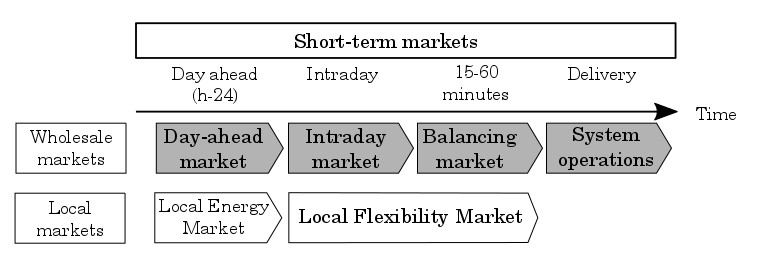
\includegraphics[width=0.9\columnwidth ]{ChapterIntro/Figures/LM_WSM_Interaction.jpg}
	   %\vspace*{-8cm}
		\caption{Wholesale and Local Market interaction in the short term. Based on \cite{InternationalEnergyAgency2016}}
	\label{fig:212}  
\end{figure}


The energy and flexibility LMs have their parallels in the wholesale market. The negotiation period of the LEM is equivalent to the DAM, and the LFM is equivalent to intraday plus the balancing market, as shown in Figure \ref{fig:212}. The reader should take into account that the scheme shown in Figure \ref{fig:212} is one possible option to define the interaction between local and micro power markets and existing wholesale markets. In this chapter we propose an interaction scheme, but there are several options to define the integration between markets. The following chapters examine the different structures. In Chapter 3, specific interactions between micro markets
and wholesale markets are presented and in Chapter 4 the interaction between local markets and wholesale
markets is covered.

As shown in Figure \ref{fig:212}, the first market that is being run or that starts is the LEM. With the aim of maximizing the community benefits for the LEM from the DAM, the central entity asks their members to participate in the LEM. It starts one day before the delivery or operation day, and the central entity estimates local energy consumption to determine if the LEC has to purchase or sell electricity in the DAM. The SESP prepares bids and offers for the DAM with the objective of minimizing energy costs. In addition, this central entity also is able to schedule flexible loads to reduce energy costs or, on the contrary, maximize LEC benefits.
Thus, the SESP prepares the corresponding bids, which include transactions between local consumers and producers within the same LEC.
Additionally, the energy bid must be within the distribution limits defined in the DSO-SESP contract. It should be taken into account that in European electricity markets bidding in the DAM is a prerequisite for wholesale market participants to get access to intraday and balancing markets such as OMIE or NordPool. The result of executing the LEM is that the energy plan that contains information about energy purchased or sold after the DAM auction during each period by the entire community. The following section outlines the steps needed to obtain the energy plan.

Once the energy plan is settled for the operation day, the trading platform shifts to the LFM. In the LFM, the central entity or aggregator controls its members' flexible resources such as loads, generators, EVs, and batteries during certain time intervals and rewards them according to their flexibility contract activation prices. Flexibility contracts for loads, EVs, and batteries are explained in detail in \cite{Olivella2018}. The LFM defines flexibility plans according to allocated and reserved flexibility for future needs. The goal of the LFM can be summarized as follows: it should comply with DSO requests to prevent grid overloads caused by consumption
or generation from community members or others connected to the same grid. Thus, the LFM allows the DSO to prevent grid damage and postpone grid reinforcements. It should compensate for BRP deviations due to forecasting errors or other issues to reduce deviation penalties for the BRP in wholesale markets. The aggregator uses the ICT platform to send flexibility control signals to compensate for LEC deviations if the deviation penalty is higher than the flexibility costs. Last but not least, the LFM should also comply with
prosumer needs. In the case of no external request, the aggregator can activate flexibility to reduce electricity cost individually.

All LFM participants need to have a contract with the aggregator. Nowadays, consumers can have separate or unified contracts with the BRP for consuming and producing electricity depending on the national regulations. Additionally, the LFM adds a new contract for activating flexibility. Local flexibility market participants settle an activation price for every flexibility asset, and they can include additional constraints like permitted activation periods or the number of flexibility activations per day. These contracts can be renewed every month, week or day depending on participation levels. The aggregator issues all contracts and offers a
brokering, clearing, and price settlement service. The LFM algorithm is an optimization problem that minimizes the cost involved in scheduling the required flexibility. It can be formulated as a single-side auction between flexibility providers and the SESP, who will request flexibility to maximize social welfare. On the other hand, the algorithm could be implemented as a minimization cost for the SESP allocating the cheapest flexibility offers. Hours before the operation day begins, the SESP executes the LFM algorithm.

\section{Conclusions and Discussion} \label{sec:conclusions}

The power system is evolving towards a decentralized system, becoming democratized and user-centred, thanks to new developments in RES. The deployment of microgrids and LECs facilitates the integration of DERs along the distribution networks and local and micro power markets enable their remunerated operation. Until now research has been focused on the theoretical analysis of the definition and operation of local and micro power markets, without a clear distinction of both concepts and their boundaries. This has led to several ongoing projects that implement and prove this technology. As a result of this, a standardized terminology should be developed because there are differences between local and micro power markets regarding the typology, services, and participants.
In this chapter two different concepts have been presented, local power markets and micro power markets, that provide two types of services: energy and flexibility. The agents involved and the main stakeholders of local and micro power markets are described. A literature review is included to analyse the current state of the art of this technology, analysing the contributions on each type and service provided.

Local and micro power markets is a topic that has been discussed for many years, starting as a research idea with many limitations and shortcomings \cite{wu1999coordinated, blouin2001decentralized, lund2006integrated, alibhai2004distributed}. However, there is an important shortcoming regarding regulation, since many countries do not allow energy to be traded locally, especially if it is based on P2P trading \cite{DesignElectricityMarketRossetoo2017}. 

Flexibility is a product that the current regulation is enhancing with the creation of the aggregator figure, allowing the grid active management as well as the end-user engagement at the same time. This is the product that will be considered for achieving the enery transition objectives presented in this research. The following chapter will go deeper into the definition of flexibility, which will be either traded in a bilateral contract or a centralized market. More detailed regulatory aspects of local and micro power markets will be developed in the following chapter. Apart from the technical benefits of local and micro markets, they also allow the creation of a large number of novel business models by providing different products and services within the LEC or microgrid. 
	



\chapter{Framework definition and mathematical formulation of flexibility services}
%\chapter{Flexibility Services: Defining the framework}
\label{chapterFlexibility}
\chaptermark{Flexibility Services for Distribution Networks}

\section{Introduction}

Also, the penetration of DG into the MV and
LV grid will suppose some challenges, as seen in Section 3.3, which will need to be addressed
by the DSOs via active grid management. Finally, the provision of local flexibility will help not
only to secure the grid operation but also to improve grid efficiency efficiency during normal
operation time [18].

For these reasons, improved flexibility markets are being recognized in the e-Directive as a
pillar to support the safer and more efficient use of the existing grids, and to enhance the HC of
distribution feeders. Since the scope of this work is to research those regulations that enhance
RESs penetration while guaranteeing safe operation of the power grid, it is interesting to study
how flexibility markets could be designed in order to promote DERs participation.

\begin{figure}[]
	\centering
	\includegraphics[width=0.7\columnwidth ]{ChapterFlexServices/Figures/phd_intro_ii.pdf}
	   %\vspace*{-8cm}
		\caption{Chapter objective based on the PhD scope}
	\label{fig:chapter_obj_ii}  
\end{figure}

\section{The importance of flexibility}

In the traditional organization of the power grid, large PGMs were forced to be able to provide
flexibility. Some of these requirements for large PGMs are still considered in the new RfG NC.
However, most of the requisites are not mandatory for smaller PGMs, and in some MSs legislation,
RES power parks that fit in the large PGMs definition are excluded from the fulfillment
of these requirements. With the new paradigm decreasing the number of synchronous PMGs
and more difficulties than ever to forecast demand and generation, the large PGMs remaining
may not be able to handle the flexibility required to keep the grid working correctly. This will
suppose an increased need for flexibility [35]. Also, the penetration of DG into the MV and
LV grid will suppose some challenges, as seen in Section 3.3, which will need to be addressed
by the DSOs via active grid management. Finally, the provision of local flexibility will help not
only to secure the grid operation but also to improve grid efficiency efficiency during normal
operation time [18].
For these reasons, improved flexibility markets are being recognized in the e-Directive as a
pillar to support the safer and more efficient use of the existing grids, and to enhance the HC of
distribution feeders. Since the scope of this work is to research those regulations that enhance
RESs penetration while guaranteeing safe operation of the power grid, it is interesting to study
how flexibility markets could be designed in order to promote DERs participation.


\section{Flexibility definition}
The electricity system has one intrinsic flaw; the generation-consumption link which, aside from
ESSs, is not breakable and in the DG new paradigm supposes a big challenge for the grid operators
in terms of system safety. From a time-perspective this problematic has two sides:
\begin{itemize}
\item Long-term reliability (Capacity adequacy): Defined in [68] as "the ability of the electric
system to supply the aggregated electrical demand and energy requirements of costumers at all
times."
\item Short-term reliability (Flexibility): Defined in [68] as:"the ability of the electric system to
withstand sudden disturbances."
\end{itemize}

After this generic definition of Flexibility, more partial approaches showing the value of flexibility
for diverse grid stakeholders, extracted from literature are given:
\begin{itemize}
\item Consumer approach: The Office of Gas and Electricity Markets (Ofgem) of UK defines flexibility
[69] as "modifying generation and/or consumption patterns in reaction to an external signal
(such as a change in price) to provide a service within the energy system." Furthermore, they
define as newflexibility methods Demand-Side Management (DSM), Energy Storage and
Distributed Generation.
\item Transmission system approach: One definition of flexibility given by the EU [70] is: "the
capability of the power system to cope with the short/mid-term variability of generation (like renewable
energy) and demand so that the system is kept in balance."
The Universal Smart Energy Framework (USEF) points out that TSOs can benefit from flexibility
services to cope with different problematic: from ancillary services for balancing purposes to constraint management and adequacy services [71].
\item Distribution system approach: The new DG paradigm creates the need of a new approach
to flexibility from the distribution part of the grid. Using as reference the definition
of grid-oriented services given in [25], distribution system flexibility can be defined
as the capability of the distribution system to cope with locational short-term congestion
of feeders and also for distribution grid balancing purposes. Furthermore, as USEF points
out in the report Flexibility Value Chain [71] , it also can be used to increase performance
and efficiency by using demand-side flexibility which helps defer or avoid the costs of grid
reinforcements
\item So, it is inherent to all the perspectives seen that flexibility is something that provides margin to
the grid to maintain instantaneous stable and safe operation, and in some cases during normal
operation periods it can improve the way the grid is working.
\end{itemize}
\subsection{Flexibility provision}
One way to approach the power system is by dividing it into generation and consumption, two
antagonist concepts that are nowadays merging due to DERs and ESSs. Both sides can provide
flexibility: Generation-side flexibility and demand-side flexibility. 

The new DG and Smart Grid paradigm turn the spotlight towards the DR concept. Hitherto, it
was only provided by large loads with the ability to modify their consumption habits. From now
on, DRwill be enhanced by the technological advances and the introduction ofDGatMVand LV
level. In this newparadigm, even prosumers will be able to adapt their load profiles towards the
grid. However, the Generation-Side Flexibility will still be a key agent on the flexibility markets. Demand-side Management can be approached from two perspectives defined in [72]:
\begin{itemize}
\item Explicit Demand-Side Flexibility: "Dispatchable flexibility that can be traded (similar to generation
flexibility) on the different energy markets (wholesale, balancing, system support and reserves
markets). This is usually facilitated and managed by an aggregator that may be an independent
service provider or a supplier."
\item Implicit Demand-Side Flexibility: "Consumer's reaction to price signals. Where consumers
can choose hourly or shorter-term market pricing, reflecting variability on the market and the network,
they can adapt their behavior to save on energy expenses. This type of Demand-Side Flexibility
(DSF) is often referred to as "price-based" DSF."
\end{itemize}

While both kinds of DR are considered in the new European framework, Explicit Demand-Side
flexibility, together with Generation-side flexibility, are the ones towards the EU is legislating.
This is mostly because of their product nature that makes them market sellable, which supposes
a step forward on the predictions of capacity balancing of future power grids. At the same time,
if consumers can provide services to the grid operators, this will suppose empowerment for
them and possibly a push for the widespread of small RES installations.

\subsection{Flexibility end-users}
\subsubsection{market oriented}
\subsubsection{System oriented}

\subsection{EU Guidelines and Legislation on Flexibility}
There are several approaches to add flexibility to the grid; the following list enumerates them and evaluates them from the prosumer perspective: 
\begin{enumerate}
\item Compulsory provision: Technical and operational requirements for all the generators and
loads is the traditional approach before the creation of the European balancing markets.
It is still a thing today on some legislations, but mainly for large PGMs. Imposing these requirements
to the smaller generators/loads nowadays seems technically impossible due to
the impossibility to control and monitor all the assets, plus it may be unfair for prosumers,
and could collide with their interests.
\item Bilateral contracts: TSO agrees with some capacity provider on an over-the-counter contract
to acquire capacity provision. These kinds of contracts are long-term ones, and the
capacity provided is well over anything a prosumer can provide. It is the least transparent
way to provide flexibility, but it can be a way to provide safety to some significant
investments focused on earning money from energy/capacity provision.
\item Flexibility provision by TSO or DSO: DSO and TSO as responsible for the grid management
may seem to be one of the prominent agents interested in flexibility provision.
However, due to the objectives of market liberalization and unbundling of the power grid
settled by the EU, DSOs and TSOs shall not be allowed to own either PGMs or ESSs (other
than justified exemptions; see section 4.3.1). Summarizing, this leads to the impossibility
of the system operators to provide such services
\item Flexiblity Markets: Since the publication of the First Energy Package, the creation of an
European internal electricity market has been the main objective. From this perspective,
nowadays the EU is promoting the use of flexibility markets as the primary capacity mechanism
(e-Regulation Art. 22), and also the creation of a standardized portfolio of products
to enhance the transnational exchange of capacity. The main argument to discourage other
options is that Europe as a whole is nowadays in over-capacity, and traditional capacity
mechanisms tend to be highly inefficient [19, 27, 35].
\end{enumerate}

The Third Energy Package follows the path established by the EU in terms of the creation of
an internal European market, promoting the unbundling of the electric system structures and therefore opening the system to private investors. Then, there was the Energy Efficiency Directive
(2012/27/EC), which is the first one to look forward to the use of "leveled-for-all-users"
energy flexibility markets as the primary agents for the transformation to a more efficient energy
system on the Article 18. Lately, the publication of the Electricity Balancing Guidelines (EB
GL; 2017/2195) has been an enormous step forward in terms of standardization of balancing
products and guidelines for MSs to establish their own balancing markets. Finally, the publication
of the CEP outcomes is a new boost for flexibility markets, amending problematic not
treated in previous directives and facing new challenges. 
However, it is important to consider that up until the CEP publication, when Europe was talking
about flexibility markets it was focused on ancillary services related to frequency provision.
This kind of product aims to balance generation and demand so TSOs centrally operate this market.
Recently in the e-Directive (Art.59), the need for network codes related to non-frequency
ancillary services is stated for the first time. This will suppose the opening of a new, but also
unexplored, decentralized market for congestion management at DSO level.

\section{Mathematical formulation for flexibility definition}
incloure aqui idea review hussain sobre flexibility review 


\section{Service interaction}
In the INVADE H2020 Project, the Flexibility Operator (FO) is in charge of the aggregator role and also acts as an ESCO, being responsible of scheduling all flexible assets according to different lower-level objective functions and flexibility contracts. By doing this, the FO also provides services to prosumers. Here, the end-user is responsible of defining their flexibility costs for all their Flexible Devices (FDs). Then, the central platform sends the control signals to the flexible device or to another broker platform which executes these signals. The aggregated services that the FO can offer to the DSO and considered in this paper are detailed in Table 4

\begin{figure}[htbp]
	\centering
	\includegraphics[width=0.7\columnwidth ]{ChapterFlexServices/Figures/AGG-PROS-DSO.pdf}
	   %\vspace*{-8cm}
		\caption{Interaction between aggregators and prosumers for flexibility provision.}
	\label{fig:agg-pros-dso}  
\end{figure}

\section{Discussion}
\section{Conclusion}

	



%\chapter{Aggregated flexibility forecast within aggregators flexibility portfolios}
\chapter{Demand-side flexibility forecast: An aggregated approach for aggregators}
\label{ChapterAggFlexForecast}
\chaptermark{Aggregated Flexibility Forecast}

\section{Introduction}
% Que es la flexibilitat i com ens podem beneficiar d'ella
Flexibility in smart grids has become a key element to enhance the integration of renewable energy sources  that  are  variable and  with some  natural  uncertainty  associated  to  them \cite{Ulbig2015, Goutte2019}. Furthermore, the increase in electricity consumption in specific time periods can lead to network operation problems such as congestions \cite{CEDEC2018, LaurA.Nieto-MartinJ.BunnD.Vicente-Pastor2019}. One way of activating flexibility is by Demand-Side Management (DSM), incentivizing the consumption through electricity price signals, allowing a paradigm shift where consumption follows generation partially \cite{Strbac2008}. Another way is by aggregators providing flexibility services to the Distribution System Operator (DSO) \cite{MUNNE-COLLADO2019}, the Balance Responsible Party (BRP) or retailers under a Local Flexibility Market (LFM) \cite{Olivella-Rosell2018, Heinrich2020}. Thus, aggregators must directly control the end-user's assets to increase or decrease the electricity consumption at specific time periods. For this purpose, aggregators should know the potential flexibility out of the total load. 
The contributions of this chapter are (i) the development of a framework based on hierarchical modeling to characterize and predict the aggregated flexibility within a flexibility portfolio; (ii) a probabilistic forecast formulation of the aggregated flexibility based on Online Learning, using Kernel Density Estimation and Recursive Maximum Likelihood; (iii) a flexibility forecast approach that does not require network topology information; and (iv) a flexibility estimation that is applicable to different flexible assets, and does not require specific information of them. 

This chapter aims to provide a probabilistic tool for estimating the available flexibility of a set of flexible assets managed by an aggregator. Hence, the interaction studied is the one according to Objective (iii) of the PhD thesis, outlined in Figure \ref{fig:chapter_obj_iii}. The organization of the chapters is the following. Section \ref{Sect:ProblemStatement} introduces the definition of flexibility and the modeling approach. Section \ref{Sect:FlexModeling} describes the two-level hierarchy chosen for the flexibility modeling and the mathematical formulation. Section \ref{Sect:CaseStudy} presents a case study of the aggregated flexibility forecast under a real dataset, while Section \ref{sect:Results} discusses the obtained results under the case study. Finally, Section \ref{Sect:Conclusions} concludes on the results.

\begin{figure}[h]
	\centering
	\includegraphics[width=0.7\columnwidth ]{ChapterAggFlexForecast/Figures/phd_intro_iii.pdf}
	   %\vspace*{-8cm}
		\caption{Chapter objective based on the PhD scope}
	\label{fig:chapter_obj_iii}  
\end{figure}

\subsection{Literature review}
% Que s'ha fet fins ara quan parlem de flexibility forecast
Several works in the literature have investigated different approaches for providing flexibility in the electrical network to DSOs, BRPs, or retailers, highlighting the feasibility and the advantages of these services \cite{Huber2020, Bodal2017, Gorria2013, Pinto2017,Lucas2019, Yue2020}. There are mainly three ways of carrying out this flexibility forecast, that is by means of individual forecast at each household through a Home Energy Management System (HEMS) \cite{Pinto2017}, individual forecast by asset type \cite{Huber2020}, or by providing an aggregated forecast of the portfolios' flexibility \cite{Bodal2017}. Flexibility can be forecast aggregately by modeling the aggregated electricity demand of a group of domestic users signed up to an incentive-based DSM program \cite{Gorria2013}. Another approach, and certainly one of the most common, is Non-Intrusive Load Metering (NILM) to obtain the flexibility value from residential users, as implemented in  \cite{Lucas2019, Yue2020}. %Nonetheless, this research focuses on distribution networks, from MV to LV feeders, under the control and operation of DSOs. Besides, BRPs or retailers may also require flexibility to reduce the imbalances between generation and demand in their portfolios, and hence, penalties.
%Limitacions del que s'ha fet fins ara   
There is still room for improvement in terms of flexibility modeling and forecasting due to limitations: (i) The existing flexibility forecast models assume known network topology and all the information regarding the flexible assets at each of the households \cite{Pinto2017, Gorria2013}. However, the current regulation states that aggregators and DSOs must be different entities \cite{Guldbaek2017, BEUC2018, EuropeanParliament2019}, complicating the implementation of such services due to the lack of network-related data sharing. (ii) Aggregators might not have access to asset-specific data due to data storage, information availability limitations, or data privacy and protection such as GDPR \cite{GDPR1, GDPR2}. (iii) Forecasting at each individual household and then aggregating can lead to computation times longer than the operation times required for providing flexibility services \cite{Olivella2020}. These differences on levels of information, business model interests as well as conflicting objectives among DSOs and aggregators are also pointed out by \cite{Heinrich2020}. The reviewed literature shows a research gap on how flexibility can be defined and estimated, avoiding the use of asset-specific data and providing probabilistic forecast to tackle the uncertainty associated with demand-side flexibility.

Kernel Density Estimation (KDE) methods are commonly used for obtaining predictive distributions of a specific signal, being commonly parametrized with a mean-variance model when data do not follow a parametric distribution. This approach also allows to be implemented online, considering the evolution of the data density function as soon as new data points enter the model, allowing this approach to be used for probabilistic forecast. KDE for renewable energy forecasting has been implemented in literature \cite{Shi2020}, being mainly applied to wind energy forecast \cite{Pinson2009}. In \cite{Shi2020}, a conditional KDE is implemented to forecast solar and wind energy generation, using an adaptive bandwidth with the aim of minimizing the associated error. Recent research has shown an increase of the use of this approach on load forecasting \cite{Wang2019, Haben2016}. In \cite{Wang2019}, KDE is used to calculate the medium term probabilistic load consumption forecast, for energy planning. Until now, KDE has only been focused on a single asset-type data and mainly for planning purposes, being the implementation of KDE for aggregated flexibility forecast for portfolio operation not considered yet.

% què presentem nosaltres?? 
This chapter presents a methodology for estimating the flexibility by means of Online KDE, employing Gaussian kernels, which are parameterized with a mean-variance model. Accordingly, the relevant parameters of the kernels are tracked with a Recursive Maximum Likelihood estimation method. Recursivity and on-line learning approaches outlined here allow the time-adaptivity of the model, and potential application to real test cases. This methodology provides the aggregator with a tool to estimate the flexibility availability probability, as well as its conditional value, in a short period of time, for operation purposes, without the need of computing HEMS optimization algorithms for each household. Furthermore, in this approach no particular forecasting models for each asset type are needed, since the estimation is done in an aggregated level, only using metering and submetering data, assuming that the flexibility signal is known. An additional advantage is that asset-specific data such as driving patterns or battery state of charge, among others, are not needed, which are usually not available. This is because the presented methodology is generalist and asset-independent. Hence, this approach is useful for decision-making objectives in an aggregated approach as a first stage of the flexibility provision.


\section{Aggregated Flexibility Estimation}\label{Sect:ProblemStatement}

\subsection{Problem Statement} \label{sec:problemstatement}
By considering all the previous definitions in Chapter 3, Section XXX, and the main objective of this study, flexibility is defined and formulated as (i) aggregated, by jointly considering a group or a portfolio of users represented by an aggregator, with no available information neither in terms of the electrical network layout nor the location of the flexible assets; (ii) consumption approach, since flexibility is modeled considering only those flexible sources that consume energy, being prosumption out of the scope at this stage; (iii) short-term horizon, since flexibility will be forecast in a day-ahead basis, in time periods that may range from 15 minutes to 1 hour; and lastly (iv) system-oriented, being the output of this algorithm the energy value, defined as positive and in energy units [kWh], for operation and short-term decision-making purposes for DSOs and BRPs, with no associated price or cost. 

\subsection{Approaches for Flexibility Aggregation}
With the aim of characterizing and modeling flexibility based on an aggregated portfolio with different sources of flexible consumption, bottom-up and top-down approaches are used. Instead of modeling and forecasting each type of flexibility source, the aggregated flexibility value is predicted. Figure \ref{fig:bottom_up} shows the bottom-up approach used to obtain the initial dataset to model the aggregated flexibility value. By means of this approach, the signal obtained will be later used to characterize the flexibility signal and predict its value. In this model, three different sources of flexibility are considered based on submetering data: Electric Water Boilers (EWB), Space Heaters (SH), and Electric Vehicles (EV). The aggregated flexibility value can be obtained by adding them up by type and user, which will be the input data for the flexibility characterization and modeling.

\begin{figure}[htbp]
\centerline{\includegraphics[width=0.9\columnwidth]{ChapterAggFlexForecast/Figures/BUAP.pdf}}
\caption{Bottom-up approach for flexibility modeling}
\label{fig:bottom_up}
\end{figure}

The second stage considers the aggregated flexibility from the bottom-up approach as input data. Then, the modeling of the flexibility signal is defined by employing a two-level hierarchical model and top-down approach, as shown in Figure \ref{fig:top_down}. The first level of the hierarchy characterizes the flexibility signal. In this context, the signal is transformed and modeled as a Bernoulli distribution, characterizing the flexibility signal into two different values based on a chosen threshold; flexibility available (1) and flexibility not available (0). By doing that, one can first know whether there is flexibility available in the portfolio before quantifying the available amount under the second level of the hierarchy. 

\begin{figure}[htbp]
\centerline{\includegraphics[width=0.7\columnwidth]{ChapterAggFlexForecast/Figures/TPAP.pdf}}
\caption{Top-down approach for flexibility characterization and modeling.}
\label{fig:top_down}
\end{figure}

\section{Flexibility Modeling} \label{Sect:FlexModeling}
\subsection{Dealing with time series data}
The approach to use in forecasting depends on the time horizon, the factors and related inputs that determine the current outcome, types of visible and "not visible" data patterns, and many more. There are several approaches for forecasting time series data, such as the most basic used for developing a benchmark, from as using the most recent observation as a forecast, also know as na\"{i}ve methods, to the more complex ones such probabilistic forecasts, neural networks or reinforcement learning \cite{Hyndman2021}. This chapter covers the five main steps in a forecasting project, as follows: 
\begin{enumerate}
\item Problem definition: Definition of the variable to be predicted, as well as the integration of this forecast model to the organisation and the related models that might interact with it. 
\item Data and information collection: According to \cite{Hyndman2021}, there are at least two types of information required: (a) being the statistical data, and (b) the accumulated expertise of people who collect the data and use these forecasts. On top of that, even though larger amounts of data are currently being stored, there are still some difficulties to collect enough historical data to be able to fit a good statistical model. 
\item Exploratory Data Analysis (EDA): With the main objective to find consistent patterns such as seasonality and trends, as well as outliers and missing values. 
\item Choosing and fitting models: This step is directly related to the amount of historical data available and other explanatory variables, since they will affect the choice of the model to use. Most likely, the definition of a benchmark will help to evaluate in a later stage the performance of the more complex model. It is important to remember here that each model is itself an artificial construct based on a set os assumptions. and usually invovles one or more parameters which must be estimated using the available and known historical data  \cite{Hyndman2021}. 
\item Model evaluation and utilization: Evaluating the performance of the model once the data for the forecast period have become available.
\end{enumerate}

The forecast variable is most commonly called a random variable. In this case, according to the definition of flexibility outlined in Section \ref{Sect:ProblemStatement}, flexibility is considered as a random variable $X$. However, since we want to specify that we are considering one observation at a time, we will use the subscript $t$, resulting in the random variable $x_t$. This corresponds to the so-called time series data, meaning a set of observations $x_t$, each one being recorded at a specific time $t$. In this chapter and for the sake of simplicity, we will consider discrete time series, when observations are recorded under a discrete set, made at fixed time internvals. On the contrary, continuous time series are out of the scope of this research. 

When considering a probabilistic forecast, the forecast value $\hat{x}_t$ represents the average value of the forecast distribution.

Time series data have several characteristics that make their analysis different from other types of data: 
\begin{enumerate}
\item they can present a trend over time, understood as a increasing or decreasing offset tendency values in a given time series. 
\item the random variable may exhibit seasonality, understood as a fixed and known period. A seasonal pattern happens when a time series is influenced by seasonal factors such as the day of the week, the month of the year, among others. 
\item the data presents autocorrelation, meant as serial correlation between subsequent observations. 
\item the data might present cycles, when the data present rises and falls without a fixed frequency, most likely under economic conditions or cycles. 
\item the time series data presents an unexplanatory component, known as white noise. This can be understood as a random component that cannot be explained by any of the considered variables. This noise component is a stationary process with parameters mean and variance. 
\end{enumerate} 

An important part of the analysis of a time series is the choice of a suitable probability model for the data. The most common approach to deal with time series data is the implementation of autoregressive models (ARIMA/SARIMA). However, tuning the hyperparameters of this type of models can be a challenging task resulting in an algorithm that does not perform better than the benchmark \cite{nonlinearARIMA}, since ARIMA models assume linear functions of past data; and sometimes the time series data under study present non-linearities of one of the decomposed signals. Futhermore, time series decomposition to assume stationarity is in the case of the energy sector not feasible, making it more challenging to forecast time series model under auto-regressive models. and In the recent years, the most used approaches for forecasting time series data have been boosting algorithms and probabilistic forecast approaches \cite{Robinzonov2010, Barrow2016, Taieb2017, Guen2020}.  

\subsection{Benchmarks Models}

The benchmark models are a helpful tool for setting the baseline of the performance of a forecast algorithm. This section covers the definition of two different benchmarks for the aggregated flexibility forecast task, the climatology model and the single exponential smoothing model. Algorithm \ref{alg:climatology} presents the first benchmark developed for forecasting the flexibility available within an aggregator's portfolio. This model is based in the so-called na\"{i}ve, but evolved to consider the monthly seasonality in each month of the year. In this case, there is an average model created in each month of the year, represented by $m \in M$ and at each time period $t \in T$. As an example, the flexibility value for the 2nd of February at 10:00 consider all the previous flexibility values in February at 10:00, outlined as $y_{n|m,t}$,  providing the value $\hat{y}_{t+1|t}$. The set $N$ represents all the data points that belong to the same time period $t$ and month $m$, $n \in N | n \in  T \wedge M$. 

\begin{algorithm}
	\SetAlgoLined
	\KwIn{$Y$ observed data, $T, M$ time-related parameters}
	\KwResult{$\hat{Y}:\hat{y}_{t}$}
	\For{all $m \in M$}{	
		 \For{all $t \in T$} {
			$\hat{y}_{t+1|t} = \frac{1}{N} \ \mathlarger{\mathlarger{\sum}}_{n=1}^{N} \ \ \mathlarger{\mathlarger{y}}_{n|m,t}$ \\ 	 			}
	}
	\caption{Benchmark 1: Climatology Model}
	\label{alg:climatology}
\end{algorithm}

In the case of single exponential smoothing (SES), forecasts are calculated using weighted averagdes, meaning that there is a weight attached to each previous observation that decays exponentially as observations come from further in the past. As a result, the greatest weight is associated to the most recent observation, whereas the smallest weights correspond to the oldest observation. The smoothing parameter or time decay is represented by $\alpha$, being a constant value $\alpha \in [0,1]$. For the sake of clarification, those cases where $\alpha$ is close to 1, more importance and hence weight is given to more recent observations, On the contrary, when $\alpha$ is close to 0, more importance is provided to older observations. Algorithm \ref{alg:SES} outlines the setup for forecasting the flexibility signal based on historical data. 


\begin{algorithm}
	\SetAlgoLined
	\KwIn{$Y$ observed data, $T$ time granularity set, $\alpha$ decay factor}
	\KwResult{$\hat{Y}:\hat{y}_{t}$}
	\For{all $t \in T$}{
%		$\hat{y}_{t+1|t} = \mathlarger{\mathlarger{\sum}}_{n=1}^{T-1} $

     $\hat{y}_{t+1|t} = \mathlarger{\mathlarger{\sum}}_{n=1}^{T-1} \ \ \alpha \ (1-\alpha)^{n} \ y_{t-n} + (1-\alpha)^{t}\ell_{0}$\\
    }
	\caption{Simple Exponential Smoothing (SES)}
	\label{alg:SES}
\end{algorithm}


\subsection{Hierarchical Model Formulation}
The hierarchical model shown in Figure \ref{fig:top_down} has two different levels, being level~1 the characterization of whether there is flexibility available or not, represented by the random variable $X$, and level 2 the value of the available flexibility given the prior condition of availability, defined as a random variable $Y$. This yields
\begin{subequations}
\begin{align} 
\label{eq:hierarchicalpierre}
  & X \sim \mathcal{B}(p) \\
  & Y|X=1 \sim \mathcal{F}
\end{align}
\end{subequations}

In the first level of the hierarchy, the output value is either 0 or 1, following a Bernoulli distribution $X \sim \mathcal{B}(p)$ with associated probability $p$. The second level of the hierarchy aims to obtain the flexibility value assuming available flexibility or given that $X=1$. These data follow an unknown distribution named $\mathcal{F}$, which we will eventually approximate and track with Kernel Density Estimation (KDE). Consequently, the output of the model is obtained by combining the results of the two levels of the hierarchical model, as follows

\begin{equation} \label{eq:bernoulli}
  \mathbb{E}[Y] = \mathbb{E}[Y|X=1] \,  P[X=1]
\end{equation}
where the expected available flexibility at a specific time period is a result of multiplying the probability that flexibility is available (Level 1), times the expected value of flexibility given that the first condition is met (Level 2). The Root Mean Squared Error (RMSE) and the Mean Average Error (MAE) are chosen here as scores to evaluate the performance of the final outcome. The performance scores are calculated  at the end of the validation set, based on \cite{Hyndman2021}.

\subsection{Level 1:Bernoulli Modeling for Flexibility Characterization}\label{sect:Level1}
Given the overview of the hierarchy, the first level is modeled according to a Bernoulli distribution $X \sim \mathcal{B}(p)$. This first level encodes the aggregated flexibility value into a binary signal, given a predefined threshold according to the characteristics of the flexible assets portfolio. Then, the random variable $X$  of the model can take a binary output either $k=0$ or $k=1$, with the associated probability $p$.

\begin{equation}
  P[X = k] =
  \begin{cases} 
    p     & \text{if $k = 1$}, \\
    1 - p & \text{if $k = 0$}.
  \end{cases}
\end{equation}


In order to determine the probability value $p$ at a specific time period in this first level of the hierarchy, we implemented a climatology model. This approach considers the flexibility binary states previous to that specific time and for a given month, resulting in the average value for $p$. The output of the model is then the average probability value,  $\overline{p}_{m,t}$,  for a time $t \in T$, for a day $d \in D$ and month $m \in M$, $p_{m,t} \in [0,1]$ and calculated as 

\begin{equation}
    \overline{p}_{m,t} = \frac{1}{D} \ \mathlarger{\sum_{d=1}^{D}} X_{d,m,t} \hspace{30pt} \forall m \in M, \ \forall t \in T
\end{equation}

This approach also provides valuable information for the input data required under the second level of the hierarchy (Figure \ref{fig:top_down}). In this case, the values lower than the threshold are removed from the dataset, obtaining the input data for Level 2. Accordingly, the resulting data and distribution are modeled according to an online and adaptive bandwidth KDE by means of Recursive Maximum Likelihood estimation.


\subsubsection{Model evaluation}

In order to evaluate the accuracy of a probabilistic prediction based on binary outcomes, we consider the Brier Score (BS). This evaluation method can be generally outlined as follows

\begin{equation}
    BS = \frac{1}{N} \sum_{t=1}^{N} (\overline{p}_{t} - o_{t})^2
\end{equation}


where $N$ is the total number of observations under the case study, $\bar{p}_{t}$ is the probability of the outcome to be 1, obtained at time $t$, and $o_{t}$ the binary outcome at time $t$.
\subsection{Level 2: Online KDE for Flexibility Value Forecast}
% How we describe density 
Given that flexibility is available from the previous level of the hierarchy, the problem is now outlined by using a KDE, where a Gaussian Mixture Model (GMM) \cite{Silverman1986} of the observed data point is produced. Therefore, it is updated and adapted online based on new data samples fed into the model, similar to the approach outlined in \cite{Kristan2010,Pinson2012}. Formally, KDEs can be defined as
\begin{equation}
    f_{t}(y)= \frac{1}{n_{\lambda}} \ \sum_{i=1}^{t} \lambda^{t-i} \ \mathlarger{K}\left(\frac{y - y_{i}}{h_{t}}\right) 
\end{equation}

where $n_{\lambda} = \frac{1}{1-\lambda}$ is known as the equivalent window size and defines the number of observations used to calculate the updated flexibility value. The weight or forgetting factor can be defined as $\lambda$, being associated with that kernel. Accordingly, $h_{t}$ refers to the bandwidth of the kernel at time period $t$, $y$ is the vector of values where the function is evaluated, and $y_{i}$ is the measurement at time $t$, on which the kernel is going to be centered. Lastly, $\mathlarger{K}\left(\frac{y - y_{i}}{h_{t}}\right)$ is in this case a normalized Gaussian Kernel that can be formulated as

\begin{equation}
 \mathlarger{K}\left(\frac{y - y_{i}}{h_{t}}\right) = \frac{1}{h_{t} \sqrt{2 \pi}} \exp{\left(-\frac{1}{2}\left(\frac{y - y_{i}}{h_{t}}\right)^2\right) }
\end{equation}


Since the main objective of this approach is to adapt the resulting distribution as long as a new data point is fed into the model, an online learning approach is used. As a consequence, the kernel has to be updated at each time step in order to fit the new sample included in the model.

A uniform and normalized distribution is chosen as initial condition to start the recursive approach, and can be formulated as

\begin{equation}
    f_{t_{0}}(y) = \frac{1}{f_{max}}
\end{equation}

where $f_{max}$ is the maximum expected flexibility, considering all the available historical data at the beginning of the study. Hence, the kernel is updated at each time period by means of the following recursive formula 
\begin{equation} \label{eq:recursive_formula}
    f_{t}(y) = \lambda\ f_{t-1}(y) + (1-\lambda) \: \mathlarger{K}\left(\frac{y - y_{i}}{h_{t}}\right) \\
\end{equation}

which relies on the previous resulting distribution, together with the new data sample $y_{i}$ at time $t$ and associated KDE, $\mathlarger{K}\left(\frac{y - y_{i}}{h_{t}}\right)$. This methodology ensures that at each time step the normalized kernel properties are maintained since

\begin{equation}
  \int_{y} \mathlarger{K}\left(\frac{y - y_{i}}{h_{t}}\right) \, dy = 1 \\  
\end{equation}

\begin{equation}
  \int_{y} f_{t}(y) \, dy = 1  \quad \forall t \in T \\  
\end{equation}

There are two parameters to estimate in this model, being the forgetting factor $\lambda$ and the kernel bandwidth for each time period ${h}_{t}$. The forgetting factor $\lambda$ is a real constant parameter in the range between 0 and 1, $\lambda\ \in\ (0,1]$. This value is estimated by means of cross-validation techniques, whereas the kernel bandwidth is estimated by means of Recursive Maximum Likelihood, since it can be formulated to be time-adaptive, with good overall performance. 


\subsubsection{Adaptive Bandwidth estimation}
Since the main objective of this approach is to adapt the resulting distribution as long as a new data point is fed into the model, an online learning approach is used. As a consequence, the kernel has to be updated at each time step. To do so, the value of the bandwidth has to be adaptive in order to fit the new sample included in the model.

There are two parameters to estimate in this model, being the forgetting factor $\lambda$ and the kernel bandwidth for each time period $h_{t}$. The forgetting factor $\lambda$ is a real constant parameter in the range between 0 and 1, $\lambda\ \in\ [0,1)$. In the case of $h_{t}$, its value is defined as $h_{t} \in \mathbb{R}^+$, and calculated at each time step as a function of $y_{t}$. This yields 

% shows the formulation to estimate the value of $h_{t}$ $\forall t$. 

\begin{equation} \label{eq:ht}
    h_{t} = \widetilde{h} \, \sqrt{y_{t}}
\end{equation}

where $\widetilde{h}$ is an estimated and constant value $\widetilde{h} \in \mathbb \geqslant \, 0$. This function ensures that the resulting KDE does not provide a negative parameter for the flexibility estimation, according to the definition of flexibility defined in Section \ref{Sect:ProblemStatement}. In order to determine the value of $\widetilde{h}$ and $\lambda$ so as to generalize the model, grid search and cross-validation techniques have been implemented, using a cross-validation set of 3 months.

A uniform and normalized distribution is chosen as initial condition to start the recursive formula. This distribution can be formulated as 

\begin{equation}
    f_{0}(y) = \frac{1}{f_{max}}
\end{equation}

where $f_{max}$ is the maximum expected flexibility, considering all the available historical data at the beginning of the study. Hence, the kernel is updated at each time period by means of the following recursive formula 
\begin{equation} \label{eq:recursive_formula}
    f_{t}(y) = \lambda\ f_{t-1}(y) + (1-\lambda) \: \mathlarger{K}\left(\frac{y - y_{i}}{h_{t}}\right) \\
\end{equation}

which relies on the previous resulting distribution, together with the new data sample and associated KDE. This methodology ensures that at each time step the normalized kernel properties are maintained since

\begin{equation}
  \int_{y} \mathlarger{K}\left(\frac{y - y_{i}}{h_{t}}\right) \, dy = 1 \\  
\end{equation}

\begin{equation}
  \int_{y} f_{t}(y) \, dy = 1  \quad \forall t \\  
\end{equation}

The setup used for the second level of the hierarchy used to calculate the resulting available flexibility value can be found in Algorithm \ref{alg:adaptive_bandwidth}. There, the previously defined formulation is structured together with the required input data, as well as the mathematical formulation in a generalized approach.


\begin{algorithm}
	\SetAlgoLined
	\KwIn{ $Y|X=1 \sim \mathcal{F}, \lambda, \tilde{h}$}
	\KwResult{$f_t (y) \; \forall t \in T$}
	at $t_{0}$ $\rightarrow$ \: $f_{t_{0}}(y) = \frac{1}{f_{max}} $\\
	\For{$ \forall\ t\ \in T $}{	
	$y_i$: read input data point at time $t$ \\
	$h_{t} = \widetilde{h} \, \sqrt{y_{i}}$ \\
	$f_{t}(y)= \frac{1}{n_{\lambda}} \ \sum_{i=1}^{t} \lambda^{t-i} \
\mathlarger{K}\left(\frac{y - y_{i}}{h_{t}}\right) $ \\
	$\mathlarger{K}\left(\frac{y - y_{i}}{h_{t}}\right) = \frac{1}{h_{t} \sqrt{2 \pi}} \exp{\left(-\frac{1}{2}\left(\frac{y - y_{i}}{h_{t}}\right)^2\right) }$ \\
	$f_{t}(y) = \lambda\ f_{t-1}(y) + (1-\lambda) \: \mathlarger{K}\left(\frac{y - y_{i}}{h_{t}}\right)$ 
	}
	\caption{Online Adaptive Bandwidth KDE}
	\label{alg:adaptive_bandwidth}
\end{algorithm}





\subsubsection{Recursive Maximum Likelihood for bandwidth estimation}

Let ${h}_{t}, \ t=1,...,T$ be the kernel bandwidth for a given time period $t$ of T time steps. This parameter is now estimated, $\hat{h}_{t}$, using a recursive approach, maximizing the likelihood, also known as Recursive Maximum Likelihood (RML). For convenience, the problem is formulated instead as a minimization problem, minimizing the log-likelihood, approach also implemented in \cite{Pinson2009, Pinson_Madsen_2012}. Hence, $\hat{h}_{t}$ is going to get the value at where the objective function is at its minimum for each time period $t$, at a given point $y_i$. This yields

\begin{equation}
    \hat{h}_{t} = \argmin_{h_{t}} \mathlarger{S}_t (h_{t}) 
\end{equation} 

In this case, the objective function $S_t(h_{t})$ to be minimized at each time period is a function of $h_{t}$, and it can be formulated as follows 

\begin{equation}
    \mathlarger{S}_t (h_{t}) = -\frac{1}{n_{\lambda}}\ \sum_{i=1}^{t} \ \lambda^{t-i} \ \ln f_t(y_i)
\end{equation}

\begin{equation}
    \mathlarger{S}_t (h_{t}) = \lambda \ \mathlarger{S}_{t-1}(h_{t}) - (1-\lambda) \  \ln f_t(y_i)
\end{equation}

We define a recursive estimation procedure for calculating $\hat{h}_{t}$. In this case, we implement a Newton-Raphson step to express the estimation of $\hat{h}_{t}$, defined as $\hat{h}_t \in \mathbb{R}^+$, as a function of the previous estimation. 
The bandwidth of the estimated kernel must be positive, since the flexibility value is defined positive according to Section \ref{Sect:ProblemStatement}. However, the mathematical formulation of the model can lead to negative bandwidths. Hence, a logarithmic transformation is included in the model to ensure that the bandwidth is always positive. The new parameter defined is $\tilde{h}_t \in \mathbb{R}$. This yields

\begin{equation}
    \tilde{h}_t = \tilde{h}_{t-1} - \frac{ \nabla_h \ \mathlarger{S}_t (\hat{h}_{t-1}) }{\nabla^2_h \ \mathlarger{S}_t (\hat{h}_{t-1})}
\end{equation}

\begin{equation}
    \hat{h}_t = e^{\tilde{h}_t}
\end{equation}

To compute the estimated value for $\hat{h}_{t}$, we calculate the derivative terms $ \nabla_h \ \mathlarger{S}_t (\hat{h}_{t})$ and $\nabla^2_h \ \mathlarger{S}_t (\hat{h}_{t})$ which can be expressed as
\begin{equation}
     \nabla_h \ \mathlarger{S}_t (\hat{h}_{t}) =  \lambda\underbrace{\nabla_h \ \mathlarger{S}_{t-1} (\hat{h}_{t})}_{\text{= 0, optimal state}} - \frac{1}{n_{\lambda}} \frac{\nabla f_t (y)}{f_t (y)}
\end{equation}

Where the first term is equal to 0, since we assume that we were under the optimal state at $t-1$. This gives the formal solution

\begin{equation}
     \nabla_h \ \mathlarger{S}_t (\hat{h}_{t}) =  (\lambda - 1) \ \mathlarger{U}_t
\end{equation}

Where $U_t$ is defined as the information vector

\begin{equation}
     U_t =  \frac{\nabla _h \, f_t (y)}{f_t (y)}
\end{equation}

In which the numerator can be outlined as follows
\begin{equation}
    \nabla_{h}\, f_t (y) = \lambda \ \nabla_{h}\,f_{t-1}(y) + (1-\lambda) \ \left(\frac{(y - y_{i})^2}{\hat{h}_{t}^2} - 1\right) \cdot \mathlarger{K}\left(\frac{y - y_{i}}{\hat{h}_{t}}\right)
\end{equation}


Accordingly, the term $\nabla^2_h \ \mathlarger{S}_t (\hat{h}_{t})$ can be written as 

\begin{equation}
    \nabla^2_h \ \mathlarger{S}_t (\hat{h}_{t}) = \lambda \ \nabla^2_h \ \mathlarger{S}_{t-1} (\hat{h}_{t}) - \frac{1}{n_{\lambda}} \frac{d}{dh_{t}} \left(\frac{\nabla_h f_t (y)}{f_t (y)}\right)
\end{equation}
\begin{equation}
      \nabla^2_h \ \mathlarger{S}_t (\hat{h}_{t}) = \lambda \nabla^2_h \ \mathlarger{S}_{t-1} (\hat{h}_t) - \frac{1}{n_{\lambda}} \frac{\overbrace{\nabla^2_h f_t (y) \cdot f_t (y)}^{\text{$\approx$ 0}} - \nabla_h f_t (y) \cdot \nabla_h f_t (y) }{f_t (y) ^2}
\end{equation}

The first and over-braced term can be neglected according to equations (28) and (29) in \cite{Pinson_Madsen_2012}. There, we assume that $f_t$ is almost linear in the close vicinity of $\hat{h}_t$ for a given $t \in T$. Thus, it can be outlined as 

\begin{equation}
    \frac{\nabla^2_h f_t (y) \cdot f_t (y)}{f_t (y)^2} \ll \frac{- \nabla_h f_t (y) \cdot \nabla_h f_t (y) }{f_t (y) ^2}
\end{equation}

Hence, it can be translated into 

\begin{equation}
    \frac{\nabla^2_h f_t (y)}{f_t (y)} \ll \frac{- \nabla_h f_t (y)^2 }{f_t (y) ^2}
\end{equation}

As a result,

\begin{equation}
\frac{d}{dh} \left(\frac{\nabla_h f_t (y)}{f_t (y)}\right) \simeq  \frac{- \nabla_h f_t (y) \cdot \nabla f_t (y) }{f_t (y) ^2}    
\end{equation}
\begin{equation}
\frac{d}{dh} \left(\frac{\nabla_h f_t (y)}{f_t (y)}\right) \simeq  - \left(\frac{\nabla f_t (y)}{f_t (y)} \right)^2  
\end{equation}

Hence, this allows a formal solution to be found as 

\begin{equation}
    \nabla^2_h \ \mathlarger{S}_t (\hat{h}_{t}) = \lambda \ \nabla^2_h \ \mathlarger{S}_{t-1} (\hat{h}_t) + (1-\lambda) \left(\frac{\nabla_h f_t (y)}{f_t (y)} \right)^2  
\end{equation}
\begin{equation}
     \nabla^2_h \ \mathlarger{S}_t (\hat{h}_{t}) = \lambda \ \nabla^2_h \ \mathlarger{S}_{t-1} (\hat{h}_t) + (1-\lambda) \ \mathlarger{U}_t^2
\end{equation}

This formulation can be implemented in different time-scales, being for example a Single Model for the hourly flexibility estimation, created at the initial time period and recursively updated at each time period $t \in T$. Another implementation could be a multiple hourly model, defined as Hourly Model, where the flexibility estimation in each hour is characterized by a density function, and updated at that specific hourly time period $t \in T$ for each day. Both approaches are implemented and analyzed based on the case study data in Section \ref{sect:Results}.

The setup used in this section can be found in Algorithm \ref{alg:RML_algorithm}. There, the previously defined formulation is structured together with the required input data, as well as the mathematical formulation in a generalized approach. It is worth to consider a number of particularities in the following algorithm to ensure the good performance of the code for all data points. A lower bound has been included in the model by means of a tolerance value.  This is done to avoid discontinuities in the calculation of the information vector (line 4 in Algorithm~\ref{alg:RML_algorithm}) when the read data point $y_{i}$ is closer to the tails of the approximated distribution. However, for the sake of clarity, this is not include in the Algorithm formulation, but can be found in the code source. Both terms $\nabla_h \, \mathlarger{S}_t (\hat{h}_{t})$ and $\nabla^2_h \ \mathlarger{S}_t (\hat{h}_{t})$ are considered as a function of $h_{t}$. These functions are evaluated at each time period $t \in T$ at a vector of specific data points $y$ defined at $t_0$. Nevertheless, in order to update the estimated value of the bandwidth $\hat{h}_t$, $\nabla_h \, \mathlarger{S}_t (\hat{h}_{t})$ and $\nabla^2_h \ \mathlarger{S}_t (\hat{h}_{t})$ have to be evaluated and hence interpolated in a new data point, being in this case $y_i$ (lines 6 and 7). Finally, the if-statement in line 8 considers a warm-start initialization, represented as $t_{ws}$.

%\begin{algorithm}[]
%\caption{Online KDE using Recursive Maximum Likelihood}
%\begin{spacing}{1.7}
%\hspace*{\algorithmicindent} \textbf{Input data} $Y|X=1 \sim \mathcal{F}$ 
%\begin{algorithmic}[1] \label{alg:RML_algorithm}
%%\STATE     $f_{t}(y)= \frac{1}{n_{\lambda}} \ \sum_{i=1}^{t} \lambda^{t-i} \
%%\mathlarger{K}\left(\frac{y - y_{i}}{h_{t}}\right) $
%%\STATE $\mathlarger{K}\left(\frac{y - y_{i}}{h_{t}}\right) = \frac{1}{h_{t} \sqrt{2 \pi}} \exp{\left(-\frac{1}{2}\left(\frac{y - y_{i}}{h_{t}}\right)^2\right) }$
%\STATE at $t_{0}$ $\rightarrow$ \: $f_{t_{0}}(y) = \frac{1}{f_{max}}, \: df_{t_{0}}(y) = 0, \: \nabla^2_h \mathlarger{S}_{t_{0}}(y) = \frac{1}{f_{max}},\: \tilde{h}_{t_{0}} = -1$ \\ %initialization of fy, initialization of dfy, initialization of hessian S, initialization of hh (h_tilde) 
%%\STATE \hspace{40pt} $\hat{h}_{t_{0}} = e^{\tilde{h}_{t_{0}}}$ \\ %initialization of hy (h_hat)
%\FOR { $ \forall\ t\ \in T $} 
%     \STATE $y_i$: read input data point at time $t$ 
%     \STATE $U_t = \frac{\nabla_h \, f_t (y)}{f_t (y)}$\\ %update information vector
%     \STATE $\nabla_h \, \mathlarger{S}_t (\hat{h}_{t-1}) =  (\lambda - 1) \ \mathlarger{U}_t$ \\ %gradient update\\
%     \STATE \text{$\nabla_h \, \mathlarger{S}_t(\hat{h}_{t-1},\ y_i)$: \ retrieve the value through linear interpolation of $\nabla_h \mathlarger{S}_t(\hat{h}_{t})$ } \\ \hspace{75pt} and $y$ in the read data point $y_i$\\
%     \STATE \text{$\nabla^2_h \, \mathlarger{S}_t(\hat{h}_{t-1},\ y_i)$: \ retrieve the value by linear interpolation of $\nabla^2_h \mathlarger{S}_t(\hat{h}_{t})$} \\ \hspace{75pt} and $y$ in the read data point $y_i$\\
%     %\STATE \text{$\nabla_h \mathlarger{S}_t(\tilde{h}_{t-1},\ y_i)$, $\nabla^2_h \mathlarger{S}_t(\tilde{h}_{t-1},\ y_i)$: \ retrieve the values through linear interpolation} \\  \hspace{145pt} of $\nabla_h \mathlarger{S}_t(\tilde{h}_{t})$ and $\nabla^2_h \mathlarger{S}_t(\tilde{h}_{t})$ and $y$ in a \\ \hspace{145pt} new data point $y_i$\\
%          \IF {$t\geq t_{ws}$}  % warm start implementation
%                \STATE $\tilde{h}_t = \tilde{h}_{t-1} - \frac{ \nabla_h \ \mathlarger{S}_t (\hat{h}_{t-1},\ y_i) }{\nabla^2_h \ \mathlarger{S}_t (\hat{h}_{t-1},\ y_i)}$
%        \ENDIF 
%     \STATE $\hat{h}_t = e^{(\tilde{h}_{t})}$ %compute hy based on hh (np.exp)\\
%     \STATE  $f_{t}(y) = \lambda\ f_{t-1}(y) + (1-\lambda) \: \mathlarger{K}\left(\frac{y - y_{i}}{\hat{h}_{t}}\right)$ \\ %Recursive formula for fy \\
%     \STATE $\nabla_h \, f_t (y) = \lambda \ \nabla_h \,f_{t-1}(y) + (1-\lambda) \ \left(\frac{(y - y_{i})^2}{\hat{h}_{t}^2} - 1\right) \cdot \mathlarger{K}\left(\frac{y - y_{i}}{\hat{h}_{t}}\right) $ \\ %Recursive formula for dfy\\
%     \STATE $\nabla^2_h \ \mathlarger{S}_t (\hat{h}_{t}) = \lambda \ \nabla^2_h \ \mathlarger{S}_{t-1} (\hat{h}_t) + (1-\lambda) \ \mathlarger{U}_t^2$\\ %Recursive formula for  hessian\\
%\ENDFOR
%\end{algorithmic} 
%\end{spacing}
%\end{algorithm}


\begin{algorithm}
	\SetAlgoLined
	\KwIn{ $Y|X=1 \sim \mathcal{F}$ }
	\KwResult{$f_t (y) \; \forall t \in T$}
	at $t_{0}$ $\rightarrow$ \: $f_{t_{0}}(y) = \frac{1}{f_{max}}, \: df_{t_{0}}(y) = 0, \: \nabla^2_h \mathlarger{S}_{t_{0}}(y) = \frac{1}{f_{max}},\: \tilde{h}_{t_{0}} = -1$ \\
	
	\For{$ \forall\ t\ \in T $}{	
	$y_i$: read input data point at time $t$ \\
	$U_t = \frac{\nabla_h \, f_t (y)}{f_t (y)}$\\ %update information vector
	$\nabla_h \, \mathlarger{S}_t (\hat{h}_{t-1}) =  (\lambda - 1) \ \mathlarger{U}_t$ \\ %gradient update\\
	\text{$\nabla_h \, \mathlarger{S}_t(\hat{h}_{t-1},\ y_i)$: \ retrieve the value through linear interpolation of} \\ \hspace{75pt}  $\nabla_h \mathlarger{S}_t(\hat{h}_{t})$  and $y$ in the read data point $y_i$\\
    \text{$\nabla^2_h \, \mathlarger{S}_t(\hat{h}_{t-1},\ y_i)$: \ retrieve the value by linear interpolation of} \\ \hspace{75pt} $\nabla^2_h \mathlarger{S}_t(\hat{h}_{t})$ and $y$ in the read data point $y_i$\\		 
	          \eIf{$t\geq t_{ws}$}{  % warm start implementation
				$\tilde{h}_t = \tilde{h}_{t-1} - \frac{ \nabla_h \ \mathlarger{S}_t (\hat{h}_{t-1},\ y_i) }{\nabla^2_h \ \mathlarger{S}_t (\hat{h}_{t-1},\ y_i)}$
				}{
	$\hat{h}_t = e^{(\tilde{h}_{t})}$\\ %compute hy based on hh (np.exp) 
	$f_{t}(y) = \lambda\ f_{t-1}(y) + (1-\lambda) \: \mathlarger{K}\left(\frac{y - y_{i}}{\hat{h}_{t}}\right)$ \\ %Recursive formula for fy \\
	$\nabla_h \, f_t (y) = \lambda \ \nabla_h \,f_{t-1}(y) + (1-\lambda) \ \left(\frac{(y - y_{i})^2}{\hat{h}_{t}^2} - 1\right) \cdot \mathlarger{K}\left(\frac{y - y_{i}}{\hat{h}_{t}}\right) $ \\ %Recursive formula for dfy\\
	$\nabla^2_h \ \mathlarger{S}_t (\hat{h}_{t}) = \lambda \ \nabla^2_h \ \mathlarger{S}_{t-1} (\hat{h}_t) + (1-\lambda) \ \mathlarger{U}_t^2$\\ %Recursive formula for  hessian\\ 
	}   
	}
	\caption{Online KDE using Recursive Maximum Likelihood}
	\label{alg:RML_algorithm}
\end{algorithm}


\subsubsection{Model evaluation}
This approach has the forgetting factor or time decay $\lambda$ as a hyper-parameter to be tuned. The choice of an optimal value for $\lambda$ is implemented by using a cross-validation technique. In this case, the last three months of data are used as a validation set to validate the optimal value of the forgetting factor, out of the 6000 available hourly data points of flexible consumption under the second level of the hierarchy. For the evaluation of the probabilistic forecast, in this case a density distribution, we follow the approach of a log-likelihood score (LS). For a given predictive density distribution $f_{t}(y)$ and corresponding measured available flexibility value, written as $y_{i+1}$, the score can be formulated as

\begin{equation}
    LS_{t} = - \ln \left(f_{t}(y_{i+1})\right)
\end{equation}

Accordingly, the LS value can be averaged over the evaluation set, given by 

\begin{equation}
    LS = - \frac{1}{N_{CV}} \ \sum_{t=1}^{N_{CV}} \ln \left(f_{t}(y_{i+1})\right)
\end{equation}

where $N_{CV}$ represents the number of data points considered under the validation set.
The optimal value of the forgetting factor $\lambda$ is chosen as that which minimizes the log-likelihood score  over the validation set. 

\section{Case Study} \label{Sect:CaseStudy}
The data used in this paper have been obtained from the Dataport Pecan Street Inc. dataset, collected from real households in Austin, Texas, the USA \cite{PecanStreetInc}. This dataset contains appliance-level energy consumption data from 25 households during one year of metering and sub-metering in 2018, providing the dataset in different granularity. Table \ref{table:dataport_austin} shows an overview of the dataset used for the model.


\begin{table}[htbp]
\centering
\refstepcounter{table}
\label{table:dataport_austin}
\resizebox{0.7\textwidth}{!}{%
\begin{tabular}{ll} 
\toprule
\textbf{Element}                           & \textbf{Description}    \\ 
\hline
Number of users          & 25                      \\
Location                & Austin, Texas (USA)     \\
Types of flexible assets & PV, ESS, EV, SH, EWB    \\
Data granularity         & 1 min - 5 min - 15 min  \\
\# users with PV panels  & 9 (36\%)                \\
\# users with ESS        & 0 (0\%)                 \\
\# users with SH         & 0 (0\%)                 \\
\# users with EWB        & 5 (20\%)                \\
\# users with EV         & 4 (16\%)                \\
\bottomrule
\end{tabular}
}
\end{table}

The final dataset has been defined considering the following particularities: (i) Specific types of flexible loads and renewable generation features have been chosen, constituting the dataset: Photo-voltaic panels $PV$, Energy Storage Systems $ESS$, Electric Water Boilers $EWB$, Space Heaters $SH$, and Electric Vehicles $EV,$ being the energy of each of them measured in kWh and aggregated according to the bottom-up approach shown in Figure \ref{fig:bottom_up}; (ii) The total, the flexible and the inflexible load signals are then formulated as an aggregation of the flexible assets for each user $i$, at a given time $t$, and also considering the net load $Net$ available in the raw dataset. This can be formulated as follows 
\begin{subequations}
\begin{align} 
  & Total_{t} = \sum_{i=1}^{N} (Net_{i,t} - ESS_{i,t} - PV_{i,t}) \\
  & Flex_{t} = \sum_{i=1}^{N} (EWB_{i,t} +  SH_{i,t} + EV_{i,t}) \\
  & Inflex_{t} = Total_{t} - Flex_{t}
\end{align}
\end{subequations}

Figure \ref{fig:agg_load} displays a sample of the aggregated total, flexible and inflexible load of the dataset used in the case study, over an arbitrarily chosen episode of one week. 

\begin{figure}[htbp]
\centerline{\includegraphics[width=0.8\columnwidth]{ChapterAggFlexForecast/Figures/total_flex_inflex_FINAL_cropped.png}}
\caption{Aggregated total, flexible and inflexible loads}
\label{fig:agg_load}
\end{figure}

Open-access datasets with real-world data containing metering and submetering measurements are not generally accessible. As a result, the available dataset has some limitations such as that there are not any users with SH. This can be understood as a limitation of the model but also as a representation of a real dataset, where not all end-users have flexible assets, and where SH are not commonly used.  Likewise, having only one year of data and a portfolio of 25 users can lead to shortcomings in the flexibility modeling. PV generation and ESS are not defined as flexible loads but as flexible prosumption, and are not considered into the flexibility forecast at this stage of the research, because these assets are defined as generation or generation/consumption signals. Hence, it can lead to a misunderstanding of the signal itself based on the definition of flexibility considered in Section \ref{Sect:ProblemStatement}. 


\section{Results} \label{sect:Results} 
This section presents the results obtained after applying the hierarchical model described in Section \ref{Sect:FlexModeling} to the case study presented in Section \ref{Sect:CaseStudy}. Section \ref{Sect:ResultsLevel1} corresponds to the output of the first level of the hierarchy: the flexibility availability forecast. Sections \ref{Sect:ResultsLevel2SingleModel} and \ref{Sect:ResultsLevel224hModel} show the output of the second level of the hierarchy: the flexibility value estimation through two different approaches. In Section \ref{Sect:ResultsLevel2SingleModel} a Single Model is created at the first instant and updated for each time period of the time horizon considered. In Section \ref{Sect:ResultsLevel224hModel}, a model is created for each time period of the day, Hourly Model, and updated daily. In section \ref{Sect:ResultsFinalOutcome}, the first and second level of the hierarchy are combined to obtain the expected flexibility value. All data preparation, processing and model simulations were carried out using a desktop unit, with an Intel Core i7-10510U quad-core CPU @  1.8-4.9~GHz with 16 GB RAM.

\subsection{Flexibility Availability Forecast: Hierarchy Level~1} \label{Sect:ResultsLevel1}
In the first level of the hierarchy, the defined threshold for encoding the dataset has been $0.20$ kWh, resulting in a dataset with one year of data encoded within binary outputs 0-1. Based on that, the climatology model has been computed and evaluated. 
Figure \ref{fig:LEVEL1-P_YEAR} shows the probability value of having available flexibility, represented by the binary output $k=1$, for a given time period $t$ under the first level of the hierarchical model. For the sake of simplicity, we have stratified the probability value based on seasonality. Results show that, regardless of the season, afternoon and evening time periods from 14:00 until 21:00 is where the greatest probability of available flexibility is provided, following similar patterns. Despite this, it can also be seen that there are differences in specific time periods and seasons, being fall the season with the lowest flexibility availability until 6:00 in the morning. At the same time, fall is the season where the highest flexibility availability is seen in the afternoon, and at the same time achieving greater values earlier in the afternoon, compared to the other seasons.   

\begin{figure}[htbp]
\centerline{\includegraphics[width=0.8\columnwidth]{ChapterAggFlexForecast/Figures/probability_season_final_cropped.png}}
\caption{Available flexibility. Probability value based on season and time period}
\label{fig:LEVEL1-P_YEAR}
\end{figure}

The Brier Score (BS) is formulated as $\in \mathbb{R}^+ [0,1]$, assuming 0 as the perfect forecast and 1 the worst forecast, and it is considered as the evaluation method for the model developed under the first level of the hierarchy. Table \ref{tab:level1-scores} provides an overview of the results, where the BS obtained is $0.196$. That means that the probabilistic forecast calculated by this methodology can be considered as accurate enough. Furthermore, the computational time for which this algorithm computes the probabilities for one year of data is less than one minute, considering this algorithm fast enough for operational purposes where flexibility must be estimated. 

%\begin{table}[]
%\centering
%\caption{Results of model evaluation procedure for the climatology model in the first level of the hierarchy, using the Brier Score (BS) as a performance score.}
%\label{tab:level1-scores}
%\resizebox{0.7\textwidth}{!}{%
%\begin{tabular}{c|c|c|}
%\cline{2-3}
% &
%  \textbf{\begin{tabular}[c]{@{}c@{}}BS {[}-{]}\end{tabular}} &
%  \textbf{\begin{tabular}[c]{@{}c@{}}Processing time {[}s{]}\end{tabular}} \\ \hline
%\multicolumn{1}{|l|}{\textbf{Level 1 - Single Model}} & 0.196
%   & 53.31   \\ \hline
%\end{tabular}%
%}
%\end{table}

\begin{table}[htbp]
\centering
\caption{Results of model evaluation procedure for the climatology model in the first level of the hierarchy, using the Brier Score (BS) as a performance score.}
\vspace*{3mm}
\label{tab:level1-scores}
\resizebox{0.7\textwidth}{!}{%
\begin{tabular}{ccc} 
\toprule
                                                    & \textbf{BS [-]} & \textbf{Processing time [s]}  \\ 
\hline
\multicolumn{1}{l}{\textbf{Level 1 - Single Model}} & 0.196           & 53.31                         \\
\bottomrule
\end{tabular}
}
\end{table}

\subsection{Flexibility Value Estimation: Hierarchy Level 2 - Adaptive Bandwidth estimation}\label{Sect:ResultsLevel2AdaptiveBandwidth}

As a starting point for the development of a probabilistic forecast model for the second level of the hierarchy, the formulation of the kernel density estimation model based on the adaptive bandwitdh estimation is applied to the study case.
Fig. \ref{fig:KDE_EVOLUTION1} shows a representation of the online KDE algorithm for a specific time period. This visualisation aims to highlight the performance of the algorithm as new data are fed into the model, calculating a KDE for each new data point; and updating the actual distribution based on the obtained parameters $\widetilde{h}$ and $\lambda$. 

\begin{figure}[!ht]
\centerline{\includegraphics[width=0.8\columnwidth]{ChapterAggFlexForecast/Figures/KDE_evolution_final2_cropped.png}}
\caption{Online KDE algorithm on February 13, 2018, 16:00}
\label{fig:KDE_EVOLUTION1}
\end{figure}

With the aim of evaluating the performance of the online and adaptive bandwidth KDE, The Root Mean Square Error (RMSE) and the log-likelihood score have been chosen as a metric to measure the accuracy of the model. Fig. \ref{fig:grid_search_hyperparameters_RMSE} shows the RMSE value of the online KDE algorithm, depending on the values taken by $\widetilde{h}$ and $\lambda$. These results have been obtained under grid search and cross-validation algorithms, with the objective to define the best combination of $\widetilde{h}$ and $\lambda$ to achieve the minimum RMSE value. The same methodology is implemented for calculating the best parameters of the model using the LS as the evaluation method, shown in Figure \ref{fig:grid_search_hyperparameters_LS}. We first considered a broader range for $\lambda$ and $\widetilde{h}$ under the grid search and cross-validation techniques. Therefore a second grid search was performed, narrowed around the minimum value for both the RMSE and LS score. According to the results observed in Fig. \ref{fig:grid_search_hyperparameters_RMSE}, the minimum RMSE value of the model under the train set is RMSE $= 0.0458$, with $\widetilde{h}=0.7555$ and $\lambda=0.6455$. In the case of evaluating the model with the LS evaluation method, the optimal values found are $\widetilde{h}=0.4$ and $\lambda=0.978$, resulting in a LS $=2.15$ under the train set.

%Since the real distribution is unknown, the RMSE is calculated against the histogram, being that the most realistic available approximation to the real distribution. The histogram has been calculated using the entire dataset and using the Freedman-Diaconis rule to select the width of the bins. In the case of the log-likelihood score the score is calculated at each time period based on the true value of the read element. 

%
%\begin{figure}[!ht]
%\centerline{\includegraphics[width=0.6\columnwidth]{ChapterAggFlexForecast/Figures/surface3D_2ndGRIDSEARCH_cropped.png}}
%\caption{Representation of RMSE as a function of $\widetilde{h}$ and $\lambda$ grid search values. }
%\label{fig:grid_search_hyperparameters_LS}
%\end{figure}


\begin{figure}[htbp]
\centering     %%% not \center
\subfigure[Representation of RMSE as a function of $\widetilde{h}$ and $\lambda$ grid search values.]{\label{fig:grid_search_hyperparameters_RMSE}\includegraphics[width=60mm]{ChapterAggFlexForecast/Figures/surface3D_2ndGRIDSEARCH_cropped.png}}
\subfigure[Representation of LS as a function of $\widetilde{h}$ and $\lambda$ grid search values.]{\label{fig:grid_search_hyperparameters_LS}\includegraphics[width=60mm]{ChapterAggFlexForecast/Figures/3D_surface_loglikelihood_1.png}}
\caption{Grid-search results comparison}
\label{fig:onlinekde_rmse}
\end{figure}


The final distribution of the flexibility value can be calculated once the resulting best parameters for $\widetilde{h}$ and $\lambda$ have been obtained at the end of the test case set, as displayed in Figures \ref{fig:finaldensity_RMSE} and \ref{fig:finaldensity_ls}. This figure shows the final probability density function, obtained once the entire dataset has been included in the model under the cross-validation step, and can be compared to the histogram of the dataset under the second level of the hierarchy at that time period. Beware that the figure is displayed as a representation of the results; however, it is not directly comparable. The reason being is that the histogram is a static representation, whereas the resulting density functions are time adaptive based on the values of $\lambda$ and $\widetilde{h}$. It is interesting to highlight the differences between the resulting distribution for the combination of $\lambda$ and $\widetilde{h}$ with the most accurate performance.

\begin{figure}[ht!]
\centering     %%% not \center
\subfigure[Online KDE algorithm on February 13, 2018, 16:00 using the grid-search optimal parameters under RMSE evaluation.]{\label{fig:finaldensity_RMSE}\includegraphics[width=60mm]{ChapterAggFlexForecast/Figures/KDE_GS_final_cropped.png}}
\subfigure[Online KDE algorithm on February 13, 2018, 16:00 using the grid-search optimal parameters under LS evaluation.]{\label{fig:finaldensity_ls}\includegraphics[width=63mm]{ChapterAggFlexForecast/Figures/final_density_loglikelihood_onlineKDE_basic_2.png}}
\caption{Final density functions comparison}
\label{fig:distribution_RMSE_LS}
\end{figure}

The approximated distribution, obtained with the online KDE, follows the histogram of the dataset. However, our results were unsatisfactory in terms of the approximated distribution when the flexibility value is around 3.75 kWh, being the resulting distribution not capable of following the peak value on both cases under the RMSE and LS score. These differences can be accounted for as a limitation of the model since the best $\lambda$ value obtained under the grid search and cross-validation methods using RMSE as the evaluation method can be considered excessively low, leading to a significant down-weighting of the previous values when the distribution is updated at each time period $t$. In the case of using LS for finding the best parameters of the model, there is a better performance and the resulting $\lambda$ prevents the model of forgetting the previous observations too fast. However, by looking at the resulting distribution, it can be concluded that the adaptive bandwidth formulation should be improved in order to be shaped according to non-parametric distributions with mode that one mode. This is why this method is not shown as a combination of levels. Consequently, it is improved by means of the recursive maximum likelihood approach for determining the model parameters which results are shown in the following sections.  

%\begin{figure}[!ht]
%\centerline{\includegraphics[width=0.6\columnwidth]{ChapterAggFlexForecast/Figures/KDE_GS_final_cropped.png}}
%\caption{Resulting distribution for the best two combinations of  $\lambda$ and $\widetilde{h}$ at the end of the test case set, June 19, 2018, 09:00}
%\label{fig:KDE_GS}
%\end{figure}



%\begin{figure}[htbp]
%\centering     %%% not \center
%\subfigure[Representation of RMSE as a function of $\widetilde{h}$ and $\lambda$ grid search values.]{\label{fig:grid_search_hyperparameters_RMSE}\includegraphics[width=60mm]{ChapterAggFlexForecast/Figures/surface3D_2ndGRIDSEARCH_cropped.png}}
%\subfigure[Resulting distribution for the best two combinations of  $\lambda$ and $\widetilde{h}$ at the end of the test case set, June 19, 2018, 09:00]{\label{fig:KDE_EVOLUTION1}\includegraphics[width=60mm]{ChapterAggFlexForecast/Figures/KDE_GS_final_cropped.png}}
%\caption{Results overview with RMSE as evaluation method}
%\label{fig:onlinekde_rmse}
%\end{figure}


%\begin{figure}[htbp]
%\centering     %%% not \center
%\subfigure[Representation of RMSE as a function of $\widetilde{h}$ and $\lambda$ grid search values.]{\label{fig:grid_search_hyperparameters_RMSE}\includegraphics[width=60mm]{ChapterAggFlexForecast/Figures/surface3D_GRIDSEARCH_cropped.png}}
%\subfigure[Representation of LS as a function of $\widetilde{h}$ and $\lambda$ grid search values.]{\label{fig:grid_search_hyperparameters_LS}\includegraphics[width=60mm]{ChapterAggFlexForecast/Figures/3D_surface_loglikelihood_1.png}}
%\caption{Grid-search results comparison}
%\label{fig:onlinekde_rmse}
%\end{figure}


%
%\begin{figure}[!ht]
%\centerline{\includegraphics[width=0.6\columnwidth]{ChapterAggFlexForecast/Figures/3D_surface_loglikelihood_1.png}}
%\caption{Representation of the LS score as a function of $\widetilde{h}$ and $\lambda$ grid search values.}
%\label{fig:surface_LS}
%\end{figure}


%\begin{figure}[!ht]
%\centerline{\includegraphics[width=0.6\columnwidth]{ChapterAggFlexForecast/Figures/final_density_loglikelihood_onlineKDE_basic.png}}
%\caption{Online KDE algorithm on February 13, 2018, 16:00 using the grid-search optimal parameters under LS evaluation.}
%\label{fig:finaldensity_ls}
%\end{figure}



%\begin{figure}[htbp]
%\centering     %%% not \center
%\subfigure[Representation of LS as a function of $\widetilde{h}$ and $\lambda$ grid search values.]{\label{fig:grid_search_hyperparameters_LS}\includegraphics[width=60mm]{ChapterAggFlexForecast/Figures/3D_surface_loglikelihood_1.png}}
%\subfigure[Representation of LS as a function of $\widetilde{h}$ and $\lambda$ grid search values.]{\label{fig:finaldensity_ls}\includegraphics[width=60mm]{ChapterAggFlexForecast/Figures/final_density_loglikelihood_onlineKDE_basic.png}}
%\caption{Online KDE algorithm on February 13, 2018, 16:00 using the grid-search optimal parameters under LS evaluation.}
%\label{fig:onlinekde_LS}
%\end{figure}


\subsection{Flexibility Value Estimation: Hierarchy Level 2 - Online RML-KDE performance}\label{Sect:ResultRMLalgorithm}

Prior to the visualization and explanation of the results obtained by implementing the online RML-KDE formulation to the case study, this section aims to validate the presented mathematical formulation presented in Algorithm \ref{alg:RML_algorithm} under a normal distribution with parameters $\mu = 0$ and $\sigma = 1$, and 1000000 random samples. As shown in Figure \ref{fig:rml_evolution} this online learning algorithm updates the resulting distribution.  More specifically, Figure \ref{fig:it50} outlines the performance of the algorithm in the 50$^{th}$ iteration and Figure \ref{fig:it19500} under iteration 19500. It can be seen that the first iteration starts with a uniform distribution, and that by iteration 50 the resulting distribution starts to be shaped. Since the resulting distribution needs a significant amount of iterations to be shaped and provide accurate forecast, the resulting algorithm presents a warm-start to initialize the model before computing the evaluation score.

\begin{figure}[ht!]
\centering     %%% not \center
\subfigure[Iteration 50]{\label{fig:it50}\includegraphics[width=62mm]{ChapterAggFlexForecast/Figures/RML_IT55.png}}
\subfigure[Iteration 19500]{\label{fig:it19500}\includegraphics[width=62mm]{ChapterAggFlexForecast/Figures/RML_IT19000.png}}
\caption{Online RML-KDE algorithm evolution}
\label{fig:rml_evolution}
\end{figure}

Once the model is validated, it is implemented under the case study. In this case, before tuning the hyperparameters of the model, it is important to highlight the importance of the time-decay factor $\lambda$ in the resulting distribution. $\lambda$ can act as a smoothing factor of the resulting distribution; the lower $\lambda$ is, the noisier the resulting function is. Accordingly, the larger the value of $\lambda$ is, the smoother the resulting distribution is. This is shown in Figure \ref{fig:rml_lambda_effect}. It is also important to notice that, even though an increment in $\lambda$ of 0.001 can be considered as insignificant to the resulting disribution, this is not the case. In order to understand the effect of lambda to the resulting distribution, this parameter can be understood as the window size, formulated as $n_{\lambda} = \frac{1}{1-\lambda}$, meaning the number of previous observations considered at each time period $t in T$. As a result, between Figures \ref{fig:0999} and \ref{fig:09999}, there is difference of one order of magnitude in terms of previous observations considered. That means that, while Figure \ref{fig:0999} shows a resulting distribution considering the previous 10000 observations, Figure \ref{fig:09999} calculates the resulting distribution based on the 10000 previous observations. 

\begin{figure}[ht!]
\centering     %%% not \center
\subfigure[Density function with $\lambda =0.999$]{\label{fig:0999}\includegraphics[width=62mm]{ChapterAggFlexForecast/Figures/final_density_RML_lambda_0999_2.png}}
\subfigure[Density function with $\lambda =0.9999$]{\label{fig:09999}\includegraphics[width=62mm]{ChapterAggFlexForecast/Figures/final_density_RML_lambda_09999_2.png}}
\caption{Effect of $\lambda$ in the resulting probability density function}
\label{fig:rml_lambda_effect}
\end{figure}



\subsubsection{Single Model}\label{Sect:ResultsLevel2SingleModel} 

Under the second level of the hierarchy, the data used are those that ensure that flexibility is available, meaning that the first condition of the model is met. In this case, a single model is created at the beginning of the case study which is being updated at each time period of the time horizon considered under study. The dataset has been split into train and test, using the last three months as a validation of the model. The Grid-Search method has been used to determine the optimal value of the hyper-parameter $\lambda$, being the one that results in the minimum value of the LS.  Based on the results obtained in the training phase, the optimal value of lambda, $\lambda^{*}$, has been $0.997$. This parameter has then been introduced as a fixed parameter under the test set, in order to validate the model and test that the resulting model is not overfitted. Table \ref{tab:train-test-score} shows the resulting scores under the train and validation sets. This optimal forgetting factor of $\lambda^{*} = 0.997$ informs that the equivalent window size for estimating the conditional flexibility value at $t+1$ is equal to 333.33 time periods, in this case, hours. This value is significant to show that implementing recursive maximum likelihood estimation methods allows the forgetting factor to consider enough previous time periods to adapt to slow variations in the time horizon of study. On the contrary, this value could imply that it cannot compensate extreme flexibility values in specific time periods. However, in this case the performance of the LS score does not show any sign of it, and hence the consideration of a greater number of previous observations results in a better likelihood score. 
Figures \ref{fig:conditional_density_16_09} and \ref{fig:conditional_density_31_12} show the resulting flexibility value distribution for a given time period. These figures reveal the probability for a specific flexibility value in kWh under a specific period of time. One can see how at each time period the resulting distribution function evolves, according to the recursive formulation presented in Section \ref{Sect:FlexModeling}. The resulting conditional flexibility shows that there are two peaks where the probability is higher, compared to the other values, being them around 0.53~kWh and 3.51 kWh. 


\begin{table}[htbp]
\centering
\caption{Results of the cross validation procedure for hyperparameter definition for the Single Model in the second level of the hierarchy, using the log-likelihood score (LS) as a performance score.}
\vspace*{3mm}
\label{tab:train-test-score}
\resizebox{0.5\textwidth}{!}{%
\begin{tabular}{ccc} 
\toprule
                                                                                        & \textbf{Train set} & \textbf{Validation set}  \\ 
\hline
\begin{tabular}[c]{@{}c@{}}\textbf{LS }\\\textbf{ ($\lambda^{*}$ = 0.997)}\end{tabular} & 1.87               & 2.04                     \\
\bottomrule
\end{tabular}
}
\end{table}

%\begin{figure}[]
%     \centering
%     \begin{subfigure}[]{}
%         \centering
%         \includegraphics[width=\textwidth]{ChapterAggFlexForecast/Figures/finaldensity_corrected_1_20180916_1700_v2.png}
%         \caption{16/09/2018 17:00}
%         \label{fig:conditional_density_16_09}
%     \end{subfigure}
%     \begin{subfigure}[]{}
%         \centering
%         \includegraphics[width=\textwidth]{ChapterAggFlexForecast/Figures/finaldensity_corrected_1_20181231_23_v2.png}
%         \caption{31/12/2018 23:00}
%         \label{fig:conditional_density_31_12}
%     \end{subfigure}
%    \caption{Single Model - Flexibility Value conditional densities at specific time periods}
%    \label{fig:conditional_densities_L1}
%\end{figure}



\begin{figure}[htbp]
\centering     %%% not \center
\subfigure[16/09/2018 17:00]{\label{fig:conditional_density_16_09}\includegraphics[width=62mm]{ChapterAggFlexForecast/Figures/finaldensity_corrected_1_20180916_1700_v2.png}}
\subfigure[31/12/2018 23:00]{\label{fig:conditional_density_31_12}\includegraphics[width=62mm]{ChapterAggFlexForecast/Figures/finaldensity_corrected_1_20181231_23_v2.png}}
\caption{Single Model - Flexibility Value conditional densities at specific time periods}
\label{fig:conditional_densities_L1}
\end{figure}


\subsubsection{Hourly Model}  \label{Sect:ResultsLevel224hModel}

One can use the same approach for estimating flexibility, creating a model for each time period, in this case for every hour, instead of using a single model that is updated at each time period, as developed in the previous section. Then, this model could show differences in the density function for each time period of the day, since it is updated every day at that given time when a new observation is introduced into the model. According to the mathematical formulation, there is only a single forgetting factor $\lambda$ to be considered in each model. However, this approach considers 24 models, one for each hour of the day. To assess the possibility of considering a single $\lambda$ forgetting factor for all models, Grid-Search technique is implemented, considering a wide range of forgetting factors. The first set of analyses confirmed that the behaviour of the forgetting factor is the same for each hourly model, as seen in Figure \ref{fig:L2_M2_LS}. Interestingly, this analysis revealed that, in some hours of the day, the forgetting factor plays a key-role in the resulting score. This can be seen for example in the early morning between 4:00 and 7:00, whereas in the afternoon there is not such influence in the resulting overall score.  

\begin{figure}[htbp]
\centerline{\includegraphics[width=0.8\columnwidth]{ChapterAggFlexForecast/Figures/L2M2_LS_v3.png}}
\caption{Training set scores for each time period using different $\lambda$ forgetting factors}
\label{fig:L2_M2_LS}
\end{figure}

The model presented here shows slightly different results, in terms of the value of the forgetting factor $\lambda$ as well as the resulting density functions. The minimum LS obtained under the train set provides the optimal forgetting factor of $\lambda^* = 0.96$, being the LS score of 1.75 in this case (Table \ref{tab:train-test-score-L2M2}). 

%\begin{table}[]
%\centering
%\caption{Results of the cross validation procedure for hyperparameter definition for the Hourly Model in the second level of the hierarchy, using LS as a performance score.}
%\label{tab:train-test-score-L2M2}
%\resizebox{0.5\textwidth}{!}{%
%\begin{tabular}{c|c|c|}
%\cline{2-3}                                             
%& \textbf{Train set} & \textbf{Validation set} \\ \hline
%\multicolumn{1}{|c|}{\textbf{\begin{tabular}[c]{@{}c@{}}LS\\ ($\lambda^{*}$ = 0.96)\end{tabular}}} & 1.75          &   2.00                \\ \hline
%\end{tabular}%
%}
%\end{table}



\begin{table}[htbp]
\centering
\caption{Results of the cross validation procedure for hyperparameter definition for the Hourly Model in the second level of the hierarchy, using LS as a performance score.}
\label{tab:train-test-score-L2M2}
\vspace*{3mm}
\resizebox{0.5\textwidth}{!}{%
\begin{tabular}{ccc} 
\toprule
                                                                                        & \textbf{Train set} & \textbf{Validation set}  \\ 
\hline
\begin{tabular}[c]{@{}c@{}}\textbf{LS }\\\textbf{ ($\lambda^{*}$ = 0.96)}\end{tabular}  & 1.75          &   2.00 \\
\bottomrule
\end{tabular}
}
\end{table}

In order to validate the model, this parameter is fixed under the validation set, and the LS score is calculated again, being in this case of 2.00. One could argue that the forgetting factor value $\lambda^{*}$ could be too low for a forgetting factor, since it will overwrite previous density distribution faster than values closer to 1. However, this approach provides a density function for each hour of a day, and hence it is updated daily when new data are fed into the model. An optimal forgetting factor of $\lambda^* = 0.96$ considers an effective number of observation of 25 data points, being the equivalent of 25 days in memory to compute the following day. Figures \ref{fig:L2-M2_20180630} and \ref{fig:L2-M2_20181231} show a significant difference in the resulting density function for a given time of the day and a given day, being in both cases a wider range of flexibility available around 17:00 than at 00:00. 


%\begin{figure}[!h]
%     \centering
%     \begin{subfigure}[b]{}
%         \centering
%         \includegraphics[width=\textwidth]{ChapterAggFlexForecast/Figures/L2_M2_densities_00-12-17_20180630_lambda096.png}
%         \caption{30/06/2018}
%         \label{fig:L2-M2_20180630}
%     \end{subfigure}
%     \begin{subfigure}[b]{}
%         \centering
%         \includegraphics[width=\textwidth]{ChapterAggFlexForecast/Figures/L2_M2_densities_00-12-17_20181231_lambda096.png}
%         \caption{31/12/2018}
%         \label{fig:L2-M2_20181231}
%     \end{subfigure}
%    \caption{Hourly Model - Flexibility value conditional densities at specific time periods}
%    \label{fig:conditional_densities_L2}
%\end{figure}


\begin{figure}[htbp]
\centering    
\subfigure[30/06/2018]{\label{fig:L2-M2_20180630}\includegraphics[width=62mm]{ChapterAggFlexForecast/Figures/L2_M2_densities_00-12-17_20180630_lambda096.png}}
\subfigure[31/12/2018]{\label{fig:L2-M2_20181231}\includegraphics[width=62mm]{ChapterAggFlexForecast/Figures/L2_M2_densities_00-12-17_20181231_lambda096.png}}
\caption{Hourly Model - Flexibility value conditional densities at specific time periods}
\label{fig:conditional_densities_L2}
\end{figure}


The initial hypotheses that the hourly model would perform better in terms of summarized performance is validated. However, when comparing the two different approaches, the Hourly Model obtains only slightly better results. The performance score (LS) is 6.85\% lower under the train set. Besides, when evaluating the model under the validation set under the optimal value of the forgetting factor, the score is almost equal for both approaches, obtaining an improvement of 2\%. In terms of computational resources, both models are fast. The Single Model performs approximately a 29\% faster than the model containing 24 hourly density functions. The reason being is that the latter needs more parameters and spends more resources on storing the density functions, derivatives and hessian values for each model.  It is plausible that, in both models, the estimated densities show greater roughness than the expected by using KDE approaches, which could be improved as a further research by means of regularization or roughness penalization applied to splines (Figures \ref{fig:conditional_density_16_09}, \ref{fig:conditional_density_31_12}, \ref{fig:L2-M2_20180630}, \ref{fig:L2-M2_20181231}).
As a conclusion for the calculation of the conditional density, the choice between the Single Model and the Hourly Model can be made according to the final objective of the conditional density. In cases where the time period at which flexibility could be provided is known, for example, the possibility of EV fleet portfolios, a model for each period could offer better results than a single one updated throughout all time periods. 

%\begin{table}[]
%\centering
%\caption{Results overview between the two models developed under level~2 of the hierarchical model for conditional flexibility estimation.}
%\label{tab:level2-scores}
%\resizebox{1\textwidth}{!}{%
%\begin{tabular}{c|c|c|c|}
%\cline{2-4}
% &
%  \textbf{\begin{tabular}[c]{@{}l@{}}LS train {[}-{]}\end{tabular}} &
%  \textbf{\begin{tabular}[c]{@{}l@{}}LS validation {[}-{]}\end{tabular}} &
%  \textbf{\begin{tabular}[c]{@{}l@{}}Processing Time {[}s{]}\end{tabular}} \\ \hline
%\multicolumn{1}{|l|}{\textbf{Level 2 - Single Model}} &
%  1.87 &
%  2.04 &
%  0.97
%   \\ \hline
%\multicolumn{1}{|l|}{\textbf{Level 2 - Hourly Model}} &
%  1.75 &
%  2.00 &
%  1.36
%   \\ \hline
%\end{tabular}%
%}
%\end{table}



\begin{table}[htbp]
\centering
\caption{Results overview between the two models developed under level~2 of the hierarchical model for conditional flexibility estimation.}
\vspace*{3mm}
\label{tab:level2-scores}
\resizebox{0.9\textwidth}{!}{%
\begin{tabular}{lccc} 
\toprule
\multicolumn{1}{c}{}            & \textbf{LS train [-]} & \textbf{LS validation [-]} & \textbf{Processing Time [s]}  \\ 
\hline
\textbf{Level 2 - Single Model} & 1.87                  & 2.04                       & 0.97                          \\
\textbf{Level 2 - Hourly Model} & 1.75                  & 2.00                       & 1.36                          \\
\bottomrule
\end{tabular}
}
\end{table}

\subsection{Final Outcome: Combination of Level 1 and Level 2}  \label{Sect:ResultsFinalOutcome} 
The final outcome of this methodology is the expected flexibility value as a combination of the two-level hierarchical model, as follows

\begin{equation}
  \mathbb{E}[Y] = \mathbb{E}[Y|X=1] \,  P[X=1]
\end{equation}

where the final value, meaning the flexibility forecast is represented as the probability of the flexibility to be available, $ P[X=1]$,  times the expected value of the conditional probability, represented as $\mathbb{E}[Y|X=1]$. Figures \ref{fig:final_outcome_M1} and \ref{fig:final_outcome_M2} illustrate the final time-series flexibility forecast for both the Single Model and the Hourly Model, compared against the real measurement over an arbitrary week of the case study.

%\begin{figure}[]
%     \centering
%     \begin{subfigure}[]{}
%         \centering
%         \includegraphics[width=\textwidth]{ChapterAggFlexForecast/Figures/final_forecast_M1_final_v2.png}
%         \caption{Single Model}
%         \label{fig:final_outcome_M1}
%     \end{subfigure}
%     \begin{subfigure}[]{}
%         \centering
%         \includegraphics[width=\textwidth]{ChapterAggFlexForecast/Figures/final_forecast_M2_final.png}
%         \caption{Hourly Model}
%         \label{fig:final_outcome_M2}
%     \end{subfigure}
%    \caption{Time-series of flexibility consumption under the case study, considering both measurements and predictions, over an arbitrarily chosen episode of one week.}
%    \label{fig:conditional_densities_2}
%\end{figure}


\begin{figure}[htbp]
\centering    
\subfigure[30/06/2018]{\label{fig:final_outcome_M1}\includegraphics[width=62mm]{ChapterAggFlexForecast/Figures/final_forecast_M1_final_v2.png}}
\subfigure[31/12/2018]{\label{fig:final_outcome_M2}\includegraphics[width=62mm]{ChapterAggFlexForecast/Figures/final_forecast_M2_final.png}}
\caption{Hourly Model - Flexibility value conditional densities at specific time periods}
\label{fig:conditional_densities_2}
\end{figure}


The combination of Level 1 and Level 2 using the Single Model based on a single density function updated at each time period $t \in T$, results in a RMSE value of 1.82 kWh. In the case of using the Hourly Model based on 24 density functions for each hour of the day, the final RMSE obtained is 1.68 kWh. An overview of the RMSE and MAE scores obtained for the flexibility final outcome is shown in Table \ref{tab:final_scores}. Results prove that, in both cases, this approach performs significantly better against a benchmark modeled with a Simple Exponential Smoothing (SES) approach which formulation is outlined in \cite{Hyndman2021}, as shown in Tables \ref{tab:final_scores_improv_M1} and  \ref{tab:final_scores_improv_M2}. 
Besides, the final flexibility outcome provides a better performance when combining both levels of the hierarchy by means of the Hourly Model, assessing its performance with the RMSE and MAE scores. 

%\begin{table}[]
%\centering
%\caption{Results of the final flexibility forecast outcome combining the two levels of the hierarchy. Results are for SES, and RML KDE for the Single Model and the Hourly Model.}
%\label{tab:final_scores}
%\resizebox{0.6\textwidth}{!}{%
%\begin{tabular}{l|l|l|}
%\cline{2-3}
% & \textbf{\begin{tabular}[c]{@{}l@{}}RMSE {[}kWh{]}\end{tabular}} & \textbf{\begin{tabular}[c]{@{}l@{}}MAE {[}kWh{]}\end{tabular}} \\ \hline
%\multicolumn{1}{|l|}{\textbf{SES Benchmark}}   & 2.83 & 2.04 \\ \hline
%\multicolumn{1}{|l|}{\textbf{Single Model}} & 1.82 & 0.99 \\ \hline
%\multicolumn{1}{|l|}{\textbf{Hourly Model}}    & 1.68 & 0.92  \\ \hline
%\end{tabular}%
%}
%\end{table}
 
\begin{table}[htbp]
\centering
\caption{Results of the final flexibility forecast outcome combining the two levels of the hierarchy. Results are for SES, and RML KDE for the Single Model and the Hourly Model.}
\vspace*{3mm}
\resizebox{0.6\textwidth}{!}{%
\label{tab:final_scores}
\begin{tabular}{lll} 
\toprule
                       & \textbf{RMSE [kWh]} & \textbf{MAE [kWh]}  \\ 
\hline
\textbf{SES Benchmark} & 2.83                & 2.04                \\
\textbf{Single Model}  & 1.82                & 0.99                \\
\textbf{Hourly Model}  & 1.68                & 0.92                \\
\bottomrule
\end{tabular}
}
\end{table} 
 
 
%\begin{table}[]
%\centering
%\caption{Performance overview for the final flexibility outcome using Level 2 - Single Model as conditional flexibility, against the benchmark. Performance is evaluated with RMSE and MAE criteria.}
%\label{tab:final_scores_improv_M1}
%\resizebox{0.95\textwidth}{!}{%
%\begin{tabular}{c|c|c|c|}
%\cline{2-4}
%                                              & \textbf{SES Benchmark} & \textbf{Level 1 / Single Model} & \textbf{Improvement {[}\%{]}} \\ \hline
%\multicolumn{1}{|l|}{\textbf{RMSE {[}kWh{]}}} & 2.83                     & 1.82                       & 35.69                         \\ \hline
%\multicolumn{1}{|l|}{\textbf{MAE {[}kWh{]}}}  & 2.04                     & 0.99                       & 51.47                         \\ \hline
%\end{tabular}%
%}
%\end{table}

\begin{table}[htbp]
\centering
\caption{Performance overview for the final flexibility outcome using Level 2 - Single Model as conditional flexibility, against the benchmark. Performance is evaluated with RMSE and MAE criteria.}
\vspace*{3mm}
\label{tab:final_scores_improv_M1}
\resizebox{0.95\textwidth}{!}{%
\begin{tabular}{lccc} 
\toprule
\multicolumn{1}{c}{} & \textbf{SES Benchmark} & \textbf{Level 1 / Single Model} & \textbf{Improvement [\%]}  \\ 
\hline
\textbf{RMSE [kWh]}  & 2.83                   & 1.82                            & 35.69                      \\
\textbf{MAE [kWh]}   & 2.04                   & 0.99                            & 51.47                      \\
\bottomrule
\end{tabular}
}
\end{table}

%\begin{table}[]
%\centering
%\caption{Performance overview for the final flexibility outcome using Level 2 - Hourly Model as conditional flexibility, against the benchmark. Performance is evaluated with RMSE and MAE criteria.}
%\label{tab:final_scores_improv_M2}
%\resizebox{0.95\textwidth}{!}{%
%\begin{tabular}{c|c|c|c|}
%\cline{2-4}
%                                              & \textbf{SES Benchmark} & \textbf{Level 1 / Hourly Model} & \textbf{Improvement {[}\%{]}} \\ \hline
%\multicolumn{1}{|l|}{\textbf{RMSE {[}kWh{]}}} & 2.83                     & 1.68                       & 40.63                         \\ \hline
%\multicolumn{1}{|l|}{\textbf{MAE {[}kWh{]}}}  & 2.04                     & 0.92                       & 54.90                         \\ \hline
%\end{tabular}%
%}
%\end{table}

\begin{table}[htbp]
\centering
\caption{Performance overview for the final flexibility outcome using Level 2 - Hourly Model as conditional flexibility, against the benchmark. Performance is evaluated with RMSE and MAE criteria.}
\vspace*{3mm}
\label{tab:final_scores_improv_M2}
\resizebox{0.95\textwidth}{!}{%
\begin{tabular}{lccc} 
\toprule
\multicolumn{1}{c}{} & \textbf{SES Benchmark} & \textbf{Level 1 /  Hourly Model} & \textbf{Improvement [\%]}  \\ 
\hline
\textbf{RMSE [kWh]}  & 2.83                     & 1.68                       & 40.63                      \\
\textbf{MAE [kWh]}   & 2.04                     & 0.92                       & 54.90                      \\
\bottomrule
\end{tabular}
}
\end{table}

\section{Conclusions} \label{Sect:Conclusions}
This paper proposes a new aggregated flexibility forecast model based on a hierarchical formulation and an online adaptive bandwidth Kernel Density Estimation approach based on Recursive Maximum Likelihood. Probabilistic densities of flexibility estimation have been explicitly formulated under this approach. Results based on a real dataset case study show that it is possible to approximate and track an unknown distribution under an online framework. This approach provides a fast tool for obtaining a probabilistic forecast of the flexibility availability and its value. Furthermore, by implementing a probabilistic forecast, one can manage the uncertainty given by the nature of the demand-side flexible assets. 
It quantifies the flexibility available within the portfolio without the need of creating a specific model for each asset-type, while at the same time avoiding the storage of a large amount of user data, which is sometimes difficult to obtain due to data privacy or third-parties contracts. 
This model estimates the aggregated available flexibility with low computation resources and input data compared to individual approaches as HEMS optimization in terms of computational burdens. It uses aggregated data, and the number of users or assets does not affect the flexibility forecast algorithm computation time. However, when this approach for estimating flexibility is to be implemented, it will require scheduling the specific assets needed to activate this flexibility, allowing this to be done at a later stage and using optimization techniques at household level. To further this research, the implementation of this novel formulation should be based not only on flexible consumption but also considering generation from PV and prosumption from ESS, eventually increasing the aggregated flexibility that can be provided. Datasets including different and a larger amount of flexible assets could be helpful to replicate and scale up the approach presented in this paper. Further approaches such as regularization or roughness penalization applied to splines could be included in the model.

\section{Data Availability}
The case study related data cannot be shared due to license restrictions. Nevertheless, the code and a different data sample regarding the Online Recursive Maximum Likelihood Kernel Density Estimation approach implemented in this chapter can be found at \url{http://dx.doi.org/10.17632/t92mmtm4gs.1}, hosted at Mendeley Data \cite{Munne-collado_dataset} for the sake of reproducibility of the results.

\chapter{Flexibility-based AC-OPF for active network management in distribution grids}
\label{ChapterOPFDSO}
\chaptermark{Optimal Power Flow for Distribution System Operators}

\section{Objectives and contributions}

The dynamics of the power system are changing towards a new model where large generators on the high-voltage side of the network are being replaced by smaller generation units placed at the medium-voltage and low-voltage side of the grid. This increase of penetration by distributed energy resources will have a significant impact on how the distribution network operates. At the distribution level, DERs will make arise some new operational and planning challenges and, in some cases, problems already solved will rise again. As a result, the increasing number of DERs placed alongside the medium-voltage  and low-voltage distribution networks leads to the need of flexibility services for the DSO. 
This chapter aims to develop an optimization tool for calculating the value and location of the flexibility request that a DSO needs for operating the distribution network and avoid or mitigate network congestions, corresponding to objective $(iv)$ of the thesis research, according to Figure \ref{fig:chapter_obj_iv}. 

\begin{figure}[htbp]
	\centering
	\includegraphics[width=0.7\columnwidth ]{ChapterOPF_DSO/Figures/phd_intro_iv.pdf}
	   %\vspace*{-8cm}
		\caption{Chapter objective based on the PhD scope}
	\label{fig:chapter_obj_iv}  
\end{figure}

These flexibility services could be provided by several resources, from different nature, including centralized energy storage, distributed energy storage, electric vehicles, PV panels, or Flexible Loads such as water boilers or space heaters. The aggregator gathers the flexibility from customers to provide flexibility services to different stakeholders, like energy suppliers, BRPs, TSOs, DSOs and final consumers \cite{USEFFoundation2015a, Olivella2018}. Then, the aggregator acts as a single entity when engaging in power system markets or selling services to the system operators \cite{BURGER2017}. Under the context of smart grids and flexibility services in place, distribution system operators could benefit by activating flexibility in distribution grids \cite{USEFFoundation2015a, spiliotis2016demand, esmat2016conf, hashemi2016}. First of all, DSOs could compensate grid congestions during high consumption or production periods and therefore reducing their networks stress. At the same time, DSO can increase their renewable generation hosting capacity by using behind-the-meter flexibility during peak production periods. 

The most common problems caused by the high penetration of distributed and renewable generation can be classified into four main categories. Figure \ref{fig:network_problems} provides an overview of the location of these potential problems in a arbitrary distribution network, also detailed in the following list:  

\begin{enumerate}
\item Overload and losses of feeders and transformers. 
\item Voltage deviations (undervoltages and overvoltages).
\item Power quality disturbances.
\item Incorrect operation of protection elements. 
\end{enumerate}

\begin{figure}[h]
	\centering
	\includegraphics[width=1\columnwidth]{ChapterOPF_DSO/Figures/network_problems2.pdf}
	   %\vspace*{-8cm}
		\caption{Distribution network scheme with potential problems and areas}
	\label{fig:network_problems}  
\end{figure}

Based on previous references \cite{ISMAEL20191002, Bollen2011}, the two main potential problems under the distribution network operation are $(i)$ \textbf{overloads} and  $(ii)$ \textbf{voltage deviations}. The following sections defines the potential problems and details the main causes of them. 


\subsection{Overcurrents - Line congestion}
Overloads or commonly also known as overcurrents are those situations where the current circulating through one of the electrical components is higher than the nominal value. This can cause, for example, the damage of the electrical component if the situation happens for a short period of time, the component failure if the current limit is overly exceeded, or additional losses in lines and transformers in the distribution network. However, in many cases, protection elements would trigger and interrupt the service so as to guarantee the correct performance of the component. 
If we consider the current scenario of energy transition with a high penetration of DERs, the risk of overcurrent is mainly caused by the increase of the electricity consumption in a network that has not been reinforced since its construction, and the increase of DERs and electrical appliances such as space heaters, electric vehicles and electric water boilers. In the latter case, the electricity is usually injected at MV and LV levels. In this scenario, overloads can happen when the overall resulting power flow downstream the distributed generator point exceeds the value upstream, under the hyphoteses that no other generation sources are providing energy. This is also related to the feeder capacity limits under normal operation schemes. The scenario where a feeder capacity has been working at its 40-50\% capacity before the integration of capacity generation would have a wider range to allocate these resources than those feeders that in normal operation are at its 90-95 \% of the total capacity. Furthermore, the length of the feeder should be also taken into consideration, since at the beginning of the line the power to be distributed must be equal to the sum of all loads plus the power losses due to the line lenght, whereas at the end of the feeder only the remaining has to be provided. Hence, the feeder capacity is also related to the length, structure and connected loads. 
Despite the disadvantages and challenges of DERs in distribution networks, it is a fact that DERs can help reduce the losses in the electricity system, since generation is now closer to the consumption points. However, it should be considered that under the case of an excess of generation, reverse flows in MV and LV lines can increase the power losses of the overall system. 

\subsection{Voltage deviations - Undervoltage and overvoltage}
This situation takes place when the voltage value at one or more of the buses is out of the operation rated voltage magnitude, usually $\pm$ 3 \% in LV grids and $\pm$ 2 \% in MV grids \cite{BAYER2020336}. As in the case of overloads, if the overvoltage exceed the upper bound operational constraint, this can lead to the damage of the electrical components and the electric loads connected to that bus. 
For many years, voltage magnitude variations have been a common concern for system operators being the case of undervoltages. This problem is caused by the associated impedance in the distribution lines leading to an excessive voltage droop, but it does not cause any damage to the network components.  

With the increase of DERs integration, utilities have registered an increase of overvoltage cases at the point of common copuling (PCC) of DERs units, and as a result have set up limits on the maximum size of a distributed generator \cite{Kennedy2014}. The reason being is that these grid-connected distributed generators do not explicitly regulate voltage, most commonly regulating the active power output. One of the mitigation schemes for overvoltages is the previously mentioned one, stablishing restrictions on the distributed generator size and location, under the expansion and planning process of the network. However, with the aim of enhancing the integration of DERs, this could lead to a lack of fairness for end-users who are willing to install DERs at a household or LV-MV level. Another mitigation scheme is the combination of DERs with storage units, avoiding the risk of overvoltage by using the battery to manage the energy surplus. Lastly, DSM techniques and flexibility can help the mitigation of overvoltages in active distribution networks. In the case of undervoltages, DERs can operate under a voltage-reactive power mode with the objective to regulate the reactive power and therefore control the voltage at the connection point, if this is allowed by the network operator \cite{interconnection_ders}. 

\section{Demand-side flexibility for congestion management}
As mentioned in the previous section, the use of demand-side flexibility, managed by aggregators, can help distribution network operators avoid or mitigate congestions. However, as stated in earlier chapters, DSOs and aggregators should be separated entities. DSOs do not have control over the flexible assets for operating the network, and this is the hypothesis on which this chapter is based. This chapter develops a tool for DSOs to calculate the flexibility requests to avoid or mitigate network congestions for a specific time period and under a particular load profile in that network. Therefore, this request will be sent to the aggregator, the entity responsible for providing a service to the network operator and activating the flexibility based on that request. 

Based on the previous assumption where there are specific boundaries between the aggregator and the DSO, a system interaction between these two agents is required to achieve a correct flexibility request interaction. This is depicted in Figure \ref{fig:AGG_DSO_FR}, where the DSO is responsible for calculating their flexibility requests, while the aggregator is the agent receiving these requests, and offers the available fleixbility under this conditions of time-horizon and location. If there is a possibility to fulfill the needs of the DSO, then the aggregator is the responsible agent to activate the flexible assets. However, there might be periods where the aggregator cannot cover the totality of the flexibility required. This is why, in all cases, the DSO is the responsible entity to either accept or decline the flexibility offered, being it enough to cover the flexibility required totally or just partially.  

\begin{figure}[h]
	\centering
	\includegraphics[width=1\columnwidth ]{ChapterOPF_DSO/Figures/OPF_interaction_ACOPF.pdf}
	   %\vspace*{-8cm}
		\caption{Flexibility request interaction}
	\label{fig:AGG_DSO_FR}  
\end{figure}

%\subsection{Standards and protocols for flexibility provision between aggregators and DSOs}
%OPENADR - USEF? 
%\subsection{Literature review on congestion management tools - OPF}
%\subsection{Contribution}
\newpage
\section{Mathematical formulation for flexibility request calculation}
The optimization problem is developed to minimize the aggregator operation costs. The costs are based on curtailing local generation output, charging or discharging batteries, switching off curtailable and disconnectable loads and shifting loads during specific time periods. A local flexibility market design is presented in [12], described as a market-based mechanism for aggregators. BRP and DSO are the main stakeholders of these flexibility services and they can buy flexibility from a market platform or a bilateral contract. However, in any case an information exchange is required between the flexibility buyer and the flexibility provider, to agree on the quantity and delivery time of this flexibility to be provided. 


The problem to solve is mainly an alternating current optimal power flow (AC-OPF), considering as the objective function the minimization of the total flexibility activation costs, also considering the distribution network related constraints. The following section outlines the formulation, covering the objective function and the related constraints of the model. AC-OPF formulation is primarily used for optimization of operation and control actions, meaning in the short term horizon. In the recent years, AC-OPF has started to be implemented in local markets, as being the case of study in this chapter, for the procurement of flexibility for the network operator. Contrarily to DC-OPF, AC-OPF considers the full AC power flow equations, becoming a non-convex problem in its original form, and as a result it cannot be guaranteed that the global optimum is found. In a non-convex problem as this case, several local minima can be present. 

This AC-OPF formulation is based on the polar power-voltage formulation \cite{OPF_Formulation}. This formulation represents complex quantities in polar form, and explicitly uses sines and cosines in the power flow constraints. However, in this case the objective function as well as some of the nodal power balance and the power at buses is adapted to the objective of the flexibility provision for DSOs.

This chapter will consider the notation for complex magnitudes by means of module and angle, defining the complex variable with an underline. This can be seen in the voltage value at each of the buses, $\underline{V}_{i,t}$. The polar formulation of this variable can be hence outlined as follows

\begin{equation*}
\underline{V}_{i,t} = V_{i,t} \phase{\theta_{i,t}}
\end{equation*}

Where $V_{i,t}$ represents the voltage module measured in $pu$ for a given node $i \in N$ and time $t \in T$, and $\theta_{i,t}$ the angle in rad. The network topology and the line admittances are represented by the bus admittance matrix, $[Y]_{bus}$. Each element of this matrix is obtained by means of the following equations,

\begin{subequations}
\begin{align*}
& \underline{y}_{bus_{ii}}= \underline{y}_{ik_{sh,1}} + \sum_k \underline{y}_{ik} \\
& \underline{y}_{bus_{ij}} = - \sum \underline{y}_{ij}
\end{align*}
\end{subequations}

Where two different formulations are used depending on the position of the element in the matrix, being $\underline{y}_{bus_{ii}}$ for a diagonal element and $\underline{y}_{bus_{ij}}$ for a non-diagonal element. The subscripts $i$,$k$ and $j$ are buses of the bus network set $N$. The parameters  $\underline{y}_{ik_{sh,1}}, \underline{y}_{ik}$ are obtained from the equivalent $\pi$-model of the network, represented in Figure \ref{fig:pimodel}. In the case of distribution networks with medium and short lines, the shunt elements $\underline{y}_{ik_{sh,1}}, \underline{y}_{ik_{sh,2}}$ should be included on top of the series admittance $\underline{y}_{ik}$. 

\begin{figure}[htbp]
	\centering
	\includegraphics[width=0.7\columnwidth ]{ChapterOPF_DSO/Figures/pimodel4.pdf}
	   %\vspace*{-8cm}
		\caption{$\pi$-model of the network}
	\label{fig:pimodel}  
\end{figure}

In all cases, the relationship between the nodal admittance matrix  $[Y]_{bus}$ and the nodal impedance matrix  $[Z]_{bus}$ is maintained following the following equation 

\begin{equation*}
[Y]_{bus} = [Z]_{bus}^{-1}
\end{equation*}

%represents the shunt admittance element connected at node $i$ required for modeling short and medium lines, being it the case for distribution networks. For the sake of simplicity, we will consider $[Y]_{bus}$ as $[Y]$, being each of the elements in the matrix the i-j element a complex number $\underline{Y}_{bus_ij}$. In the case of distribution networks, being it the case of study in this chapter, the equivalent network scheme in order to obtain the line admittances is based on the $\pi$-model, shown in Figure \ref{fig:pimodel}. This equivalent scheme considers both the series impedance, $\underline{z}_{ik}$, and the shunt admittance $\underline{y}_{ik_1}$ and $\underline{y}_{ik_2}$.

The admittance matrix $[Y]_{bus}$ for a line between nodes $i,k \in N$ can be formulated as a complex formulation, being the $[G]_{bus}$ the real component representing the conductance of the line between nodes $i,k \in N$; and  $[B]_{bus}$ the complex component defined as the line susceptance between nodes $i,k \in N$, both measured in S $[\Omega^{-1}]$. 

\begin{equation*}
[Y]_{bus} = [G]_{bus} + j[B]_{bus}
\end{equation*}

%Where $G_{ik}$ is the conductance of the line and $B_{ik}$ is the susceptance, both measured in S $[\Omega^{-1}]$. $\underline{Y}_{ik}$ belongs to the bus admittance matrix, $[Y]_{bus}$, an $N x N$ matrix, where $N$ is the number of nodes. This matrix is composed by all the nodal admittance of the various buses. It explains the topology and the admittance of the network. It is a symmetric matrix and the way to obtain the elements of this matrix follow the criteria listed below:

%\begin{subequations}
%\begin{align*}
%& \underline{Y}_{bus_{ii}}= \underline{y}_{ik_{1}} + \sum_k \underline{y}_{ik} \\
%& \underline{Y}_{bus_{ij}} = - \sum \underline{y}_{ij}
%\end{align*}
%\end{subequations}

%Where $i$,$k$ and $j$ are buses of the network, and $k$ are all the buses connected to bus $i$. The parameter $\underline{y}_{ik_{1}}$ represents the shunt admittance element connected at node $i$ required for modeling short and medium lines, being it the case for distribution networks. For the sake of simplicity, we will consider $[Y]_{bus}$ as $[Y]$, being each of the elements in the matrix the i-j element a complex number $\underline{Y}_{bus_ij}$. In the case of distribution networks, being it the case of study in this chapter, the equivalent network scheme in order to obtain the line admittances is based on the $\pi$-model, shown in Figure \ref{fig:pimodel}. This equivalent scheme considers both the series impedance, $\underline{z}_{ik}$, and the shunt admittance $\underline{y}_{ik_1}$ and $\underline{y}_{ik_2}$.
%
%\begin{figure}[htbp]
%	\centering
%	\includegraphics[width=0.7\columnwidth ]{ChapterOPF_DSO/Figures/pimodel2.pdf}
%	   %\vspace*{-8cm}
%		\caption{$\pi$-model of the network}
%	\label{fig:pimodel}  
%\end{figure}


The apparent power of the bus $i \in N$ and time $t \in T$, $\underline{S}_{i,t}$, measured in kVA, can be decomposed into active, $P_{i,t}$ in kW, and reactive power $Q_{i,t}$ in kvar, by the following equation 

\begin{equation*}
\underline{S}_{i,t} = P_{i,t} + jQ_{i,t}
\end{equation*}

%\subsection{Objective Function}
The objective function is to minimize the total flexibility costs for activating both active and reactive power. This function is based on the flexibility activation price accorded between the aggregator and the DSO for a given time period $t \in T$, $C_t^{P}$, $C_t^{Q}$; measured in \euro/kW and \euro/kvar;  and the total active and reactive power requested, $\phi_{i,t}^{P}$ and $\phi_{i,t}^{Q}$, measured in kW and kvar respectively. This yields

\begin{equation*}
\!\min_{\phi_{i,t}^{P^{UP}},\phi_{i,t}^{P^{DOWN}},\phi_{i,t}^{Q}}  \qquad \sum_{t}^{T} \left( \sum_{i}^{N} C_t^{P} \cdot \phi_{i,t}^{P} + C_t^{Q} \cdot \phi_{i,t}^{Q} \right)  
\end{equation*}

There are a set of convencionalisms and constraints involved to ensure the correct calculation of the flexibility request. First of all, in the case of active power, there are two types of flexibility that can be activated, being flexibility upwards, $\phi_{i,t}^{P^{UP}}$, and flexibility downwards, $\phi_{i,t}^{P^{DOWN}}$. These are two of the variables of the optimization problem, for a given node $i \in N$ and time $t \in T$. The two vectors containing all the variables for sets $N$ and $T$ are defined as $\Phi^{P^{UP}}$ and $\Phi^{P^{DOWN}}$. In the case of the reactive power flexibility request variable, it is defined as $\phi_{i,t}^{Q}$, for a given node $i \in N$ and time $t \in T$; being the vector for all nodes $n \in N$ and times $t \in T$ represented as $\Phi^{Q}$.

From the DSO perspective, active power flexibility upwards is meant to be an increase of generation or reduction of consumption, and hence it can be modeled as a generator in a specific node, for a given time period. On the contrary, active power flexibility downwards is meant to be an increase of the load at a specific node location of the network or equally as a reduction of the generation. As a consequence, downwards flexibility can be modeled as a load in a specific network node. When talking about the reactive power flexibility request, no disctintion is made between upwards and downwards, since both generators and loads can provide capacitive and inductive reactive power. 

In terms of considering upwards and downwards flexibility at specific time period and a specific node, there cannot be an active power flexibility request upwards and downwards at the same time. In order to avoid binary variables into the model, the flexibility variables are linked as follows

\begin{subequations}
\begin{align*}
& \phi_{i,t}^{P^{UP}} \cdot \phi_{i,t}^{P^{DOWN}} = 0 & \forall i,\forall t \\
%& \phi_{i,t}^{Q^{UP}} \cdot \phi_{i,t}^{Q^{DOWN}} = 0 & \forall i,\forall t 
\end{align*}
\end{subequations}

In the case of reactive power, since both a generator and a load can provide or consume reactive power, being it considered as inductive or capacitive, the reactive power flexibility request is considered as a single variable $\phi_{i,t}^{Q}$, which can take both positive and negative values. 


The constraints listed below ensure the compliance of the AC power flow equations and a correct system operation. The AC power flow equations describe the power system network operating point in steady state, and are based on complex phasor representation of voltage-current relationship at each node. The active $P_{i,t}$ and reactive $Q_{i,t}$ power flow node balance at node $i \in N$ and period  $t \in T$ are formulated. Similarly, there is an equality constraint to detail the mathematical conversion to express  $\theta_{i,k,t}$ based on the voltage angle at each node. This can be outlined as follows, 

\begin{subequations}
\begin{align*}
& P_{i,t} = V_{i,t} \sum_{k=1}^{N} V_{k,t} (G_{i,k} \cos(\theta_{ik,t}) + B_{i,k} \sin(\theta_{ik,t}) & \forall i,\forall t  \\ 
& Q_{i,t} = V_{i,t} \sum_{k=1}^{N} V_{k,t} (G_{i,k} \sin(\theta_{ik,t}) - B_{i,k} \cos(\theta_{ik,t}) & \forall i,\forall t \\
& \theta_{ik,t} = \theta_{i,t} - \theta_{k,t} 															& \forall i,k \in N, \forall t \\
\end{align*}
\end{subequations}

The formulation detailed above described the active and reactive power balance at each node. As a consequence, a nodal power balance $P_{i,t}$ at node $i \in N$ and time $t \in T$ between generation, demand and the flexibility request can be outlined. This yields, 

\begin{subequations}
\begin{align*}
& P_{i,t} = P_{i,t}^{G} - P_{i,t}^{D}   & \forall i,\forall t \\
& Q_{i,t} = Q_{i,t}^{G} - Q_{i,t}^{D}   & \forall i,\forall t \\
\end{align*}
\end{subequations}

Where $P_{i,t}^{G}$ is the active power generated at node $i \in N$ and time $t \in T$; $P_{i,t}^{D}$ is the active power consumed by the demand-side at node $i \in N$ and time $t \in T$, being equivalent for the reactive power case. Consequently, generation, loads and flexibility are linked as follows with the objective to consider all generation sources $P_{i,t}^{gens}, Q_{i,t}^{gens}, \phi_{i,t}^{P^{UP}},\phi_{i,t}^{Q}$ ; and all load sources $P_{i,t}^{loads},\phi_{i,t}^{P^{DOWN}}, Q_{i,t}^{loads}$ in each node $i \in N$ and time $t \in T$ of the distribution network. This can be outlined as follows,

\begin{subequations}
\begin{align*}
& P_{i,t}^{G} = P_{i,t}^{gens} + \phi_{i,t}^{P^{UP}}    & \forall i,\forall t \\
& P_{i,t}^{D} = P_{i,t}^{loads} + \phi_{i,t}^{P^{DOWN}} & \forall i,\forall t \\
%& Q_{i,t}^{G} = Q_{i,t}^{gens} + \phi_{i,t}^{Q^{UP}}    & \forall i,\forall t\\
& Q_{i,t}^{G} = Q_{i,t}^{gens} + \phi_{i,t}^{Q}    & \forall i,\forall t\\
%& Q_{i,t}^{D} = Q_{i,t}^{loads} + \phi_{i,t}^{Q^{DOWN}} & \forall i,\forall t 
& Q_{i,t}^{D} = Q_{i,t}^{loads}  & \forall i,\forall t 
\end{align*}
\end{subequations}

%A set of boundaries are required to limit the power injected or consumed in each of the nodes by the flexibility sources. Hence, each flexibility source connected to each of the node has an upper and lower power limitations, being 
%The flexibility sources have both the possibility to inject or consume active power, according to up-regulation or down-regulation commands, to mitigate congestions along the distribution grid. Hence, each source is connected to a node $i \in K$, and each node will have an upper and lower active power limitation, $-P_{i,t}^{flex,MIN}$ and $P_{i,t}^{flex,MAX}$  in time period $t \in T$. Reactive Power bounds by the flexibility source 
%The flexibility sources connected at node $i \in K$, are able to inject or provide reactive power, $\phi_{i,t}^{REA}$. Hence, this variable is restricted between $-Q_{i,t}^{flex,MIN}$ and $-Q_{i,t}^{flex,MAX}$.
%
%\begin{subequations}
%\begin{align*}
%&  0 \leq P_{i,t}^{G} \leq P_{i,t}^{G,MAX}  \quad   \qquad  \forall t  \\
%&  - Q_{i,t}^{G,MAX} \leq Q_{i,t}^{G} \leq Q_{i,t}^{G,MAX}  \quad   \qquad  \forall t \\
%\end{align*}
%\end{subequations}

%The total active power at node $i \in K$ in period $t \in T$, $P_{i,t}$, considers the active power generated, the active power demanded and the active power injected by the flexibility source. Regarding the reactive power, Eq. XXXX also considers the reactive power generated at node  $i \in K$ in period $t \in T$ the reactive power consumed at node $i \in K$ in period $t \in T$ and the reactive power consumed or injected by the flexibility source.
\newpage
Hence, from the power flow equations, it is possible to calculate the apparent flow injected depending on the voltages at all the grid nodes. 
The line flow constraints follow the $\pi$-model of the grid, since both the longitudinal impedance and the transversal capacitance of the line have to be considered in the case of distribution networks (Figure \ref{fig:pimodel}). As a result,

\begin{subequations}
\begin{align*}
& \underline{S}_{ik,t} = \underline{V}_{i,t} \cdot \underline{I}_{ik,t}^{*} = \underline{V}_{i,t} \left[ \frac{\underline{V}_{i,t} - \underline{V}_{k,t}}{\underline{z}_{ik}} + \underline{V}_{i,t} \; \underline{y}_{ik_1} \right]^{*}   \qquad  \forall t  \\
& \underline{S}_{ki,t} = \underline{V}_{k,t} \cdot \underline{I}_{ki,t}^{*} = \underline{V}_{k,t} \left[ \frac{\underline{V}_{k,t} - \underline{V}_{i,t}}{\underline{z}_{ik}} + \underline{V}_{k,t} \;  \underline{y}_{ik_2} \right]^{*}   \qquad  \forall t  
\end{align*}
\end{subequations}

%Where parameters $\underline{y}_{ik_1}$,  $\underline{z}_{ik}$ and $B_{i,k}$
 
Where parameters $\underline{y}_{ik_1}$,  $\underline{z}_{ik}$ are calculated from the equivalent $\pi$-model of the grid.  
%
%\textcolor{red}{Review this paragraph}
%The apparent power limitation S is not considered in this mathematical formulation. The active and reactive power limitations are considered as technology free. That means that the total amount of reactive and reactive power in each node is limited, but not considering each technology itself. Hence, some sources can provide $\phi_{i,t}^{ACT}$ like PV and  batteries and, other sources provide $\phi_{i,t}^{REA}$ like DR and EV. The DSO does not consider the technology itself and its capacity limitations. The FO is the entity  responsible for that. 

A set of upper boundaries are required to limit the line apparent flow between two nodes $i$ and $k$, according to the $\pi$-model of the network, considering the flow from $i$ to $k$ and from $k$ to $i$. As a result, 

\begin{subequations}
\begin{align*}
&  S_{ik,t} \leq S_{ik,t}^{MAX}  &\forall t  \\
&  S_{ki,t} \leq S_{ki,t}^{MAX}  &\forall t  \\ 
\end{align*}
\end{subequations}

In the AC-OPF algorithm, the nodal voltage is restricted by an upper limit and a lower bound to guarantee the correct operation of the system.

Furthermore, with the aim to improve the solvability of the problem, the voltage angle constraint is included in this model. This yields 

%\begin{equation*}
%V_{i}^{MIN} \leq V_{i,t} \leq V_{i}^{MAX}  \quad   \qquad  \forall t, \forall i 
%\end{equation*}

%
%The voltage angle at node $i \in K$, at time $t \in T$, $\theta_{i,t}$, is limited between the minimum value and the maximum,$\theta_{t}^{MIN}$ and $\theta_{t}^{MAX}$, respectively.

%\begin{equation*}
% \theta_{i}^{MIN} \leq \theta_{i,t}  \leq \theta_{i}^{MAX} \quad   \qquad  \forall t, \forall i  
%\end{equation*}

\begin{subequations}
\begin{align*}
&V_{i}^{MIN} \leq V_{i,t} \leq V_{i}^{MAX} &\forall i,\forall t  \\
&\theta_{i}^{MIN} \leq \theta_{i,t}  \leq \theta_{i}^{MAX}  &\forall i,\forall t  \\ 
\end{align*}
\end{subequations}


%The previously detailed flexibility-based optimization problem considering the AC power flow network equations and constraints is detailed below, with the objective to provide an overview of all the equations involved in the problem. 
\newpage
By jointly considering all the equations and constraints, the optimization problem can be outlined as follows
%\begin{subequations}
%\begin{alignat}{2}
%&\!\min_{\phi_{i,t}^{P^{UP}},\phi_{i,t}^{P^{DOWN}},\phi_{i,t}^{Q}}  &\qquad& \sum_{t}^{T} \left( \sum_{i}^{N} C_t^{P} \cdot \phi_{i,t}^{P} + C_t^{Q} \cdot \phi_{i,t}^{Q} \right) \label{eq:optProb}\\ 
%&\phantom{Mi} \text{s.t.} &      & P_{i,t} = V_{i,t} \sum_{k=1}^{N} V_{k} (G_{i,k} \cos(\theta_{i,k}) + (B_{i,k} \sin(\theta_{i,k})) \qquad \forall i,\forall t \label{eq:activepowernodalbalance} \\ 
%&				   &      & Q_{i,t} = V_{i,t} \sum_{k=1}^{N} V_{k} (G_{i,k} \sin(\theta_{i,k}) - (B_{i,k} \cos(\theta_{i,k})) \qquad \forall i,\forall t \label{eq:reactivepowernodalbalance} \\
%&                  &      & \theta_{ik,t} = \theta_{i,t} - \theta_{k,t} \quad   \qquad  \forall t  \label{eq:voltageangle} \\
%&                  &      & P_{i,t} = P_{i,t}^{G} - P_{i,t}^{D}  \quad   \qquad  \forall t  \label{eq:Pi} \\
%&                  &      & Q_{i,t} = Q_{i,t}^{G} - Q_{i,t}^{D}  \quad   \qquad  \forall t  \label{eq:Qi} \\
%& 				   & & P_{i,t}^{G} = P_{i,t}^{gens} + \phi_{i,t}^{P^{UP}}    \quad   \qquad \forall i,\forall t \\
%&  				   & & P_{i,t}^{D} = P_{i,t}^{loads} + \phi_{i,t}^{P^{DOWN}} \quad   \qquad \forall i,\forall t \\
%& 				   & & Q_{i,t}^{G} = Q_{i,t}^{gens} + \phi_{i,t}^{Q}    \quad   \qquad \forall i,\forall t\\
%& 				   & & Q_{i,t}^{D} = Q_{i,t}^{loads}   \quad   \qquad \forall i,\forall t \\
%&                  &      & \underline{S}_{ik} = \underline{V}_{i} \cdot \underline{I}_{ik}^{*} = \underline{V}_{i} \left[ \frac{\underline{V}_{i} - \underline{V}_{k}}{\underline{z}_{ik}} + \underline{V}_{i} \; \underline{y}_{ik_1} \right]^{*}   \qquad  \forall t  \label{eq:apparentflowlineik} \\
%&                  &      & \underline{S}_{ki} = \underline{V}_{k} \cdot \underline{I}_{ki}^{*} = \underline{V}_{k} \left[ \frac{\underline{V}_{k} - \underline{V}_{i}}{\underline{z}_{ik}} + \underline{V}_{k} \;  \underline{y}_{ik_2} \right]^{*}   \qquad  \forall t  \label{eq:apparentflowlineki} \\
%&                  &      &  S_{ik,t} \leq S_{ik,t}^{MAX}  \quad   \qquad  \forall t  \label{eq:Siklimit} \\
%&                  &      &  S_{ki,t} \leq S_{ki,t}^{MAX}  \quad   \qquad  \forall t  \label{eq:Skilimit} \\ 
%%&                  &      &  0 \leq P_{i,t}^{G} \leq P_{i,t}^{G,MAX}  \quad   \qquad  \forall t  \label{eq:genactivepower} \\
%%&                  &      &  - Q_{i,t}^{G,MAX} \leq Q_{i,t}^{G} \leq Q_{i,t}^{G,MAX}  \quad   \qquad  \forall t \label{eq:genreactivepower} \\
%&                  &      &  V_{i}^{MIN} \leq v_{i,t} \leq V_{i}^{MAX}  \quad   \qquad  \forall t \label{eq:voltagelimit} \\
%&                  &      & \theta_{i}^{MIN} \leq \theta_{i,t}  \leq \theta_{i}^{MAX} \quad   \qquad  \forall t  \label{eq:voltageangle}
%\end{alignat}
%\end{subequations}


\begin{subequations}
\begin{alignat}{2}
&\!\min_{\phi_{i,t}^{P^{UP}},\phi_{i,t}^{P^{DOWN}},\phi_{i,t}^{Q}}  &\qquad& \sum_{t}^{T} \left( \sum_{i}^{N} C_t^{P} \cdot \phi_{i,t}^{P} + C_t^{Q} \cdot \phi_{i,t}^{Q} \right) \label{eq:optProb}\\ 
&\phantom{Mi} \text{s.t.} &      & P_{i,t} = V_{i,t} \sum_{k=1}^{N} V_{k} (G_{i,k} \cos(\theta_{i,k}) + B_{i,k} \sin(\theta_{i,k}) \label{eq:activepowernodalbalance} \\ 
&				   &      & Q_{i,t} = V_{i,t} \sum_{k=1}^{N} V_{k} (G_{i,k} \sin(\theta_{i,k}) - B_{i,k} \cos(\theta_{i,k}) \label{eq:reactivepowernodalbalance} \\
&                  &      & \theta_{ik,t} = \theta_{i,t} - \theta_{k,t}\label{eq:voltageangle} \\
&                  &      & P_{i,t} = P_{i,t}^{G} - P_{i,t}^{D} \label{eq:Pi} \\
&                  &      & Q_{i,t} = Q_{i,t}^{G} - Q_{i,t}^{D}  \label{eq:Qi} \\
& 				   & & P_{i,t}^{G} = P_{i,t}^{gens} + \phi_{i,t}^{P^{UP}}    \\
&  				   & & P_{i,t}^{D} = P_{i,t}^{loads} + \phi_{i,t}^{P^{DOWN}}  \\
& 				   & & Q_{i,t}^{G} = Q_{i,t}^{gens} + \phi_{i,t}^{Q}    \\
& 				   & & Q_{i,t}^{D} = Q_{i,t}^{loads}    \\
&                  &      & \underline{S}_{ik,t} = \underline{V}_{i,t} \cdot \underline{I}_{ik,t}^{*} = \underline{V}_{i,t} \left[ \frac{\underline{V}_{i,t} - \underline{V}_{k,t}}{\underline{z}_{ik}} + \underline{V}_{i,t} \; \underline{y}_{ik_1} \right]^{*}  \label{eq:apparentflowlineik} \\
&                  &      & \underline{S}_{ki,t} = \underline{V}_{k,t} \cdot \underline{I}_{ki,t}^{*} = \underline{V}_{k,t} \left[ \frac{\underline{V}_{k,t} - \underline{V}_{i,t}}{\underline{z}_{ik}} + \underline{V}_{k,t} \;  \underline{y}_{ik_2} \right]^{*}  \label{eq:apparentflowlineki} \\
&                  &      &  S_{ik,t} \leq S_{ik,t}^{MAX}  \label{eq:Siklimit} \\
&                  &      &  S_{ki,t} \leq S_{ki,t}^{MAX}   \label{eq:Skilimit} \\ 
&                  &      &  V_{i}^{MIN} \leq V_{i,t} \leq V_{i}^{MAX}  \label{eq:voltagelimit} \\
&                  &      & \theta_{i}^{MIN} \leq \theta_{i,t}  \leq \theta_{i}^{MAX}  \label{eq:voltageangle}
\end{alignat}
\end{subequations}

\newpage
The previously detailed optimization problem is computed under an algorithm that considers the load forecast in each of the network nodes, as well as detects the congestions in the distribution network. The execution of the Flexibility Request Calculation based on the AC-OPF formulation is shown in Algorithm \ref{alg:flex-acopf}.



%\begin{algorithm}[]
%	\SetAlgoLined
%\caption{Flexibility Request Calculation. AC-OPF}
%\begin{spacing}{1.7}
%\KwData{this text}
%\KwResult{this text}
%\begin{algorithmic}[1] \label{alg:FR_ACOPF}
%\STATE at $t_{0}$ $\rightarrow$ \: $f_{t_{0}}(y) = \frac{1}{f_{max}}, \: df_{t_{0}}(y) = 0, \: \nabla^2_h \mathlarger{S}_{t_{0}}(y) = \frac{1}{f_{max}},\: \tilde{h}_{t_{0}} = -1$ \\ %initialization of fy, initialization of dfy, initialization of hessian S, initialization of hh (h_tilde) 
%\FOR { $ \forall\ t\ \in T $} 
%     \STATE $y_i$: read input data point at time $t$ 
%     \STATE $U_t = \frac{\nabla_h \, f_t (y)}{f_t (y)}$\\ %update information vector
%     \STATE $\nabla_h \, \mathlarger{S}_t (\hat{h}_{t-1}) =  (\lambda - 1) \ \mathlarger{U}_t$ \\ %gradient update\\
%     \IF {$t\geq t_{ws}$}  % warm start implementation
%     \STATE $\tilde{h}_t = \tilde{h}_{t-1} - \frac{ \nabla_h \ \mathlarger{S}_t (\hat{h}_{t-1},\ y_i) }{\nabla^2_h \ \mathlarger{S}_t (\hat{h}_{t-1},\ y_i)}$
%     \ENDIF 
%     \STATE $\hat{h}_t = e^{(\tilde{h}_{t})}$ %compute hy based on hh (np.exp)\\
%     \STATE  $f_{t}(y) = \lambda\ f_{t-1}(y) + (1-\lambda) \: \mathlarger{K}\left(\frac{y - y_{i}}{\hat{h}_{t}}\right)$ \\ %Recursive formula for fy \\
%\ENDFOR
%\end{algorithmic} 
%\end{spacing}
%\end{algorithm}

%$\hat{Q}_{i,t}^{G}$, $\hat{Q}_{i,t}^{D}$
\begin{algorithm}
	\SetAlgoLined
	\KwIn{ Network layout,\\ \phantom{Input:X} $D+1$ forecast $\hat{P}_{i,t}^{G}$, $\hat{P}_{i,t}^{D}$\\ \phantom{Input:X} Network parameters $z_{ik}$,$y_{ik}$}
	Compute $[Y]_{bus}$ and $[Z]_{bus}$; \\
%	Read network layout;\\
	\For{$ \forall\ t\ \in T $}{
	\For{$ \forall\ i\ \in N $}{	
	Assign forecast $\hat{P}_{i,t}^{G}$, $\hat{P}_{i,t}^{D}$ to nodes; \\
	Initialize: $[\underline{V}],[\underline{I}]$; \\
	Compute AC-power flow equations; \\
	\If{$l_{load} \geq L^{max}$}{
		line overload identified: store results;\\	
	}
	\If{$v_{m_{pu}} \geq V_{m_{pu}}^{max}$}{
		bus overvoltage identified: store results;\\
	}
	\If{$v_{m_{pu}} \leq V_{m_{pu}}^{min}$}{
		bus undervoltage identified: store results;\\
	}
	Initialize: $[\underline{V}],[\underline{I}]$ \\
	Compute AC-OPF optimization problem (Eqs 5.13);\\
	Obtain $\phi_{i,t}^{P^{UP}},\phi_{i,t}^{P^{DOWN}},\phi_{i,t}^{Q}$;\\
	Check new grid status - Compute AC-power flow equations;\\
	}
}
\KwOut{\textbf{$\Phi^{P^{UP}},\Phi^{P^{DOWN}},\Phi^{Q}$}}
	\caption{Flexibility Request Calculation. AC-OPF}
	\label{alg:flex-acopf}
\end{algorithm}
\newpage
 

\section{Case study for evaluating the flexibility activation}

This section presents the description of the case study chosen for the evaluation of the mathematical formulation for calculating the flexibility request in a distribution network managed by DSOs. 

The network of study is based on a LV distribution network, located in a rural area, extracted from \cite{Linder2014}. This network is based on 26 buses, 16 loads, 5 generators, 1 transformer for MV/LV 20 kV to 0.4 kV, and the slack or external grid bus. A representation of the studied network is represented below in Figure \ref{fig:case_study_LV}, considering three feeders in the LV side. 
This network considers two types of standard loads by default, being household loads with a power of 5.9 kW, and special loads covering farms of 7.1 kW. The generation side is modeled considering distributed energy resources from 6.9~kW to 25 kW. The network is modeled using pandapower standard models for network structure, transformers and cables data \cite{Thurner_2018}. The AC-OPF formulation is implemented using a non-linear solver using the interior point approach (\textit{ipopt}), provided by the same library. 
\vspace{10mm}
\begin{figure}[htbp]
	\centering
	\includegraphics[width=1\columnwidth ]{ChapterOPF_DSO/Figures/LV_network_2.pdf}
	   %\vspace*{-8cm}
		\caption{LV Network scheme}
	\label{fig:case_study_LV}  
\end{figure}

The main goal of the case study is to simulate active network management for a safe distribution network operation, calculating the flexibility request to avoid network reconfiguration and congestions problems such as overloads and voltage deviations. The associated flexibility activation costs are based on the costs of demand-response activation and its impact to grid reinforcement obtained from \cite{EUCommision-DGEnergy2016, Saygn2019}. The case study implements the previously defined mathematical formulation under the LV network detailed above, and also considers the following restrictions for a correct operation, based on the operational guidelines \cite{BAYER2020336, Giannelos2016}: 

\begin{enumerate}
\item All bus voltages have to be within $\pm 3$ \% of the rated voltage, 1.01 pu.
\item All lines have a maximum loading percentage of 70 \%. 
\end{enumerate}

At these time periods where the operation constraints are not fulfilled, a congestion problem is detected, being characterized under overload, overvoltage or undervoltage, and the AC-OPF computes the flexibility requested to return the distribution network to a status where the restrictions are met again at all buses, transformers, and lines. The problem is based on a day-ahead time horizon, split into hourly time periods. The following sections cover a detailed analysis of the results under a single period, being understood as one hour, while the latter covers the operation results under a multiperiod optimization for a day-ahead scenario.  

\section{Results}
The results of the flexibility request under certain scenarios are detailed in this section. The defined scenario consider an increase of the residental load in some of the nodes, and a surplus of DERs generation in some of the nodes. The results section is structured into two main subsections, first for detailing the specific results under a single period of study (e.g 1 hour), whereas the second section draws the results for a day-ahead simulation, split into hourly time periods. While the single period section aims to detail the effect of the flexibility request under a specific time period, the day-ahead or multiperiod section aims to detail the evolution of the flexibility requests for a given day and a given scenario of load and generation profiles in the LV network. 
\subsection{Single period}
The congestion caused by a high load scenario in node 10 is an overload of line 6-10, as shown in Figure \ref{fig:congestion_pq_pre}. After the flexibility-based AC-OPF calculation, the flexibility requests are located in two different nodes, requesting both flexibility upwards and downwards for active, and reactive power flexibility, as shown in Table \ref{tab:FR_case1}. For the sake of simplicity of the results explanation, the variables related to flexibility request $\phi_{i,t}^{P^{UP}},\phi_{i,t}^{P^{DOWN}}$ and $,\phi_{i,t}^{Q}$ are represented in the following tables as $\phi_{i,t}^{P}$; represented by positive values for $\phi_{i,t}^{P^{UP}}$, negative values for $\phi_{i,t}^{P^{DOWN}}$. In the case of $\phi_{i,t}^{Q}$, this variable can take either positive or negative values depending on the type of reactive power requested, inductive or capacitive. The network status after activating the flexibility requested is shown in Figure \ref{fig:congestion_pq_post}.

\begin{table}[htbp]
\centering
\caption{Flexibility request values under a single congestion in the distribution network}
\label{tab:FR_case1}
\begin{tabular}{lll} 
\toprule
Node & $\phi_{i,t}^{P}$ [kW] & $\phi_{i,t}^{Q}$ [kvar]  \\ 
\hline
5    & 57.84      & 23.72         \\
4    & - 0.7      & - 0.2         \\
\bottomrule
\end{tabular}
\end{table}

\begin{figure}[htbp]
\centering     %%% not \center
\subfigure[Network status before the flexibility request activation]{\label{fig:congestion_pq_pre}\includegraphics[width=90mm]{ChapterOPF_DSO/Figures/congestion_pq_pre.png}}
\subfigure[Network status after flexibility request being activated]{\label{fig:congestion_pq_post}\includegraphics[width=90mm]{ChapterOPF_DSO/Figures/congestion_pq_post_2.png}}
\caption{Flexibility AC-OPF results comparison}
\label{fig:case1_fr}
\end{figure}


\begin{figure}[htbp]
\centering     %%% not \center
\subfigure[Network status before the flexibility request activation]{\label{fig:congestion_pq_pre_2points}\includegraphics[width=90mm]{ChapterOPF_DSO/Figures/congestion_two_points_pre.png}}
\subfigure[Network status after flexibility request being activated]{\label{fig:congestion_pq_post_2points}\includegraphics[width=90mm]{ChapterOPF_DSO/Figures/congestion_two_points_post_2.png}}
\caption{Flexibility AC-OPF results comparison for two identified congestions}
\label{fig:case2_fr}
\end{figure}


\subsubsection{Results for two congestions and two flexibility points}

In this second scenario, two congestions were identified on the network, one caused by a surplus of generation, and the other by an increase of the demand in one of the network nodes. In this case, congestions were characterized as overcurrent in line 8 (Nodes 6-10) with a load percentage of 91.5 \%, and in line 20 (Nodes 15-22), with a load percentage of 73.75\% (Figure \ref{fig:congestion_pq_pre_2points}). After computing the AC-OPF algorithm, flexibility is requested in three nodes, for both active and reactive power, as shown in Table \ref{tab:FR_case2}

\begin{table}[htbp]
\centering
\caption{Flexibility request values under multiple congestions in the distribution network}
\label{tab:FR_case2}
\begin{tabular}{lll} 
\toprule
Node & $\phi_{i,t}^{P}$ [kW] & $\phi_{i,t}^{Q}$ [kvar]  \\ 
\hline
5    & 17.54      & 1.99         \\
15    & 17.12      & 1.78          \\
4    & - 4.82      & - 0.29         \\
\bottomrule
\end{tabular}
\end{table}

By activating these flexibility requests, a new network status is achieved and validated by the Power Flow check at the end of the algorithm. As can be observed in Figure \ref{fig:case2_fr}, the previous network status with the indentified congestions showed that there are two lines with the loading percentage over the constraint of 70 \% (Figure \ref{fig:congestion_pq_pre_2points}). Once flexibility is activated, Figure \ref{fig:congestion_pq_post_2points} shows that the congested lines achieve a reduction of congestion around the 18 \%. In this case, a greater reduction in these lines lead to a congestion located in other lines of the network, and hence to an infeasibility of the AC-OPF algorithm. 


It is important to notice that are some network buses and network scenarios where a congestion cannot be completely avoided by activating flexibility, without creating a congestion in a different location of the same network. In this case, the objective is to decrease the overload or the overvoltage problem closer to the maximum operation constraints while ensuring the AC power flow equations are satisfied at any point. In all cases, though, the AC-OPF algorithm considers a maximum line overload of 70 \%, and the voltage magnitude within the $\pm$ 3 \% of the rated voltage. 

\subsection{Multiperiod flexibility request}
This section presents a time series simulation for evaluating the formulation and the flexibility request approach under a day-ahead scenario, where the DSO knows the load forecast and can calculate the flexibility request needed for operating the grid correctly. The time series load and generation profiles are shown in Figure \ref{fig:data_opf_multiperiod}. The goal is to operate the grid under the same constraints for a single period, but calculating the flexibility requests at each time period considering the load and generation for that specific time period. 

\begin{figure}[H]
	\centering
	\includegraphics[width=0.8\columnwidth ]{ChapterOPF_DSO/Figures/p_q_profile_2.png}
	   %\vspace*{-8cm}
		\caption{Time-series power profiles for node 9 of the LV network}
	\label{fig:data_opf_multiperiod}  
\end{figure}

Figure \ref{fig:flex_requests} shows the flexibility requested at specific nodes of the LV network. For a better understanding of the results, only the nodes where flexibility has been requested are shown in the figures. The most congested nodes have been nodes 6, 10, 15 and 22 the most congested ones, with overcurrents in the lines between them, and undervoltages at the end of the line. After the execution of the flexibility-based AC-OPF, flexibility is requested in nodes 4, 5 and 22, with request values between 0.5 to 57.84 kW. In any case, upward flexibility requests have always been greater than downwards flexibility requests. This can be explained because in these nodes the most common congestion detected has been undervoltage. Hence, upward flexibility provides active power in that node, and raises the voltage magnitude solving the congestion at that specific node. In a smaller scale, reactive power is requested as well in one of the network nodes. 

\begin{figure}[htbp]
	\centering
	\includegraphics[width=0.8\columnwidth ]{ChapterOPF_DSO/Figures/flex_requests_vfin.png}
	\caption{Flexibility requests for 24 time periods simulation}
	\label{fig:flex_requests}  
\end{figure}

The main objective of the flexibility request optimization problem is to find a solution where there is a local flexibility activated in one of the network nodes, reducing or mitigating the problem detected of undervoltage, overvoltage or line overload while not creating another congestion in a different network area. 
The results of the optimization problem are checked by means of the power flow equations, to check the new status of the network after finding an optimal solution. As can be seen in Figure \ref{fig:line_load}, the network lines are below the operational load percentage limit of 70\% in all time periods. There are specific time periods, being for example at 8:00 and 18 for line 5-4, and at 13:00 for line 14-15 where the line is operating at the upper boundary of the line load constraint. This is because under these time periods there could not be found other solutions by activating flexibility to reduce the congestion at these lines while not creating another congestion in the lines close to these nodes involved. 

\begin{figure}[htbp]
	\centering
	\includegraphics[width=0.8\columnwidth ]{ChapterOPF_DSO/Figures/line_load_2.png}
	\caption{Line loading percentage throughout the multiperiod simulation}
	\label{fig:line_load}  
\end{figure}

This correct operation of the network can also be checked by means of the voltage magnitudes where there was a flexibility request activated or a congestion in the network. Figure \ref{fig:voltage_magnitudes} depicts the voltage magnitudes at each time period of the day-ahead simulation. As  can be seen in that figure, the operational constraint that the voltage magnitude should always be between $\pm$ 3 \% of the rated voltage (1.01 pu) is always satisfied.
 
\begin{figure}[htbp]
	\centering
	\includegraphics[width=0.8\columnwidth ]{ChapterOPF_DSO/Figures/voltage_pu_nodes_2.png}
	\caption{Voltage magnitudes in network nodes}
	\label{fig:voltage_magnitudes}  
\end{figure}

Only a single period with overvoltage was detected in the day-ahead simulation due to a large power generation by the distributed generation source. However, the most common problems detected under the multiperiod simulation have been line overloads due to significant demand in some network buses and undervoltages related to overload problems. Due to an overload of the line, voltage magnitude at the end of the congested line can drop, leading to an undervoltage. Hence, sometimes to avoid an undervoltage problem at the end of the line, an overload or overvoltage could happen. This is why flexibility activation in some specific buses can help prevent or mitigate these scenarios. 

To sum up, some considerations must be made about the mathematical formulation and the solvability of the problem. While AC-OPF has the advantage that it considers the full AC power flow equations, being the best choice for optimization of control and operation actions, it has some challenges and disadvantages that have been faced in this chapter. AC-OPF is computationally expensive and troublesome for extensive networks. In some cases, the current and available solvers such as the interior point (ipopt) or knitro used in this formulation could not obtain a solution for the case study. That means that some efforts have to be made to decrease computation time and resources to avoid the infeasibility of the solution. One option has been to change the control variables' initial values to start the simulation with a power flow feasible solution. Despite this, this is not always possible when considering power system networks. Another option could be to use the DC approximation. However, DC approximations are more suitable for transmission systems, not being possible to implement and model the correct behavior of a distribution network because of the impedance associated with short lines as the ones in distribution networks. 

Furthermore, in its original form, as the one being formulated in this chapter, the AC-OPF formulation is a non-linear and hence a non-convex problem. That means that there is no guarantee that the global optimum is found. 

Further research on this topic should focus on deriving convex relaxations into the problem to transform the OPF problem into a convex Semi-Definite Program (SDP). Under certain conditions, that can lead to obtaining a solution that is the global optimum to the original OPF problem, achieving a zero-duality gap. If this cannot be achieved, a convex relaxation could help determine how far the local minimum found is from the global minimum.  

\section{Chapter remarks}
This chapter aimed to evaluate the possibility of defining a model for calculating the flexibility requests under a distribution network to create a tool for DSO to know in advance the flexibility required for a correct active network operation. In recent years, electricity consumption is increasing faster than it could have been expected, and the distribution network is allocating more loads, more distributed generation, and controllable assets, creating a space for prosumers. However, the network is facing operational challenges. The DSO can operate the network without reconfiguring the network or reinforcing the network through the flexibility request calculation.

This chapter proved that flexibility could be a valuable tool for DSOs while providing them with more knowledge about the distribution network and using demand-side flexibility to operate the grid correctly. 
A mathematical formulation has confirmed this hypothesis considering the flexibility activation costs and the network constraints under the AC power flow formulation. Under the case study considered, a single period and a multiperiod simulation has been carried out. In both cases, some lines and nodes were more likely to experience congestions than others, based on the characteristics of the line components and the network layout. In all cases, active power has been the main request to solve congestions in the distribution network case study. In further studies, DSOs could base their active network management on requesting active power flexibility and let the reactive power request be provided automatically by distributed generators.  

Furthermore, computational resources should be considered when evaluating more extensive distribution networks because it can compromise finding an optimal solution or the problem to converge. In these cases, either splitting the network into different feeders, using other non-linear solvers, or extracting the convex relaxation problem could help the solvability of the problem. With the objective of providing a more specific cost optimization objective function, a particular model of the flexibility activation costs should be developed to evaluate the benefits of activating flexibility compared to grid reinforcement. 

To conclude, the flexibility-based AC-OPF formulation presented in this chapter can become a standard tool for DSOs to develop active network management based on demand-side assets, being the last element in the flexibility chain constituted by end-users, aggregators, and finally distribution network operators.  
\chapter{The potential role of flexibility for a sustainable energy transition}
\label{The potential role of flexibility for a sustainable energy transition}
\chaptermark{}
%\section{Environmental Assessment of Smart Grids}
%\section{LCA Applied on Electricity Production}
%\subsection{Peak-Hourly Life Cycle Assessment (PH-LCA) Methodology}
%\subsection{Goal and Scope}
%\subsection{Life Cycle Inventory}
%\subsection{Life Cycle Impact Assessment}
%\section{Case Study: INVADE H2020 project Pilot-Sites Electricity Grid Mixes}
%\section{Discussion}
%\section{Conclusion}

\section{Introduction} \label{Introduction}

Climate change has pushed the electricity grid in an evolution towards smart grids by including distributed energy resources (DERs) and the {Internet of Things (IoT)} \cite{EuropeanCommission2012}. At the same time, the increase in electricity consumption is directly related to a significant contribution of the electricity supply to the carbon footprint, since CO\textsubscript 2 emissions in the power sector increased by 2.5\% as a result of a 4\% rise  in the global energy demand (GED) \cite{IEA2018}. Renewable energy sources (RESs) are helping the energy transition by increasing their share in the energy mix. {As stated by Ple{\ss}%$\beta$
mann et al. in \cite{PLEMANN201719}, a transition from a conventional to a renewables-based power supply system is possible for the EU, even considering nuclear power phase-out.} Despite this, the variability of these resources requires flexibility in the energy system.

The goal is to {decarbonize the electricity sector, reducing the power system's environmental impact by shifting the consumption to those time periods where electricity from renewable sources is produced}. This is currently being implemented with the integration of energy storage systems, the activation of demand response (DR) mechanisms, and the development of flexibility markets \cite{USEFFoundation2015a,  LocalMicroPowerMarkets2019CH2}. Demand-side management (DSM) activities can be key for energy strategy and policy development. Nilsson et al. \cite{NILSSON2018273} proposed an interdisciplinary framework to evaluate demand response based on price and environmental signals.  {Gerbaulet et al. \cite{GERBAULET2019973} proved that the integration of storage and DSM, as well as other mechanisms, could lead to a decarbonization of the entire energy sector by 2050. This is also supported by Child \cite{CHILD201980}, considering also the integration of flexibility services and interconnections. All energy agents can benefit from flexibility services, as defined in \cite{Olivella2018}, where distribution system operators (DSOs), balance responsible parties (BRPs), and prosumers are the main stakeholders of the flexibility platform. This chapter analyses the environmental impact of flexibility, analyzing the greenhouse gas emissions emitted during peak hours with the aim to quantify the potential emission savings or increase by implementing flexibility. This corresponds to the last objective of this PhD research (objective $(v)$), according to Figure \ref{fig:chapter_obj_v}. 

\begin{figure}[h]
	\centering
	\includegraphics[width=0.7\columnwidth ]{ChapterLCA/phd_intro_v.pdf}
	   %\vspace*{-8cm}
		\caption{Chapter objective based on the PhD scope}
	\label{fig:chapter_obj_v}  
\end{figure}


This shift in the energy mix entails an environmental burden, requiring an analysis of the resources used during  daily high-demand time periods, as well as their effects on the environment. Traditionally, peak hours (PH) were covered by using conventional sources such as coal or natural gas, since renewable sources had a low capacity factor \cite{NEVES2018905}. Policies in terms of energy planning and grid expansion attempt to tackle  climate change by restricting greenhouse gas (GHG) emissions in the electricity sector, since GHG emissions are closely linked to the production and use of energy \cite{Sinn2008PublicApproach}. However, each national electricity mix has unique characteristics based on the resources located inside the borders as well as geo-political conditions, and this must also be considered when defining energy policies \cite{Murdock2018, DAHAL2018222, LEVIN201953, BEST2018404, ZHAO2018303, SIMOES2017353}. 

{GHG emissions accounted by the electricity sector are calculated based on techniques that include absolute carbon emissions and average carbon intensity, as stated by Khan in \cite{Khan2019CarbonIntensity}. This was the case in \cite{Buyle2019}, which assessed the Belgian low-voltage electricity mix using life cycle assessment (LCA) approaches, resulting in average environmental impacts, to check the quality of the datasets from the European Network of Transmission System Operators for Electricity (ENTSO-E). Additionally, ecoinvent 3.1. Average CO\textsubscript2 emissions were also developed in \cite{Jones2017AnGeneration, PATTUPARA2016152}. However, these studies did not analyze the temporal variability of CO\textsubscript2 based on the resources used to cover the national demand when the demand reaches maximum values. On the contrary, the absolute emissions approach quantifies the total amount of CO\textsubscript2; it is usually used in national and international studies for tracking changes in emissions, comparing scenarios and developing GHG regulation \cite{IEA2018electricity, eun2016does, Richeson2019, ZHANG2013159}. However, these approaches are not useful for accounting the electricity produced with the temporal variation of resources (and hence, emissions).}

Earlier studies  considered the time-varying dependence of electricity production to assess the potential environmental impacts. {The hourly life cycle footprint of electricity generation in Belgium using LCA was first assessed by Messagie et al. in \cite{MESSAGIE2014469}. However, they calculated the average carbon emissions for each specific month, and hence peak hours resources could not be evaluated.} Nilsson et al. \cite{Nilsson2017AssessingEmissions} analyzed the change in residential electricity consumption through the possibility for the final customer to visualize the electricity prices in real-time. A similar path was followed by Cubi et al. \cite{Cubi2015IncorporationAssessment} in Canada, assessing the building environmental impacts related to the variability of the resources used during the day-time. 
Khan et al. \cite{Khan2018} approached the electricity mix environmental impacts with an analysis in which peak hours and off-peak hours were compared, leading to useful results for policy makers regarding Bangladesh's grid. This method was followed by Khan et al. in \cite{Khan2018AnalysisIntensity} to evaluate GHG emissions in New Zealand. {The hourly-defined life cycle assessment (HD-LCA) approach was put forth in \cite{Baumann2019}, with the enhancement that the hourly electricity supply was environmentally evaluated. 
 As a result, electric vehicle (EV) charging processes could be scheduled according to the time variability of GHG emissions. In \cite{RANGARAJU2015496}, Rangaraju et al. emphasized the importance of considering the temporal resolution of EV charging in LCA, by combining the electricity mix time variability and charging time frames.}
{The geographical and temporal variation of marginal electricity generation can affect the environmental impacts of an energy system, as well as  policy decisions, as stated by Olkkonen and Syri in \cite{Olkkonen2016Spatial2030}. In addition, the time-varying nature of marginal electricity generation sources should be taken into account for relevant LCA models.}


{All the previously mentioned works studied how to assess the environmental impacts of electricity systems, but none assessed peak hours for flexibility objectives, considering peak hours as the most expensive and resource-intensive time periods. Furthermore, {none of them}%neither they
 used hourly attributional LCA in which the time variability is  considered, nor did they compare this methodology to traditional LCA and yearly average values. There is a knowledge gap in the environmental assessment of peak hours' electricity generation, and more specifically in using LCA approaches for analyzing the flexibility potential of electricity production. The contribution of this paper is the definition of a general methodology for the environmental impact assessment of peak-hourly electricity generation  by means of attributional LCA, using statistical data of electricity generation. Additionally, this methodology was implemented {in an evaluation of}%was "on", confirm that your intended meaning is retained
%Authors' reply: yes, confirmed 
 five different countries through the ENTSO-E Transparency Platform and GaBi\textsuperscript{\textregistered} Software database, leading to peak-hourly national carbon intensity curves and share of resources. The results and discussion of this analysis can provide some guidance to energy {policy makers}%was "policers", confirm.
%Authors' reply: Yes, confirmed. 
 as well as energy services companies (ESCOs) and aggregators in taking decisions on how flexibility and DR strategies should be designed, quantified, and rewarded, considering not only economic savings but also CO$_2$ cuts.}


\section{LCA Applied on Electricity Production} \label{Methodology_text}

There are different approaches to assessing the environmental impact of electricity production. As stated by Khan in \cite{Khan2019GHGreview}, six different methodologies have been used in the literature for electricity generation systems. Life cycle assessment (LCA) is one of the most established methods, and is widely used for comparing different generation technologies. The aim of LCA is to assess the potential environmental impacts of a product or system throughout its entire life cycle, by providing both absolute and average values of the environmental impact. That means that LCA can also be used to assess the time-variability of resources in electricity mixes, and is suitable for evaluating the environmental impact of peak hours electricity production. 
Garc\'{i}a et al. studied the possible changes in the Spanish electricity production mix to assess and guarantee the European Commission Directives accomplishments and CO\textsubscript 2 cuts \cite{Garcia-Gusano2017}. Consequential LCA was used by Lund et al. \cite{Lund2010EnergyLCA} to set a business as usual (BAU) projection of the Danish energy system, focusing on the marginal production unit with particular attention to day--night and summer--winter variations. Jones et al. used the same approach combined with a net energy analysis to describe the future environmental outcomes of distributed electricity production in the United Kingdom~\cite{Jones2017AnGeneration}. Thomson et al. analyzed \cite{Thomson2017MarginalBritain} the GHG emissions displacement provided by wind power in the marginal generation of Great Britain, considering the uncertainty of the production. %Moreover, DSM can be as effective as wind production in terms of GHG emissions reduction during peak hours. However, the unpredictability associated to renewable resources may cause an increase on GHG emissions due to the dispatch of conventional generator to fulfill the uncertainty. 
{Howard et al.~\cite{Howard2017CurrentCity} developed an LCA model to calculate the GHG emissions considering a timeline from 2011  projected until 2025, considering the grid operation, the integration of wind turbines, and power plants' addition and dismantling.} %As a result, the marginal GHG emissions are reduced in all scenarios, and this can support the development of new energy policies.
{Garcia et al. \cite{Garcia2014} described the average electricity grid mix in Portugal looking at seven different impact indicators. The same authors improved their study by looking at GHG emissions implications for EVs, including time constraints regarding electricity peaks of production \cite{Garcia2016MarginalVehicles}.}
%The EVs integration into the grid is a topic of broad and current interest which has been studied by Moro et al. in \cite{Moro2017}, to understand the positive outcomes of substituting gasoline vehicles for electric cars. 

{The common point of the previously cited papers is that the LCAs of electricity grid mixes account for the yearly average electricity production of a certain country. To understand  the environmental impacts related to the resources used during peak hours, a time-varying approach should be implemented, as highlighted by Curran et al. in \cite{CURRAN2005}.} 
{According to methodological reviews of LCA electricity mixes \cite{Soimakallio2011,Turconi2013LifeLimitations}, the difference between average yearly and shorter time periods could be significant, especially when there is a consistent difference in the strategy used to cover peak hours in comparison with the base load. At the same time, the electricity demand changes depending on seasons, weather, and resources availability, and consequently the mixes used  during base load and peak hours can differ significantly.}

{Consideration of the time dependency of GHG emissions due to electricity production is the novelty proposed by this paper in comparison to previous literature \cite{Garcia-Gusano2017, Lund2010EnergyLCA, Jones2017AnGeneration, Thomson2017MarginalBritain, Howard2017CurrentCity, Garcia2014, Garcia2016MarginalVehicles, Moro2017}}. To the best of our knowledge, there is no such analysis regarding the electricity production in Bulgaria, Germany, the Netherlands, Norway, or Spain. In this study, the most complete data were analyzed, including the entire year 2018. Because demand response and flexibility are two main important topics regarding electricity production, this study aimed to improve upon the knowledge about the resources used during peak time periods, and to investigate possible alternatives. 

\subsection{Peak-Hourly Life Cycle Assessment (PH-LCA) Methodology}

%%%%%%%%%%%%%% LCA figure %%%%%%%%%%%%%%%%%%%%%%%%%

{There are four different stages in an LCA model, according to \cite{2006ISOGuidelines, 2006ISOFramework}: (i) goal and scope definition; (ii) life cycle inventory (LCI); (iii) life cycle impact assessment (LCIA); and (iv) interpretation. LCA is an iterative process, being all the steps interconnected, as shown in Figure \ref{LCA_Methodology}.}
{Section \ref{goalscope} defines the goal and scope for this study.} The life cycle inventory and life cycle impact assessment are developed in Section \ref{LCI} and Section \ref{LCIA}, respectively. {Finally, the interpretation is developed in Section \ref{Discussion}}.

\begin{figure}[htbp]
	\centering
	\includegraphics[width=0.6\columnwidth ]{ChapterLCA/Images/LCA_Framework_v3.jpg}
	   %\vspace*{-8cm}
		\caption{Life cycle assessment (LCA) steps according to ISO 14040, 14044, and 14067.}
	\label{LCA_Methodology}  %This figure has not been referred to within the text of the manuscript. Please cite Figure 1 before the image of Figure 1. %Authors: It has been referred now. 
\end{figure}


{\subsection {Goal and Scope} \label{goalscope}}
{The goal and scope definition of an LCA provides the intended application of the analysis, describes the product system boundaries, and defines the functional unit \cite{REBITZER2004701}, determining and guiding the choices to be made in other stages of the analysis. Table \ref{screeninglca} defines the goal and scope for this study.} {In this article, the attributional LCA approach was applied for peak hours, developing a new LCA methodology named peak-hourly life cycle assessment (PH-LCA). As a result of this study, comparison between the environmental impacts of average and peak-hours  electricity produced in an entire year can be analyzed.} 

{The functional unit for the environmental impact assessment is defined as one kWh of electricity produced and delivered to the grid, which is in line with previous studies of the environmental impacts of electricity generation \cite{Nilsson2017AssessingEmissions, Khan2018, Khan2018AnalysisIntensity, MESSAGIE2014469, Cubi2015IncorporationAssessment, Buyle2019}. The impact category chosen for the assessment was global warming potential (GWP), using the CML 2015 life cycle impact assessment method \cite{Guinee2001}.} 

%%%%%%%%%%%%%% SCREENING TABLE %%%%%%%%%%%%%%%%%%%%%%%%%%%%

\begin{table}[htbp]
\label{screeninglca}
\caption{Electricity grid mix LCA goal and scope structure.}
\resizebox{\textwidth}{!}{%
\begin{tabular}{lll}
\toprule
%%\multicolumn{3}{|c|}{\textbf{Electricity grid mixes LCA}}                                                                                                                                                                                               %%\\ \hline
\multirow{4}{*}{\begin{turn}{90}\textbf{Goal}\hspace{8mm} \end{turn}}  & \textbf{Intended Application}      & Explorative study                                                                                                                                                                          \\ \cline{2-3} 
                                & \textbf{LCA Typology}         & Attributional LCA                                                                             \\ \cline{2-3} 
                                & \textbf{Purpose of the Study}      & \begin{tabular}[c]{@{}l@{}}Provide the reader knowledge to understand \\ the environmental impacts of peak hours'\\ electricity production\end{tabular}                                  

\\ \cline{2-3} 
                                & \textbf{Comparative Analysis}      & \begin{tabular}[c]{@{}l@{}}This is not a comparative analysis between countries.\\Comparison between average and {peak-hourly} (PH)\\
global warming potential (GWP) values. \end{tabular} \\ \hline

\multirow{8}{*}{\begin{turn}{90}\textbf{Scope}\hspace{5mm}\end{turn}} & \textbf{Function of the System}    & \begin{tabular}[c]{@{}l@{}}The targeted country's electricity grid mixes are in charge of\\ producing the electricity needed to meet the national load\\ in any time period $t$. \end{tabular}        \\ \cline{2-3} 
                                & \textbf{Functional Unit}           & 1 kWh \cite{Nilsson2017AssessingEmissions,Khan2018,Khan2018AnalysisIntensity}                                                                                                                                               \\ \cline{2-3} 
                                & \textbf{Reference Flow}            & Energy flow (kWh) of electricity                                                                                                                                                     \\ \cline{2-3} 
                                & \textbf{Description of the System} & \begin{tabular}[c]{@{}l@{}} {Bulgaria, Germany, The Netherlands, Norway, and Spain} \end{tabular}                                                              \\ \cline{2-3} 
                                & \textbf{System Boundaries}         & Cradle to Gate                                                                                                                                                                  \\ \cline{2-3} 
                                & \textbf{Allocation Procedures}     & {Detailed in Section \ref{SB}}                                                                                                                                          \\ \cline{2-3} 
                                & \textbf{Impact Assessment Method}  & \begin{tabular}[c]{@{}l@{}}CML 2015 \cite{Guinee2001}. Impact category : GWP {(}kg CO\textsubscript2-eq/kWh{)}\end{tabular}                                               %Please check the unit 
                                
                                \\ \cline{2-3} 
                                & \textbf{Data Requirements}         & Secondary data provided by ENTSO-E Transparency Platform                                                                                                                   \\ \bottomrule
  \end{tabular}                              
\label{screeninglca}
}
\end{table}


\subsubsection{System Boundaries} \label{SB}
The system boundaries limit the LCA framework by defining the resource inputs and the emissions outputs of the system, excluding those that are out of the LCA's scope. The included limitations should derive from the available hourly data from the statistical source used for the analysis (in this research, the ENTSO-E TP). Soimakallio et al. \cite{Soimakallio2011} describe the challenges of performing an LCA about electricity mixes, suggesting the main factors and variables to consider as system boundaries. Elements such as grid losses, electricity import/export, power plant consumption, and environmental impact allocation procedures are described in the following subsections. 

\subsection*{Grid Losses} 
Specifically in this LCA, the background system includes all the previous steps of the final electricity production process, like the extraction of the fuel, its refinement, and its transportation to the power plant. The foreground system is related to the effective production of 1 kWh inside the power plant. For the background system, the software tool dataset used for this research includes imported electricity from neighboring countries and transmission/distribution losses (e.g., the electricity mix of the country which exports the fuel, the losses in transportation, etc.). However, the foreground system does not include the same values, meaning that it does not contain the exports of the produced electricity in other countries, the imports of electricity from bordering nations, or the grid losses to distribute the produced electricity~\cite{PEInternational2014GaBiV6}. According to \cite{Soimakallio2011}, the difficulties in how  grid losses should be allocated between high-, medium-, and low-voltage consumers make the process excessively complicated for the losses contribution in the final results, especially in terms of GHG emissions. This is why grid losses (distribution, transmission) of the targeted countries are not considered in this model. Contrariwise, transformation losses are part of the model because these values can estimated through the efficiency of the power plants. 

\subsection*{Import/Export}
Another subject of discussion is the amounts of imported and exported  electricity from neighboring countries, as mentioned in the previous subsection. In ENTSO-E TP, the classification named \textit{Actual Generation per Production Type} includes the natural resources used for the electricity production, and refers to the amount of fuels utilized including the import of these substances from other countries. However, it does not include the already-produced electricity imports between bordering countries. These data are integrated in a different class in the ENTSO-E TP platform, as \textit{cross-border physical flows}, which is not taken into account in this study. In fact, incorporating electricity imports and exports in a national grid mix could lead to inaccuracy and imprecision when dealing with GWP calculations, because it is not possible to know from which power plants the electricity comes from. As a result, the analysis of Nillson et al. in \cite{Nilsson2017AssessingEmissions}, which contains Swedish electricity imports, could include minor defects compared to a baseline where exchanges are not considered. Considering only the geographical borders avoids any possible misconception, as was also done by Khan \cite{Khan2018}. Cubi et al. \cite{Cubi2015IncorporationAssessment} do not specify if imports and exports were counted, and Khan et al. \cite{Khan2018AnalysisIntensity} did not include them. Furthermore, in a recent paper by Moro et al. \cite{Moro2017}, four out of five targeted countries of this study (Bulgaria, Germany, Spain, and the Netherlands) had a very low carbon intensity variation of the electricity production after trading with other countries ($-$2\%, +2\%, $-$6\%, and $-$1\% respectively).



\subsection*{Power Plants{'}%Confirm the deletion of " Own". 
%authors: confirmed
~Consumption}
Regarding {the electricity consumption of power plants themselves}%power plants own electricity consumption values
%authors: confirmed 
, these values were taken from the official statistics of the IEA (International Energy Agency) through the LCA software tool, and so they were included in the model \cite{PEInternational2014GaBiV6}. Specifically, the power consumed in pumping the water in hydro pumped storage (PHS) power plants was considered when data from TP were available. The sources of electricity for the pumps were assessed according to the average national electricity mix presented in this study.

\subsection*{Combined Heat and Power Plant Emission Allocation Procedures}
Finding the suitable allocation factor can sometimes be problematic, and can have a significant impact on the LCA results. According to \cite{2006ISOGuidelines}, allocation should be avoided whenever possible. Combined heat and power plants (CHP) produce two outputs, and so it is necessary to allocate the environmental impacts of just the electricity production. LCA software tools present a database for every resource used in CHP power plants, such as natural gas, biogas, heavy fuel oil, hard coal, lignite, and biomass. In the used database, there are data regarding the share of electricity, the overall efficiency, and the share of electricity to thermal energy within a CHP plant. According to the description of the dataset, for the CHP production, allocation by exergetic content is considered. Whenever there seemed to be a lack of data regarding the amount of produced heat or the efficiency of CHP plants in a country's database, the research found that this was due to the low percentage of produced heat relative to the total energy originated, which was rounded down to 0.0 since it is usually only about 0.01 \cite{PEInternational2014GaBiV6}. Therefore, the allocation of CHP plants was considered as a part of the analysis only when data were available (Bulgaria, Germany, and the Netherlands).



%%%%%%%%%%%%%%% ENTSO-E. LCI %%%%%%%%%%%%%%%%%%%%%%%
\subsection {Life Cycle Inventory (LCI)} \label{LCI}


{LCI can be understood as a model of the product system which fulfills a function that is quantified in the functional unit. It requires hypothesis definition, data collection, and data modeling, resulting in an inventory table with all the environmental interventions. The objective of the LCI is to quantify the resources used and the emissions and waste per functional unit \cite{REBITZER2004701}. Traditional LCA approaches quantify the resources, emissions, and wastes on average per functional unit. However, when the aim is to quantify the environmental impacts on peak hours to develop flexibility services, this approach is not enough. The time variability of the electricity production is a fundamental issue to consider in order to correctly assess the GWP during different time slots. To achieve that objective, a new methodology named peak-hourly LCA is defined in Figure \ref{Methodology}, and it is compared to the traditional approach of LCA for electricity production.}


\begin{figure}[htbp]
	\centering
	\includegraphics[width=0.9\columnwidth ]{ChapterLCA/Images/Methodology_visio_new_v5.jpg}
	   %\vspace*{-8cm}
		\caption{LCA methodology for peak hours electricity generation.}%Check if round brackets can be used instead of square ones to declare units.
	\label{Methodology}
\end{figure}

%%%%%%%%%%%%%%%%%%%%%%%%%%%%%%%%%%%%%%%%%%

{The methodology followed for this study is based on the identification of electricity production peak hours for every day of the year, compared to the base load.} Every single peak hour, {extracted from a statistical source}, was analyzed to define the resources used to meet the greatest electricity demand of the day. The electricity mix was normalized into the functional unit of 1 kWh. Then, the resultant GHG emissions, and therefore the GWP impact indicator values, were calculated. To compare the obtained results for peak-hours to average values, the traditional LCA approach was also implemented. In this case, all the hours of the year 2018 were considered. Accordingly, peak hours GWP values were compared with the average, resulting in monthly results to highlight the seasonal variations. 

{The scope of this comparison is based on individuating the differences in the use of various resources to meet the electricity demand in different time frames}.  A similar approach is followed in \cite{Khan2018, Khan2018AnalysisIntensity, Cubi2015IncorporationAssessment}, but the results are presented in order to show the link between electricity demand and carbon intensity and not to compare peak hour values with a fixed average. In \cite{Nilsson2017AssessingEmissions}, the aim is to determine the hourly time slot where the highest CO\textsubscript2 intensity takes place throughout the year. This approach may hide the seasonality between summer and winter, since the peak hour time slot differs from season to season. In this paper, the hourly analysis enhances the differentiation of GHG emissions from peak hours and off-peak hours. 

This paper bases its results on the data extracted from the Transparency Platform (TP) of the European Network of Transmission System Operators for Electricity (ENTSO-E), as well as the GaBi\textsuperscript{\textregistered} Software database. {The software allows the carbon intensity of every source to be assessed, considering the electricity produced as input. The related database is essential to differentiate the impact of each technology in different nations, having variable country-based data in which the same power plant can have different emission factors according to the country in which it is based}.
 
The ENTSO-E TP database is based on hourly time periods. Hence, it is possible to determine the time slots where peak consumption takes place. A critical review of the ENTSO-E TP from 2018 in \cite{Hirth2018ThePlatform} points out a number of simplifications, but at the same time the review highlights that it is the single most important data source for European researchers. For this study the consistency of the data is guaranteed, supported by the fact they were compared, when possible, with the statistics from each national Transmission System Operator (TSO). As a result, the most complete and available data were used for the analysis, referring to the entire year 2018.  %This online data platform includes various electricity data, mainly reported by country or bidding zone. The data used for this study come from the sections \textit{Installed Capacity per Production Type} and \textit{Actual Generation per Production Type} and they are shared directly from the primary data owners, as TSOs or generator companies.
%To develop the GHG emission assessment model, based on LCA framework and considering both peak and off-peak hours from the ENTSO-E TP, the methodology presented in Figure \ref{Methodology} is applied, thanks to

%Thanks to the hourly data provided by the TP, it is possible to find out when peak hours occur and which resources are used during those times. 


%\textcolor{cyan}{Possibilitat de treure el títol i simplement posar-ho a continuació de l'explicació de la base de dades ENTSO-E}

%\subsection{LCA Methodology applied to targeted electricity grid mixes} 

The databases available for the development of electricity grid mixes analysis have limitations that hinder the accurate development of the model. For this reason, certain assumptions and hypotheses were considered. Even if from the ENTSO-E TP, the data for hydro production are divided into categories such as {hydro pumped storage, hydro run-of-river and poundage, and hydro water reservoir;%Confirm the removal of capitalizations.
%authors: confirmed
~these were all merged together in this work. {The reference value for hydro power plants is the carbon intensity provided by the database, which makes a mean between the different types of hydro technologies}. The same procedure was used to calculate the environmental impacts of wind power production, {grouping}%putting together. confirmed
~onshore and offshore wind only for Germany and the Netherlands (the two countries which have both technologies). ENTSO-E shows data including solar thermal and solar photovoltaic electricity in the same box (i.e., \textit{Solar}), without any distinction. Thus, the model was developed incorporating the data in the Electricity from photovoltaics%Are the italics necessary? Check that consistent notation is used throughout the paper. (e.g., should "hydro run-of-river" also be italicized?)
%authors: No, italics are not required here. They can be removed 
~GaBi\textsuperscript{\textregistered} Software model.


%% GaBi \\
%The LCA model detailed in this paper is implemented by means of GaBi Software. The GaBi database includes countries' specific data about electricity production which allow to perform a country based analysis underlining the environmental impact differences. For example, the production of 1 kWh from a hard coal power plant based in Germany has a different output compared with the same typology in Bulgaria; 1.01 kg CO\textsubscript2\textsubscript e\textsubscript q\textsubscript./kWh in Germany and 1.28 kg CO\textsubscript2\textsubscript e\textsubscript q\textsubscript./kWh in Bulgaria.  \\

{\subsection{Life Cycle Impact Assessment (LCIA)}}
{Life cycle impact assessment (LCIA) yields indicators  that evaluate the product life cycle on a functional unit basis, considering one or several impact categories. For the purpose of this study, the impact category used to assess the potential environmental impact of the electricity production was the global warming potential, measured in kg CO\textsubscript2-eq/kWh}. Section \ref{CaseStudy} provides the results of the LCIA stage.}

\section{Case Study: INVADE H2020 Project Pilot-Sites Electricity Grid Mixes} \label{CaseStudy}
\subsection{INVADE Project Description}

The methodology described in Section \ref{Methodology_text} was applied under the H2020 INVADE project to assess the potential environmental impact of large-scale pilots integrating DERs and EVs, by means of a cloud-based platform for {the provision of flexibility services}%was "flexibility services providing", confirm that your intended meaning is retained.%authors: it should be flexibility, and not flexible, since the service to be provided is flexibility and not flexible. 
. Denominated \textit{Integrated electric vehicles and batteries to empower distributed and centralized storage in distribution grids}, this project belongs to the  \textit{Low-Carbon Energy} call of the Horizon 2020 Work Program 2016--2017. This project is based on five pilot sites located in five different countries, which are  environmentally assessed in the following section.  %The main focus is to design a flexibility management system that enhances the integration of  supports the distribution grid and electricity market while coping with grid limitations, uncertainty and variability with high penetration of renewable energy, electric vehicles and an increased number of diverse smart grid actors. To provide these services, the INVADE Platform is based on a flexibility cloud that enables flexibility operations to be provided by means of decision-making algorithms, functions and control dashboards using Internet of Energy Things, Artificial Intelligence and Big Data analytics.
%It is worth noting that the integration of distributed generation as well as electric vehicles and storage may change the total electricity production and consumption patterns. Therefore, it can lead to a change in the potential environmental impacts of the energy system, being this the main objective of the LCA task in the INVADE project.\\

\subsection{Overview of the Installed Capacity of Pilot Site Countries} 

The installed capacity represents the total amount of power in MW that is installed in a country. It determines the  resources the country has available to meet the demand, representing the {number}%amount
~of power plants that can be used for electricity generation in a targeted country. 
As can be seen in  Table \ref{table:capacity}, the targeted countries of the H2020 INVADE project have different  installed capacities. These data represent the percentage of power plants which can produce electricity in the country divided by source used, and are not directly related to the power generation. For example, in Spain the maximum hourly power request in 2018 was 42 GW, but the country has nearly 105 GW of installed capacity. This means that even if the power plants which are run by natural gas represent the major share of the installed capacity (29.3\%), it does not necessarily{ mean that}%was "coincide with", confirm that your meaning is retained. %authors: Yes, confirmed
~the highest share of electricity production in 2018 was from natural gas, as determined in Section \ref{LCIA}.
% \begin{table}[htbp]
% \caption{Electricity installed capacity in the targeted countries for the year 2018}
% \begin{tabular}{l|c|c|c|}
% \cline{2-4}

%                                           & \textbf{Main}                                                                                             & \textbf{Flexible hydro power}                                                         & \textbf{Others}                                                                                                    \\ \hline
% \multicolumn{1}{|l|}{\textbf{Bulgaria}}    & \begin{tabular}[c]{@{}c@{}}Lignite (33.3\%), Hydro (25.2\%), \\ Nuclear (15\%)\end{tabular}               & \begin{tabular}[c]{@{}c@{}}Pumped storage (6.8\%),\\ Reservoir (14.2\%)\end{tabular}  & \begin{tabular}[c]{@{}c@{}}Solar (8.2\%), Natural Gas (6.1\%),\\ Wind onshore (5.5\%), Others (5.8\%)\end{tabular} \\ \hline
% \multicolumn{1}{|l|}{\textbf{Germany}}     & \begin{tabular}[c]{@{}c@{}}Wind (26.6\%), Solar (19.6\%),\\ Natural Gas (14.3\%)\end{tabular}             & \begin{tabular}[c]{@{}c@{}}Pumped storage (4.2\%),\\ Reservoir (0.5\%)\end{tabular}   & \begin{tabular}[c]{@{}c@{}}Hard coal (11.4\%), Lignite (9.6\%), \\ Hydro (6.5\%), Others (12\%)\end{tabular}       \\ \hline
% \multicolumn{1}{|l|}{\textbf{Netherlands}} & \begin{tabular}[c]{@{}c@{}}Natural Gas (57.6\%), Hard coal (14.5\%),\\ Wind Onshore (11.5\%)\end{tabular} & \begin{tabular}[c]{@{}c@{}}Pumped storage (0\%),\\ Reservoir (0\%)\end{tabular}      & \begin{tabular}[c]{@{}c@{}}Solar (8.1\%), Wind Offshore (3\%),\\ Waste (2.1\%), Others (3.2\%)\end{tabular}        \\ \hline
% \multicolumn{1}{|l|}{\textbf{Norway}}      & \begin{tabular}[c]{@{}c@{}}Hydro (93.2\%), \\ Wind Onshore (3.5\%)\end{tabular}                           & \begin{tabular}[c]{@{}c@{}}Pumped storage (10.8\%),\\ Reservoir (78.5\%)\end{tabular} & Thermal power* (3.3\%)                                                                                             \\ \hline
% \multicolumn{1}{|l|}{\textbf{Spain}}       & \begin{tabular}[c]{@{}c@{}}Natural Gas (29.3\%), Hydro (24.7\%),\\ Wind Onshore (21.7\%)\end{tabular}     & \begin{tabular}[c]{@{}c@{}}Pumped storage (5.4\%),\\ Reservoir (18.22\%)\end{tabular} & \begin{tabular}[c]{@{}c@{}}Hard coal (9.1\%), Nuclear (6.8\%),\\ Solar (6.4\%), Others (2\%)\end{tabular}          \\ \hline
% \end{tabular}
%  \begin{tablenotes}
%   \vspace*{3mm}
%       \small
%       \item * Norway data are by \cite{Norway}
%     \end{tablenotes}
% \label{table:capacity}
% \end{table}



\begin{table}[htbp]

\caption{Electricity installed capacity in the targeted countries for the year 2018.}
\resizebox{1\textwidth}{!}{
\begin{tabular}{llll}
\toprule

                                           & \textbf{Main}                                                                                             & \textbf{Flexible Hydro Power}                                                         & \textbf{Others}                                                                                                    \\ \hline
\multicolumn{1}{l}{\textbf{Bulgaria }- (12,708 MW)}    & \begin{tabular}[l]{@{}l@{}}Lignite (33.7\%) \\Hydro (25.2\%) \\Nuclear (15.5\%)\end{tabular}               & \begin{tabular}[l]{@{}l@{}}Pumped storage (6.8\%)\\ Reservoir (14.2\%)\end{tabular}  & \begin{tabular}[l]{@{}l@{}}Solar (8.2\%)\\ Natural gas (6.1\%)\\ Wind onshore (5.5\%)\\ Others (5.8\%)\end{tabular} \\ \hline
\multicolumn{1}{l}{\textbf{Germany }- (221,020 MW)}     & \begin{tabular}[l]{@{}l@{}}Wind (26.6\%)\\Solar (19.6\%)\\ Natural gas (14.3\%)\end{tabular}             & \begin{tabular}[l]{@{}l@{}}Pumped storage (4.2\%)\\ Reservoir (0.5\%)\end{tabular}   & \begin{tabular}[l]{@{}l@{}}Hard coal (11.4\%)\\ Lignite (9.6\%) \\ Hydro (6.5\%) \\ Others (12\%)\end{tabular}       \\ \hline
\multicolumn{1}{l}{\textbf{Netherlands} - (30,531 MW)} & \begin{tabular}[l]{@{}l@{}}Natural gas (57.6\%)\\ Hard coal (14.5\%)\\ Wind Onshore (11.5\%)\end{tabular} & \begin{tabular}[l]{@{}l@{}}Pumped storage (0\%)\\ Reservoir (0\%)\end{tabular}      & \begin{tabular}[l]{@{}l@{}}Solar (8.1\%)\\ Wind Offshore (3\%)\\ Waste (2.1\%)\\ Others (3.2\%)\end{tabular}        \\ \hline
\multicolumn{1}{l}{\textbf{Norway }- (33,755 MW)}      & \begin{tabular}[l]{@{}l@{}}Hydro (93.2\%) \\ Wind Onshore (3.5\%)\end{tabular}                           & \begin{tabular}[l]{@{}l@{}}Pumped storage (10.8\%)\\ Reservoir (78.5\%)\end{tabular} & Thermal power* (3.3\%)                                                                                             \\ \hline
\multicolumn{1}{l}{\textbf{Spain} - (104,975 MW)}       & \begin{tabular}[l]{@{}l@{}}Natural gas (29.3\%)\\ Hydro (24.7\%)\\ Wind Onshore (21.7\%)\end{tabular}     & \begin{tabular}[l]{@{}l@{}}Pumped storage (5.4\%)\\ Reservoir (18.22\%)\end{tabular} & \begin{tabular}[l]{@{}l@{}}Hard coal (9.1\%)\\ Nuclear (6.8\%)\\ Solar (6.4\%)\\ Others (2\%)\end{tabular}          \\ \bottomrule
\end{tabular}\\
}
% \begin{tablenotes}
%   \vspace*{3mm}
%      \small
%      \item Source: ENTSO-E TP \cite{Entso-eProduction}\\
%      *The installed capacity data from Norway in ENTSO-E TP are not sufficient. More detailed data come from  \cite{ssb2017StatisticsNorway}
%    \end{tablenotes}

\begin{tabular}{@{}c@{}} 
\multicolumn{1}{p{\textwidth}}{\footnotesize {Source:} ENTSO-E TP \cite{Entso-eProduction}. * The installed capacity data from Norway in ENTSO-E TP were not sufficient. More detailed data come from  \cite{ssb2017StatisticsNorway}.}
\end{tabular}
\label{table:capacity}
\end{table}


\subsection{LCIA: GWP Results}
\label{LCIA}
%% other options for these titles: LCIA GWP results 
%% carbon footprint results 

This section presents the results of the performed LCA. As mentioned in Section \ref{LCI}, the GWP impact factors of each technology are dependent on the country they are based in. However, to frame the studied context, Table \ref{EmissionFactors} shows the average life cycle emission factors for electricity generation from the most used technologies in Europe, according to Turconi et al. \cite{Turconi2013LifeLimitations}.

The values in  Table \ref{EmissionFactors} include upstream and downstream processes and thus all the steps involved in the electricity generation, like the construction of the power plants and Operations and Maintenance (O\&M)%Define if appropriate. %authors: we have defined it.
~procedures. The ranges of the values are wide, because the 167 case studies analyzed have different system boundaries and methodologies \cite{Turconi2013LifeLimitations}. Even so, the software used in this study has a specific country-based database for each technology, conferring the results a significant precision. {As it is possible to see from Table \ref{EmissionFactors}, even renewable sources have non-zero GWP values. This is due to indirect emissions, especially related to the manufacturing of the components for the construction of renewable power plants, which are taken into account in this study.}  

 \begin{table}[htbp]
\centering
\caption{Emission factors of power production technologies. Extracted from \cite{Turconi2013LifeLimitations}.}
\label{EmissionFactors}
\resizebox{0.7\textwidth}{!}{
\begin{tabular}{cc}
\toprule
\textbf{Energy Source} & \textbf{GWP} (kg CO\textsubscript2-eq/kWh{)} \\ \hline
Hard coal              & 0.66--1.05                   \\ 
Lignite                & 0.8--1.3                     \\
Natural gas, single cycle           & 0.61--0.85                    \\ 
Natural gas, combined cycle           & 0.36--0.59                    \\ 
Oil                    & 0.53--0.9                    \\ 
Nuclear                & 0.003--0.035                 \\ 
Biomass                & 0.008--0.13                  \\ 
Hydropower             & 0.002--0.02                  \\ 
Solar photovoltaic (PV)%Confirm the definition. Authors: CONFIRMED
                  & 0.013--0.19                  \\ 
Wind                   & 0.003--0.041                 \\ \bottomrule
\end{tabular}
}
\end{table}



Two types of graphs (Figures \ref{GWP_BG} -\ref{COMP_ES}), area and line plots, are presented in the following sections to facilitate the comprehension of the results. Area plots, represented by odd Figures \ref{GWP_BG}, \ref{GWP_DE}, \ref{GWP_NL}, \ref{GWP_NO}, \ref{GWP_ES}, 
~show the GWP value of each resource used only during peak hours in the related country's grid mix. The outcomes are shown month by month and are compared with the average GWP value (represented by a dotted line), which takes into account all the hours of the year. This is why the dotted line does not coincide with the average of the values of the 12 months. % Please call out figures in order.Figure 5,7,9,11 was cited before Figure 6,8,10. Incorrect order. Please renumber Figures so they appear in sequence number. #Authors: we cannot change the order or renumber figures since they are per each country. Hence, we have changed the sentence in order to cite them in order and then group them according to the type of graph.  

However, it is possible that resources such as hydro and nuclear, even though they have a great share of the electricity production,  could not appear in the graph because of their low carbon impact factors (Table \ref{EmissionFactors}). Line plots, represented by even Figures \ref{COMP_BG}, \ref{COMP_GE}, \ref{COMP_NL}, \ref{COMP_NO}, and \ref{COMP_ES}; correspond to the variation in the percentage of use of the most representative sources during the year, compared with the monthly peak hours GWP variations. {All the previous listed figures were made with our own calculations and estimations through MATLAB\textsuperscript{\textregistered}. All data sources have already been mentioned in the text, namely the  GaBi\textsuperscript{\textregistered} Software professional database and the ENTSO-E TP.} {Every energy source grouped under the label ``Others'' was calculated in terms of carbon intensity in the same way as the other main sources. Nevertheless, their weights were too low to be represented on the chosen plot typology, and for that reason the results are merged in a single and more general group}.\\





%%%%%%%%%%%%%%%%%%%%%%%%% BG %%%%%%%%%%%%%%%%%%%%%%%%%%%%%%%
\subsubsection{Bulgaria}
The electricity demand of this southeastern European country  during the year is mainly covered by lignite and nuclear power, as explained in Table \ref{RES_BG}. The high percentage of hydro power capacity (Table \ref{table:capacity}) is reflected in the  consistent use of hydro power plants. Solar and wind power together represented  just 5.35\% of the total electricity production in Bulgaria in 2018. The total electricity produced during the year was equal to 45.2 TWh. 
 
 
 \begin{table}[htbp]
\centering
\caption{Percentage of resources used during peak and off-peak hours in Bulgaria  \cite{Entso-eProduction}.}
\label{RES_BG}
\resizebox{0.9\textwidth}{!}{%
\begin{tabular}{ccccccc}
\toprule
\textbf{Lignite} &  \textbf{Nuclear} &  \textbf{Hydropower} & \textbf{Natural Gas} & \textbf{Wind} & \textbf{Solar} &  \textbf{Others} \\ \hline
42.29\% & 34.78\%  & 11.42\%  & 4.26\%             & 2.75\%  & 2.60\%    & 1.90\%          \\ \bottomrule
\end{tabular}
}
\end{table}
 
Consequently, the GWP during peak hours was mainly based on lignite (Figure \ref{GWP_BG}). The GWP during peak hours was higher than the average from September to December because of higher use of lignite and a lower use of flexible hydro to cover the peak demand {(+6.65\% more on average)}. From Figure  \ref{COMP_BG}, it is possible to see the direct correlation between the use of lignite and hydropower during peak hours and the GWP. Hydropower and lignite are the only two represented resources because they were the only ones with a significant variation in their usage throughout the year. When there was the possibility to use the hydro reservoirs and the hydro pumped storage, the GWP decreased in comparison with the average. The months in which the power production during peak hours was greater than the average showed higher values of GWP. The reason is that  nuclear power represents a huge and constant portion of the base production {(34.78\% throughout the year)}, and the less extra power is needed, the less fossil fuels are used to generate it. The two presented curves of lignite and hydro in Figure \ref{COMP_BG} have exactly the opposite trends. April is a symbolic month, with the highest share usage of hydro and the lowest of lignite,  leading to the lowest GWP of the year ({0.397 kg CO\textsubscript2-eq/kWh). The reasons behind this event are related to the low power production in April and possibly to the abundance of water resources. 
 
\begin{figure}[htbp]
	\centering
	\includegraphics[width=1\textwidth]{ChapterLCA/Images/GWP_plots/Bulgaria_GWP.png}
	\caption{Monthly peak hours GWP compared with average through the year (dotted line) in Bulgaria.}
	\label{GWP_BG}
\end{figure} 

	
\begin{figure}[htbp]
	\centering
	\includegraphics[width=1\textwidth]{ChapterLCA/Images/GWP_plots/Comp_GWP_BG.png}
	\caption{Percentage use of resources throughout the year compared with monthly GWP in Bulgaria, both related to peak hours.}
	\label{COMP_BG}
\end{figure}



%%%%%%%%%%%%%%%%%%%%%%%%% DE %%%%%%%%%%%%%%%%%%%%%%%%%%%%%%%
\subsubsection{Germany}
Germany has a national production mix which relies on different sources. Regarding the base load, lignite and hard coal, {respectively 24.46\% and 13.72\%,} were the most used fossil fuels. The use of lignite throughout 2018 was almost constant, as shown in Figure \ref{GWP_DE}. Wind farms had the highest share of capacity in the country and a total share of production of 20.63\%, as presented in Table \ref{table:capacity} and Table \ref{RES_DE}. Nuclear still had  a regular contribution {(13.64\%)}, while solar {(7.83\%)} and biomass {(7.63\%)} power plants surpassed the use of natural gas {(6.41\%)} in 2018. Hydropower accounted for just 2.81\% of the total electricity production. The total electricity produced during the year in the country was equal to 2183.6 TWh. 


 \begin{table}[htbp]
\centering
\caption{Percentage of resources used during peak and off-peak hours in Germany \cite{Entso-eProduction}.}
\label{RES_DE}
\resizebox{\textwidth}{!}{%
\begin{tabular}{ccccccccc}
\toprule
 \textbf{Lignite}& \textbf{Wind} & \textbf{Hard Coal}& \textbf{Nuclear} & \textbf{Solar}    & \textbf{Biomass} & \textbf{Natural Gas}  & \textbf{Hydro}  & \textbf{Others*} \\ \hline
 24.42\%    & 20.63\%   & 13.72\%  & 13.64\%   & 7.83\%  & 7.63\%           &     6.41\%                         & 2.81\%                             & 2.91\%                         \\ \bottomrule
\end{tabular}%
}
% \begin{tablenotes}
%   \vspace*{2mm}
%      \small
%      \item *Others includes: coal gas derived,  fossil oil, geothermal, other renewables, waste
%    \end{tablenotes}
\begin{tabular}{@{}c@{}} 
\multicolumn{1}{p{\textwidth -.88in}}{\footnotesize {*Others} includes: coal gas derived,  fossil oil, geothermal, other renewables, waste.}
%    \end{tablenotes}
\end{tabular}
\end{table}


\begin{figure}[htbp]
	\centering
	\includegraphics[width=1\textwidth]{ChapterLCA/Images/GWP_plots/Germany_GWP.png}
	\caption{Monthly peak hours GWP compared with average through the year (dotted line) in Germany.}
	\label{GWP_DE}
\end{figure}
	
\begin{figure}[htbp]
	\centering
	\includegraphics[width=1\textwidth]{ChapterLCA/Images/GWP_plots/COMP_GWP_DE.png}
	\caption{Percentage use of resources throughout the year compared with monthly GWP in Germany, both related to peak hours.}
	\label{COMP_GE}
\end{figure}

\newpage
According to the LCIA, the GWP during peak hours was higher than the average only in  February {(+5.2\%)} and November {(+4.52\%)} (Figure \ref{GWP_DE}). This was due to the highest percentages of the use of hard coal {(+29.15\% in average)} and natural gas {(+26.1\% in average)} during the entire year, and also the higher use of lignite in comparison with the other months. From Figure \ref{GWP_DE}, April and May were the months with the lowest GWP {($-$23.95\%)}, because of the lower use of fossil fuels compared to the average. This strategy was applicable considering that both months had peaks of demand much lower than the average, {with the power requested during peak hours being around 5.45\% lower compared to the other months}. This means that the base power from nuclear power plants (which is almost constant throughout the year) had a more important role than during the months in which the production was higher and so fewer fossil fuels had to be used. 

It is interesting to look at solar and wind power trends: electricity production from solar power was clearly higher during the summer months, while the wind production had its maximum in the winter months (Figure \ref{GWP_DE}). These two facts lead the peak hour GWP to be lower than the average  for 10 out of 12 months. February and November, the two exceptions, saw a larger use of fossil fuels compared to the {other}%was "near", confirm. %authors: confirmed 
~months. 

%%%%%%%%%%%%%%%%%%%%%%%%% NL %%%%%%%%%%%%%%%%%%%%%%%%%%%%%%%

\subsubsection{The Netherlands}

In the Netherlands, the use of natural gas for electricity production represented  67.85\% of the total. It was the most important resource affecting the GWP value. Nuclear power helped to cover a small percentage of the base load {(6.61\%)}, while the lack of hydropower capacity influenced the electricity generation strategy.  The overall production percentages are presented in Table \ref{RES_NL}.  The total electricity produced during the year in the country was equal to 224.8 TWh.

 \begin{table}[htbp]
\centering
\caption{Percentage of resources used during peak and off-peak hours in the Netherlands \cite{Entso-eProduction}.}
\label{RES_NL}
\resizebox{0.7\textwidth}{!}{%
\begin{tabular}{ccccc}
\toprule
\textbf{Natural Gas} & \textbf{Wind} & \textbf{Nuclear} & \textbf{Solar}  & \textbf{Biomass}  \\ \hline
      67.85\%       & 19.48\%        & 6.61\%           & 5.48\%           & 0.58\%         \\ \bottomrule
\end{tabular}
}
\end{table}

 Through the analysis related to the ENTSO-E data \cite{Entso-eProduction}, the yearly average value was 0.287 kg CO\textsubscript2-eq/kWh. In the study performed by Moro et al. \cite{Moro2017}, the average outcome for the GWP was 0.558 kg CO\textsubscript2-eq/kWh. The reason behind this difference lies in the fact that hard coal electricity production in the Netherlands was not mentioned by the ENTSO-E TP for 2018. However, hard coal has still a considerable percentage in the energy mix, as is notable in Table \ref{table:capacity}. This lack of data reduces the accuracy of the GWP results, but not the effect of the other resources on peak hours. As is notable from Figure \ref{GWP_NL}, hard coal is not specified.  
 
 As can be seen in Figure \ref{COMP_NL}, the GWP line follows the natural gas use curve. The valley formed by the dotted line from March to June is linked to a similar one drawn by the natural gas curve. From April until July, the amount of electricity produced through solar power plants during peak hours was higher than the yearly average, resulting in an increase of {+39.7\% on average}, affecting positively the GWP. The lowest values for wind production corresponded to the highest values of the GWP (Figure \ref{GWP_NL}), {as in February, when the production from wind power was 49.94\% lower than the yearly average}. The changes in the use of  resources through the year were limited, and this is why there were no major changes in monthly GWPs. {The Netherlands was the country with the lowest observed fluctuations in terms of GWP, being in the range between 0.256 and 0.303 kg CO\textsubscript2-eq/kWh (respectively $-$10.9\% and +5.6\% in comparison with the yearly average value of 0.287 kg CO\textsubscript2-eq/kWh). As already observed in the case of Germany, solar and wind power had opposite concavities. When the availability of solar and wind power during peak hours was higher than the average, lower values of GWP were obtained.} 
 

\begin{figure}[htbp]
	\centering
	\includegraphics[width=1\textwidth]{ChapterLCA/Images/GWP_plots/Netherlands_GWP.png}
	\caption{Monthly peak hours GWP compared with the annual average (dotted line) in the Netherlands.}
	\label{GWP_NL}
\end{figure}
	
\begin{figure}[htbp]
	\centering
	\includegraphics[width=1\textwidth]{ChapterLCA/Images/GWP_plots/Comp_GWP_NL.png}
	\caption{Percentage use of resources throughout the year compared with monthly GWP in the Netherlands, both related to peak hours.}
	\label{COMP_NL}
\end{figure}


 
%%%%%%%%%%%%%%%%%%%%%%%%% NO %%%%%%%%%%%%%%%%%%%%%%%%%%%%%%%

\subsubsection{Norway}
As mentioned in Table \ref{RES_NO}, Norway bases its electricity needs on hydropower. The high percentage of water reservoirs and pumped hydro storage {(87.93\%)} allows the Nordic country to manage the generation in a flexible manner.  Thanks to this, the GWP value related to the produced electricity was much lower compared to the other studied countries, {being around an order of magnitude less}. Although it is beneficial for the flexibility of the generation, Norway is a good example of a country in which pumped hydro is not actually valuable because of the high presence of naturally charged reservoirs. 

The pumped storage technology was just a small percentage compared with the conventional hydropower (see Table \ref{table:capacity}). Its use is historically based in the months of June and July \cite{Kougias2017PumpedHorse}. Regarding the case study of 2018, a greater use in May was also observed. PHS is used to store the electricity that comes from conventional thermal power plants, leading to higher GWP values during those months, as presented in Figure \ref{GWP_NO}. The total electricity produced during the year in the country was equal to 146.8 TWh.

 \begin{table}[htbp]
\centering
\caption{Percentage of resources used during peak and off-peak hours in Norway \cite{Entso-eProduction}.}
\label{RES_NO} 
\resizebox{0.8\textwidth}{!}{%
\begin{tabular}{ccccc}
\toprule
\textbf{Hydro Reservoir} & \textbf{Hydro Run-of-River} & \textbf{Wind Onshore} &  \textbf{Natural Gas}   & \textbf{Others}  \\ \hline
87.93\%                & 6.87\%  & 2.32\% &2.10\%                     &                  0.77\%                         \\ \bottomrule
\end{tabular}
}
\end{table}


\begin{figure}[htbp]
	\centering
	\includegraphics[width=1\textwidth]{ChapterLCA/Images/GWP_plots/Norway_GWP.png}
	\caption{Monthly peak hours GWP compared with average through the year (dotted line) in Norway.}
	\label{GWP_NO}
\end{figure}

\begin{figure}[htbp]
	\centering
	\includegraphics[width=1\textwidth]{ChapterLCA/Images/GWP_plots/Comp_GWP_NO.png}
	\caption{Percentage use of resources throughout the year compared with monthly GWP in Norway, both related to peak hours.}
	\label{COMP_NO}
\end{figure}

According to Figure \ref{GWP_NO}, what was not produced with reservoirs and pumped storage was mainly  made by natural gas, wind, and waste power plants. This is why the GWP line follows the ``Others'' resources use curve for the majority of the year 2018. Whenever there was more production from waste {(+42.5\% in average)} and natural gas {(+18.9\% on average)}, the GWP was higher than the average (Figure \ref{COMP_NO}). {Curiously, the months of May, June, and July were also the ones with the lowest power generation during peak hours.} During the month of August, the amount of power required for the nation's needs was close to the yearly average, but fewer thermal power plants were used while hydropower plants were even more exploited than usual, {leading August to be the month with the lowest GWP of the year, with a value of 0.0172 kg CO\textsubscript2-eq/kWh. %Should this be "$_{2\mathrm{eq.}}$"? Authors: We have changed it according to the standards for all the cases in the text.
 Nevertheless, the monthly changes in the use of all the resources was always lower than 2\% and this is why also the GWP did not differ substantially. 

%%%%%%%%%%%%%%%%%%%%%%%%% ES %%%%%%%%%%%%%%%%%%%%%%%%%%%%%%%
\subsubsection{Spain}

Spain has several different resources with a great share in the electricity production, like Germany.
 Natural gas and hard coal were the fossil fuels used at higher rates, with percentages of 20.91\% and 13.29\% respectively. Nuclear power plants accounted for 22.46\% of the total yearly electricity production, and  wind onshore power represented a consistent share (20.21\%).  Solar production was also present  during night hours because of some concentrated solar power plants with molten salts. Table \ref{RES_ES} shows the resources used during the year in descending order. The total electricity produced during the year in the country was equal to 242.7 TWh.

 \begin{table}[htbp]
\centering
\caption{Percentage of resources used during peak and off-peak hours in Spain \cite{Entso-eProduction}.}
\label{RES_ES}
\resizebox{\textwidth}{!}{%
\begin{tabular}{ccccccccc}
\hline
 \textbf{Nuclear} & \textbf{Natural Gas} & \textbf{Wind} & \textbf{Hard Coal} & \textbf{Hydro}  & \textbf{Solar} &\textbf{Lignite}  &\textbf{Biomass} & \textbf{Others*} \\ \hline
22.46\%  & 20.91\%       & 20.21\%                   & 13.29\%            & 13.22\%                  & 4.69\%         & 1.28\%   & 1.25\%     & 2.32\%             \\ \hline
\end{tabular}%
}
%\begin{tablenotes}
%   \vspace*{3mm}
%      \small
%      \item *Others includes: Fossil Oil, Other renewables and Waste
%    \end{tablenotes}
\begin{tabular}{ccc}
\multicolumn{1}{c}{\footnotesize*Others includes: fossil oil, other renewables, and waste.}
\end{tabular}

\end{table}



\begin{figure}[htbp]
	\centering
	\includegraphics[width=1\textwidth]{ChapterLCA/Images/GWP_plots/Spain_GWP.png}
	\caption{Monthly peak hours GWP compared with average through the year (dotted line) in Spain.}
	\label{GWP_ES}
\end{figure}

	
\begin{figure}[htbp]
	\centering
	\includegraphics[width=1\textwidth]{ChapterLCA/Images/GWP_plots/Comp_GWP_ES.png}
	\caption{Percentage use of resources throughout the year compared with monthly GWP in Spain (both related to peak hours).}
	\label{COMP_ES}
\end{figure}

The dependence on  fossil fuels resulted in a high GWP in Spain. Figure \ref{GWP_ES} demonstrates that natural gas and hard coal were the main drivers of a high GWP, and the less they were used, the lower the indicator was. Figure \ref{COMP_ES} shows that during the month of March there was a minimum of the GWP value {(0.157 kg CO\textsubscript2-eq/kWh}, due to a high production of wind power which reached 30\% of the share of production and at the same time an increase in the use of hydro storage and solar power plants. The two maximum GWP points recorded in September and November, {both  0.341 kg CO\textsubscript2-eq/kWh, were due to a decrease in solar electricity production and a consequential increase of fossil fuels to meet the demand needs (Figure~\ref{COMP_ES}). {Spain was the analyzed country with the highest fluctuations among the different months of the year. March had the lowest GWP, being 44.2\% lower than the average value. On the contrary, September and November had the greatest GWP values, specifically 21.3\% higher than the annual average value of 0.281~kg CO\textsubscript2-eq/kWh.


%%%%%%%%%%%%%%%%%%%%%%%%%%%%%%%%%%%%%%%%%%%%%
\section{Discussion} \label{Discussion}

The effects of temporal variability on GWP values confirmed their importance in this study. Impact indicators can differ substantially depending on the amount of power produced, the season, and the resources used throughout the year. The expectation to obtain higher GWP values during peak hours in comparison with the annual average value was not completely confirmed here. In fact, many factors can cause variations in the GWP during different periods, such as the marginal technology used in peak hours and the baseline technology, which can make a difference in the overall GWP value. {For this reason, it is important to consider not only economic savings but also environmental aspects when defining DR and flexibility strategies.}

%Generally, a country which has a constant base production (e.g. from nuclear), during periods in which the demand is lower than the average needs less power and consequently less fossil fuel to cover the demand, leading to lower GWP values. 

%Beyond that, the average yearly value of the GWP was calculated taking into consideration all the 8760 hours of the year 2018. However, during night times, an important low-impact resource like the sun power is not present. As a result, there are some months, especially during the summer time, in which the GWP of peak hours is lower than the average yearly value. 

During low-demand times (e.g., night hours), the power requested is lower than during peak hours, and consequently it is logical that the GWP value should be lower than the average, because less resources are used to produce the electricity. In contrast, it should be noted that the comparison was always made taking into account the functional unit equal to 1 kWh. Hence, the time slots were not compared with their  absolute production values but with relative ones, normalized to 1 kWh. For example, an hour with a power generation of 2000 MW can have a higher GWP value than a 5000 MW one, since it depends on the resources used to meet the demand. In summary, GWP is usually higher not because more electricity is produced, but because more fossil fuels are used to reach the maximum production.


%%%%%%%%%%%%%%%%%%%%% SUMMARY TABLE

% Please add the following required packages to your document preamble:
% \usepackage{multirow}
% \usepackage{graphicx}
 \begin{table}[htbp]
\centering
\caption{Summary of results between LCA and peak-hourly life cycle assessment (PH-LCA).}
\label{summaryfindings}
\resizebox{\textwidth}{!}{%
\begin{tabular}{lllllll}
\toprule
\textbf{Approach} & \textbf{\begin{tabular}[c]{@{}l@{}}Country /\\ Indicator\end{tabular}} & \textbf{\begin{tabular}[c]{@{}l@{}}Bulgaria \\ {(}kg CO\textsubscript2-eq/kWh{)}\end{tabular}} & \textbf{\begin{tabular}[c]{@{}l@{}}Germany\\ {(}kg CO\textsubscript2-eq/kWh{)}\end{tabular}} & \textbf{\begin{tabular}[c]{@{}l@{}}The Netherlands\\ {(}kg CO\textsubscript2-eq/kWh{)}\end{tabular}} & \textbf{\begin{tabular}[c]{@{}l@{}}Norway\\ {(}kg CO\textsubscript2-eq/kWh{)}\end{tabular}} & \textbf{\begin{tabular}[c]{@{}l@{}}Spain\\ {(}kg CO\textsubscript2-eq/kWh{)}\end{tabular}} \\ \hline
\textbf{\begin{tabular}[c]{@{}l@{}}Traditional \\ LCA\end{tabular}} & \begin{tabular}[c]{@{}l@{}}Yearly average\\ GWP\end{tabular} & 0.617 & 0.476 & 0.287 & 0.0287 & 0.281 \\ \hline
\multirow{4}{*}{\textbf{\begin{tabular}[c]{@{}l@{}}Attributional\\ PH-LCA\end{tabular}}} & \begin{tabular}[c]{@{}l@{}}Minimum GWP \\ on PH (month)\end{tabular} & \begin{tabular}[c]{@{}l@{}}0.397 \\ (April)\end{tabular} & \begin{tabular}[c]{@{}l@{}}0.362\\ (April)\end{tabular} & \begin{tabular}[c]{@{}l@{}}0.256 \\ (April)\end{tabular} & \begin{tabular}[c]{@{}l@{}}0.0172\\ (August)\end{tabular} & \begin{tabular}[c]{@{}l@{}}0.157\\ (March)\end{tabular} \\ \cline{2-7} 
 & \begin{tabular}[c]{@{}l@{}}Maximum GWP \\ on PH (month)\end{tabular} & \begin{tabular}[c]{@{}l@{}}0.717 \\ (October)\end{tabular} & \begin{tabular}[c]{@{}l@{}}0.502 \\ (February)\end{tabular} & \begin{tabular}[c]{@{}l@{}}0.303 \\ (August)\end{tabular} & \begin{tabular}[c]{@{}l@{}}0.0335 \\ (May)\end{tabular} & \begin{tabular}[c]{@{}l@{}}0.341 \\ (September)\\ (November)\end{tabular} \\ \cline{2-7} 
 & PH Resources & \begin{tabular}[c]{@{}l@{}}Lignite\\ Hydro\end{tabular} & \begin{tabular}[c]{@{}l@{}}Solar\\ Lignite\\ Wind\end{tabular} & \begin{tabular}[c]{@{}l@{}}Natural gas\\ Solar\\ Wind\end{tabular} & \begin{tabular}[c]{@{}l@{}}Hydro\\ Natural gas\end{tabular} & \begin{tabular}[c]{@{}l@{}}Wind\\ Natural gas\\ Hydro\end{tabular} \\ \cline{2-7} 
 & \begin{tabular}[c]{@{}l@{}}Average $-$ PH\\ difference {[}\%{]}\end{tabular} & $-$35.7\% and +16.21\%& $-$23.9\% and +5.2\% & $-$10.9\% and +5.6\% & $-$40.1\% and +16.7\% & $-$44.2\% and +21.3\% \\ \bottomrule
\end{tabular}%
}
\end{table}

%%%%%%%%%%% END OF TABLE

{Table \ref{summaryfindings} summarizes the results obtained with the traditional LCA and PH-LCA approaches in each specific country.} Countries with a consistent share of flexible hydropower in their capacity portfolio such as Bulgaria, Norway and Spain mainly used this resource to meet the peak hours demand because of its rapidity in producing electricity and its low marginal cost. As a result, lower GWP figures were obtained compared to the yearly average. During the months in which the GWP was higher than the comparable value, it was demonstrated that the more conventional power plants were powered to reach the demand during the spikes of production, because of nationwide lacks in  rainfall and water shortages. 

Germany and the Netherlands mainly had their peak hours production during times in which wind and/or solar power were efficiently running, also leading to lower  GWP values. Particularly in Germany, the good alternation of sunny and windy days, the first ones during the summer months and the second ones during winter, were advantageous for the national electricity grid. Regarding the Netherlands, the almost constant usage of natural gas to match the national electricity request throughout the year did not lead to substantial changes in the monthly GWP values. In addition, countries which do not have the geographical morphology to host PHS plants could investigate the potential of centralized and distributed energy storage to shave the generation electricity curve and provide flexibility to the electricity grid. 

{The results of this study show that by considering the environmental impact of electricity generation, flexible resources such as EVs, water boilers, or batteries can be scheduled according to carbon intensity, reducing their environmental impacts, which is in line with the findings of Baumann et al. \cite{Baumann2019}}. {At present, DR strategies and flexibility services are implemented following price signals, for the purpose of achieving economic savings for the end-user. However, if decarbonization is the main objective of these initiatives, flexibility potential should be environmentally assessed. By implementing peak-shaving or load-shifting strategies from peak hours to off-peak hours, the flexibility potential can be quantified in CO\textsubscript{2} savings, using the maximum peak-hourly GWP value and the average GWP for the same functional unit. According to Table \ref{summaryfindings}, the flexibility potential was around 16\% in Bulgaria and Norway, greater than 5\% in Germany and The Netherlands, and 21.3\% in Spain, being the country with the maximum flexibility potential.} 

{The stability of the EU energy sector can be confirmed by looking at the general degrowth in the electricity prices according to the latest report of the EU Agency for the Cooperation of Energy Regulators (ACER) \cite{ACER2018}. This trend has caused a reduction in electricity generation peaks and valleys. Nevertheless, the authors do not think that this would%can
~be an obstacle for the exploitation of large-scale batteries and other storage systems (e.g., PHS). On the other hand, the current EU Emissions Trading System does not lead to higher prices for fossil power plant owners \cite{DEANE20101293}, which is why gas turbines are still a competitive and trusted choice to cover the peak demand in some countries}.

{The presented study is replicable in other countries, following the same methodology and using statistical data sources from electricity generation. The only obstacle may be the lack of hourly data regarding the national electricity generation and  missing data about the different power plants, especially their carbon intensity per kWh produced.} {Life cycle inventory data sourcing has been complex since ENTSO-E is the only platform available for collecting data from national grid mixes on an hourly basis. Besides, the aggregation between data coming from ENTSO-E and data from the GaBi\textsuperscript{\textregistered} Software professional database could add  uncertainty to these results, adding limitations to the study. Furthermore, the traditional LCA approach was implemented in order to compare the environmental impact of peak hours' electricity production with the general trend,  obtaining a yearly average GHG value. Other methodologies using monthly, daily, or off-peak comparisons could be further developed in the next steps of this analysis in order to maximize the flexibility potential accuracy in optimization models.}

%It is worth noting that correlation between peak hours and GWP values should be analysed in each country to implement DSM strategies for reducing GHG emissions.

{Regarding the methodology, prior literature review states that time-varying environmental assessment and LCA approaches are the methods that should  be considered when assessing the GHG emissions from the electricity sector \cite{Khan2019GHGreview, Khan2019CarbonIntensity, Baumann2019, MESSAGIE2014469}, aligned with the methodology presented in this publication. However, uncertainties in LCA initiatives may affect strategic plans and government policies, as stated by \cite{madushela2016data}. LCA models should resemble emissions in the real world. In this paper, data were gathered from the statistical database of the ENTSO-E, which collects data directly from the different TSOs, and ensures the quality and validation of data coming from real sources, according to \cite{Hirth2018ThePlatform}. Additionally, databases used under the LCI for electricity modeling in this research paper (i.e., GaBi\textsuperscript{\textregistered} Software Professional Database and ecoinvent 3.1) are validated by external entities and publications \cite{Buyle2019, 2006ISOGuidelines}.}
%%%%%%%%%%%%%%%%%%%%%%%%%%%%%%%%%%%%%%%%%%
\section{Conclusions} \label{Conclusions}
%As LCA can be applied to different purposes, attributional LCA, 1 kWh functional unit and produced electricity as a reference flow have been chosen as specifications to develop the research.

This study  proposed a general peak-hourly LCA methodology to environmentally assess electricity production by calculating the carbon footprint based on GWP values throughout one year of study. This methodology can be implemented using statistical sources of hourly electricity production and energy sources databases. To develop the case study, the ENTSO-E TP was considered, which is currently the database with most reliable data in electricity generation. Then, the proposed methodology was applied to all the pilot sites of the INVADE H2020 project that are integrating DERs and flexible loads to provide flexible services. The study is based on an hourly analysis to ensure that peak hours can be assessed in terms of GWP. 
This paper presented the results of the GWP impact category of five different pilot-site countries belonging to the project. {Bulgaria was the studied country with the highest yearly average GWP (0.617 kg CO\textsubscript2-eq/kWh), led by lignite-based power plants but with a hydro power potential widely used to meet the peak demand. Germany showed a high potential in renewable use during peak hours, but the base load was still covered by fossil fuels like lignite and hard coal, leading to a yearly average GWP of 0.476 kg CO\textsubscript2-eq/kWh. The Netherlands had the lowest fluctuations in terms of monthly GWP during peak hours, being in the range between 0.256 and 0.303 kg CO\textsubscript2-eq/kWh (respectively -10.9\% and +5.6\% in comparison with the yearly average value of 0.287 kg CO\textsubscript2-eq/kWh), displaying the use of the same strategy in the electricity generation mix for both peak and base loads. Norway had high relative but limited variations, considering the changes in the monthly GWP affected the yearly average value (0.0278 kg CO\textsubscript2-eq/kWh) in a scale of 10\textsuperscript{-3} kg CO\textsubscript2-eq/kWh and so the peak hours had a limited influence on the environmental impacts of electricity production in the country. In Spain, the monthly GWP changed substantially throughout the year, especially in September when the value increased by +21.3\% compared to the yearly average (0.281 % Please confirm the exact number. Is it 0.281? #authors: yes, confirmed
kg CO\textsubscript2-eq/kWh) and in March when the carbon intensity during peak hours had a difference in percentage of $-$44.2\% compared to yearly average.} The differentiation between resources used in peak hours and off-peak hours was highlighted and discussed, helping to understand the overall GWP value. We determined that seasonality is an important factor in terms of resources utilization and thus in GWP. {The comparison between peak-hourly LCA and traditional LCA results proved that the average approaches fell short in quantifying the environmental impacts of time-varying systems, as is the case of electricity production.} 

{Using time-varying carbon prices based on temporal carbon intensity variations could be a good approach for designing carbon pricing strategies, enhancing the transition towards a low-carbon energy system. When defining and implementing DSM strategies, not only economic benefits should be considered, but also the environmental impacts or savings thanks to load shifting and peak-shaving. Flexibility should be quantified in terms of carbon intensity, since not all countries use the most polluting resources as natural gas or coal for covering peak-hours demand.}

Other aspects could be investigated further, such as analyzing the potential environmental impacts of electricity grid mixes, but by adding other indicators apart from GWP, like human health impact, resource depletion, and ecotoxicity. Additionally, the integration of centralized energy storage (CES) in the grid could be environmentally assessed by means of a consequential LCA, analyzing the shift in the generation profile, conceivably shifting the peak hours in the curve, developing a new scenario where electricity production and consumption do not have the same profile, but also considering the environmental impact of the CES life cycle. The same approach could be applied to assess the possible variations of renewable sources power output, considering uncertainty.
Furthermore, the optimization in the use of flexible hydropower to reduce the environmental impacts of the electricity generation is a topic of wide interest that could be further studied. 


    \chapter{Conclusions}
    \label{conclus}
    %Introduction to the general conclusions  

    \section{General conclusions}
	
    
     
    \section{Contributions}
	
	

    \section{Future work}
    


% Bibliografia
%\bibliography{Bibliografia/IEEEabrv,Bibliografia/library}
\bibliography{Bibliografia/IEEEabrv,Bibliografia/bibliografiaPhD}

%Appendix
\appendix
%\include{ChapterX/ChapterX}
\chapter{Publications}
This chapter presents the publiations related to the specific topics of this PhD the author has contributed to. This list includes XX journal 

\section*{Included in the thesis}
\subsection*{Published journal papers}

\begin{itemize}
	%\baselineskip=12pt
	
	\item[\textbf{J1}] \'{I}. Munn\'{e}-Collado, F. M. Apr\`{a}, P. Olivella-Rosell, R. Villafafila-Robles, A. Sumper, ``The potential role of flexibility during peak hours on greenhouse gas emissions: a life cycle assessment of five targeted national electricity grid mixes," \textit{Energies}, vol.~12, no.~23, Nov. 2019. doi: 10.3390/en12234443
	
\end{itemize}

\subsection*{Submitted journal papers}
\begin{itemize}
	\item [\textbf{J2}] \'{I}. Munn\'{e}-Collado, P. Pinson, M. Arag\"{u}\'{e}s-Pe\~{n}alba, A. Sumper, "Aggregated flexibility forecast using online recursive maximum likelihood kernel density estimation" April 2021, Submitted to:  Status:
	\item [\textbf{J3}] OPF MV networks 
\end{itemize}

\subsection*{Conference papers}

\begin{itemize}
	\item[\textbf{C1}] \'{I}. Munn\'{e}-Collado, P. Lloret-Gallego, P. Olivella-Rosell, R. Villafafila-Robles, S. \O{}. Ottesen, R. Gallart-Fernandez, V. Palma-Costa, A. Sumper, ``System architecture for managing congestions in distributions grids using flexibility," 25th International Conference on Electricity Distribution, June 2019.
\end{itemize}

\subsection*{Book chapters}

\begin{itemize}
	\item[\textbf{BC1}] \'{I}. Munn\'{e}-Collado, E. Bullich-Massagu\'{e}, M. Arag\"{u}\'{e}s-Pe\~{n}alba, P. Olivella-Rosell ``Local and Micro Power Markets," in A. Sumper (ed) Micro and Local Power Markets, John Wiley \& Sons, pp.~37-97, 2019. \\doi: 10.1002/9781119434573.ch2
\end{itemize}

\subsection*{Data bases}

\begin{itemize}
	\item [\textbf{DB1}] \'{I}. Munn\'{e}-Collado, P. Pinson, "Aggregated flexibility forecast using online recursive maximum likelihood kernel density estimation - Associated data and code", Mendeley Data, March 2021,  \\doi: 10.17632/t92mmtm4gs.1
\end{itemize}

\section*{Not included in the thesis}

\subsection*{Published journal papers}

\begin{itemize}
	
		\item [\textbf{J2}] P. Olivella-Rosell, P. Lloret-Gallego, \'{I}. Munn\'{e}-Collado, R. Villaf\'{a}fila-Robles, A. Sumper, S. Ottesen, J. Rajasekharan, B. Bremdal, ``Local flexibility market design for aggregators providing multiple flexibility services at distribution network Level," \textit{Energies}, vol.~11, no.~4, p.~822, Apr.~2018. doi: 10.3390/en11040822
	\item [\textbf{J4}]  S. Barja-Mart\'{i}nez, F. Rucker, M. Arag\"{u}\'{e}s-Pe\~{n}alba, R. Villaf\'{a}fila-Robles, \'{I}. Munn\'{e}-Collado, P. Lloret-Gallego, "A novel hybrid home energy management system considering electricity cost and greenhouse gas emissions minimization" \textit{IEEE Transactions on Industry Applications}, February~2021
	
\end{itemize}

\subsection*{Submitted journal papers}
\begin{itemize}
	\item [\textbf{J4}] S. Barja-Mart\'{i}nez, M. Arag\"{u}\'{e}s-Pe\~{n}alba,\'{I}. Munn\'{e}-Collado, P. Lloret-Gallego, E. Bullich-Massagu\'{e}, R. Villaf\'{a}fila-Robles "Artificial intelligence techniques for enabling big data services in distribution networks: a review". Submitted to Renewable and Sustainable Energy Reviews. Status: Under Review
	\item [\textbf{J5}] H. Kazmi, \'{I}. Munn\'{e}-Collado, F. Mehmood, T. A. Syed, J. Driesen, "Towards data-driven energy communities: a review of open-source datasets, models and tools". Submitted to Renewable and Sustainable Energy Reviews. Status: Under Review
	\item [\textbf{J5}] H. Kazmi, \'{I}. Munn\'{e}-Collado, K. Tidriri, L. Norrdstrom, F. Gielen, J. Driesen, "Data Science and Energy: Some lessons from Europe on higher education course design and delivery", Submitted to Harvard Data Science Review. Status: Under Review
\end{itemize}

	
\subsection*{Book chapters}

\begin{itemize}
	\item[\textbf{BC1}] \'{I}. Munn\'{e}-Collado, P. Olivella-Rosell, A. Sumper, ``Power Market Fundamentals," in A. Sumper (ed) Micro and Local Power Markets, John Wiley \& Sons, pp.~1-35, 2019. doi: 10.1002/9781119434573.ch1
\end{itemize}	


\subsection*{Conference papers}

\begin{itemize}
	\item [\textbf{CX}] S. Barja-Mart\'{i}nez, \'{I}. Munn\'{e}-Collado, P. Lloret-Gallego, M. Arag\"{u}\'{e}s-Pe\~{n}alba, R. Villaf\'{a}fila-Robles "A Novel Home Energy Management System Environmental-based with LCA Minimization", 2020 IEEE International Conference on Environment and Electrical Engineering (EEIC), June 2020
	\item [\textbf{CX}] \'{I}. Munn\'{e}-Collado, A. Bov\'{e} Salat, D. Montesinos-Miracle, R. Villaf\'{a}fila-Robles "A data acquisition pipeline for home energy management systems" III Congreso Iberoamericano de Ciudades Inteligentes, November 2020
	\item [\textbf{CX}] M.Myllysilta, I. Deviatkin, J. Sampa,  \'{I}. Munn\'{e}-Collado, S. Tuurala, A. Hentunen, T. Pajula  "Life Cycle Assessment of First- and Second-Life Lithim-Ion Batteries: Implications from Existing Studies," Going Green CARE INNOVATION 2018 - Schoenbrunn Palace Conference Center, Vienna, Austria, November 2018
	
\end{itemize}

\subsection*{Local journals}
\begin{itemize}
	\item [\textbf{CX}] O. Boix, \'{I}. Munn\'{e}-Collado, "Tecnologia vestible: combinant disseny, art i tecnologia", Revista de ecnologia, 8 (2020) p. 23-32,  \\doi: 10.2436/20.2004.01.25
\end{itemize}

\subsection*{Education}

\begin{itemize}
	\item [\textbf{BC2}] O. Boix, C. Lamp\'{o}n, E. Sanz, \'{I}. Munn\'{e}-Collado, "Tecnolog\'{i}a Vestible a tu alcance. Wearable Technology. MOOC Course, February 2021	
\end{itemize}


\subsection*{Conference presentations}


\subsection*{Supervised bachelor and master thesis}

\begin{itemize}
	\item [\textbf{T1}] M. Guari, ``Dimensionat d'un gasificador de biomassa de petita pot\`{e}nia i estudi d'implantaci\'{o} en una microxarxa mitjan \c{c}ant Matpower", June 2017.
	\item [\textbf{T2}] F. Apr\`{a}, ``Environomical analysis of peak hours electricity production in targeted European countries", June 2019.
	\item [\textbf{T3}] K.Beehuspoteea,  ``Impact factors of heat generation units for zoned temperature controlled in office buildings", June 2019.
	\item [\textbf{T4}] A. Quattrone, ``Development of flexibility device models for a microgrid laboratory test", June 2019. 
	\item [\textbf{T5}] N. Condorelli, ``Evaluation and forecast of CO2 emissions in the
electricity sector for European targeted countries" March 2020.
	\item [\textbf{T6}] P. Plana, ``Analysis of measures to increment the share of renewable energy in distribution grids" April 2020.
	\item [\textbf{T7}] A.Vega, ``Proyecto de generaci\'{o}n fotovoltaica distribuida y almacenamiento energ\'{e}tico compartido con bater\'{i}as Li-Ion de segunda vida" May 2020.
	\item [\textbf{T8}] A.E. Marerro Le\'{o}n, ``Micro-red aplicable a pol\'{i}gonos industriales mediante bater\'{i}as Li-Ion de segunda vida" May 2020.
	\item [\textbf{T9}] A. Bov\'{e} Salat, ``Optimal scheduling of flexible assets under a HEMS for prosumers' economic savings" June 2020. 
	\item [\textbf{T10}] M. Ferran, ``Power flow tool for active distribution grids and flexibility analysis", May 2021. 
	\item [\textbf{T11}] X. Vel\'{a}zquez, ``XXXXXXXXXXXXXXXXXXXXX", May 2021. 
	 
\end{itemize}

\subsection*{Published technical reports}

\begin{itemize}
	\item[\textbf{TR1}] E. F. B\o{}dal, P. Crespo-del-Granado, H. Farahmand, M. Korp\aa{}s, P. Olivella-Rosell, I. Munn\'{e}-Collado, P. Lloret-Gallego, ``INVADE Deliverable 5.1 Challenges in distribution grid with high penetration of renewables," June 2017. doi: 10.5281/zenodo.853271
	\item[\textbf{TR7}] I. Munn\'{e}-Collado, ``EMPOWER Deliverable 3.5 Life-Cycle Analysis", December 2017.
	\item[\textbf{TR7}] I. Munn\'{e}-Collado, F. Apr\`{a}, ``INVADE Deliverable 3.4 Draft Life-Cycle Asessment", December 2018.
	\item[\textbf{TR7}] I. Munn\'{e}-Collado, F. Apr\`{a}, M. Myllysilta, ``INVADE Deliverable 3.5 INVADE Pilot-sites Life-Cycle Assessment", December 2019.	
	\item[\textbf{TR7}] S. Barja-Mart\'{i}nez, I. Munn\'{e}-Collado, M. Jen\'{e}-Vinuesa, P. Lloret-Gallego et al., ``BD4OPEM Deliverable 4.1 BD4OPEM technologies and services. First Version", June 2021.	
\end{itemize}


\cleardoublepage

\end{document}
